\documentclass[]{article}

\usepackage[margin=1in]{geometry}

\usepackage{url}
\usepackage{pgf}
\usepackage{tikz}
\usetikzlibrary{arrows,automata,calc}
\usepackage{verbatim}
\usepackage{tkz-tab}
\usepackage{subcaption} 
\usepackage{array}
\newcolumntype{X}[1]{>{\centering\arraybackslash\baselineskip}p{#1}}
\usepackage{relsize}

\newcommand*\circled[1]{\tikz[baseline=(char.base)]{
		\node[shape=circle,draw,inner sep=2pt] (char) {#1};}}

\usepackage[english]{babel}
\usepackage[utf8]{inputenc}
\usepackage{amsmath}
\usepackage{graphicx}
\usepackage[colorinlistoftodos]{todonotes}

\usepackage{caption}

\usepackage{textcomp}

\usepackage{multirow,makecell}

\newcommand{\elstodo}[1]{%
	\todo{\linespread{1}\tiny #1\par}%
}

%\SetWatermarkText{DRAFT - do not distribute}
%\SetWatermarkScale{.4}

\usepackage{adjustbox}
\usepackage{setspace}

\usepackage{longtable,lscape}

% to rotate table
\usepackage{rotating}

\usepackage{dcolumn}
\newcolumntype{L}{D{.}{.}{1,1}}



\usepackage{csquotes}
\usepackage[backend=bibtex,
            style=numeric,
            citestyle=numeric-comp,
            sorting=none,
            autocite=superscript]{biblatex}
\addbibresource{references/biblio.bib}

\usepackage[nofiglist,notablist]{endfloat}
\DeclareDelayedFloatFlavor{sidewaystable}{table}

\renewcommand{\baselinestretch}{2.0}

%opening
\title{Bias from Self Selection and Loss to Follow-up in Prospective Cohort Studies}
%\shorttitle{Bias From Self Selection and Loss to Follow Up}
\author{G. Biele \and K. Gustavson \and N. Czajkowski \and R. Nilsen \and T. Reichborn-Kjennerud \and H. Aase \and P. Magnus \and C. Stoltenberg}
%\affiliation{Norwegian Institute of Public Health}


\begin{document}

\begin{titlepage}
	\maketitle
	\begin{abstract}
		Self-selection into prospective cohort studies and loss to follow up can result in biased exposure outcome association estimates. Previous investigations suggested that bias is limited in large prospective cohort studies. The structural approach to selection bias shows that general statements about bias are not possible for studies that investigate multiple exposures and outcomes, and that inverse probability weighting (IPW) but not adjustment for participation indicators generally control bias. We propose to use LD score regression based on genome wide association study results to substantiate structural models of study participation, and to estimate bias magnitude by comparing association estimates of IPW regressions with regressions adjusting for participation indicators (AR). Using the example of risk factors for preschool ADHD symptoms in the Norwegian Mother and Child Cohort Study, we find that common genetic causes of continued participation indicators and exposures suggest presence of bias, and report that AR associations deviate up to more than 100\% from IPW estimates. Because participation indicators and risk factors for mental health problems have often common unobserved causes, prospective cohort studies of mental health that do not use IPWR likely reported biased results. More generally, assessment of bias for entire multi-exposure multi-outcome cohort studies is not possible. Instead, selection bias has to be assessed and controlled for individual analyses of exposure outcome associations.
	\end{abstract}


The authors thank Eivind Ystrøm for discussing an earlier version of the research and the International Cannabis Consortium for providing GWAS summary data.
\end{titlepage}
\section{Introduction}

The complex etiology of many disorders and ethical considerations often precludes experimental approaches to identifying their causes\supercite{Rothman2008-sq}. When controlled experimentation is not possible, cohort studies can provide valuable insights \supercite{Greenland2017-qr}. Prospective cohort studies are particularly valuable, because participants enroll before the outcome of interest has occurred. Still, in prospective cohort studies selection bias is possible when the study sample is not a random sample from the population \supercite{Hernan2004-oz}. Indeed, participation in cohort studies depends on socio-demographic factors \supercite{Galea2007-hv}. Hence recent research investigated bias in exposure outcome association estimates from large population based prospective cohort studies empirically by comparing associations in the study sample with those in the source population \supercite{Nilsen2009-ci, Nohr2006-uf, Hatch2016-us}.
A related study assessed bias due to loss to follow up by comparing association estimates from inclusion and follow up participants\supercite{Greene2011-am}. A limitation of this empirical approach to detecting selection bias is that it can only evaluate association estimates when exposure and outcome data for the whole population is available.

The structural approach to selection bias uses directed acyclic graphs (DAGs)\supercite{Pearl1995-ss} to explain the manifestation of bias and requires information about participation indicators as well as their association with exposures and outcome, potentially via unobserved common causes. By focusing on relevant indicators, the structural approach can investigate unique or joint effects of self selection or loss to follow up. \citeauthor{Hernan2004-oz}\supercite{Hernan2004-oz} showed that bias in cohort studies manifests if, (a) outcome and participation indicators have an unobserved common cause and (b) the exposure is directly or indirectly associated with participation or its indicators (see Figure \ref{fig:f1a} and \ref{fig:f1b}). These types of bias will also manifest if participation indicators are causes of exposures. In absence of common effects and unobserved common causes, selection bias can still emerge due to effect modification \supercite{Greenland1989-kd, VanderWeele2009-lm}.

\begin{figure}
	\centering
	\begin{subfigure}[b]{0.32\textwidth}
	\centering
	\resizebox{\linewidth}{!}{
		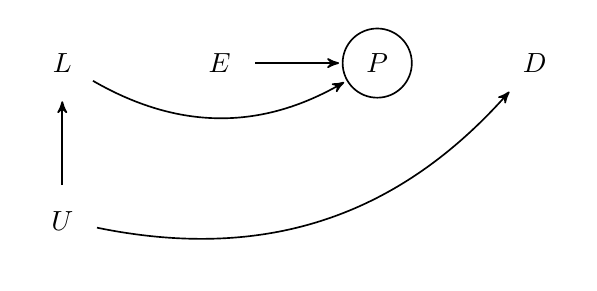
\begin{tikzpicture}[->,>=stealth',shorten >=1pt,auto,node distance=2cm,semithick]
		\node[state,draw = none]         (L)                     {$L$};
		\node[state,draw = none]         (U)    [below of=L]     {$U$};
		\node[state,draw = none]         (E)    [right of=L]     {$E$};
		\node[state,circle]              (P)    [right of=E]     {$P$};
		\node[state,draw = none]         (D)    [right of=P]     {$D$};
		\path (U)   edge  [bend right]   node {} (D)
                    edge                 node {} (L)
              (L)   edge  [bend right]   node {} (P)
              (E)   edge                 node {} (P);
        \end{tikzpicture}
    }
    \caption{}
    \label{fig:f1a}
\end{subfigure}
\begin{subfigure}[b]{0.32\textwidth}
	\centering
	\resizebox{\linewidth}{!}{
		\begin{tikzpicture}[->,>=stealth',shorten >=1pt,auto,node distance=2cm,semithick]
		\node[state,draw = none]         (Us)                    {$U^{*}$};
		\node[state,draw = none]         (E)    [below of=Us]    {$E$};
		\node[state,draw = none]         (U)    [below of=E]     {$U$};
		\node[state,draw = none]         (L)    [right of=E]     {$L$};
		\node[state,circle]              (P)    [right of=L]     {$P$};
		\node[state,draw = none]         (D)    [right of=P]     {$D$};
		\path (Us)  edge                 node {} (E)
		            edge                 node {} (L)
		      (U)   edge  [bend right]   node {} (D)
		            edge                 node {} (L)
		      (L)   edge                 node {} (P);
		\end{tikzpicture}
	}
    \caption{}
	\label{fig:f1b}
\end{subfigure}
\begin{subfigure}[b]{0.32\textwidth}
	\centering
	\resizebox{\linewidth}{!}{
		\begin{tikzpicture}[->,>=latex',shorten >=1pt,auto,node distance=2cm,semithick]
		\node[state,draw = none]         (L)                     {$L$};
		\node[state,draw = none]         (E)    [below of=L]     {$E$};
		\node[state,circle]              (P)    [right of=L]     {$P$};
		\node[]                          (x1)   [right of=P]     {};
		\node[]                          (x2)   [right of=x1]    {};
		\node[state,draw = none]         (D)    [below of=x2]    {$D$};
		
		\path (L)   edge                 node {} (P)
		            edge                 node {} (P)
		      (E)   edge                 node {} (D);
		      
		\draw (L)                    --  node {} ($(E)!0.5!(D)$);
		\end{tikzpicture}
	}
	\caption{}
	\label{fig:f1c}
\end{subfigure}

%\begin{tikzpicture}[->,>=stealth',shorten >=1pt,auto,node distance=2.5cm,semithick]
%
%\node[state,draw = none]         (U*)              {$U^{*}$};
%\node[state,draw = none]         (M) [below of=U*] {$M$};
%\node[state,draw = none]         (E) [right of=M]  {$E$};
%\node[state,circle]              (C) [right of=E]  {$C$};
%\node[state,draw = none]         (O) [right of=C]  {$O$};
%\node[state,draw = none]         (U) [below of=M]  {$U$};

%\path (U*) edge              node {} (E)
%edge              node {} (C)
%(M)  edge [bend right] node {} (C)
%(U)  edge              node {} (M)
%edge [bend right] node {} (O);
%\end{tikzpicture}

 
	\caption{Directed acyclic graph of bias due to self selection or loss to follow up in prospective cohort studies. A spurious association between exposure $E$ and outcome $D$ occurs when (continued) participation $P$ is a common effect of exposure $E$ and participation indicators $L$, and $L$ and the outcome $D$ share an unobserved common cause $U$. \protect\circled{$P$} indicates conditioning on $P$, which opens a collider\supercite{Cole2010-za}, resulting in a spurious association between $D$ to $E$. Panel (a) depicts a situation where $L$ and $E$ are independent as long as there is no conditioning on $P$. This type of bias can be corrected by adjusting for variables $L$ or through multilevel regression and post stratification. (b) When $E$ and $L$ share an unobserved common cause, bias can only be corrected with inverse probability weighting. Panel (c) depicts bias due to effect modification through variables that also determine participation. This bias can emerge in the absence of unobserved variables and can be corrected through adjusted regression and post stratification or by modeling the interaction between $L$ and $E$. (Panels (a) and (b) modified from \citeauthor{Hernan2004-oz}\supercite{Hernan2004-oz}.}
	\label{fig:SelectionBias}
\end{figure}


Figure 1 highlights that bias due to self selection and loss to follow up depends on the covariation of variables included in an analysis with each other and with unobserved causes. Therefore, the presence or absence of bias cannot be determined for an entire cohort study that measures different exposures and outcomes. Instead, it has to be determined for each exposure-outcome-pair. Acquiring information about associations that determine selection bias is non-trivial, because \emph{unobserved} common causes of participation indicators and outcome are central. Common causes can be of environmental\supercite{Johnson2011-wi,Verweij2013-xk} or genetic nature. Genetic correlation coefficients ($r_G$) from twin\supercite{Tambs2012-km} or genome wide association studies \supercite{Bulik-Sullivan2015-er}, which can serve as indicators of common genetic causes, are more widely reported. For instance, single nucleotide polymorphism (SNP) based genetic correlations of $r_{G_{SNP}}=0.01$ and $r_{G_{SNP}}=0.731$ between education and birth-weight or childhood IQ, respectively, were reported\supercite{Bulik-Sullivan2015-xn}. Hence, if one uses a study sample that over-represents well-educated mothers to examine associations between maternal depression and birth weight or childhood IQ, the latter association is more likely biased.

A limitation of the structural approach is that it provides no estimate of bias-magnitude. When population wide data about exposures and outcomes is unavailable, one can estimate bias-magnitude by comparing association estimates obtained with and without controlling for selection bias. Selection bias can be corrected by adjusting for participation indicators (adjusted regression, AR), by stratified analysis and post-stratification  (e.g., multilevel regression and post stratification, MRP\supercite{Gelman2007-hx}), and by weighting individuals according to the inverse participation-probability (inverse probability weighting, IPW\supercite{Seaman2013-rj}). While IPW corrects all types of selection bias displayed in Figure \ref{fig:SelectionBias}, MRP corrects bias due to effect modification and structural bias when the exposure does not cause or share a common cause with participation indicators (as in Figures \ref{fig:f1a} and \ref{fig:f1c}), and AR only corrects bias when the exposure does not cause or share a common cause with participation indicators (c.f. Figure \ref{fig:f1a}). AR and MRP cannot correct selection bias when the exposure causes or shares a common cause with participation indicators (c.f. Figure \ref{fig:f1b}) because conditioning on colliders introduces bias \supercite{Cole2010-za}.

In the remainder of the article we use the association between parental characteristics and preschoolers' ADHD symptoms in the Norwegian Mother and Child Cohort study as an example to demonstrate assessment of bias due to self selection and loss to follow up in a large prospective cohort study. We estimate the joint effects of self selection and loss to follow up by assessing bias in the study population for which outcome data is available, because both biases are present in longitudinal studies.

\section{Methods}

\subsection{Background population and study sample}

\paragraph{Study sample} MoBa is a prospective population-based pregnancy cohort study conducted by the Norwegian Institute of Public Health \supercite{Magnus2006-jj,Magnus2016-ht}. Participating mothers from all over Norway were recruited during routine ultrasound assessment in week 17 or 18 of their pregnancy in the period from 1999 to 2009. 41\% of the invited women consented to participation. MoBa participants received questionnaires in gestational week 17 or 18, week 22 and week 30, at child's age 6 and 18 months, 3, 5, and 8 years and onward (questionnaires available at http://www.fhi.no/moba). The study is still ongoing. The reported analyses also use information from the Medical Birth Registry of Norway (MBRN)\supercite{Irgens2000-ra}, with data on all births in Norway.

The current analysis uses data from the main inclusion period from January 2001 to December 2009, in which 94373 mothers returned the 1st MoBa questionnaire around the 20th pregnancy week. Of these 55763 (59\%) also returned the 6th MoBa questionnaire (at child age 3 years). Table \ref{table:age_edu} shows age and education of the analyzed MoBa sample.

\begin{table}[ht]
	% latex table generated in R 3.4.1 by xtable 1.8-3 package
% Mon Jan 28 15:18:59 2019
\centering
\begin{tabular}{lllrrrrrr}
  \hline
Group & Education & $<$20 & 20-24 & 25-29 & 30-34 & 35-39 & 40-49 & All \\ 
  \hline
MoBa & Elementary & 0.2 & 0.4 & 0.4 & 0.4 & 0.2 & 0.1 & 1.7 \\ 
   & High-school & 0.3 & 6.2 & 9.9 & 8.7 & 4.1 & 0.6 & 29.9 \\ 
   & Bachelor & 0 & 1.8 & 16.7 & 18.0 & 6.2 & 0.8 & 43.7 \\ 
   & Master & 0 & 0.0 & 6.0 & 12.8 & 5.3 & 0.6 & 24.7 \\ 
   & All & 0.6 & 8.4 & 33.1 & 39.9 & 15.9 & 2.1 & 100.0 \\ 
  Population & Elementary & 2 & 5.6 & 5.1 & 3.7 & 1.9 & 0.5 & 18.7 \\ 
   & High-school & 0.3 & 6.8 & 11.9 & 10.3 & 4.6 & 0.8 & 34.7 \\ 
   & Bachelor & 0 & 1.9 & 13.1 & 15.0 & 6.2 & 1.0 & 37.2 \\ 
   & Master & 0 & 0.0 & 1.9 & 4.7 & 2.3 & 0.4 & 9.3 \\ 
   & All & 2.3 & 14.4 & 32.0 & 33.7 & 15.0 & 2.5 & 100.0 \\ 
  Coverage & Elementary & 1.3 & 0.7 & 1.0 & 1.3 & 1.4 & 1.3 & 1.0 \\ 
   & High-school & 12.4 & 10.3 & 9.4 & 9.5 & 10.1 & 9.1 & 9.7 \\ 
   & Bachelor & - & 10.6 & 14.4 & 13.5 & 11.4 & 9.3 & 13.2 \\ 
   & Master & - &  & 35.1 & 30.4 & 25.8 & 19.5 & 29.8 \\ 
   & All & 2.8 & 6.6 & 11.6 & 13.3 & 11.9 & 9.3 & 11.3 \\ 
   \hline
\end{tabular}

	\label{table:age_edu}
\end{table}

\paragraph{Socioeconomic data about the source population}
We obtained aggregated data about age, educational level, and number of children in the household for all women who became mothers in the sampling period of the MoBa from Statistics Norway (SSB). 


\subsection{Statistical analysis}

\paragraph{Investigating unobserved common causes with LD score regression} We used linkage disequilibrium (LD) score regressions \supercite{Bulik-Sullivan2015-er} to calculate genetic correlations between indicators of participation, exposures, and outcome from summary results of genome wide association studies (GWAS). Table \ref{tab:gwas} lists phenotypes for which we obtained GWAS summary data. Genetic correlations also provide information about common causes of maternal characteristics and child phenotypes because mothers and their children share 50\% of their genes.

\paragraph{Outcome, exposures, and control variables} We calculated the outcome variable "ADHD symptom score" by summing the responses (Not, Somewhat or Very often true, coded as 0, 1, 2) to 11 questions about ADHD symptoms that mothers' answered when the child was around 3 years old. Three separate analyses examined the magnitude of selection bias when estimating the effect of (a) birth-related outcomes, (b) maternal and paternal use of legal drugs, and (c) maternal and paternal mental health and use of illegal drugs on preschoolers' ADHD score. Table \ref{table:variables} describes the variables used in the analyses, including a number of control variables as well as transformations applied. 

Mothers\textquotesingle \space mental health was measured as sum scores of the short forms of the symptom check list (SCL)\supercite{Tambs1993-ch} and the lifetime history of depression questionnaire (LTH-5)\supercite{Kendler1993-pf}. Use of illegal drugs (cannabis, ecstasy, amphetamines, cocaine) before or in the pregnancy was assessed with Likert scales (fewer than 0.01\% indicated to having used heroin). Ability scores resulting from an item response theory analysis of these variables \supercite{Rizopoulos2006-bc} were used as predictors in the regression analysis. 

\begin{tabular}{lllll}
		\hline
		Type & Variable & Description & Source & Used in\\ 
		\hline
		\multicolumn{5}{l}{Outcome:} \\
		& child ADHD & SS ADHD symptom ratings & Q6 & IAU\\ 
		\multicolumn{5}{l}{Exposures, birth-related:} \\
		& small f. gest. age & 1 = among 5\% lightest in gest. wk. & MBRN & IAU\\ 
		& preterm & 1 = birthweek $<$ 37 & MBRN & IAU\\ 
		\multicolumn{5}{l}{Exposures, Parental mental health:} \\
		& m. drug use & used any drug 1 = yes, no = 0 & Q1 & IAU\\ 
		& m. drug use score & ability score from IRT model & Q1 & IAU\\ 
		& m. LTH & SS Lifetime History of Depression & Q1 & IAU\\ 
		& m. SCL5 & SS Symptom Check list & Q1 & IAU\\ 
		& p. drug use & used any drug 1 = yes, no = 0 & QF & IAU\\ 
		& p. drug use score & ability score from IRT model & QF & IAU\\ 
		\multicolumn{5}{l}{Exposures, parental use of legal drugs:} \\
		& m. smoking & smoking in pregn.: 1 = yes, 0 = no & Q1 & IAU\\ 
		& m. num. cigarettes & cigarettes per day in pregnancy & Q1 & IAU\\ 
		& m. alc. freq. & in pregnancy, 3 ordered categories & Q1 & IAU\\ 
		& m. eff. units. alc. & effective units of alcohol & Q1 & IAU\\ 
		& p. smoking & smoking, 1 = yes, 0 = no & QF & IAU\\ 
		& p. num. cigarettes & cigarettes per day & QF & IAU\\ 
		& p. alc. freq. & drinking per week & QF & IAU\\ 
		& p. typ. units. alc. & typical number of units alcohol  & QF & IAU\\
		\multicolumn{5}{l}{Adjustment variables:} \\ 
		& child sex & 0 = boys, 1 = girls & MBRN & IA\\ 
		& m. BMI deviat. & log(BMI/mode of BMI) & Q1 & IA \\ 
		& m. ADHD & SS ASRS & Q6 & IA \\ 
		& p. ADHD & SS ASRS & QF & IA \\
		& p. age & 8 ordered categories & QF & IA \\ 
		& p. education & 4 ordered categories & QF & IA \\ 
		\multicolumn{5}{l}{Participation predictors:} \\ 
		& m. education & 4 ordered categories & Q1  & I$_S$A\\ 
		& m. age & 6 ordered categories & Q1  & I$_S$A\\ 
		& Parity & number of children born & MBRN  & I$_S$A\\ 
		\hline
	\end{tabular}

All presented analyses are based on participants for which at least 50 \% of the analysis variables were available. We created 20 multiply imputed data sets with the R package mi \supercite{Su2011-he}. 

\paragraph{Regression model and bias estimation}

In brief, the analysis involves simultaneous estimation of parameters for a regression model with inverse probability weighting (IPW) and an adjusted regression (AR) model, where the AR model adjusts for the participation indicators used in the selection model. To account for covariation of regression weights, weights for the AR model are defined as  weights for the IPW model plus a difference term. Because ADHD sum scores are constraint to be between 0 and 22, we used a beta binomial regression model and report results as average marginal effects (AMEs), because these are more intuitive than regression weights on a multiplicative scale. 

Smoothed inverse probability weights were calculated from results of a hierarchical binomial regression\supercite{Stan_Development_Team_2016-te} of MoBa participation on the indicators parity, mothers' age, and education (c.f. \ref{fig:IPW}). All analyses used the same set of control variables (c.f. \ref{table:variables}) except that only the AR analysis adjusted for participation indicators.

We calculate bias by dividing the difference between the AME estimates of the IPW and AR models with either the standard deviation or the mean of the IPW estimate. Both approaches have been used previously\supercite{Stuart2010-cj,Nilsen2009-ci}, the former appeals to the intuition that bias is problematic if the true parameters high certainty, whereas the latter appeals to the intuition that bias is problematic if it has a large deviation from the true parameter. To test for bias, we check how much of the posterior distribution of the bias lies within a region of practical equivalence (ROPE), i.e. in a range of bias that is for practical purposes equivalent with zero \supercite{Kruschke2010-zi, Mascha2011-um}. This also allows quantifying the risk for substantial bias as the ratio of the posterior probabilities of the bias estimate being inside and outside the ROPE. Similar to earlier research, which defined deviations of larger than 30 or 40\% of the standard deviation or mean of comparison standard as problematic\supercite{Stuart2010-cj,Nohr2006-uf}, we biases of less than 0.5 as practically equivalent with zero.

Regression analyses were performed with custom models implemented in Stan \supercite{Stan_Development_Team2017-lp} and fit with RStan\supercite{Stan_Development_Team2017-lp}.

\section{Results}

Statistics Norway recorded 510\,561 women who became mothers in the period from 2001 to 2009. In the same period, 94\,373 mothers returned the first MoBa questionnaire (Q1). Of these, 55\,763 also returned the sixth questionnaire,  which was sent out when  children were 3 years old. 54\,557 returned questionnaires with fewer than 50\% missing data among the variables of interest. The participants included in the reported analysis constitute around 14\% of the source population.

\subsection*{Socio-demographic composition of study sample and population}
 Mothers with elementary school education or less constitute around 18.7\% of the population but only 1.7\% of the MoBa sample (see Table \ref{table:age_edu}). 16.6\% of mothers in the population are younger than 25, compared to around 9.1\% in the MoBa samples. Accordingly, the participation rates vary substantially between population subgroups: 23.8\% of mothers with a master's degree participated in MoBa, but only around 0.8\% of mothers with elementary school education. For parity, the difference between MoBa and population is less pronounced. The percentages of women in the population (MoBa) who had previously 0, 1, 2, or 3 or more pregnancies are 41.8 (50.9), 36.3 (32.5), 16.1 (13.9), 2.8 (5.8), respectively. Hence, MoBa over-represents mothers of firstborn children and under-represents those with more than two children.

\subsection*{Inverse probability weights}
The hierarchical binomial model captured participation well, as indicated by a correlation of $r=0.99$ between modeled and observed participation rates (see Figure \ref{fig:IPW}). The mothers's education was the key variable to predict participation. Smoothed weights ranged between on average 0.31 and 21.36. The largest weights were for mothers with only elementary school education, and the smallest for mothers with a master's degree. We chose not to trim weights, because this would result in improper weighting of the study sample.

\subsection*{Unobserved genetic common causes}
LD score regression results indicate unobserved common genetic causes of participation indicators and outcome or exposures, respectively (see Figure \ref{fig:rg}). For example, genes associated with "age at first birth" or "years of education" are also (negatively) associated with ADHD, maternal mental health, or smoking. The overall SNP based heritability is generally not high, and often below 10\%.

\begin{figure}
	\begin{center}
		% Created by tikzDevice version 0.12 on 2019-01-25 19:24:20
% !TEX encoding = UTF-8 Unicode
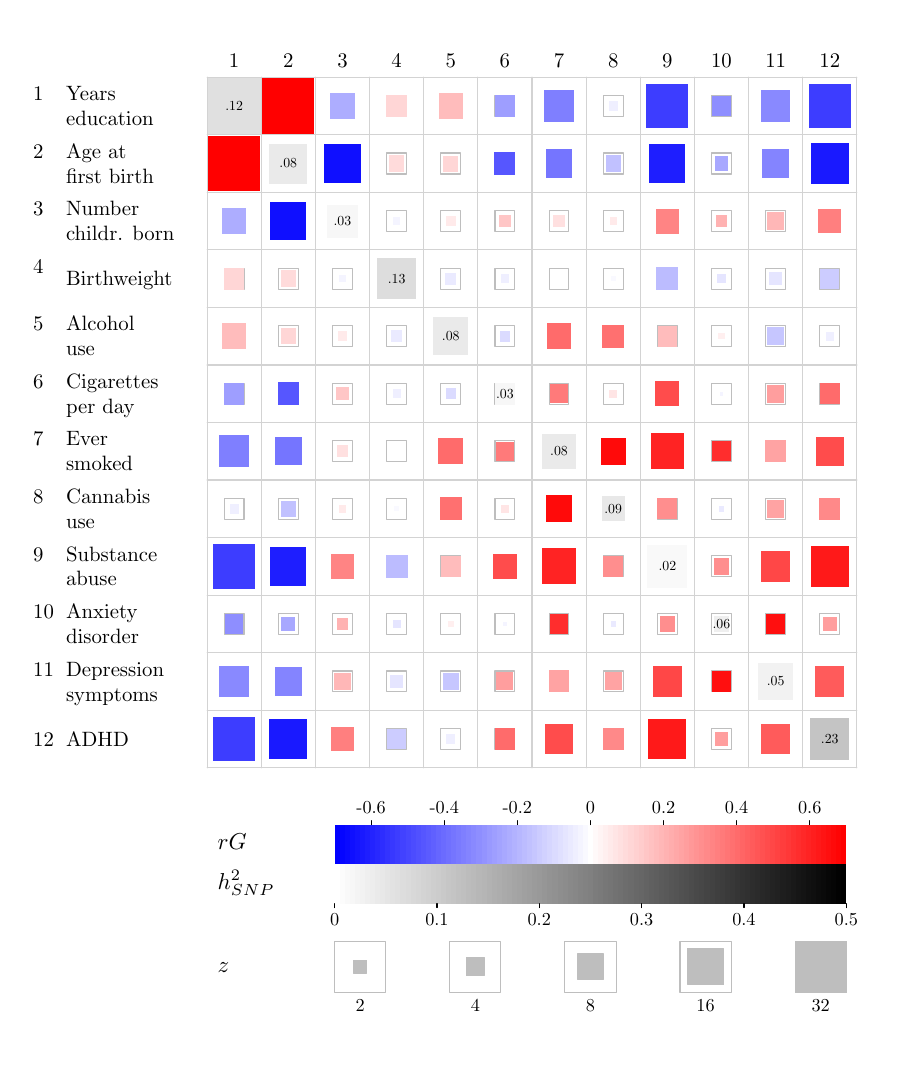
\begin{tikzpicture}[x=1pt,y=1pt]
\definecolor{fillColor}{RGB}{255,255,255}
\path[use as bounding box,fill=fillColor,fill opacity=0.00] (0,0) rectangle (312.98,369.89);
\begin{scope}
\path[clip] ( 55.44, 92.47) rectangle (309.02,361.97);
\definecolor{drawColor}{RGB}{190,190,190}
\definecolor{fillColor}{RGB}{255,255,255}

\path[draw=drawColor,line width= 0.4pt,line join=round,line cap=round,fill=fillColor] (110.19,317.01) rectangle (117.31,324.58);
\definecolor{fillColor}{RGB}{15,15,255}

\path[fill=fillColor] (107.18,313.82) rectangle (120.31,327.77);
\definecolor{fillColor}{RGB}{255,255,255}

\path[draw=drawColor,line width= 0.4pt,line join=round,line cap=round,fill=fillColor] ( 90.62,296.21) rectangle ( 97.74,303.78);
\definecolor{fillColor}{RGB}{15,15,255}

\path[fill=fillColor] ( 87.62,293.02) rectangle (100.75,306.98);
\definecolor{fillColor}{RGB}{255,255,255}

\path[draw=drawColor,line width= 0.4pt,line join=round,line cap=round,fill=fillColor] (286.28,317.01) rectangle (293.41,324.58);
\definecolor{fillColor}{RGB}{25,25,255}

\path[fill=fillColor] (283.01,313.53) rectangle (296.68,328.06);
\definecolor{fillColor}{RGB}{255,255,255}

\path[draw=drawColor,line width= 0.4pt,line join=round,line cap=round,fill=fillColor] ( 90.62,109.06) rectangle ( 97.74,116.64);
\definecolor{fillColor}{RGB}{25,25,255}

\path[fill=fillColor] ( 87.35,105.59) rectangle (101.02,120.11);
\definecolor{fillColor}{RGB}{255,255,255}

\path[draw=drawColor,line width= 0.4pt,line join=round,line cap=round,fill=fillColor] (227.58,317.01) rectangle (234.71,324.58);
\definecolor{fillColor}{RGB}{30,30,255}

\path[fill=fillColor] (224.62,313.86) rectangle (237.67,327.73);
\definecolor{fillColor}{RGB}{255,255,255}

\path[draw=drawColor,line width= 0.4pt,line join=round,line cap=round,fill=fillColor] ( 90.62,171.45) rectangle ( 97.74,179.02);
\definecolor{fillColor}{RGB}{30,30,255}

\path[fill=fillColor] ( 87.66,168.30) rectangle (100.71,182.17);
\definecolor{fillColor}{RGB}{255,255,255}

\path[draw=drawColor,line width= 0.4pt,line join=round,line cap=round,fill=fillColor] (286.28,337.80) rectangle (293.41,345.37);
\definecolor{fillColor}{RGB}{61,61,255}

\path[fill=fillColor] (282.21,333.48) rectangle (297.48,349.70);
\definecolor{fillColor}{RGB}{255,255,255}

\path[draw=drawColor,line width= 0.4pt,line join=round,line cap=round,fill=fillColor] (227.58,337.80) rectangle (234.71,345.37);
\definecolor{fillColor}{RGB}{61,61,255}

\path[fill=fillColor] (223.58,333.55) rectangle (238.71,349.62);
\definecolor{fillColor}{RGB}{255,255,255}

\path[draw=drawColor,line width= 0.4pt,line join=round,line cap=round,fill=fillColor] ( 71.05,109.06) rectangle ( 78.18,116.64);
\definecolor{fillColor}{RGB}{61,61,255}

\path[fill=fillColor] ( 66.98,104.74) rectangle ( 82.25,120.96);
\definecolor{fillColor}{RGB}{255,255,255}

\path[draw=drawColor,line width= 0.4pt,line join=round,line cap=round,fill=fillColor] ( 71.05,171.45) rectangle ( 78.18,179.02);
\definecolor{fillColor}{RGB}{61,61,255}

\path[fill=fillColor] ( 67.05,167.20) rectangle ( 82.18,183.27);
\definecolor{fillColor}{RGB}{255,255,255}

\path[draw=drawColor,line width= 0.4pt,line join=round,line cap=round,fill=fillColor] (168.88,317.01) rectangle (176.01,324.58);
\definecolor{fillColor}{RGB}{86,86,255}

\path[fill=fillColor] (168.63,316.73) rectangle (176.27,324.85);
\definecolor{fillColor}{RGB}{255,255,255}

\path[draw=drawColor,line width= 0.4pt,line join=round,line cap=round,fill=fillColor] ( 90.62,233.83) rectangle ( 97.74,241.40);
\definecolor{fillColor}{RGB}{86,86,255}

\path[fill=fillColor] ( 90.36,233.55) rectangle ( 98.00,241.68);
\definecolor{fillColor}{RGB}{255,255,255}

\path[draw=drawColor,line width= 0.4pt,line join=round,line cap=round,fill=fillColor] (188.45,317.01) rectangle (195.58,324.58);
\definecolor{fillColor}{RGB}{117,117,255}

\path[fill=fillColor] (187.19,315.66) rectangle (196.84,325.92);
\definecolor{fillColor}{RGB}{255,255,255}

\path[draw=drawColor,line width= 0.4pt,line join=round,line cap=round,fill=fillColor] ( 90.62,213.04) rectangle ( 97.74,220.61);
\definecolor{fillColor}{RGB}{117,117,255}

\path[fill=fillColor] ( 89.36,211.69) rectangle ( 99.01,221.95);
\definecolor{fillColor}{RGB}{255,255,255}

\path[draw=drawColor,line width= 0.4pt,line join=round,line cap=round,fill=fillColor] ( 71.05,213.04) rectangle ( 78.18,220.61);
\definecolor{fillColor}{RGB}{127,127,255}

\path[fill=fillColor] ( 69.24,211.11) rectangle ( 79.99,222.54);
\definecolor{fillColor}{RGB}{255,255,255}

\path[draw=drawColor,line width= 0.4pt,line join=round,line cap=round,fill=fillColor] (188.45,337.80) rectangle (195.58,345.37);
\definecolor{fillColor}{RGB}{127,127,255}

\path[fill=fillColor] (186.64,335.87) rectangle (197.39,347.30);
\definecolor{fillColor}{RGB}{255,255,255}

\path[draw=drawColor,line width= 0.4pt,line join=round,line cap=round,fill=fillColor] (266.72,317.01) rectangle (273.84,324.58);
\definecolor{fillColor}{RGB}{132,132,255}

\path[fill=fillColor] (265.42,315.63) rectangle (275.14,325.96);
\definecolor{fillColor}{RGB}{255,255,255}

\path[draw=drawColor,line width= 0.4pt,line join=round,line cap=round,fill=fillColor] ( 90.62,129.86) rectangle ( 97.74,137.43);
\definecolor{fillColor}{RGB}{132,132,255}

\path[fill=fillColor] ( 89.32,128.48) rectangle ( 99.04,138.81);
\definecolor{fillColor}{RGB}{255,255,255}

\path[draw=drawColor,line width= 0.4pt,line join=round,line cap=round,fill=fillColor] (266.72,337.80) rectangle (273.84,345.37);
\definecolor{fillColor}{RGB}{137,137,255}

\path[fill=fillColor] (264.94,335.92) rectangle (275.61,347.26);
\definecolor{fillColor}{RGB}{255,255,255}

\path[draw=drawColor,line width= 0.4pt,line join=round,line cap=round,fill=fillColor] ( 71.05,129.86) rectangle ( 78.18,137.43);
\definecolor{fillColor}{RGB}{137,137,255}

\path[fill=fillColor] ( 69.28,127.98) rectangle ( 79.95,139.31);
\definecolor{fillColor}{RGB}{255,255,255}

\path[draw=drawColor,line width= 0.4pt,line join=round,line cap=round,fill=fillColor] (247.15,337.80) rectangle (254.27,345.37);
\definecolor{fillColor}{RGB}{142,142,255}

\path[fill=fillColor] (247.37,338.04) rectangle (254.05,345.13);
\definecolor{fillColor}{RGB}{255,255,255}

\path[draw=drawColor,line width= 0.4pt,line join=round,line cap=round,fill=fillColor] ( 71.05,150.65) rectangle ( 78.18,158.22);
\definecolor{fillColor}{RGB}{142,142,255}

\path[fill=fillColor] ( 71.28,150.89) rectangle ( 77.95,157.99);
\definecolor{fillColor}{RGB}{255,255,255}

\path[draw=drawColor,line width= 0.4pt,line join=round,line cap=round,fill=fillColor] (168.88,337.80) rectangle (176.01,345.37);
\definecolor{fillColor}{RGB}{158,158,255}

\path[fill=fillColor] (168.76,337.67) rectangle (176.13,345.51);
\definecolor{fillColor}{RGB}{255,255,255}

\path[draw=drawColor,line width= 0.4pt,line join=round,line cap=round,fill=fillColor] ( 71.05,233.83) rectangle ( 78.18,241.40);
\definecolor{fillColor}{RGB}{158,158,255}

\path[fill=fillColor] ( 70.93,233.70) rectangle ( 78.30,241.53);
\definecolor{fillColor}{RGB}{255,255,255}

\path[draw=drawColor,line width= 0.4pt,line join=round,line cap=round,fill=fillColor] (247.15,317.01) rectangle (254.27,324.58);
\definecolor{fillColor}{RGB}{168,168,255}

\path[fill=fillColor] (248.22,318.15) rectangle (253.20,323.44);
\definecolor{fillColor}{RGB}{255,255,255}

\path[draw=drawColor,line width= 0.4pt,line join=round,line cap=round,fill=fillColor] ( 90.62,150.65) rectangle ( 97.74,158.22);
\definecolor{fillColor}{RGB}{168,168,255}

\path[fill=fillColor] ( 91.69,151.79) rectangle ( 96.67,157.09);
\definecolor{fillColor}{RGB}{255,255,255}

\path[draw=drawColor,line width= 0.4pt,line join=round,line cap=round,fill=fillColor] ( 71.05,296.21) rectangle ( 78.18,303.78);
\definecolor{fillColor}{RGB}{173,173,255}

\path[fill=fillColor] ( 70.24,295.35) rectangle ( 78.99,304.65);
\definecolor{fillColor}{RGB}{255,255,255}

\path[draw=drawColor,line width= 0.4pt,line join=round,line cap=round,fill=fillColor] (110.19,337.80) rectangle (117.31,345.37);
\definecolor{fillColor}{RGB}{173,173,255}

\path[fill=fillColor] (109.37,336.94) rectangle (118.12,346.24);
\definecolor{fillColor}{RGB}{255,255,255}

\path[draw=drawColor,line width= 0.4pt,line join=round,line cap=round,fill=fillColor] (227.58,275.42) rectangle (234.71,282.99);
\definecolor{fillColor}{RGB}{188,188,255}

\path[fill=fillColor] (227.21,275.03) rectangle (235.08,283.38);
\definecolor{fillColor}{RGB}{255,255,255}

\path[draw=drawColor,line width= 0.4pt,line join=round,line cap=round,fill=fillColor] (129.75,171.45) rectangle (136.88,179.02);
\definecolor{fillColor}{RGB}{188,188,255}

\path[fill=fillColor] (129.38,171.05) rectangle (137.25,179.41);
\definecolor{fillColor}{RGB}{255,255,255}

\path[draw=drawColor,line width= 0.4pt,line join=round,line cap=round,fill=fillColor] (208.02,317.01) rectangle (215.14,324.58);
\definecolor{fillColor}{RGB}{193,193,255}

\path[fill=fillColor] (208.85,317.89) rectangle (214.31,323.70);
\definecolor{fillColor}{RGB}{255,255,255}

\path[draw=drawColor,line width= 0.4pt,line join=round,line cap=round,fill=fillColor] ( 90.62,192.24) rectangle ( 97.74,199.81);
\definecolor{fillColor}{RGB}{193,193,255}

\path[fill=fillColor] ( 91.45,193.12) rectangle ( 96.91,198.93);
\definecolor{fillColor}{RGB}{255,255,255}

\path[draw=drawColor,line width= 0.4pt,line join=round,line cap=round,fill=fillColor] (149.32,129.86) rectangle (156.44,137.43);
\definecolor{fillColor}{RGB}{198,198,255}

\path[fill=fillColor] (149.92,130.50) rectangle (155.84,136.79);
\definecolor{fillColor}{RGB}{255,255,255}

\path[draw=drawColor,line width= 0.4pt,line join=round,line cap=round,fill=fillColor] (266.72,254.62) rectangle (273.84,262.20);
\definecolor{fillColor}{RGB}{198,198,255}

\path[fill=fillColor] (267.32,255.26) rectangle (273.24,261.56);
\definecolor{fillColor}{RGB}{255,255,255}

\path[draw=drawColor,line width= 0.4pt,line join=round,line cap=round,fill=fillColor] (286.28,275.42) rectangle (293.41,282.99);
\definecolor{fillColor}{RGB}{204,204,255}

\path[fill=fillColor] (286.48,275.62) rectangle (293.22,282.79);
\definecolor{fillColor}{RGB}{255,255,255}

\path[draw=drawColor,line width= 0.4pt,line join=round,line cap=round,fill=fillColor] (129.75,109.06) rectangle (136.88,116.64);
\definecolor{fillColor}{RGB}{204,204,255}

\path[fill=fillColor] (129.94,109.27) rectangle (136.68,116.43);
\definecolor{fillColor}{RGB}{255,255,255}

\path[draw=drawColor,line width= 0.4pt,line join=round,line cap=round,fill=fillColor] (149.32,233.83) rectangle (156.44,241.40);
\definecolor{fillColor}{RGB}{219,219,255}

\path[fill=fillColor] (151.04,235.66) rectangle (154.72,239.58);
\definecolor{fillColor}{RGB}{255,255,255}

\path[draw=drawColor,line width= 0.4pt,line join=round,line cap=round,fill=fillColor] (168.88,254.62) rectangle (176.01,262.20);
\definecolor{fillColor}{RGB}{219,219,255}

\path[fill=fillColor] (170.60,256.45) rectangle (174.29,260.37);
\definecolor{fillColor}{RGB}{255,255,255}

\path[draw=drawColor,line width= 0.4pt,line join=round,line cap=round,fill=fillColor] (129.75,150.65) rectangle (136.88,158.22);
\definecolor{fillColor}{RGB}{229,229,255}

\path[fill=fillColor] (131.87,152.90) rectangle (134.76,155.98);
\definecolor{fillColor}{RGB}{255,255,255}

\path[draw=drawColor,line width= 0.4pt,line join=round,line cap=round,fill=fillColor] (129.75,129.86) rectangle (136.88,137.43);
\definecolor{fillColor}{RGB}{229,229,255}

\path[fill=fillColor] (131.00,131.18) rectangle (135.63,136.11);
\definecolor{fillColor}{RGB}{255,255,255}

\path[draw=drawColor,line width= 0.4pt,line join=round,line cap=round,fill=fillColor] (247.15,275.42) rectangle (254.27,282.99);
\definecolor{fillColor}{RGB}{229,229,255}

\path[fill=fillColor] (249.26,277.67) rectangle (252.16,280.74);
\definecolor{fillColor}{RGB}{255,255,255}

\path[draw=drawColor,line width= 0.4pt,line join=round,line cap=round,fill=fillColor] (266.72,275.42) rectangle (273.84,282.99);
\definecolor{fillColor}{RGB}{229,229,255}

\path[fill=fillColor] (267.96,276.74) rectangle (272.60,281.67);
\definecolor{fillColor}{RGB}{255,255,255}

\path[draw=drawColor,line width= 0.4pt,line join=round,line cap=round,fill=fillColor] (149.32,275.42) rectangle (156.44,282.99);
\definecolor{fillColor}{RGB}{234,234,255}

\path[fill=fillColor] (150.83,277.02) rectangle (154.93,281.39);
\definecolor{fillColor}{RGB}{255,255,255}

\path[draw=drawColor,line width= 0.4pt,line join=round,line cap=round,fill=fillColor] (208.02,150.65) rectangle (215.14,158.22);
\definecolor{fillColor}{RGB}{234,234,255}

\path[fill=fillColor] (210.63,153.43) rectangle (212.53,155.45);
\definecolor{fillColor}{RGB}{255,255,255}

\path[draw=drawColor,line width= 0.4pt,line join=round,line cap=round,fill=fillColor] (129.75,254.62) rectangle (136.88,262.20);
\definecolor{fillColor}{RGB}{234,234,255}

\path[fill=fillColor] (131.26,256.23) rectangle (135.37,260.59);
\definecolor{fillColor}{RGB}{255,255,255}

\path[draw=drawColor,line width= 0.4pt,line join=round,line cap=round,fill=fillColor] (247.15,192.24) rectangle (254.27,199.81);
\definecolor{fillColor}{RGB}{234,234,255}

\path[fill=fillColor] (249.76,195.02) rectangle (251.66,197.04);
\definecolor{fillColor}{RGB}{255,255,255}

\path[draw=drawColor,line width= 0.4pt,line join=round,line cap=round,fill=fillColor] (149.32,109.06) rectangle (156.44,116.64);
\definecolor{fillColor}{RGB}{239,239,255}

\path[fill=fillColor] (151.33,111.20) rectangle (154.43,114.50);
\definecolor{fillColor}{RGB}{255,255,255}

\path[draw=drawColor,line width= 0.4pt,line join=round,line cap=round,fill=fillColor] (208.02,337.80) rectangle (215.14,345.37);
\definecolor{fillColor}{RGB}{239,239,255}

\path[fill=fillColor] (209.90,339.80) rectangle (213.26,343.37);
\definecolor{fillColor}{RGB}{255,255,255}

\path[draw=drawColor,line width= 0.4pt,line join=round,line cap=round,fill=fillColor] (168.88,275.42) rectangle (176.01,282.99);
\definecolor{fillColor}{RGB}{239,239,255}

\path[fill=fillColor] (170.96,277.62) rectangle (173.93,280.78);
\definecolor{fillColor}{RGB}{255,255,255}

\path[draw=drawColor,line width= 0.4pt,line join=round,line cap=round,fill=fillColor] (286.28,254.62) rectangle (293.41,262.20);
\definecolor{fillColor}{RGB}{239,239,255}

\path[fill=fillColor] (288.30,256.76) rectangle (291.39,260.06);
\definecolor{fillColor}{RGB}{255,255,255}

\path[draw=drawColor,line width= 0.4pt,line join=round,line cap=round,fill=fillColor] ( 71.05,192.24) rectangle ( 78.18,199.81);
\definecolor{fillColor}{RGB}{239,239,255}

\path[fill=fillColor] ( 72.93,194.24) rectangle ( 76.30,197.81);
\definecolor{fillColor}{RGB}{255,255,255}

\path[draw=drawColor,line width= 0.4pt,line join=round,line cap=round,fill=fillColor] (129.75,233.83) rectangle (136.88,241.40);
\definecolor{fillColor}{RGB}{239,239,255}

\path[fill=fillColor] (131.83,236.04) rectangle (134.80,239.20);
\definecolor{fillColor}{RGB}{255,255,255}

\path[draw=drawColor,line width= 0.4pt,line join=round,line cap=round,fill=fillColor] (129.75,296.21) rectangle (136.88,303.78);
\definecolor{fillColor}{RGB}{244,244,255}

\path[fill=fillColor] (132.01,298.61) rectangle (134.62,301.38);
\definecolor{fillColor}{RGB}{255,255,255}

\path[draw=drawColor,line width= 0.4pt,line join=round,line cap=round,fill=fillColor] (168.88,150.65) rectangle (176.01,158.22);
\definecolor{fillColor}{RGB}{244,244,255}

\path[fill=fillColor] (171.75,153.69) rectangle (173.15,155.18);
\definecolor{fillColor}{RGB}{255,255,255}

\path[draw=drawColor,line width= 0.4pt,line join=round,line cap=round,fill=fillColor] (110.19,275.42) rectangle (117.31,282.99);
\definecolor{fillColor}{RGB}{244,244,255}

\path[fill=fillColor] (112.44,277.82) rectangle (115.05,280.59);
\definecolor{fillColor}{RGB}{255,255,255}

\path[draw=drawColor,line width= 0.4pt,line join=round,line cap=round,fill=fillColor] (247.15,233.83) rectangle (254.27,241.40);
\definecolor{fillColor}{RGB}{244,244,255}

\path[fill=fillColor] (250.01,236.87) rectangle (251.41,238.36);
\definecolor{fillColor}{RGB}{255,255,255}

\path[draw=drawColor,line width= 0.4pt,line join=round,line cap=round,fill=fillColor] (208.02,275.42) rectangle (215.14,282.99);
\definecolor{fillColor}{RGB}{249,249,255}

\path[fill=fillColor] (210.68,278.25) rectangle (212.48,280.16);
\definecolor{fillColor}{RGB}{255,255,255}

\path[draw=drawColor,line width= 0.4pt,line join=round,line cap=round,fill=fillColor] (129.75,192.24) rectangle (136.88,199.81);
\definecolor{fillColor}{RGB}{249,249,255}

\path[fill=fillColor] (132.42,195.07) rectangle (134.21,196.98);
\definecolor{fillColor}{RGB}{255,255,255}

\path[draw=drawColor,line width= 0.4pt,line join=round,line cap=round,fill=fillColor] (129.75,213.04) rectangle (136.88,220.61);

\path[fill=fillColor] (132.63,216.09) rectangle (134.00,217.55);

\path[draw=drawColor,line width= 0.4pt,line join=round,line cap=round,fill=fillColor] (188.45,275.42) rectangle (195.58,282.99);

\path[fill=fillColor] (191.33,278.47) rectangle (192.70,279.94);

\path[draw=drawColor,line width= 0.4pt,line join=round,line cap=round,fill=fillColor] (227.58,171.45) rectangle (234.71,179.02);
\definecolor{fillColor}{RGB}{249,249,249}

\path[fill=fillColor] (223.94,167.58) rectangle (238.35,182.89);
\definecolor{drawColor}{RGB}{0,0,0}

\node[text=drawColor,anchor=base,inner sep=0pt, outer sep=0pt, scale=  0.50] at (231.15,173.65) {.02};
\definecolor{drawColor}{RGB}{190,190,190}
\definecolor{fillColor}{RGB}{255,255,255}

\path[draw=drawColor,line width= 0.4pt,line join=round,line cap=round,fill=fillColor] (168.88,233.83) rectangle (176.01,241.40);
\definecolor{fillColor}{gray}{0.97}

\path[fill=fillColor] (168.75,233.68) rectangle (176.15,241.55);
\definecolor{drawColor}{RGB}{0,0,0}

\node[text=drawColor,anchor=base,inner sep=0pt, outer sep=0pt, scale=  0.50] at (172.45,236.03) {.03};
\definecolor{drawColor}{RGB}{190,190,190}
\definecolor{fillColor}{RGB}{255,255,255}

\path[draw=drawColor,line width= 0.4pt,line join=round,line cap=round,fill=fillColor] (110.19,296.21) rectangle (117.31,303.78);
\definecolor{fillColor}{gray}{0.97}

\path[fill=fillColor] (108.13,294.03) rectangle (119.36,305.96);
\definecolor{drawColor}{RGB}{0,0,0}

\node[text=drawColor,anchor=base,inner sep=0pt, outer sep=0pt, scale=  0.50] at (113.75,298.41) {.03};
\definecolor{drawColor}{RGB}{190,190,190}
\definecolor{fillColor}{RGB}{255,255,255}

\path[draw=drawColor,line width= 0.4pt,line join=round,line cap=round,fill=fillColor] (149.32,150.65) rectangle (156.44,158.22);
\definecolor{fillColor}{RGB}{255,239,239}

\path[fill=fillColor] (151.78,153.27) rectangle (153.98,155.61);
\definecolor{fillColor}{RGB}{255,255,255}

\path[draw=drawColor,line width= 0.4pt,line join=round,line cap=round,fill=fillColor] (247.15,254.62) rectangle (254.27,262.20);
\definecolor{fillColor}{RGB}{255,239,239}

\path[fill=fillColor] (249.61,257.24) rectangle (251.82,259.58);
\definecolor{fillColor}{RGB}{255,255,255}

\path[draw=drawColor,line width= 0.4pt,line join=round,line cap=round,fill=fillColor] (266.72,129.86) rectangle (273.84,137.43);
\definecolor{fillColor}{gray}{0.95}

\path[fill=fillColor] (263.92,126.88) rectangle (276.64,140.40);
\definecolor{drawColor}{RGB}{0,0,0}

\node[text=drawColor,anchor=base,inner sep=0pt, outer sep=0pt, scale=  0.50] at (270.28,132.06) {.05};
\definecolor{drawColor}{RGB}{190,190,190}
\definecolor{fillColor}{RGB}{255,255,255}

\path[draw=drawColor,line width= 0.4pt,line join=round,line cap=round,fill=fillColor] (208.02,296.21) rectangle (215.14,303.78);
\definecolor{fillColor}{RGB}{255,234,234}

\path[fill=fillColor] (210.29,298.63) rectangle (212.87,301.37);
\definecolor{fillColor}{RGB}{255,255,255}

\path[draw=drawColor,line width= 0.4pt,line join=round,line cap=round,fill=fillColor] (110.19,192.24) rectangle (117.31,199.81);
\definecolor{fillColor}{RGB}{255,234,234}

\path[fill=fillColor] (112.46,194.66) rectangle (115.04,197.40);
\definecolor{fillColor}{RGB}{255,255,255}

\path[draw=drawColor,line width= 0.4pt,line join=round,line cap=round,fill=fillColor] (149.32,296.21) rectangle (156.44,303.78);
\definecolor{fillColor}{RGB}{255,234,234}

\path[fill=fillColor] (151.10,298.11) rectangle (154.66,301.89);
\definecolor{fillColor}{RGB}{255,255,255}

\path[draw=drawColor,line width= 0.4pt,line join=round,line cap=round,fill=fillColor] (110.19,254.62) rectangle (117.31,262.20);
\definecolor{fillColor}{RGB}{255,234,234}

\path[fill=fillColor] (111.97,256.52) rectangle (115.53,260.30);
\definecolor{fillColor}{RGB}{255,255,255}

\path[draw=drawColor,line width= 0.4pt,line join=round,line cap=round,fill=fillColor] (247.15,150.65) rectangle (254.27,158.22);
\definecolor{fillColor}{RGB}{239,239,239}

\path[fill=fillColor] (247.88,151.43) rectangle (253.54,157.45);
\definecolor{drawColor}{RGB}{0,0,0}

\node[text=drawColor,anchor=base,inner sep=0pt, outer sep=0pt, scale=  0.50] at (250.71,152.85) {.06};
\definecolor{drawColor}{RGB}{190,190,190}
\definecolor{fillColor}{RGB}{255,255,255}

\path[draw=drawColor,line width= 0.4pt,line join=round,line cap=round,fill=fillColor] (208.02,233.83) rectangle (215.14,241.40);
\definecolor{fillColor}{RGB}{255,229,229}

\path[fill=fillColor] (210.23,236.18) rectangle (212.93,239.05);
\definecolor{fillColor}{RGB}{255,255,255}

\path[draw=drawColor,line width= 0.4pt,line join=round,line cap=round,fill=fillColor] (168.88,192.24) rectangle (176.01,199.81);
\definecolor{fillColor}{RGB}{255,229,229}

\path[fill=fillColor] (171.10,194.60) rectangle (173.79,197.46);
\definecolor{fillColor}{RGB}{255,255,255}

\path[draw=drawColor,line width= 0.4pt,line join=round,line cap=round,fill=fillColor] (188.45,213.04) rectangle (195.58,220.61);
\definecolor{fillColor}{RGB}{234,234,234}

\path[fill=fillColor] (186.00,210.43) rectangle (198.03,223.22);
\definecolor{drawColor}{RGB}{0,0,0}

\node[text=drawColor,anchor=base,inner sep=0pt, outer sep=0pt, scale=  0.50] at (192.01,215.23) {.08};
\definecolor{drawColor}{RGB}{190,190,190}
\definecolor{fillColor}{RGB}{255,255,255}

\path[draw=drawColor,line width= 0.4pt,line join=round,line cap=round,fill=fillColor] (188.45,296.21) rectangle (195.58,303.78);
\definecolor{fillColor}{RGB}{255,224,224}

\path[fill=fillColor] (190.00,297.86) rectangle (194.03,302.14);
\definecolor{fillColor}{RGB}{255,255,255}

\path[draw=drawColor,line width= 0.4pt,line join=round,line cap=round,fill=fillColor] (110.19,213.04) rectangle (117.31,220.61);
\definecolor{fillColor}{RGB}{255,224,224}

\path[fill=fillColor] (111.73,214.68) rectangle (115.76,218.96);
\definecolor{fillColor}{RGB}{255,255,255}

\path[draw=drawColor,line width= 0.4pt,line join=round,line cap=round,fill=fillColor] ( 90.62,317.01) rectangle ( 97.74,324.58);
\definecolor{fillColor}{RGB}{234,234,234}

\path[fill=fillColor] ( 87.38,313.57) rectangle (100.98,328.02);
\definecolor{drawColor}{RGB}{0,0,0}

\node[text=drawColor,anchor=base,inner sep=0pt, outer sep=0pt, scale=  0.50] at ( 94.18,319.21) {.08};
\definecolor{drawColor}{RGB}{190,190,190}
\definecolor{fillColor}{RGB}{255,255,255}

\path[draw=drawColor,line width= 0.4pt,line join=round,line cap=round,fill=fillColor] (149.32,254.62) rectangle (156.44,262.20);
\definecolor{fillColor}{RGB}{234,234,234}

\path[fill=fillColor] (146.47,251.59) rectangle (159.29,265.23);
\definecolor{drawColor}{RGB}{0,0,0}

\node[text=drawColor,anchor=base,inner sep=0pt, outer sep=0pt, scale=  0.50] at (152.88,256.82) {.08};
\definecolor{drawColor}{RGB}{190,190,190}
\definecolor{fillColor}{RGB}{255,255,255}

\path[draw=drawColor,line width= 0.4pt,line join=round,line cap=round,fill=fillColor] (208.02,192.24) rectangle (215.14,199.81);
\definecolor{fillColor}{gray}{0.91}

\path[fill=fillColor] (207.39,191.57) rectangle (215.77,200.48);
\definecolor{drawColor}{RGB}{0,0,0}

\node[text=drawColor,anchor=base,inner sep=0pt, outer sep=0pt, scale=  0.50] at (211.58,194.44) {.09};
\definecolor{drawColor}{RGB}{190,190,190}
\definecolor{fillColor}{RGB}{255,255,255}

\path[draw=drawColor,line width= 0.4pt,line join=round,line cap=round,fill=fillColor] (129.75,317.01) rectangle (136.88,324.58);
\definecolor{fillColor}{RGB}{255,219,219}

\path[fill=fillColor] (130.50,317.80) rectangle (136.13,323.79);
\definecolor{fillColor}{RGB}{255,255,255}

\path[draw=drawColor,line width= 0.4pt,line join=round,line cap=round,fill=fillColor] ( 90.62,275.42) rectangle ( 97.74,282.99);
\definecolor{fillColor}{RGB}{255,219,219}

\path[fill=fillColor] ( 91.36,276.21) rectangle ( 97.00,282.20);
\definecolor{fillColor}{RGB}{255,255,255}

\path[draw=drawColor,line width= 0.4pt,line join=round,line cap=round,fill=fillColor] (149.32,317.01) rectangle (156.44,324.58);
\definecolor{fillColor}{RGB}{255,214,214}

\path[fill=fillColor] (150.17,317.91) rectangle (155.59,323.67);
\definecolor{fillColor}{RGB}{255,255,255}

\path[draw=drawColor,line width= 0.4pt,line join=round,line cap=round,fill=fillColor] (129.75,337.80) rectangle (136.88,345.37);
\definecolor{fillColor}{RGB}{255,214,214}

\path[fill=fillColor] (129.60,337.64) rectangle (137.03,345.53);
\definecolor{fillColor}{RGB}{255,255,255}

\path[draw=drawColor,line width= 0.4pt,line join=round,line cap=round,fill=fillColor] ( 90.62,254.62) rectangle ( 97.74,262.20);
\definecolor{fillColor}{RGB}{255,214,214}

\path[fill=fillColor] ( 91.47,255.53) rectangle ( 96.89,261.29);
\definecolor{fillColor}{RGB}{255,255,255}

\path[draw=drawColor,line width= 0.4pt,line join=round,line cap=round,fill=fillColor] ( 71.05,275.42) rectangle ( 78.18,282.99);
\definecolor{fillColor}{RGB}{255,214,214}

\path[fill=fillColor] ( 70.90,275.26) rectangle ( 78.33,283.15);
\definecolor{fillColor}{RGB}{255,255,255}

\path[draw=drawColor,line width= 0.4pt,line join=round,line cap=round,fill=fillColor] ( 71.05,337.80) rectangle ( 78.18,345.37);
\definecolor{fillColor}{gray}{0.88}

\path[fill=fillColor] ( 64.83,331.19) rectangle ( 84.40,351.98);
\definecolor{drawColor}{RGB}{0,0,0}

\node[text=drawColor,anchor=base,inner sep=0pt, outer sep=0pt, scale=  0.50] at ( 74.62,340.00) {.12};
\definecolor{drawColor}{RGB}{190,190,190}
\definecolor{fillColor}{RGB}{255,255,255}

\path[draw=drawColor,line width= 0.4pt,line join=round,line cap=round,fill=fillColor] (129.75,275.42) rectangle (136.88,282.99);
\definecolor{fillColor}{RGB}{221,221,221}

\path[fill=fillColor] (126.26,271.70) rectangle (140.37,286.71);
\definecolor{drawColor}{RGB}{0,0,0}

\node[text=drawColor,anchor=base,inner sep=0pt, outer sep=0pt, scale=  0.50] at (133.31,277.62) {.13};
\definecolor{drawColor}{RGB}{190,190,190}
\definecolor{fillColor}{RGB}{255,255,255}

\path[draw=drawColor,line width= 0.4pt,line join=round,line cap=round,fill=fillColor] (168.88,296.21) rectangle (176.01,303.78);
\definecolor{fillColor}{RGB}{255,198,198}

\path[fill=fillColor] (170.26,297.68) rectangle (174.63,302.32);
\definecolor{fillColor}{RGB}{255,255,255}

\path[draw=drawColor,line width= 0.4pt,line join=round,line cap=round,fill=fillColor] (110.19,233.83) rectangle (117.31,241.40);
\definecolor{fillColor}{RGB}{255,198,198}

\path[fill=fillColor] (111.57,235.30) rectangle (115.93,239.94);
\definecolor{fillColor}{RGB}{255,255,255}

\path[draw=drawColor,line width= 0.4pt,line join=round,line cap=round,fill=fillColor] (149.32,337.80) rectangle (156.44,345.37);
\definecolor{fillColor}{RGB}{255,188,188}

\path[fill=fillColor] (148.57,337.00) rectangle (157.20,346.17);
\definecolor{fillColor}{RGB}{255,255,255}

\path[draw=drawColor,line width= 0.4pt,line join=round,line cap=round,fill=fillColor] (227.58,254.62) rectangle (234.71,262.20);
\definecolor{fillColor}{RGB}{255,188,188}

\path[fill=fillColor] (227.61,254.65) rectangle (234.68,262.17);
\definecolor{fillColor}{RGB}{255,255,255}

\path[draw=drawColor,line width= 0.4pt,line join=round,line cap=round,fill=fillColor] ( 71.05,254.62) rectangle ( 78.18,262.20);
\definecolor{fillColor}{RGB}{255,188,188}

\path[fill=fillColor] ( 70.30,253.82) rectangle ( 78.93,263.00);
\definecolor{fillColor}{RGB}{255,255,255}

\path[draw=drawColor,line width= 0.4pt,line join=round,line cap=round,fill=fillColor] (149.32,171.45) rectangle (156.44,179.02);
\definecolor{fillColor}{RGB}{255,188,188}

\path[fill=fillColor] (149.35,171.48) rectangle (156.41,178.99);
\definecolor{fillColor}{RGB}{255,255,255}

\path[draw=drawColor,line width= 0.4pt,line join=round,line cap=round,fill=fillColor] (266.72,296.21) rectangle (273.84,303.78);
\definecolor{fillColor}{RGB}{255,183,183}

\path[fill=fillColor] (267.24,296.77) rectangle (273.32,303.23);
\definecolor{fillColor}{RGB}{255,255,255}

\path[draw=drawColor,line width= 0.4pt,line join=round,line cap=round,fill=fillColor] (110.19,129.86) rectangle (117.31,137.43);
\definecolor{fillColor}{RGB}{255,183,183}

\path[fill=fillColor] (110.71,130.42) rectangle (116.79,136.87);
\definecolor{fillColor}{RGB}{255,255,255}

\path[draw=drawColor,line width= 0.4pt,line join=round,line cap=round,fill=fillColor] (247.15,296.21) rectangle (254.27,303.78);
\definecolor{fillColor}{RGB}{255,178,178}

\path[fill=fillColor] (248.76,297.93) rectangle (252.66,302.07);
\definecolor{fillColor}{RGB}{255,255,255}

\path[draw=drawColor,line width= 0.4pt,line join=round,line cap=round,fill=fillColor] (110.19,150.65) rectangle (117.31,158.22);
\definecolor{fillColor}{RGB}{255,178,178}

\path[fill=fillColor] (111.80,152.37) rectangle (115.70,156.51);
\definecolor{fillColor}{RGB}{255,255,255}

\path[draw=drawColor,line width= 0.4pt,line join=round,line cap=round,fill=fillColor] (286.28,109.06) rectangle (293.41,116.64);
\definecolor{fillColor}{gray}{0.77}

\path[fill=fillColor] (282.84,105.41) rectangle (296.85,120.29);
\definecolor{drawColor}{RGB}{0,0,0}

\node[text=drawColor,anchor=base,inner sep=0pt, outer sep=0pt, scale=  0.50] at (289.85,111.26) {.23};
\definecolor{drawColor}{RGB}{190,190,190}
\definecolor{fillColor}{RGB}{255,255,255}

\path[draw=drawColor,line width= 0.4pt,line join=round,line cap=round,fill=fillColor] (208.02,129.86) rectangle (215.14,137.43);
\definecolor{fillColor}{RGB}{255,163,163}

\path[fill=fillColor] (208.53,130.41) rectangle (214.63,136.88);
\definecolor{fillColor}{RGB}{255,255,255}

\path[draw=drawColor,line width= 0.4pt,line join=round,line cap=round,fill=fillColor] (266.72,213.04) rectangle (273.84,220.61);
\definecolor{fillColor}{RGB}{255,163,163}

\path[fill=fillColor] (266.53,212.84) rectangle (274.03,220.80);
\definecolor{fillColor}{RGB}{255,255,255}

\path[draw=drawColor,line width= 0.4pt,line join=round,line cap=round,fill=fillColor] (266.72,192.24) rectangle (273.84,199.81);
\definecolor{fillColor}{RGB}{255,163,163}

\path[fill=fillColor] (267.23,192.79) rectangle (273.33,199.26);
\definecolor{fillColor}{RGB}{255,255,255}

\path[draw=drawColor,line width= 0.4pt,line join=round,line cap=round,fill=fillColor] (188.45,129.86) rectangle (195.58,137.43);
\definecolor{fillColor}{RGB}{255,163,163}

\path[fill=fillColor] (188.27,129.66) rectangle (195.76,137.63);
\definecolor{fillColor}{RGB}{255,255,255}

\path[draw=drawColor,line width= 0.4pt,line join=round,line cap=round,fill=fillColor] (168.88,129.86) rectangle (176.01,137.43);
\definecolor{fillColor}{RGB}{255,158,158}

\path[fill=fillColor] (169.38,130.38) rectangle (175.51,136.90);
\definecolor{fillColor}{RGB}{255,255,255}

\path[draw=drawColor,line width= 0.4pt,line join=round,line cap=round,fill=fillColor] (266.72,233.83) rectangle (273.84,241.40);
\definecolor{fillColor}{RGB}{255,158,158}

\path[fill=fillColor] (267.21,234.36) rectangle (273.35,240.88);
\definecolor{fillColor}{RGB}{255,255,255}

\path[draw=drawColor,line width= 0.4pt,line join=round,line cap=round,fill=fillColor] (286.28,150.65) rectangle (293.41,158.22);
\definecolor{fillColor}{RGB}{255,158,158}

\path[fill=fillColor] (287.37,151.81) rectangle (292.32,157.06);
\definecolor{fillColor}{RGB}{255,255,255}

\path[draw=drawColor,line width= 0.4pt,line join=round,line cap=round,fill=fillColor] (247.15,109.06) rectangle (254.27,116.64);
\definecolor{fillColor}{RGB}{255,158,158}

\path[fill=fillColor] (248.24,110.22) rectangle (253.18,115.48);
\definecolor{fillColor}{RGB}{255,255,255}

\path[draw=drawColor,line width= 0.4pt,line join=round,line cap=round,fill=fillColor] (227.58,192.24) rectangle (234.71,199.81);
\definecolor{fillColor}{RGB}{255,142,142}

\path[fill=fillColor] (227.58,192.23) rectangle (234.72,199.82);
\definecolor{fillColor}{RGB}{255,255,255}

\path[draw=drawColor,line width= 0.4pt,line join=round,line cap=round,fill=fillColor] (208.02,171.45) rectangle (215.14,179.02);
\definecolor{fillColor}{RGB}{255,142,142}

\path[fill=fillColor] (208.01,171.44) rectangle (215.15,179.03);
\definecolor{fillColor}{RGB}{255,255,255}

\path[draw=drawColor,line width= 0.4pt,line join=round,line cap=round,fill=fillColor] (227.58,150.65) rectangle (234.71,158.22);
\definecolor{fillColor}{RGB}{255,142,142}

\path[fill=fillColor] (228.34,151.45) rectangle (233.96,157.42);
\definecolor{fillColor}{RGB}{255,255,255}

\path[draw=drawColor,line width= 0.4pt,line join=round,line cap=round,fill=fillColor] (247.15,171.45) rectangle (254.27,179.02);
\definecolor{fillColor}{RGB}{255,142,142}

\path[fill=fillColor] (247.90,172.25) rectangle (253.52,178.22);
\definecolor{fillColor}{RGB}{255,255,255}

\path[draw=drawColor,line width= 0.4pt,line join=round,line cap=round,fill=fillColor] (286.28,192.24) rectangle (293.41,199.81);
\definecolor{fillColor}{RGB}{255,137,137}

\path[fill=fillColor] (286.06,192.00) rectangle (293.63,200.05);
\definecolor{fillColor}{RGB}{255,255,255}

\path[draw=drawColor,line width= 0.4pt,line join=round,line cap=round,fill=fillColor] (208.02,109.06) rectangle (215.14,116.64);
\definecolor{fillColor}{RGB}{255,137,137}

\path[fill=fillColor] (207.79,108.83) rectangle (215.37,116.87);
\definecolor{fillColor}{RGB}{255,255,255}

\path[draw=drawColor,line width= 0.4pt,line join=round,line cap=round,fill=fillColor] (227.58,296.21) rectangle (234.71,303.78);
\definecolor{fillColor}{RGB}{255,132,132}

\path[fill=fillColor] (226.93,295.51) rectangle (235.37,304.48);
\definecolor{fillColor}{RGB}{255,255,255}

\path[draw=drawColor,line width= 0.4pt,line join=round,line cap=round,fill=fillColor] (110.19,171.45) rectangle (117.31,179.02);
\definecolor{fillColor}{RGB}{255,132,132}

\path[fill=fillColor] (109.53,170.75) rectangle (117.97,179.72);
\definecolor{fillColor}{RGB}{255,255,255}

\path[draw=drawColor,line width= 0.4pt,line join=round,line cap=round,fill=fillColor] (286.28,296.21) rectangle (293.41,303.78);
\definecolor{fillColor}{RGB}{255,127,127}

\path[fill=fillColor] (285.74,295.63) rectangle (293.95,304.37);
\definecolor{fillColor}{RGB}{255,255,255}

\path[draw=drawColor,line width= 0.4pt,line join=round,line cap=round,fill=fillColor] (110.19,109.06) rectangle (117.31,116.64);
\definecolor{fillColor}{RGB}{255,127,127}

\path[fill=fillColor] (109.64,108.48) rectangle (117.86,117.22);
\definecolor{fillColor}{RGB}{255,255,255}

\path[draw=drawColor,line width= 0.4pt,line join=round,line cap=round,fill=fillColor] (168.88,213.04) rectangle (176.01,220.61);
\definecolor{fillColor}{RGB}{255,122,122}

\path[fill=fillColor] (169.13,213.29) rectangle (175.77,220.35);
\definecolor{fillColor}{RGB}{255,255,255}

\path[draw=drawColor,line width= 0.4pt,line join=round,line cap=round,fill=fillColor] (188.45,233.83) rectangle (195.58,241.40);
\definecolor{fillColor}{RGB}{255,122,122}

\path[fill=fillColor] (188.69,234.09) rectangle (195.33,241.14);
\definecolor{fillColor}{RGB}{255,255,255}

\path[draw=drawColor,line width= 0.4pt,line join=round,line cap=round,fill=fillColor] (149.32,192.24) rectangle (156.44,199.81);
\definecolor{fillColor}{RGB}{255,112,112}

\path[fill=fillColor] (148.98,191.89) rectangle (156.78,200.17);
\definecolor{fillColor}{RGB}{255,255,255}

\path[draw=drawColor,line width= 0.4pt,line join=round,line cap=round,fill=fillColor] (208.02,254.62) rectangle (215.14,262.20);
\definecolor{fillColor}{RGB}{255,112,112}

\path[fill=fillColor] (207.68,254.27) rectangle (215.48,262.55);
\definecolor{fillColor}{RGB}{255,255,255}

\path[draw=drawColor,line width= 0.4pt,line join=round,line cap=round,fill=fillColor] (149.32,213.04) rectangle (156.44,220.61);
\definecolor{fillColor}{RGB}{255,107,107}

\path[fill=fillColor] (148.42,212.08) rectangle (157.35,221.57);
\definecolor{fillColor}{RGB}{255,255,255}

\path[draw=drawColor,line width= 0.4pt,line join=round,line cap=round,fill=fillColor] (188.45,254.62) rectangle (195.58,262.20);
\definecolor{fillColor}{RGB}{255,107,107}

\path[fill=fillColor] (187.55,253.66) rectangle (196.48,263.16);
\definecolor{fillColor}{RGB}{255,255,255}

\path[draw=drawColor,line width= 0.4pt,line join=round,line cap=round,fill=fillColor] (286.28,233.83) rectangle (293.41,241.40);
\definecolor{fillColor}{RGB}{255,107,107}

\path[fill=fillColor] (286.19,233.73) rectangle (293.51,241.51);
\definecolor{fillColor}{RGB}{255,255,255}

\path[draw=drawColor,line width= 0.4pt,line join=round,line cap=round,fill=fillColor] (168.88,109.06) rectangle (176.01,116.64);
\definecolor{fillColor}{RGB}{255,107,107}

\path[fill=fillColor] (168.79,108.96) rectangle (176.11,116.74);
\definecolor{fillColor}{RGB}{255,255,255}

\path[draw=drawColor,line width= 0.4pt,line join=round,line cap=round,fill=fillColor] (286.28,129.86) rectangle (293.41,137.43);
\definecolor{fillColor}{RGB}{255,91,91}

\path[fill=fillColor] (284.66,128.13) rectangle (295.03,139.15);
\definecolor{fillColor}{RGB}{255,255,255}

\path[draw=drawColor,line width= 0.4pt,line join=round,line cap=round,fill=fillColor] (266.72,109.06) rectangle (273.84,116.64);
\definecolor{fillColor}{RGB}{255,91,91}

\path[fill=fillColor] (265.09,107.34) rectangle (275.46,118.36);
\definecolor{fillColor}{RGB}{255,255,255}

\path[draw=drawColor,line width= 0.4pt,line join=round,line cap=round,fill=fillColor] (286.28,213.04) rectangle (293.41,220.61);
\definecolor{fillColor}{RGB}{255,76,76}

\path[fill=fillColor] (284.85,211.51) rectangle (294.84,222.13);
\definecolor{fillColor}{RGB}{255,255,255}

\path[draw=drawColor,line width= 0.4pt,line join=round,line cap=round,fill=fillColor] (188.45,109.06) rectangle (195.58,116.64);
\definecolor{fillColor}{RGB}{255,76,76}

\path[fill=fillColor] (187.01,107.54) rectangle (197.01,118.16);
\definecolor{fillColor}{RGB}{255,255,255}

\path[draw=drawColor,line width= 0.4pt,line join=round,line cap=round,fill=fillColor] (227.58,233.83) rectangle (234.71,241.40);
\definecolor{fillColor}{RGB}{255,76,76}

\path[fill=fillColor] (226.81,233.00) rectangle (235.49,242.23);
\definecolor{fillColor}{RGB}{255,255,255}

\path[draw=drawColor,line width= 0.4pt,line join=round,line cap=round,fill=fillColor] (168.88,171.45) rectangle (176.01,179.02);
\definecolor{fillColor}{RGB}{255,76,76}

\path[fill=fillColor] (168.11,170.62) rectangle (176.79,179.84);
\definecolor{fillColor}{RGB}{255,255,255}

\path[draw=drawColor,line width= 0.4pt,line join=round,line cap=round,fill=fillColor] (227.58,129.86) rectangle (234.71,137.43);
\definecolor{fillColor}{RGB}{255,71,71}

\path[fill=fillColor] (225.79,127.95) rectangle (236.51,139.34);
\definecolor{fillColor}{RGB}{255,255,255}

\path[draw=drawColor,line width= 0.4pt,line join=round,line cap=round,fill=fillColor] (266.72,171.45) rectangle (273.84,179.02);
\definecolor{fillColor}{RGB}{255,71,71}

\path[fill=fillColor] (264.92,169.54) rectangle (275.64,180.93);
\definecolor{fillColor}{RGB}{255,255,255}

\path[draw=drawColor,line width= 0.4pt,line join=round,line cap=round,fill=fillColor] (247.15,213.04) rectangle (254.27,220.61);
\definecolor{fillColor}{RGB}{255,45,45}

\path[fill=fillColor] (247.36,213.26) rectangle (254.07,220.39);
\definecolor{fillColor}{RGB}{255,255,255}

\path[draw=drawColor,line width= 0.4pt,line join=round,line cap=round,fill=fillColor] (188.45,150.65) rectangle (195.58,158.22);
\definecolor{fillColor}{RGB}{255,45,45}

\path[fill=fillColor] (188.66,150.87) rectangle (195.37,158.00);
\definecolor{fillColor}{RGB}{255,255,255}

\path[draw=drawColor,line width= 0.4pt,line join=round,line cap=round,fill=fillColor] (227.58,213.04) rectangle (234.71,220.61);
\definecolor{fillColor}{RGB}{255,35,35}

\path[fill=fillColor] (225.07,210.36) rectangle (237.22,223.28);
\definecolor{fillColor}{RGB}{255,255,255}

\path[draw=drawColor,line width= 0.4pt,line join=round,line cap=round,fill=fillColor] (188.45,171.45) rectangle (195.58,179.02);
\definecolor{fillColor}{RGB}{255,35,35}

\path[fill=fillColor] (185.94,168.78) rectangle (198.09,181.69);
\definecolor{fillColor}{RGB}{255,255,255}

\path[draw=drawColor,line width= 0.4pt,line join=round,line cap=round,fill=fillColor] (227.58,109.06) rectangle (234.71,116.64);
\definecolor{fillColor}{RGB}{255,25,25}

\path[fill=fillColor] (224.25,105.52) rectangle (238.04,120.18);
\definecolor{fillColor}{RGB}{255,255,255}

\path[draw=drawColor,line width= 0.4pt,line join=round,line cap=round,fill=fillColor] (286.28,171.45) rectangle (293.41,179.02);
\definecolor{fillColor}{RGB}{255,25,25}

\path[fill=fillColor] (282.95,167.91) rectangle (296.74,182.56);
\definecolor{fillColor}{RGB}{255,255,255}

\path[draw=drawColor,line width= 0.4pt,line join=round,line cap=round,fill=fillColor] (247.15,129.86) rectangle (254.27,137.43);
\definecolor{fillColor}{RGB}{255,15,15}

\path[fill=fillColor] (247.22,129.93) rectangle (254.21,137.36);
\definecolor{fillColor}{RGB}{255,255,255}

\path[draw=drawColor,line width= 0.4pt,line join=round,line cap=round,fill=fillColor] (266.72,150.65) rectangle (273.84,158.22);
\definecolor{fillColor}{RGB}{255,15,15}

\path[fill=fillColor] (266.78,150.72) rectangle (273.78,158.15);
\definecolor{fillColor}{RGB}{255,255,255}

\path[draw=drawColor,line width= 0.4pt,line join=round,line cap=round,fill=fillColor] (208.02,213.04) rectangle (215.14,220.61);
\definecolor{fillColor}{RGB}{255,10,10}

\path[fill=fillColor] (207.04,211.99) rectangle (216.12,221.65);
\definecolor{fillColor}{RGB}{255,255,255}

\path[draw=drawColor,line width= 0.4pt,line join=round,line cap=round,fill=fillColor] (188.45,192.24) rectangle (195.58,199.81);
\definecolor{fillColor}{RGB}{255,10,10}

\path[fill=fillColor] (187.47,191.20) rectangle (196.56,200.86);
\definecolor{fillColor}{RGB}{255,255,255}

\path[draw=drawColor,line width= 0.4pt,line join=round,line cap=round,fill=fillColor] ( 71.05,317.01) rectangle ( 78.18,324.58);
\definecolor{fillColor}{RGB}{255,0,0}

\path[fill=fillColor] ( 65.21,310.79) rectangle ( 84.02,330.79);
\definecolor{fillColor}{RGB}{255,255,255}

\path[draw=drawColor,line width= 0.4pt,line join=round,line cap=round,fill=fillColor] ( 90.62,337.80) rectangle ( 97.74,345.37);
\definecolor{fillColor}{RGB}{255,0,0}

\path[fill=fillColor] ( 84.77,331.59) rectangle (103.59,351.59);
\definecolor{drawColor}{RGB}{211,211,211}

\path[draw=drawColor,line width= 0.4pt,line join=round,line cap=round] ( 64.83,102.45) -- (299.63,102.45);

\path[draw=drawColor,line width= 0.4pt,line join=round,line cap=round] ( 64.83,123.25) -- (299.63,123.25);

\path[draw=drawColor,line width= 0.4pt,line join=round,line cap=round] ( 64.83,144.04) -- (299.63,144.04);

\path[draw=drawColor,line width= 0.4pt,line join=round,line cap=round] ( 64.83,164.84) -- (299.63,164.84);

\path[draw=drawColor,line width= 0.4pt,line join=round,line cap=round] ( 64.83,185.63) -- (299.63,185.63);

\path[draw=drawColor,line width= 0.4pt,line join=round,line cap=round] ( 64.83,206.42) -- (299.63,206.42);

\path[draw=drawColor,line width= 0.4pt,line join=round,line cap=round] ( 64.83,227.22) -- (299.63,227.22);

\path[draw=drawColor,line width= 0.4pt,line join=round,line cap=round] ( 64.83,248.01) -- (299.63,248.01);

\path[draw=drawColor,line width= 0.4pt,line join=round,line cap=round] ( 64.83,268.81) -- (299.63,268.81);

\path[draw=drawColor,line width= 0.4pt,line join=round,line cap=round] ( 64.83,289.60) -- (299.63,289.60);

\path[draw=drawColor,line width= 0.4pt,line join=round,line cap=round] ( 64.83,310.40) -- (299.63,310.40);

\path[draw=drawColor,line width= 0.4pt,line join=round,line cap=round] ( 64.83,331.19) -- (299.63,331.19);

\path[draw=drawColor,line width= 0.4pt,line join=round,line cap=round] ( 64.83,351.98) -- (299.63,351.98);

\path[draw=drawColor,line width= 0.4pt,line join=round,line cap=round] ( 64.83,102.45) -- ( 64.83,351.98);

\path[draw=drawColor,line width= 0.4pt,line join=round,line cap=round] ( 84.40,102.45) -- ( 84.40,351.98);

\path[draw=drawColor,line width= 0.4pt,line join=round,line cap=round] (103.96,102.45) -- (103.96,351.98);

\path[draw=drawColor,line width= 0.4pt,line join=round,line cap=round] (123.53,102.45) -- (123.53,351.98);

\path[draw=drawColor,line width= 0.4pt,line join=round,line cap=round] (143.10,102.45) -- (143.10,351.98);

\path[draw=drawColor,line width= 0.4pt,line join=round,line cap=round] (162.66,102.45) -- (162.66,351.98);

\path[draw=drawColor,line width= 0.4pt,line join=round,line cap=round] (182.23,102.45) -- (182.23,351.98);

\path[draw=drawColor,line width= 0.4pt,line join=round,line cap=round] (201.80,102.45) -- (201.80,351.98);

\path[draw=drawColor,line width= 0.4pt,line join=round,line cap=round] (221.36,102.45) -- (221.36,351.98);

\path[draw=drawColor,line width= 0.4pt,line join=round,line cap=round] (240.93,102.45) -- (240.93,351.98);

\path[draw=drawColor,line width= 0.4pt,line join=round,line cap=round] (260.50,102.45) -- (260.50,351.98);

\path[draw=drawColor,line width= 0.4pt,line join=round,line cap=round] (280.06,102.45) -- (280.06,351.98);

\path[draw=drawColor,line width= 0.4pt,line join=round,line cap=round] (299.63,102.45) -- (299.63,351.98);
\end{scope}
\begin{scope}
\path[clip] (  0.00,  0.00) rectangle (312.98,369.89);
\definecolor{drawColor}{RGB}{0,0,0}

\node[text=drawColor,anchor=base west,inner sep=0pt, outer sep=0pt, scale=  0.75] at (  1.98,343.50) {1};

\node[text=drawColor,anchor=base west,inner sep=0pt, outer sep=0pt, scale=  0.75] at (  1.98,334.50) { };

\node[text=drawColor,anchor=base west,inner sep=0pt, outer sep=0pt, scale=  0.75] at (  1.98,322.71) {2};

\node[text=drawColor,anchor=base west,inner sep=0pt, outer sep=0pt, scale=  0.75] at (  1.98,313.71) { };

\node[text=drawColor,anchor=base west,inner sep=0pt, outer sep=0pt, scale=  0.75] at (  1.98,301.92) {3};

\node[text=drawColor,anchor=base west,inner sep=0pt, outer sep=0pt, scale=  0.75] at (  1.98,292.92) { };

\node[text=drawColor,anchor=base west,inner sep=0pt, outer sep=0pt, scale=  0.75] at (  1.98,281.12) {4};

\node[text=drawColor,anchor=base west,inner sep=0pt, outer sep=0pt, scale=  0.75] at (  1.98,272.12) { };

\node[text=drawColor,anchor=base west,inner sep=0pt, outer sep=0pt, scale=  0.75] at (  1.98,260.33) {5};

\node[text=drawColor,anchor=base west,inner sep=0pt, outer sep=0pt, scale=  0.75] at (  1.98,251.33) { };

\node[text=drawColor,anchor=base west,inner sep=0pt, outer sep=0pt, scale=  0.75] at (  1.98,239.53) {6};

\node[text=drawColor,anchor=base west,inner sep=0pt, outer sep=0pt, scale=  0.75] at (  1.98,230.53) { };

\node[text=drawColor,anchor=base west,inner sep=0pt, outer sep=0pt, scale=  0.75] at (  1.98,218.74) {7};

\node[text=drawColor,anchor=base west,inner sep=0pt, outer sep=0pt, scale=  0.75] at (  1.98,209.74) { };

\node[text=drawColor,anchor=base west,inner sep=0pt, outer sep=0pt, scale=  0.75] at (  1.98,197.94) {8};

\node[text=drawColor,anchor=base west,inner sep=0pt, outer sep=0pt, scale=  0.75] at (  1.98,188.94) { };

\node[text=drawColor,anchor=base west,inner sep=0pt, outer sep=0pt, scale=  0.75] at (  1.98,177.15) {9};

\node[text=drawColor,anchor=base west,inner sep=0pt, outer sep=0pt, scale=  0.75] at (  1.98,168.15) { };

\node[text=drawColor,anchor=base west,inner sep=0pt, outer sep=0pt, scale=  0.75] at (  1.98,156.36) {10};

\node[text=drawColor,anchor=base west,inner sep=0pt, outer sep=0pt, scale=  0.75] at (  1.98,147.36) { };

\node[text=drawColor,anchor=base west,inner sep=0pt, outer sep=0pt, scale=  0.75] at (  1.98,135.56) {11};

\node[text=drawColor,anchor=base west,inner sep=0pt, outer sep=0pt, scale=  0.75] at (  1.98,126.56) { };

\node[text=drawColor,anchor=base west,inner sep=0pt, outer sep=0pt, scale=  0.75] at (  1.98,110.27) {12};

\node[text=drawColor,anchor=base west,inner sep=0pt, outer sep=0pt, scale=  0.75] at ( 13.86,343.50) {Years};

\node[text=drawColor,anchor=base west,inner sep=0pt, outer sep=0pt, scale=  0.75] at ( 13.86,334.50) {education};

\node[text=drawColor,anchor=base west,inner sep=0pt, outer sep=0pt, scale=  0.75] at ( 13.86,322.71) {Age at};

\node[text=drawColor,anchor=base west,inner sep=0pt, outer sep=0pt, scale=  0.75] at ( 13.86,313.71) {first birth};

\node[text=drawColor,anchor=base west,inner sep=0pt, outer sep=0pt, scale=  0.75] at ( 13.86,301.92) {Number};

\node[text=drawColor,anchor=base west,inner sep=0pt, outer sep=0pt, scale=  0.75] at ( 13.86,292.92) {childr. born};

\node[text=drawColor,anchor=base west,inner sep=0pt, outer sep=0pt, scale=  0.75] at ( 13.86,276.62) {Birthweight};

\node[text=drawColor,anchor=base west,inner sep=0pt, outer sep=0pt, scale=  0.75] at ( 13.86,260.33) {Alcohol};

\node[text=drawColor,anchor=base west,inner sep=0pt, outer sep=0pt, scale=  0.75] at ( 13.86,251.33) {use};

\node[text=drawColor,anchor=base west,inner sep=0pt, outer sep=0pt, scale=  0.75] at ( 13.86,239.53) {Cigarettes};

\node[text=drawColor,anchor=base west,inner sep=0pt, outer sep=0pt, scale=  0.75] at ( 13.86,230.53) {per day};

\node[text=drawColor,anchor=base west,inner sep=0pt, outer sep=0pt, scale=  0.75] at ( 13.86,218.74) {Ever};

\node[text=drawColor,anchor=base west,inner sep=0pt, outer sep=0pt, scale=  0.75] at ( 13.86,209.74) {smoked};

\node[text=drawColor,anchor=base west,inner sep=0pt, outer sep=0pt, scale=  0.75] at ( 13.86,197.94) {Cannabis};

\node[text=drawColor,anchor=base west,inner sep=0pt, outer sep=0pt, scale=  0.75] at ( 13.86,188.94) {use};

\node[text=drawColor,anchor=base west,inner sep=0pt, outer sep=0pt, scale=  0.75] at ( 13.86,177.15) {Substance};

\node[text=drawColor,anchor=base west,inner sep=0pt, outer sep=0pt, scale=  0.75] at ( 13.86,168.15) {abuse};

\node[text=drawColor,anchor=base west,inner sep=0pt, outer sep=0pt, scale=  0.75] at ( 13.86,156.36) {Anxiety};

\node[text=drawColor,anchor=base west,inner sep=0pt, outer sep=0pt, scale=  0.75] at ( 13.86,147.36) {disorder};

\node[text=drawColor,anchor=base west,inner sep=0pt, outer sep=0pt, scale=  0.75] at ( 13.86,135.56) {Depression};

\node[text=drawColor,anchor=base west,inner sep=0pt, outer sep=0pt, scale=  0.75] at ( 13.86,126.56) {symptoms};

\node[text=drawColor,anchor=base west,inner sep=0pt, outer sep=0pt, scale=  0.75] at ( 13.86,110.27) {ADHD};

\node[text=drawColor,anchor=base,inner sep=0pt, outer sep=0pt, scale=  0.75] at ( 74.62,355.63) {1};

\node[text=drawColor,anchor=base,inner sep=0pt, outer sep=0pt, scale=  0.75] at ( 94.18,355.63) {2};

\node[text=drawColor,anchor=base,inner sep=0pt, outer sep=0pt, scale=  0.75] at (113.75,355.63) {3};

\node[text=drawColor,anchor=base,inner sep=0pt, outer sep=0pt, scale=  0.75] at (133.31,355.63) {4};

\node[text=drawColor,anchor=base,inner sep=0pt, outer sep=0pt, scale=  0.75] at (152.88,355.63) {5};

\node[text=drawColor,anchor=base,inner sep=0pt, outer sep=0pt, scale=  0.75] at (172.45,355.63) {6};

\node[text=drawColor,anchor=base,inner sep=0pt, outer sep=0pt, scale=  0.75] at (192.01,355.63) {7};

\node[text=drawColor,anchor=base,inner sep=0pt, outer sep=0pt, scale=  0.75] at (211.58,355.63) {8};

\node[text=drawColor,anchor=base,inner sep=0pt, outer sep=0pt, scale=  0.75] at (231.15,355.63) {9};

\node[text=drawColor,anchor=base,inner sep=0pt, outer sep=0pt, scale=  0.75] at (250.71,355.63) {10};

\node[text=drawColor,anchor=base,inner sep=0pt, outer sep=0pt, scale=  0.75] at (270.28,355.63) {11};

\node[text=drawColor,anchor=base,inner sep=0pt, outer sep=0pt, scale=  0.75] at (289.85,355.63) {12};
\end{scope}
\begin{scope}
\path[clip] ( 55.44,  0.00) rectangle (305.06, 92.47);
\definecolor{fillColor}{RGB}{0,0,255}

\path[fill=fillColor] (110.91, 67.64) rectangle (112.74, 81.91);
\definecolor{fillColor}{RGB}{5,5,255}

\path[fill=fillColor] (112.74, 67.64) rectangle (114.57, 81.91);
\definecolor{fillColor}{RGB}{10,10,255}

\path[fill=fillColor] (114.57, 67.64) rectangle (116.40, 81.91);
\definecolor{fillColor}{RGB}{15,15,255}

\path[fill=fillColor] (116.40, 67.64) rectangle (118.23, 81.91);
\definecolor{fillColor}{RGB}{20,20,255}

\path[fill=fillColor] (118.23, 67.64) rectangle (120.06, 81.91);
\definecolor{fillColor}{RGB}{25,25,255}

\path[fill=fillColor] (120.06, 67.64) rectangle (121.90, 81.91);
\definecolor{fillColor}{RGB}{30,30,255}

\path[fill=fillColor] (121.90, 67.64) rectangle (123.73, 81.91);
\definecolor{fillColor}{RGB}{35,35,255}

\path[fill=fillColor] (123.73, 67.64) rectangle (125.56, 81.91);
\definecolor{fillColor}{RGB}{40,40,255}

\path[fill=fillColor] (125.56, 67.64) rectangle (127.39, 81.91);
\definecolor{fillColor}{RGB}{45,45,255}

\path[fill=fillColor] (127.39, 67.64) rectangle (129.22, 81.91);
\definecolor{fillColor}{RGB}{51,51,255}

\path[fill=fillColor] (129.22, 67.64) rectangle (131.05, 81.91);
\definecolor{fillColor}{RGB}{56,56,255}

\path[fill=fillColor] (131.05, 67.64) rectangle (132.88, 81.91);
\definecolor{fillColor}{RGB}{61,61,255}

\path[fill=fillColor] (132.88, 67.64) rectangle (134.71, 81.91);
\definecolor{fillColor}{RGB}{66,66,255}

\path[fill=fillColor] (134.71, 67.64) rectangle (136.54, 81.91);
\definecolor{fillColor}{RGB}{71,71,255}

\path[fill=fillColor] (136.54, 67.64) rectangle (138.37, 81.91);
\definecolor{fillColor}{RGB}{76,76,255}

\path[fill=fillColor] (138.37, 67.64) rectangle (140.20, 81.91);
\definecolor{fillColor}{RGB}{81,81,255}

\path[fill=fillColor] (140.20, 67.64) rectangle (142.03, 81.91);
\definecolor{fillColor}{RGB}{86,86,255}

\path[fill=fillColor] (142.03, 67.64) rectangle (143.86, 81.91);
\definecolor{fillColor}{RGB}{91,91,255}

\path[fill=fillColor] (143.86, 67.64) rectangle (145.70, 81.91);
\definecolor{fillColor}{RGB}{96,96,255}

\path[fill=fillColor] (145.70, 67.64) rectangle (147.53, 81.91);
\definecolor{fillColor}{RGB}{102,102,255}

\path[fill=fillColor] (147.53, 67.64) rectangle (149.36, 81.91);
\definecolor{fillColor}{RGB}{107,107,255}

\path[fill=fillColor] (149.36, 67.64) rectangle (151.19, 81.91);
\definecolor{fillColor}{RGB}{112,112,255}

\path[fill=fillColor] (151.19, 67.64) rectangle (153.02, 81.91);
\definecolor{fillColor}{RGB}{117,117,255}

\path[fill=fillColor] (153.02, 67.64) rectangle (154.85, 81.91);
\definecolor{fillColor}{RGB}{122,122,255}

\path[fill=fillColor] (154.85, 67.64) rectangle (156.68, 81.91);
\definecolor{fillColor}{RGB}{127,127,255}

\path[fill=fillColor] (156.68, 67.64) rectangle (158.51, 81.91);
\definecolor{fillColor}{RGB}{132,132,255}

\path[fill=fillColor] (158.51, 67.64) rectangle (160.34, 81.91);
\definecolor{fillColor}{RGB}{137,137,255}

\path[fill=fillColor] (160.34, 67.64) rectangle (162.17, 81.91);
\definecolor{fillColor}{RGB}{142,142,255}

\path[fill=fillColor] (162.17, 67.64) rectangle (164.00, 81.91);
\definecolor{fillColor}{RGB}{147,147,255}

\path[fill=fillColor] (164.00, 67.64) rectangle (165.83, 81.91);
\definecolor{fillColor}{RGB}{153,153,255}

\path[fill=fillColor] (165.83, 67.64) rectangle (167.66, 81.91);
\definecolor{fillColor}{RGB}{158,158,255}

\path[fill=fillColor] (167.66, 67.64) rectangle (169.49, 81.91);
\definecolor{fillColor}{RGB}{163,163,255}

\path[fill=fillColor] (169.49, 67.64) rectangle (171.33, 81.91);
\definecolor{fillColor}{RGB}{168,168,255}

\path[fill=fillColor] (171.33, 67.64) rectangle (173.16, 81.91);
\definecolor{fillColor}{RGB}{173,173,255}

\path[fill=fillColor] (173.16, 67.64) rectangle (174.99, 81.91);
\definecolor{fillColor}{RGB}{178,178,255}

\path[fill=fillColor] (174.99, 67.64) rectangle (176.82, 81.91);
\definecolor{fillColor}{RGB}{183,183,255}

\path[fill=fillColor] (176.82, 67.64) rectangle (178.65, 81.91);
\definecolor{fillColor}{RGB}{188,188,255}

\path[fill=fillColor] (178.65, 67.64) rectangle (180.48, 81.91);
\definecolor{fillColor}{RGB}{193,193,255}

\path[fill=fillColor] (180.48, 67.64) rectangle (182.31, 81.91);
\definecolor{fillColor}{RGB}{198,198,255}

\path[fill=fillColor] (182.31, 67.64) rectangle (184.14, 81.91);
\definecolor{fillColor}{RGB}{204,204,255}

\path[fill=fillColor] (184.14, 67.64) rectangle (185.97, 81.91);
\definecolor{fillColor}{RGB}{209,209,255}

\path[fill=fillColor] (185.97, 67.64) rectangle (187.80, 81.91);
\definecolor{fillColor}{RGB}{214,214,255}

\path[fill=fillColor] (187.80, 67.64) rectangle (189.63, 81.91);
\definecolor{fillColor}{RGB}{219,219,255}

\path[fill=fillColor] (189.63, 67.64) rectangle (191.46, 81.91);
\definecolor{fillColor}{RGB}{224,224,255}

\path[fill=fillColor] (191.46, 67.64) rectangle (193.29, 81.91);
\definecolor{fillColor}{RGB}{229,229,255}

\path[fill=fillColor] (193.29, 67.64) rectangle (195.12, 81.91);
\definecolor{fillColor}{RGB}{234,234,255}

\path[fill=fillColor] (195.12, 67.64) rectangle (196.96, 81.91);
\definecolor{fillColor}{RGB}{239,239,255}

\path[fill=fillColor] (196.96, 67.64) rectangle (198.79, 81.91);
\definecolor{fillColor}{RGB}{244,244,255}

\path[fill=fillColor] (198.79, 67.64) rectangle (200.62, 81.91);
\definecolor{fillColor}{RGB}{249,249,255}

\path[fill=fillColor] (200.62, 67.64) rectangle (202.45, 81.91);
\definecolor{fillColor}{RGB}{255,255,255}

\path[fill=fillColor] (202.45, 67.64) rectangle (204.28, 81.91);
\definecolor{fillColor}{RGB}{255,249,249}

\path[fill=fillColor] (204.28, 67.64) rectangle (206.11, 81.91);
\definecolor{fillColor}{RGB}{255,244,244}

\path[fill=fillColor] (206.11, 67.64) rectangle (207.94, 81.91);
\definecolor{fillColor}{RGB}{255,239,239}

\path[fill=fillColor] (207.94, 67.64) rectangle (209.77, 81.91);
\definecolor{fillColor}{RGB}{255,234,234}

\path[fill=fillColor] (209.77, 67.64) rectangle (211.60, 81.91);
\definecolor{fillColor}{RGB}{255,229,229}

\path[fill=fillColor] (211.60, 67.64) rectangle (213.43, 81.91);
\definecolor{fillColor}{RGB}{255,224,224}

\path[fill=fillColor] (213.43, 67.64) rectangle (215.26, 81.91);
\definecolor{fillColor}{RGB}{255,219,219}

\path[fill=fillColor] (215.26, 67.64) rectangle (217.09, 81.91);
\definecolor{fillColor}{RGB}{255,214,214}

\path[fill=fillColor] (217.09, 67.64) rectangle (218.92, 81.91);
\definecolor{fillColor}{RGB}{255,209,209}

\path[fill=fillColor] (218.92, 67.64) rectangle (220.76, 81.91);
\definecolor{fillColor}{RGB}{255,204,204}

\path[fill=fillColor] (220.76, 67.64) rectangle (222.59, 81.91);
\definecolor{fillColor}{RGB}{255,198,198}

\path[fill=fillColor] (222.59, 67.64) rectangle (224.42, 81.91);
\definecolor{fillColor}{RGB}{255,193,193}

\path[fill=fillColor] (224.42, 67.64) rectangle (226.25, 81.91);
\definecolor{fillColor}{RGB}{255,188,188}

\path[fill=fillColor] (226.25, 67.64) rectangle (228.08, 81.91);
\definecolor{fillColor}{RGB}{255,183,183}

\path[fill=fillColor] (228.08, 67.64) rectangle (229.91, 81.91);
\definecolor{fillColor}{RGB}{255,178,178}

\path[fill=fillColor] (229.91, 67.64) rectangle (231.74, 81.91);
\definecolor{fillColor}{RGB}{255,173,173}

\path[fill=fillColor] (231.74, 67.64) rectangle (233.57, 81.91);
\definecolor{fillColor}{RGB}{255,168,168}

\path[fill=fillColor] (233.57, 67.64) rectangle (235.40, 81.91);
\definecolor{fillColor}{RGB}{255,163,163}

\path[fill=fillColor] (235.40, 67.64) rectangle (237.23, 81.91);
\definecolor{fillColor}{RGB}{255,158,158}

\path[fill=fillColor] (237.23, 67.64) rectangle (239.06, 81.91);
\definecolor{fillColor}{RGB}{255,152,152}

\path[fill=fillColor] (239.06, 67.64) rectangle (240.89, 81.91);
\definecolor{fillColor}{RGB}{255,147,147}

\path[fill=fillColor] (240.89, 67.64) rectangle (242.72, 81.91);
\definecolor{fillColor}{RGB}{255,142,142}

\path[fill=fillColor] (242.72, 67.64) rectangle (244.55, 81.91);
\definecolor{fillColor}{RGB}{255,137,137}

\path[fill=fillColor] (244.55, 67.64) rectangle (246.39, 81.91);
\definecolor{fillColor}{RGB}{255,132,132}

\path[fill=fillColor] (246.39, 67.64) rectangle (248.22, 81.91);
\definecolor{fillColor}{RGB}{255,127,127}

\path[fill=fillColor] (248.22, 67.64) rectangle (250.05, 81.91);
\definecolor{fillColor}{RGB}{255,122,122}

\path[fill=fillColor] (250.05, 67.64) rectangle (251.88, 81.91);
\definecolor{fillColor}{RGB}{255,117,117}

\path[fill=fillColor] (251.88, 67.64) rectangle (253.71, 81.91);
\definecolor{fillColor}{RGB}{255,112,112}

\path[fill=fillColor] (253.71, 67.64) rectangle (255.54, 81.91);
\definecolor{fillColor}{RGB}{255,107,107}

\path[fill=fillColor] (255.54, 67.64) rectangle (257.37, 81.91);
\definecolor{fillColor}{RGB}{255,101,101}

\path[fill=fillColor] (257.37, 67.64) rectangle (259.20, 81.91);
\definecolor{fillColor}{RGB}{255,96,96}

\path[fill=fillColor] (259.20, 67.64) rectangle (261.03, 81.91);
\definecolor{fillColor}{RGB}{255,91,91}

\path[fill=fillColor] (261.03, 67.64) rectangle (262.86, 81.91);
\definecolor{fillColor}{RGB}{255,86,86}

\path[fill=fillColor] (262.86, 67.64) rectangle (264.69, 81.91);
\definecolor{fillColor}{RGB}{255,81,81}

\path[fill=fillColor] (264.69, 67.64) rectangle (266.52, 81.91);
\definecolor{fillColor}{RGB}{255,76,76}

\path[fill=fillColor] (266.52, 67.64) rectangle (268.35, 81.91);
\definecolor{fillColor}{RGB}{255,71,71}

\path[fill=fillColor] (268.35, 67.64) rectangle (270.18, 81.91);
\definecolor{fillColor}{RGB}{255,66,66}

\path[fill=fillColor] (270.18, 67.64) rectangle (272.02, 81.91);
\definecolor{fillColor}{RGB}{255,61,61}

\path[fill=fillColor] (272.02, 67.64) rectangle (273.85, 81.91);
\definecolor{fillColor}{RGB}{255,56,56}

\path[fill=fillColor] (273.85, 67.64) rectangle (275.68, 81.91);
\definecolor{fillColor}{RGB}{255,50,50}

\path[fill=fillColor] (275.68, 67.64) rectangle (277.51, 81.91);
\definecolor{fillColor}{RGB}{255,45,45}

\path[fill=fillColor] (277.51, 67.64) rectangle (279.34, 81.91);
\definecolor{fillColor}{RGB}{255,40,40}

\path[fill=fillColor] (279.34, 67.64) rectangle (281.17, 81.91);
\definecolor{fillColor}{RGB}{255,35,35}

\path[fill=fillColor] (281.17, 67.64) rectangle (283.00, 81.91);
\definecolor{fillColor}{RGB}{255,30,30}

\path[fill=fillColor] (283.00, 67.64) rectangle (284.83, 81.91);
\definecolor{fillColor}{RGB}{255,25,25}

\path[fill=fillColor] (284.83, 67.64) rectangle (286.66, 81.91);
\definecolor{fillColor}{RGB}{255,20,20}

\path[fill=fillColor] (286.66, 67.64) rectangle (288.49, 81.91);
\definecolor{fillColor}{RGB}{255,15,15}

\path[fill=fillColor] (288.49, 67.64) rectangle (290.32, 81.91);
\definecolor{fillColor}{RGB}{255,10,10}

\path[fill=fillColor] (290.32, 67.64) rectangle (292.15, 81.91);
\definecolor{fillColor}{RGB}{255,5,5}

\path[fill=fillColor] (292.15, 67.64) rectangle (293.98, 81.91);
\definecolor{fillColor}{RGB}{255,0,0}

\path[fill=fillColor] (293.98, 67.64) rectangle (295.82, 81.91);
\definecolor{drawColor}{RGB}{0,0,0}

\node[text=drawColor,anchor=base west,inner sep=0pt, outer sep=0pt, scale=  0.83] at ( 68.65, 72.88) {$rG$};

\path[draw=drawColor,line width= 0.4pt,line join=round,line cap=round] (124.12, 81.91) -- (124.12, 83.34);

\path[draw=drawColor,line width= 0.4pt,line join=round,line cap=round] (150.53, 81.91) -- (150.53, 83.34);

\path[draw=drawColor,line width= 0.4pt,line join=round,line cap=round] (176.95, 81.91) -- (176.95, 83.34);

\path[draw=drawColor,line width= 0.4pt,line join=round,line cap=round] (203.36, 81.91) -- (203.36, 83.34);

\path[draw=drawColor,line width= 0.4pt,line join=round,line cap=round] (229.78, 81.91) -- (229.78, 83.34);

\path[draw=drawColor,line width= 0.4pt,line join=round,line cap=round] (256.19, 81.91) -- (256.19, 83.34);

\path[draw=drawColor,line width= 0.4pt,line join=round,line cap=round] (282.61, 81.91) -- (282.61, 83.34);

\node[text=drawColor,anchor=base,inner sep=0pt, outer sep=0pt, scale=  0.66] at (124.12, 85.87) {-0.6};

\node[text=drawColor,anchor=base,inner sep=0pt, outer sep=0pt, scale=  0.66] at (150.53, 85.87) {-0.4};

\node[text=drawColor,anchor=base,inner sep=0pt, outer sep=0pt, scale=  0.66] at (176.95, 85.87) {-0.2};

\node[text=drawColor,anchor=base,inner sep=0pt, outer sep=0pt, scale=  0.66] at (203.36, 85.87) {0};

\node[text=drawColor,anchor=base,inner sep=0pt, outer sep=0pt, scale=  0.66] at (229.78, 85.87) {0.2};

\node[text=drawColor,anchor=base,inner sep=0pt, outer sep=0pt, scale=  0.66] at (256.19, 85.87) {0.4};

\node[text=drawColor,anchor=base,inner sep=0pt, outer sep=0pt, scale=  0.66] at (282.61, 85.87) {0.6};
\definecolor{fillColor}{RGB}{255,255,255}

\path[fill=fillColor] (110.91, 53.37) rectangle (112.74, 67.64);
\definecolor{fillColor}{gray}{0.99}

\path[fill=fillColor] (112.74, 53.37) rectangle (114.57, 67.64);
\definecolor{fillColor}{RGB}{249,249,249}

\path[fill=fillColor] (114.57, 53.37) rectangle (116.40, 67.64);
\definecolor{fillColor}{gray}{0.97}

\path[fill=fillColor] (116.40, 53.37) rectangle (118.23, 67.64);
\definecolor{fillColor}{RGB}{244,244,244}

\path[fill=fillColor] (118.23, 53.37) rectangle (120.06, 67.64);
\definecolor{fillColor}{gray}{0.95}

\path[fill=fillColor] (120.06, 53.37) rectangle (121.90, 67.64);
\definecolor{fillColor}{RGB}{239,239,239}

\path[fill=fillColor] (121.90, 53.37) rectangle (123.73, 67.64);
\definecolor{fillColor}{gray}{0.93}

\path[fill=fillColor] (123.73, 53.37) rectangle (125.56, 67.64);
\definecolor{fillColor}{RGB}{234,234,234}

\path[fill=fillColor] (125.56, 53.37) rectangle (127.39, 67.64);
\definecolor{fillColor}{gray}{0.91}

\path[fill=fillColor] (127.39, 53.37) rectangle (129.22, 67.64);
\definecolor{fillColor}{gray}{0.90}

\path[fill=fillColor] (129.22, 53.37) rectangle (131.05, 67.64);
\definecolor{fillColor}{RGB}{226,226,226}

\path[fill=fillColor] (131.05, 53.37) rectangle (132.88, 67.64);
\definecolor{fillColor}{gray}{0.88}

\path[fill=fillColor] (132.88, 53.37) rectangle (134.71, 67.64);
\definecolor{fillColor}{RGB}{221,221,221}

\path[fill=fillColor] (134.71, 53.37) rectangle (136.54, 67.64);
\definecolor{fillColor}{gray}{0.86}

\path[fill=fillColor] (136.54, 53.37) rectangle (138.37, 67.64);
\definecolor{fillColor}{RGB}{216,216,216}

\path[fill=fillColor] (138.37, 53.37) rectangle (140.20, 67.64);
\definecolor{fillColor}{gray}{0.84}

\path[fill=fillColor] (140.20, 53.37) rectangle (142.03, 67.64);
\definecolor{fillColor}{RGB}{211,211,211}

\path[fill=fillColor] (142.03, 53.37) rectangle (143.86, 67.64);
\definecolor{fillColor}{gray}{0.82}

\path[fill=fillColor] (143.86, 53.37) rectangle (145.70, 67.64);
\definecolor{fillColor}{RGB}{206,206,206}

\path[fill=fillColor] (145.70, 53.37) rectangle (147.53, 67.64);
\definecolor{fillColor}{gray}{0.80}

\path[fill=fillColor] (147.53, 53.37) rectangle (149.36, 67.64);
\definecolor{fillColor}{gray}{0.79}

\path[fill=fillColor] (149.36, 53.37) rectangle (151.19, 67.64);
\definecolor{fillColor}{RGB}{198,198,198}

\path[fill=fillColor] (151.19, 53.37) rectangle (153.02, 67.64);
\definecolor{fillColor}{gray}{0.77}

\path[fill=fillColor] (153.02, 53.37) rectangle (154.85, 67.64);
\definecolor{fillColor}{RGB}{193,193,193}

\path[fill=fillColor] (154.85, 53.37) rectangle (156.68, 67.64);
\definecolor{fillColor}{gray}{0.75}

\path[fill=fillColor] (156.68, 53.37) rectangle (158.51, 67.64);
\definecolor{fillColor}{RGB}{188,188,188}

\path[fill=fillColor] (158.51, 53.37) rectangle (160.34, 67.64);
\definecolor{fillColor}{gray}{0.73}

\path[fill=fillColor] (160.34, 53.37) rectangle (162.17, 67.64);
\definecolor{fillColor}{RGB}{183,183,183}

\path[fill=fillColor] (162.17, 53.37) rectangle (164.00, 67.64);
\definecolor{fillColor}{gray}{0.71}

\path[fill=fillColor] (164.00, 53.37) rectangle (165.83, 67.64);
\definecolor{fillColor}{RGB}{178,178,178}

\path[fill=fillColor] (165.83, 53.37) rectangle (167.66, 67.64);
\definecolor{fillColor}{RGB}{175,175,175}

\path[fill=fillColor] (167.66, 53.37) rectangle (169.49, 67.64);
\definecolor{fillColor}{gray}{0.68}

\path[fill=fillColor] (169.49, 53.37) rectangle (171.33, 67.64);
\definecolor{fillColor}{RGB}{170,170,170}

\path[fill=fillColor] (171.33, 53.37) rectangle (173.16, 67.64);
\definecolor{fillColor}{gray}{0.66}

\path[fill=fillColor] (173.16, 53.37) rectangle (174.99, 67.64);
\definecolor{fillColor}{RGB}{165,165,165}

\path[fill=fillColor] (174.99, 53.37) rectangle (176.82, 67.64);
\definecolor{fillColor}{gray}{0.64}

\path[fill=fillColor] (176.82, 53.37) rectangle (178.65, 67.64);
\definecolor{fillColor}{RGB}{160,160,160}

\path[fill=fillColor] (178.65, 53.37) rectangle (180.48, 67.64);
\definecolor{fillColor}{gray}{0.62}

\path[fill=fillColor] (180.48, 53.37) rectangle (182.31, 67.64);
\definecolor{fillColor}{RGB}{155,155,155}

\path[fill=fillColor] (182.31, 53.37) rectangle (184.14, 67.64);
\definecolor{fillColor}{gray}{0.60}

\path[fill=fillColor] (184.14, 53.37) rectangle (185.97, 67.64);
\definecolor{fillColor}{gray}{0.59}

\path[fill=fillColor] (185.97, 53.37) rectangle (187.80, 67.64);
\definecolor{fillColor}{RGB}{147,147,147}

\path[fill=fillColor] (187.80, 53.37) rectangle (189.63, 67.64);
\definecolor{fillColor}{gray}{0.57}

\path[fill=fillColor] (189.63, 53.37) rectangle (191.46, 67.64);
\definecolor{fillColor}{RGB}{142,142,142}

\path[fill=fillColor] (191.46, 53.37) rectangle (193.29, 67.64);
\definecolor{fillColor}{gray}{0.55}

\path[fill=fillColor] (193.29, 53.37) rectangle (195.12, 67.64);
\definecolor{fillColor}{RGB}{137,137,137}

\path[fill=fillColor] (195.12, 53.37) rectangle (196.96, 67.64);
\definecolor{fillColor}{gray}{0.53}

\path[fill=fillColor] (196.96, 53.37) rectangle (198.79, 67.64);
\definecolor{fillColor}{RGB}{132,132,132}

\path[fill=fillColor] (198.79, 53.37) rectangle (200.62, 67.64);
\definecolor{fillColor}{gray}{0.51}

\path[fill=fillColor] (200.62, 53.37) rectangle (202.45, 67.64);
\definecolor{fillColor}{gray}{0.50}

\path[fill=fillColor] (202.45, 53.37) rectangle (204.28, 67.64);
\definecolor{fillColor}{RGB}{124,124,124}

\path[fill=fillColor] (204.28, 53.37) rectangle (206.11, 67.64);
\definecolor{fillColor}{gray}{0.48}

\path[fill=fillColor] (206.11, 53.37) rectangle (207.94, 67.64);
\definecolor{fillColor}{RGB}{119,119,119}

\path[fill=fillColor] (207.94, 53.37) rectangle (209.77, 67.64);
\definecolor{fillColor}{gray}{0.46}

\path[fill=fillColor] (209.77, 53.37) rectangle (211.60, 67.64);
\definecolor{fillColor}{RGB}{114,114,114}

\path[fill=fillColor] (211.60, 53.37) rectangle (213.43, 67.64);
\definecolor{fillColor}{gray}{0.44}

\path[fill=fillColor] (213.43, 53.37) rectangle (215.26, 67.64);
\definecolor{fillColor}{RGB}{109,109,109}

\path[fill=fillColor] (215.26, 53.37) rectangle (217.09, 67.64);
\definecolor{fillColor}{gray}{0.42}

\path[fill=fillColor] (217.09, 53.37) rectangle (218.92, 67.64);
\definecolor{fillColor}{RGB}{104,104,104}

\path[fill=fillColor] (218.92, 53.37) rectangle (220.76, 67.64);
\definecolor{fillColor}{gray}{0.40}

\path[fill=fillColor] (220.76, 53.37) rectangle (222.59, 67.64);
\definecolor{fillColor}{gray}{0.39}

\path[fill=fillColor] (222.59, 53.37) rectangle (224.42, 67.64);
\definecolor{fillColor}{RGB}{96,96,96}

\path[fill=fillColor] (224.42, 53.37) rectangle (226.25, 67.64);
\definecolor{fillColor}{gray}{0.37}

\path[fill=fillColor] (226.25, 53.37) rectangle (228.08, 67.64);
\definecolor{fillColor}{RGB}{91,91,91}

\path[fill=fillColor] (228.08, 53.37) rectangle (229.91, 67.64);
\definecolor{fillColor}{gray}{0.35}

\path[fill=fillColor] (229.91, 53.37) rectangle (231.74, 67.64);
\definecolor{fillColor}{RGB}{86,86,86}

\path[fill=fillColor] (231.74, 53.37) rectangle (233.57, 67.64);
\definecolor{fillColor}{gray}{0.33}

\path[fill=fillColor] (233.57, 53.37) rectangle (235.40, 67.64);
\definecolor{fillColor}{RGB}{81,81,81}

\path[fill=fillColor] (235.40, 53.37) rectangle (237.23, 67.64);
\definecolor{fillColor}{gray}{0.31}

\path[fill=fillColor] (237.23, 53.37) rectangle (239.06, 67.64);
\definecolor{fillColor}{RGB}{76,76,76}

\path[fill=fillColor] (239.06, 53.37) rectangle (240.89, 67.64);
\definecolor{fillColor}{RGB}{73,73,73}

\path[fill=fillColor] (240.89, 53.37) rectangle (242.72, 67.64);
\definecolor{fillColor}{gray}{0.28}

\path[fill=fillColor] (242.72, 53.37) rectangle (244.55, 67.64);
\definecolor{fillColor}{RGB}{68,68,68}

\path[fill=fillColor] (244.55, 53.37) rectangle (246.39, 67.64);
\definecolor{fillColor}{gray}{0.26}

\path[fill=fillColor] (246.39, 53.37) rectangle (248.22, 67.64);
\definecolor{fillColor}{RGB}{63,63,63}

\path[fill=fillColor] (248.22, 53.37) rectangle (250.05, 67.64);
\definecolor{fillColor}{gray}{0.24}

\path[fill=fillColor] (250.05, 53.37) rectangle (251.88, 67.64);
\definecolor{fillColor}{RGB}{58,58,58}

\path[fill=fillColor] (251.88, 53.37) rectangle (253.71, 67.64);
\definecolor{fillColor}{gray}{0.22}

\path[fill=fillColor] (253.71, 53.37) rectangle (255.54, 67.64);
\definecolor{fillColor}{RGB}{53,53,53}

\path[fill=fillColor] (255.54, 53.37) rectangle (257.37, 67.64);
\definecolor{fillColor}{RGB}{50,50,50}

\path[fill=fillColor] (257.37, 53.37) rectangle (259.20, 67.64);
\definecolor{fillColor}{gray}{0.19}

\path[fill=fillColor] (259.20, 53.37) rectangle (261.03, 67.64);
\definecolor{fillColor}{RGB}{45,45,45}

\path[fill=fillColor] (261.03, 53.37) rectangle (262.86, 67.64);
\definecolor{fillColor}{gray}{0.17}

\path[fill=fillColor] (262.86, 53.37) rectangle (264.69, 67.64);
\definecolor{fillColor}{RGB}{40,40,40}

\path[fill=fillColor] (264.69, 53.37) rectangle (266.52, 67.64);
\definecolor{fillColor}{gray}{0.15}

\path[fill=fillColor] (266.52, 53.37) rectangle (268.35, 67.64);
\definecolor{fillColor}{RGB}{35,35,35}

\path[fill=fillColor] (268.35, 53.37) rectangle (270.18, 67.64);
\definecolor{fillColor}{gray}{0.13}

\path[fill=fillColor] (270.18, 53.37) rectangle (272.02, 67.64);
\definecolor{fillColor}{RGB}{30,30,30}

\path[fill=fillColor] (272.02, 53.37) rectangle (273.85, 67.64);
\definecolor{fillColor}{gray}{0.11}

\path[fill=fillColor] (273.85, 53.37) rectangle (275.68, 67.64);
\definecolor{fillColor}{RGB}{25,25,25}

\path[fill=fillColor] (275.68, 53.37) rectangle (277.51, 67.64);
\definecolor{fillColor}{RGB}{22,22,22}

\path[fill=fillColor] (277.51, 53.37) rectangle (279.34, 67.64);
\definecolor{fillColor}{gray}{0.08}

\path[fill=fillColor] (279.34, 53.37) rectangle (281.17, 67.64);
\definecolor{fillColor}{RGB}{17,17,17}

\path[fill=fillColor] (281.17, 53.37) rectangle (283.00, 67.64);
\definecolor{fillColor}{gray}{0.06}

\path[fill=fillColor] (283.00, 53.37) rectangle (284.83, 67.64);
\definecolor{fillColor}{RGB}{12,12,12}

\path[fill=fillColor] (284.83, 53.37) rectangle (286.66, 67.64);
\definecolor{fillColor}{gray}{0.04}

\path[fill=fillColor] (286.66, 53.37) rectangle (288.49, 67.64);
\definecolor{fillColor}{RGB}{7,7,7}

\path[fill=fillColor] (288.49, 53.37) rectangle (290.32, 67.64);
\definecolor{fillColor}{gray}{0.02}

\path[fill=fillColor] (290.32, 53.37) rectangle (292.15, 67.64);
\definecolor{fillColor}{RGB}{2,2,2}

\path[fill=fillColor] (292.15, 53.37) rectangle (293.98, 67.64);
\definecolor{fillColor}{RGB}{0,0,0}

\path[fill=fillColor] (293.98, 53.37) rectangle (295.82, 67.64);

\node[text=drawColor,anchor=base west,inner sep=0pt, outer sep=0pt, scale=  0.83] at ( 68.65, 58.61) {$h^2_{SNP}$};

\path[draw=drawColor,line width= 0.4pt,line join=round,line cap=round] (110.91, 53.37) -- (110.91, 51.94);

\path[draw=drawColor,line width= 0.4pt,line join=round,line cap=round] (147.89, 53.37) -- (147.89, 51.94);

\path[draw=drawColor,line width= 0.4pt,line join=round,line cap=round] (184.87, 53.37) -- (184.87, 51.94);

\path[draw=drawColor,line width= 0.4pt,line join=round,line cap=round] (221.85, 53.37) -- (221.85, 51.94);

\path[draw=drawColor,line width= 0.4pt,line join=round,line cap=round] (258.83, 53.37) -- (258.83, 51.94);

\path[draw=drawColor,line width= 0.4pt,line join=round,line cap=round] (295.82, 53.37) -- (295.82, 51.94);

\node[text=drawColor,anchor=base,inner sep=0pt, outer sep=0pt, scale=  0.66] at (110.91, 45.62) {0};

\node[text=drawColor,anchor=base,inner sep=0pt, outer sep=0pt, scale=  0.66] at (147.89, 45.62) {0.1};

\node[text=drawColor,anchor=base,inner sep=0pt, outer sep=0pt, scale=  0.66] at (184.87, 45.62) {0.2};

\node[text=drawColor,anchor=base,inner sep=0pt, outer sep=0pt, scale=  0.66] at (221.85, 45.62) {0.3};

\node[text=drawColor,anchor=base,inner sep=0pt, outer sep=0pt, scale=  0.66] at (258.83, 45.62) {0.4};

\node[text=drawColor,anchor=base,inner sep=0pt, outer sep=0pt, scale=  0.66] at (295.82, 45.62) {0.5};
\definecolor{drawColor}{RGB}{190,190,190}
\definecolor{fillColor}{RGB}{255,255,255}

\path[draw=drawColor,line width= 0.4pt,line join=round,line cap=round,fill=fillColor] (110.91, 21.29) rectangle (129.40, 39.78);
\definecolor{fillColor}{RGB}{190,190,190}

\path[draw=drawColor,line width= 0.4pt,line join=round,line cap=round,fill=fillColor] (117.85, 28.23) rectangle (122.47, 32.85);
\definecolor{drawColor}{RGB}{0,0,0}

\node[text=drawColor,anchor=base,inner sep=0pt, outer sep=0pt, scale=  0.66] at (120.16, 14.34) {2};
\definecolor{drawColor}{RGB}{190,190,190}
\definecolor{fillColor}{RGB}{255,255,255}

\path[draw=drawColor,line width= 0.4pt,line join=round,line cap=round,fill=fillColor] (152.51, 21.29) rectangle (171.00, 39.78);
\definecolor{fillColor}{RGB}{190,190,190}

\path[draw=drawColor,line width= 0.4pt,line join=round,line cap=round,fill=fillColor] (158.49, 27.27) rectangle (165.03, 33.81);
\definecolor{drawColor}{RGB}{0,0,0}

\node[text=drawColor,anchor=base,inner sep=0pt, outer sep=0pt, scale=  0.66] at (161.76, 14.34) {4};
\definecolor{drawColor}{RGB}{190,190,190}
\definecolor{fillColor}{RGB}{255,255,255}

\path[draw=drawColor,line width= 0.4pt,line join=round,line cap=round,fill=fillColor] (194.12, 21.29) rectangle (212.61, 39.78);
\definecolor{fillColor}{RGB}{190,190,190}

\path[draw=drawColor,line width= 0.4pt,line join=round,line cap=round,fill=fillColor] (198.74, 25.92) rectangle (207.99, 35.16);
\definecolor{drawColor}{RGB}{0,0,0}

\node[text=drawColor,anchor=base,inner sep=0pt, outer sep=0pt, scale=  0.66] at (203.36, 14.34) {8};
\definecolor{drawColor}{RGB}{190,190,190}
\definecolor{fillColor}{RGB}{255,255,255}

\path[draw=drawColor,line width= 0.4pt,line join=round,line cap=round,fill=fillColor] (235.72, 21.29) rectangle (254.21, 39.78);
\definecolor{fillColor}{RGB}{190,190,190}

\path[draw=drawColor,line width= 0.4pt,line join=round,line cap=round,fill=fillColor] (238.43, 24.00) rectangle (251.50, 37.08);
\definecolor{drawColor}{RGB}{0,0,0}

\node[text=drawColor,anchor=base,inner sep=0pt, outer sep=0pt, scale=  0.66] at (244.97, 14.34) {16};
\definecolor{drawColor}{RGB}{190,190,190}
\definecolor{fillColor}{RGB}{255,255,255}

\path[draw=drawColor,line width= 0.4pt,line join=round,line cap=round,fill=fillColor] (277.32, 21.29) rectangle (295.82, 39.78);
\definecolor{fillColor}{RGB}{190,190,190}

\path[draw=drawColor,line width= 0.4pt,line join=round,line cap=round,fill=fillColor] (277.32, 21.29) rectangle (295.82, 39.78);
\definecolor{drawColor}{RGB}{0,0,0}

\node[text=drawColor,anchor=base,inner sep=0pt, outer sep=0pt, scale=  0.66] at (286.57, 14.34) {32};

\node[text=drawColor,anchor=base west,inner sep=0pt, outer sep=0pt, scale=  0.83] at ( 68.65, 28.64) {$z$};
\end{scope}
\end{tikzpicture}

	\end{center}
	\caption{Genetic correlations as indicators of common unobserved causes. $h^2_{SNP}$ = SNP based genetic heritability based on LD score regression. $r_{G_{SNP}}$ = genetic correlation between two traits based on LD score regression from GWAS summary results. Square colors indicate direction and size of correlations, the size visualizes z-values (which also depend on sample sizes). Gray squares in the cells visualize the border to $|z|=4$ . The possibility of common causes of the participation indicators education and mothers age (AgeFirstBirth) and outcome ADHD cannot be excluded. Education and some exposures like maternal depressive symptoms or smoking also appear to have common genetic causes. Table \ref{tab:rg} lists all genetic correlations and heritability estimates.}
	\label{fig:rg}
\end{figure}

\subsection*{Selection bias for exposure outcome associations}
We estimated the association of three risk factor groups---preterm birth and light birth-weight, mental health and illegal drug use, and parental smoking and alcohol use---with mother rated ADHD symptoms in preschoolers. Figure \ref{fig:estimates} and Table \ref{table:estimates} show average marginal effect estimates from an inverse probability weighted analysis that properly controls selection bias (AME$_{IPW}$) from an adjusted regression that only adjust for participation indicators (AME$_{AR}$). Consistent with the previous literature, most risk factors were positively, albeit typically weakly, associated with the ADHD symptoms sum-score. Maternal smoking had the strongest association: Mothers who indicated that they smoked reported on average an ADHD symptom sum-score that was around 0.4 points higher than mothers' who indicated no smoking (on a scale from 0 to 20). Maternal drinking (frequency of alcohol use), depressive symptoms (SCL), and a low birth weight (SGA) were also relatively strongly associated with ADHD sum scores, whereas associations with paternal variables were generally weaker, especially in the AR analysis.


We estimated selection bias as the difference between average marginal effects ($AME$) from the IPW and AR analyses, standardized by either the mean or the standard deviation of the IPW estimates (mean- and standard deviation-standardized bias, respectively). Figure \ref{fig:estimates} and Table \ref{table:estimates} show that there is evidence for the presence of bias when bias is standardized by the standard deviation of the $AME_{IPW}$ estimate (see also Figure \ref{fig:logRRs}). Mean-standardized bias estimates indicate absence of bias for mothers' depressive symptoms (SCL, $log(RR)=5.4$) and mothers' smoking in pregnancy (mSMOKE, $log(RR)=3.1$). 

While the highest density interval of the bias estimates lies only for few variables completely outside the region of practical equivalence (ROPE), the risk ratio for having a bias larger than 0.5 is higher than 20 (i.e. $log(RR) < -1.3$) for 9 variables when standardizing bias by the standard deviation of $AME_{IPW}$ and for 5 variables when standardizing by the mean of $AME_{IPW}$. The results indicate both over-- and under--estimation of associations in the AR analysis (e.g. frequency of mothers alcohol use and fathers' drug use).  IPW and AR results also differ categorically, in that sometimes the IPW results provide evidence for an association while the AR results do not (e.g. fathers' drug use) and sometimes vice versa (fathers smoking per day). 

\begin{figure}
	\centering
	% Created by tikzDevice version 0.11 on 2018-07-24 15:50:23
% !TEX encoding = UTF-8 Unicode
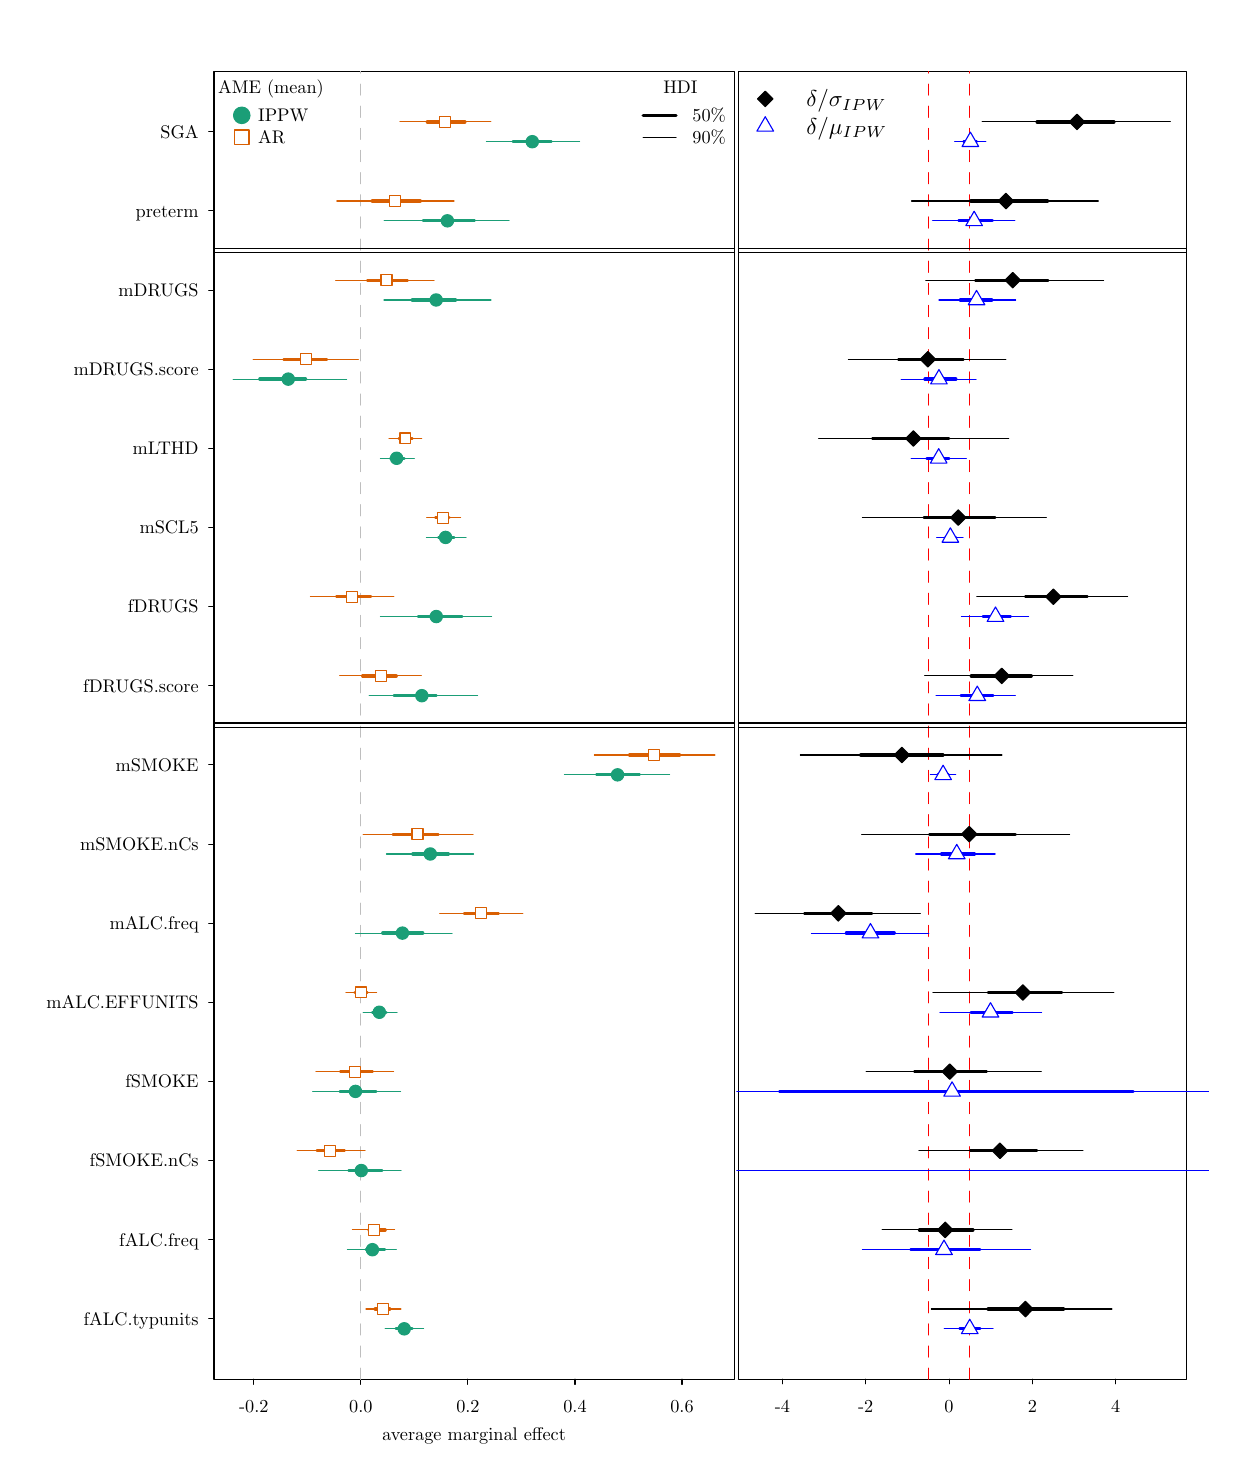
\begin{tikzpicture}[x=1pt,y=1pt]
\definecolor{fillColor}{RGB}{255,255,255}
\path[use as bounding box,fill=fillColor,fill opacity=0.00] (0,0) rectangle (426.79,512.15);
\begin{scope}
\path[clip] (  0.00,  0.00) rectangle (426.79,512.15);
\definecolor{drawColor}{RGB}{0,0,0}

\path[draw=drawColor,line width= 0.4pt,line join=round,line cap=round] ( 81.73, 23.76) -- (236.45, 23.76);

\path[draw=drawColor,line width= 0.4pt,line join=round,line cap=round] ( 81.73, 23.76) -- ( 81.73, 21.88);

\path[draw=drawColor,line width= 0.4pt,line join=round,line cap=round] (120.41, 23.76) -- (120.41, 21.88);

\path[draw=drawColor,line width= 0.4pt,line join=round,line cap=round] (159.09, 23.76) -- (159.09, 21.88);

\path[draw=drawColor,line width= 0.4pt,line join=round,line cap=round] (197.77, 23.76) -- (197.77, 21.88);

\path[draw=drawColor,line width= 0.4pt,line join=round,line cap=round] (236.45, 23.76) -- (236.45, 21.88);

\node[text=drawColor,anchor=base,inner sep=0pt, outer sep=0pt, scale=  0.66] at ( 81.73, 11.88) {-0.2};

\node[text=drawColor,anchor=base,inner sep=0pt, outer sep=0pt, scale=  0.66] at (120.41, 11.88) {0.0};

\node[text=drawColor,anchor=base,inner sep=0pt, outer sep=0pt, scale=  0.66] at (159.09, 11.88) {0.2};

\node[text=drawColor,anchor=base,inner sep=0pt, outer sep=0pt, scale=  0.66] at (197.77, 11.88) {0.4};

\node[text=drawColor,anchor=base,inner sep=0pt, outer sep=0pt, scale=  0.66] at (236.45, 11.88) {0.6};

\path[draw=drawColor,line width= 0.4pt,line join=round,line cap=round] ( 67.32, 23.76) --
	(255.28, 23.76) --
	(255.28,496.31) --
	( 67.32,496.31) --
	( 67.32, 23.76);
\end{scope}
\begin{scope}
\path[clip] (  0.00,  0.00) rectangle (256.07,512.15);
\definecolor{drawColor}{RGB}{0,0,0}

\node[text=drawColor,anchor=base,inner sep=0pt, outer sep=0pt, scale=  0.66] at (161.30,  1.58) {average marginal effect};
\end{scope}
\begin{scope}
\path[clip] ( 67.32, 23.76) rectangle (255.28,496.31);
\definecolor{drawColor}{RGB}{190,190,190}

\path[draw=drawColor,line width= 0.4pt,dash pattern=on 4pt off 4pt ,line join=round,line cap=round] (120.41, 23.76) -- (120.41,496.31);
\definecolor{drawColor}{RGB}{27,158,119}

\path[draw=drawColor,line width= 1.2pt,line join=round,line cap=round] (175.33,470.94) -- (189.22,470.94);

\path[draw=drawColor,line width= 1.2pt,line join=round,line cap=round] (142.87,442.35) -- (161.46,442.35);

\path[draw=drawColor,line width= 1.2pt,line join=round,line cap=round] (138.95,413.75) -- (154.58,413.75);

\path[draw=drawColor,line width= 1.2pt,line join=round,line cap=round] ( 83.89,385.15) -- (100.40,385.15);

\path[draw=drawColor,line width= 1.2pt,line join=round,line cap=round] (131.05,356.55) -- (136.06,356.55);

\path[draw=drawColor,line width= 1.2pt,line join=round,line cap=round] (148.43,327.95) -- (154.09,327.95);

\path[draw=drawColor,line width= 1.2pt,line join=round,line cap=round] (141.09,299.36) -- (156.98,299.36);

\path[draw=drawColor,line width= 1.2pt,line join=round,line cap=round] (132.35,270.76) -- (147.68,270.76);

\path[draw=drawColor,line width= 1.2pt,line join=round,line cap=round] (205.51,242.16) -- (221.12,242.16);

\path[draw=drawColor,line width= 1.2pt,line join=round,line cap=round] (139.19,213.56) -- (152.00,213.56);

\path[draw=drawColor,line width= 1.2pt,line join=round,line cap=round] (128.30,184.97) -- (142.75,184.97);

\path[draw=drawColor,line width= 1.2pt,line join=round,line cap=round] (124.54,156.37) -- (129.55,156.37);

\path[draw=drawColor,line width= 1.2pt,line join=round,line cap=round] (112.85,127.77) -- (125.88,127.77);

\path[draw=drawColor,line width= 1.2pt,line join=round,line cap=round] (116.00, 99.17) -- (128.07, 99.17);

\path[draw=drawColor,line width= 1.2pt,line join=round,line cap=round] (122.24, 70.57) -- (129.02, 70.57);

\path[draw=drawColor,line width= 1.2pt,line join=round,line cap=round] (133.09, 41.98) -- (138.95, 41.98);

\path[draw=drawColor,line width= 0.4pt,line join=round,line cap=round] (165.78,470.94) -- (199.46,470.94);

\path[draw=drawColor,line width= 0.4pt,line join=round,line cap=round] (128.81,442.35) -- (173.96,442.35);

\path[draw=drawColor,line width= 0.4pt,line join=round,line cap=round] (128.76,413.75) -- (167.41,413.75);

\path[draw=drawColor,line width= 0.4pt,line join=round,line cap=round] ( 74.28,385.15) -- (115.23,385.15);

\path[draw=drawColor,line width= 0.4pt,line join=round,line cap=round] (127.47,356.55) -- (139.76,356.55);

\path[draw=drawColor,line width= 0.4pt,line join=round,line cap=round] (144.12,327.95) -- (158.43,327.95);

\path[draw=drawColor,line width= 0.4pt,line join=round,line cap=round] (127.46,299.36) -- (167.62,299.36);

\path[draw=drawColor,line width= 0.4pt,line join=round,line cap=round] (123.42,270.76) -- (162.54,270.76);

\path[draw=drawColor,line width= 0.4pt,line join=round,line cap=round] (193.96,242.16) -- (231.99,242.16);

\path[draw=drawColor,line width= 0.4pt,line join=round,line cap=round] (129.64,213.56) -- (161.10,213.56);

\path[draw=drawColor,line width= 0.4pt,line join=round,line cap=round] (118.46,184.97) -- (153.33,184.97);

\path[draw=drawColor,line width= 0.4pt,line join=round,line cap=round] (121.20,156.37) -- (133.47,156.37);

\path[draw=drawColor,line width= 0.4pt,line join=round,line cap=round] (102.98,127.77) -- (134.74,127.77);

\path[draw=drawColor,line width= 0.4pt,line join=round,line cap=round] (105.17, 99.17) -- (134.93, 99.17);

\path[draw=drawColor,line width= 0.4pt,line join=round,line cap=round] (115.51, 70.57) -- (133.20, 70.57);

\path[draw=drawColor,line width= 0.4pt,line join=round,line cap=round] (129.17, 41.98) -- (143.08, 41.98);
\definecolor{fillColor}{RGB}{27,158,119}

\path[draw=drawColor,line width= 0.4pt,line join=round,line cap=round,fill=fillColor] (182.34,470.94) circle (  2.23);

\path[draw=drawColor,line width= 0.4pt,line join=round,line cap=round,fill=fillColor] (151.67,442.35) circle (  2.23);

\path[draw=drawColor,line width= 0.4pt,line join=round,line cap=round,fill=fillColor] (147.61,413.75) circle (  2.23);

\path[draw=drawColor,line width= 0.4pt,line join=round,line cap=round,fill=fillColor] ( 94.16,385.15) circle (  2.23);

\path[draw=drawColor,line width= 0.4pt,line join=round,line cap=round,fill=fillColor] (133.31,356.55) circle (  2.23);

\path[draw=drawColor,line width= 0.4pt,line join=round,line cap=round,fill=fillColor] (151.01,327.95) circle (  2.23);

\path[draw=drawColor,line width= 0.4pt,line join=round,line cap=round,fill=fillColor] (147.64,299.36) circle (  2.23);

\path[draw=drawColor,line width= 0.4pt,line join=round,line cap=round,fill=fillColor] (142.43,270.76) circle (  2.23);

\path[draw=drawColor,line width= 0.4pt,line join=round,line cap=round,fill=fillColor] (213.15,242.16) circle (  2.23);

\path[draw=drawColor,line width= 0.4pt,line join=round,line cap=round,fill=fillColor] (145.48,213.56) circle (  2.23);

\path[draw=drawColor,line width= 0.4pt,line join=round,line cap=round,fill=fillColor] (135.42,184.97) circle (  2.23);

\path[draw=drawColor,line width= 0.4pt,line join=round,line cap=round,fill=fillColor] (127.07,156.37) circle (  2.23);

\path[draw=drawColor,line width= 0.4pt,line join=round,line cap=round,fill=fillColor] (118.44,127.77) circle (  2.23);

\path[draw=drawColor,line width= 0.4pt,line join=round,line cap=round,fill=fillColor] (120.56, 99.17) circle (  2.23);

\path[draw=drawColor,line width= 0.4pt,line join=round,line cap=round,fill=fillColor] (124.57, 70.57) circle (  2.23);

\path[draw=drawColor,line width= 0.4pt,line join=round,line cap=round,fill=fillColor] (136.07, 41.98) circle (  2.23);
\definecolor{drawColor}{RGB}{217,95,2}

\path[draw=drawColor,line width= 1.2pt,line join=round,line cap=round] (144.42,478.09) -- (157.97,478.09);

\path[draw=drawColor,line width= 1.2pt,line join=round,line cap=round] (124.49,449.50) -- (141.84,449.50);

\path[draw=drawColor,line width= 1.2pt,line join=round,line cap=round] (122.73,420.90) -- (137.26,420.90);

\path[draw=drawColor,line width= 1.2pt,line join=round,line cap=round] ( 92.52,392.30) -- (108.08,392.30);

\path[draw=drawColor,line width= 1.2pt,line join=round,line cap=round] (134.16,363.70) -- (138.97,363.70);

\path[draw=drawColor,line width= 1.2pt,line join=round,line cap=round] (147.35,335.10) -- (152.31,335.10);

\path[draw=drawColor,line width= 1.2pt,line join=round,line cap=round] (111.54,306.51) -- (124.03,306.51);

\path[draw=drawColor,line width= 1.2pt,line join=round,line cap=round] (121.04,277.91) -- (133.17,277.91);

\path[draw=drawColor,line width= 1.2pt,line join=round,line cap=round] (217.51,249.31) -- (235.54,249.31);

\path[draw=drawColor,line width= 1.2pt,line join=round,line cap=round] (131.96,220.71) -- (148.38,220.71);

\path[draw=drawColor,line width= 1.2pt,line join=round,line cap=round] (157.74,192.12) -- (170.18,192.12);

\path[draw=drawColor,line width= 1.2pt,line join=round,line cap=round] (118.21,163.52) -- (122.75,163.52);

\path[draw=drawColor,line width= 1.2pt,line join=round,line cap=round] (112.98,134.92) -- (124.62,134.92);

\path[draw=drawColor,line width= 1.2pt,line join=round,line cap=round] (104.50,106.32) -- (114.48,106.32);

\path[draw=drawColor,line width= 1.2pt,line join=round,line cap=round] (123.36, 77.72) -- (129.17, 77.72);

\path[draw=drawColor,line width= 1.2pt,line join=round,line cap=round] (125.57, 49.13) -- (130.80, 49.13);

\path[draw=drawColor,line width= 0.4pt,line join=round,line cap=round] (134.51,478.09) -- (167.37,478.09);

\path[draw=drawColor,line width= 0.4pt,line join=round,line cap=round] (111.72,449.50) -- (154.06,449.50);

\path[draw=drawColor,line width= 0.4pt,line join=round,line cap=round] (111.26,420.90) -- (146.87,420.90);

\path[draw=drawColor,line width= 0.4pt,line join=round,line cap=round] ( 81.47,392.30) -- (119.49,392.30);

\path[draw=drawColor,line width= 0.4pt,line join=round,line cap=round] (130.57,363.70) -- (142.38,363.70);

\path[draw=drawColor,line width= 0.4pt,line join=round,line cap=round] (144.16,335.10) -- (156.44,335.10);

\path[draw=drawColor,line width= 0.4pt,line join=round,line cap=round] (102.16,306.51) -- (132.30,306.51);

\path[draw=drawColor,line width= 0.4pt,line join=round,line cap=round] (112.72,277.91) -- (142.22,277.91);

\path[draw=drawColor,line width= 0.4pt,line join=round,line cap=round] (204.77,249.31) -- (248.32,249.31);

\path[draw=drawColor,line width= 0.4pt,line join=round,line cap=round] (121.26,220.71) -- (160.95,220.71);

\path[draw=drawColor,line width= 0.4pt,line join=round,line cap=round] (148.87,192.12) -- (178.91,192.12);

\path[draw=drawColor,line width= 0.4pt,line join=round,line cap=round] (114.98,163.52) -- (126.07,163.52);

\path[draw=drawColor,line width= 0.4pt,line join=round,line cap=round] (104.12,134.92) -- (132.21,134.92);

\path[draw=drawColor,line width= 0.4pt,line join=round,line cap=round] ( 97.41,106.32) -- (121.89,106.32);

\path[draw=drawColor,line width= 0.4pt,line join=round,line cap=round] (117.36, 77.72) -- (132.56, 77.72);

\path[draw=drawColor,line width= 0.4pt,line join=round,line cap=round] (122.25, 49.13) -- (134.87, 49.13);
\definecolor{fillColor}{RGB}{255,255,255}

\path[draw=drawColor,line width= 0.4pt,line join=round,line cap=round,fill=fillColor] (148.70,476.12) rectangle (152.65,480.07);

\path[draw=drawColor,line width= 0.4pt,line join=round,line cap=round,fill=fillColor] (130.88,447.52) rectangle (134.83,451.47);

\path[draw=drawColor,line width= 0.4pt,line join=round,line cap=round,fill=fillColor] (127.69,418.92) rectangle (131.64,422.87);

\path[draw=drawColor,line width= 0.4pt,line join=round,line cap=round,fill=fillColor] ( 98.54,390.33) rectangle (102.49,394.27);

\path[draw=drawColor,line width= 0.4pt,line join=round,line cap=round,fill=fillColor] (134.54,361.73) rectangle (138.49,365.68);

\path[draw=drawColor,line width= 0.4pt,line join=round,line cap=round,fill=fillColor] (148.07,333.13) rectangle (152.02,337.08);

\path[draw=drawColor,line width= 0.4pt,line join=round,line cap=round,fill=fillColor] (115.31,304.53) rectangle (119.26,308.48);

\path[draw=drawColor,line width= 0.4pt,line join=round,line cap=round,fill=fillColor] (125.55,275.93) rectangle (129.50,279.88);

\path[draw=drawColor,line width= 0.4pt,line join=round,line cap=round,fill=fillColor] (224.38,247.34) rectangle (228.33,251.28);

\path[draw=drawColor,line width= 0.4pt,line join=round,line cap=round,fill=fillColor] (138.88,218.74) rectangle (142.83,222.69);

\path[draw=drawColor,line width= 0.4pt,line join=round,line cap=round,fill=fillColor] (161.75,190.14) rectangle (165.70,194.09);

\path[draw=drawColor,line width= 0.4pt,line join=round,line cap=round,fill=fillColor] (118.47,161.54) rectangle (122.42,165.49);

\path[draw=drawColor,line width= 0.4pt,line join=round,line cap=round,fill=fillColor] (116.32,132.95) rectangle (120.27,136.89);

\path[draw=drawColor,line width= 0.4pt,line join=round,line cap=round,fill=fillColor] (107.23,104.35) rectangle (111.18,108.30);

\path[draw=drawColor,line width= 0.4pt,line join=round,line cap=round,fill=fillColor] (123.10, 75.75) rectangle (127.05, 79.70);

\path[draw=drawColor,line width= 0.4pt,line join=round,line cap=round,fill=fillColor] (126.32, 47.15) rectangle (130.27, 51.10);
\end{scope}
\begin{scope}
\path[clip] (  0.00,  0.00) rectangle (426.79,512.15);
\definecolor{drawColor}{RGB}{0,0,0}

\path[draw=drawColor,line width= 0.4pt,line join=round,line cap=round] ( 67.32, 45.55) -- ( 67.32,474.52);

\path[draw=drawColor,line width= 0.4pt,line join=round,line cap=round] ( 67.32, 45.55) -- ( 65.44, 45.55);

\path[draw=drawColor,line width= 0.4pt,line join=round,line cap=round] ( 67.32, 74.15) -- ( 65.44, 74.15);

\path[draw=drawColor,line width= 0.4pt,line join=round,line cap=round] ( 67.32,102.75) -- ( 65.44,102.75);

\path[draw=drawColor,line width= 0.4pt,line join=round,line cap=round] ( 67.32,131.34) -- ( 65.44,131.34);

\path[draw=drawColor,line width= 0.4pt,line join=round,line cap=round] ( 67.32,159.94) -- ( 65.44,159.94);

\path[draw=drawColor,line width= 0.4pt,line join=round,line cap=round] ( 67.32,188.54) -- ( 65.44,188.54);

\path[draw=drawColor,line width= 0.4pt,line join=round,line cap=round] ( 67.32,217.14) -- ( 65.44,217.14);

\path[draw=drawColor,line width= 0.4pt,line join=round,line cap=round] ( 67.32,245.74) -- ( 65.44,245.74);

\path[draw=drawColor,line width= 0.4pt,line join=round,line cap=round] ( 67.32,274.33) -- ( 65.44,274.33);

\path[draw=drawColor,line width= 0.4pt,line join=round,line cap=round] ( 67.32,302.93) -- ( 65.44,302.93);

\path[draw=drawColor,line width= 0.4pt,line join=round,line cap=round] ( 67.32,331.53) -- ( 65.44,331.53);

\path[draw=drawColor,line width= 0.4pt,line join=round,line cap=round] ( 67.32,360.13) -- ( 65.44,360.13);

\path[draw=drawColor,line width= 0.4pt,line join=round,line cap=round] ( 67.32,388.72) -- ( 65.44,388.72);

\path[draw=drawColor,line width= 0.4pt,line join=round,line cap=round] ( 67.32,417.32) -- ( 65.44,417.32);

\path[draw=drawColor,line width= 0.4pt,line join=round,line cap=round] ( 67.32,445.92) -- ( 65.44,445.92);

\path[draw=drawColor,line width= 0.4pt,line join=round,line cap=round] ( 67.32,474.52) -- ( 65.44,474.52);

\node[text=drawColor,anchor=base east,inner sep=0pt, outer sep=0pt, scale=  0.66] at ( 61.78, 43.28) {fALC.typunits};

\node[text=drawColor,anchor=base east,inner sep=0pt, outer sep=0pt, scale=  0.66] at ( 61.78, 71.88) {fALC.freq};

\node[text=drawColor,anchor=base east,inner sep=0pt, outer sep=0pt, scale=  0.66] at ( 61.78,100.47) {fSMOKE.nCs};

\node[text=drawColor,anchor=base east,inner sep=0pt, outer sep=0pt, scale=  0.66] at ( 61.78,129.07) {fSMOKE};

\node[text=drawColor,anchor=base east,inner sep=0pt, outer sep=0pt, scale=  0.66] at ( 61.78,157.67) {mALC.EFFUNITS};

\node[text=drawColor,anchor=base east,inner sep=0pt, outer sep=0pt, scale=  0.66] at ( 61.78,186.27) {mALC.freq};

\node[text=drawColor,anchor=base east,inner sep=0pt, outer sep=0pt, scale=  0.66] at ( 61.78,214.87) {mSMOKE.nCs};

\node[text=drawColor,anchor=base east,inner sep=0pt, outer sep=0pt, scale=  0.66] at ( 61.78,243.46) {mSMOKE};

\node[text=drawColor,anchor=base east,inner sep=0pt, outer sep=0pt, scale=  0.66] at ( 61.78,272.06) {fDRUGS.score};

\node[text=drawColor,anchor=base east,inner sep=0pt, outer sep=0pt, scale=  0.66] at ( 61.78,300.66) {fDRUGS};

\node[text=drawColor,anchor=base east,inner sep=0pt, outer sep=0pt, scale=  0.66] at ( 61.78,329.26) {mSCL5};

\node[text=drawColor,anchor=base east,inner sep=0pt, outer sep=0pt, scale=  0.66] at ( 61.78,357.85) {mLTHD};

\node[text=drawColor,anchor=base east,inner sep=0pt, outer sep=0pt, scale=  0.66] at ( 61.78,386.45) {mDRUGS.score};

\node[text=drawColor,anchor=base east,inner sep=0pt, outer sep=0pt, scale=  0.66] at ( 61.78,415.05) {mDRUGS};

\node[text=drawColor,anchor=base east,inner sep=0pt, outer sep=0pt, scale=  0.66] at ( 61.78,443.65) {preterm};

\node[text=drawColor,anchor=base east,inner sep=0pt, outer sep=0pt, scale=  0.66] at ( 61.78,472.25) {SGA};
\end{scope}
\begin{scope}
\path[clip] ( 67.32, 23.76) rectangle (255.28,496.31);
\definecolor{drawColor}{RGB}{27,158,119}
\definecolor{fillColor}{RGB}{27,158,119}

\path[draw=drawColor,line width= 0.4pt,line join=round,line cap=round,fill=fillColor] ( 77.36,480.47) circle (  2.97);
\definecolor{drawColor}{RGB}{217,95,2}
\definecolor{fillColor}{RGB}{255,255,255}

\path[draw=drawColor,line width= 0.4pt,line join=round,line cap=round,fill=fillColor] ( 74.72,469.92) rectangle ( 79.99,475.18);
\definecolor{drawColor}{RGB}{0,0,0}

\node[text=drawColor,anchor=base,inner sep=0pt, outer sep=0pt, scale=  0.66] at ( 87.91,488.39) {AME (mean)};

\node[text=drawColor,anchor=base west,inner sep=0pt, outer sep=0pt, scale=  0.66] at ( 83.30,478.20) {IPPW};

\node[text=drawColor,anchor=base west,inner sep=0pt, outer sep=0pt, scale=  0.66] at ( 83.30,470.28) {AR};

\path[draw=drawColor,line width= 1.2pt,line join=round,line cap=round] (222.40,480.47) -- (234.28,480.47);

\path[draw=drawColor,line width= 0.4pt,line join=round,line cap=round] (222.40,472.55) -- (234.28,472.55);

\node[text=drawColor,anchor=base,inner sep=0pt, outer sep=0pt, scale=  0.66] at (235.87,488.39) {HDI};

\node[text=drawColor,anchor=base west,inner sep=0pt, outer sep=0pt, scale=  0.66] at (240.22,478.20) {50\%};

\node[text=drawColor,anchor=base west,inner sep=0pt, outer sep=0pt, scale=  0.66] at (240.22,470.28) {90\%};

\path[draw=drawColor,line width= 0.4pt,line join=round,line cap=round] ( 67.32,430.76) -- (255.28,430.76);

\path[draw=drawColor,line width= 0.4pt,line join=round,line cap=round] ( 67.32,432.48) -- (255.28,432.48);

\path[draw=drawColor,line width= 0.4pt,line join=round,line cap=round] ( 67.32,259.18) -- (255.28,259.18);

\path[draw=drawColor,line width= 0.4pt,line join=round,line cap=round] ( 67.32,260.89) -- (255.28,260.89);
\end{scope}
\begin{scope}
\path[clip] (  0.00,  0.00) rectangle (426.79,512.15);
\definecolor{drawColor}{RGB}{0,0,0}

\path[draw=drawColor,line width= 0.4pt,line join=round,line cap=round] (272.72, 23.76) -- (393.15, 23.76);

\path[draw=drawColor,line width= 0.4pt,line join=round,line cap=round] (272.72, 23.76) -- (272.72, 22.14);

\path[draw=drawColor,line width= 0.4pt,line join=round,line cap=round] (302.83, 23.76) -- (302.83, 22.14);

\path[draw=drawColor,line width= 0.4pt,line join=round,line cap=round] (332.94, 23.76) -- (332.94, 22.14);

\path[draw=drawColor,line width= 0.4pt,line join=round,line cap=round] (363.05, 23.76) -- (363.05, 22.14);

\path[draw=drawColor,line width= 0.4pt,line join=round,line cap=round] (393.15, 23.76) -- (393.15, 22.14);

\node[text=drawColor,anchor=base,inner sep=0pt, outer sep=0pt, scale=  0.66] at (272.72, 11.88) {-4};

\node[text=drawColor,anchor=base,inner sep=0pt, outer sep=0pt, scale=  0.66] at (302.83, 11.88) {-2};

\node[text=drawColor,anchor=base,inner sep=0pt, outer sep=0pt, scale=  0.66] at (332.94, 11.88) {0};

\node[text=drawColor,anchor=base,inner sep=0pt, outer sep=0pt, scale=  0.66] at (363.05, 11.88) {2};

\node[text=drawColor,anchor=base,inner sep=0pt, outer sep=0pt, scale=  0.66] at (393.15, 11.88) {4};

\path[draw=drawColor,line width= 0.4pt,line join=round,line cap=round] (256.87, 23.76) --
	(418.87, 23.76) --
	(418.87,496.31) --
	(256.87,496.31) --
	(256.87, 23.76);
\end{scope}
\begin{scope}
\path[clip] (256.87, 23.76) rectangle (418.87,496.31);
\definecolor{drawColor}{RGB}{255,0,0}

\path[draw=drawColor,line width= 0.4pt,dash pattern=on 4pt off 4pt ,line join=round,line cap=round] (325.41, 23.76) -- (325.41,496.31);

\path[draw=drawColor,line width= 0.4pt,dash pattern=on 4pt off 4pt ,line join=round,line cap=round] (340.47, 23.76) -- (340.47,496.31);
\end{scope}
\begin{scope}
\path[clip] (256.07,  0.00) rectangle (426.79,512.15);
\definecolor{drawColor}{RGB}{0,0,0}

\path[draw=drawColor,line width= 0.4pt,line join=round,line cap=round] (344.92,478.09) -- (412.87,478.09);

\path[draw=drawColor,line width= 0.4pt,line join=round,line cap=round] (319.39,449.50) -- (386.85,449.50);

\path[draw=drawColor,line width= 0.4pt,line join=round,line cap=round] (324.53,420.90) -- (388.76,420.90);

\path[draw=drawColor,line width= 0.4pt,line join=round,line cap=round] (296.54,392.30) -- (353.45,392.30);

\path[draw=drawColor,line width= 0.4pt,line join=round,line cap=round] (285.78,363.70) -- (354.49,363.70);

\path[draw=drawColor,line width= 0.4pt,line join=round,line cap=round] (301.63,335.10) -- (368.09,335.10);

\path[draw=drawColor,line width= 0.4pt,line join=round,line cap=round] (342.96,306.51) -- (397.47,306.51);

\path[draw=drawColor,line width= 0.4pt,line join=round,line cap=round] (324.16,277.91) -- (377.63,277.91);

\path[draw=drawColor,line width= 0.4pt,line join=round,line cap=round] (279.20,249.31) -- (352.04,249.31);

\path[draw=drawColor,line width= 0.4pt,line join=round,line cap=round] (301.38,220.71) -- (376.52,220.71);

\path[draw=drawColor,line width= 0.4pt,line join=round,line cap=round] (262.87,192.12) -- (322.58,192.12);

\path[draw=drawColor,line width= 0.4pt,line join=round,line cap=round] (327.08,163.52) -- (392.47,163.52);

\path[draw=drawColor,line width= 0.4pt,line join=round,line cap=round] (303.00,134.92) -- (366.24,134.92);

\path[draw=drawColor,line width= 0.4pt,line join=round,line cap=round] (322.05,106.32) -- (381.32,106.32);

\path[draw=drawColor,line width= 0.4pt,line join=round,line cap=round] (308.74, 77.72) -- (355.67, 77.72);

\path[draw=drawColor,line width= 0.4pt,line join=round,line cap=round] (326.55, 49.13) -- (391.78, 49.13);

\path[draw=drawColor,line width= 1.2pt,line join=round,line cap=round] (364.77,478.09) -- (392.50,478.09);

\path[draw=drawColor,line width= 1.2pt,line join=round,line cap=round] (340.80,449.50) -- (368.51,449.50);

\path[draw=drawColor,line width= 1.2pt,line join=round,line cap=round] (342.45,420.90) -- (368.72,420.90);

\path[draw=drawColor,line width= 1.2pt,line join=round,line cap=round] (314.62,392.30) -- (338.08,392.30);

\path[draw=drawColor,line width= 1.2pt,line join=round,line cap=round] (305.25,363.70) -- (332.89,363.70);

\path[draw=drawColor,line width= 1.2pt,line join=round,line cap=round] (323.86,335.10) -- (349.56,335.10);

\path[draw=drawColor,line width= 1.2pt,line join=round,line cap=round] (360.50,306.51) -- (382.92,306.51);

\path[draw=drawColor,line width= 1.2pt,line join=round,line cap=round] (340.98,277.91) -- (362.62,277.91);

\path[draw=drawColor,line width= 1.2pt,line join=round,line cap=round] (301.02,249.31) -- (330.72,249.31);

\path[draw=drawColor,line width= 1.2pt,line join=round,line cap=round] (325.88,220.71) -- (356.93,220.71);

\path[draw=drawColor,line width= 1.2pt,line join=round,line cap=round] (280.68,192.12) -- (305.02,192.12);

\path[draw=drawColor,line width= 1.2pt,line join=round,line cap=round] (347.04,163.52) -- (373.65,163.52);

\path[draw=drawColor,line width= 1.2pt,line join=round,line cap=round] (320.45,134.92) -- (346.49,134.92);

\path[draw=drawColor,line width= 1.2pt,line join=round,line cap=round] (340.67,106.32) -- (364.64,106.32);

\path[draw=drawColor,line width= 1.2pt,line join=round,line cap=round] (322.25, 77.72) -- (341.55, 77.72);

\path[draw=drawColor,line width= 1.2pt,line join=round,line cap=round] (347.07, 49.13) -- (374.29, 49.13);
\definecolor{drawColor}{RGB}{0,0,255}

\path[draw=drawColor,line width= 0.4pt,line join=round,line cap=round] (334.93,470.94) -- (346.26,470.94);

\path[draw=drawColor,line width= 0.4pt,line join=round,line cap=round] (326.97,442.35) -- (356.70,442.35);

\path[draw=drawColor,line width= 0.4pt,line join=round,line cap=round] (329.31,413.75) -- (357.01,413.75);

\path[draw=drawColor,line width= 0.4pt,line join=round,line cap=round] (315.63,385.15) -- (342.69,385.15);

\path[draw=drawColor,line width= 0.4pt,line join=round,line cap=round] (319.23,356.55) -- (339.20,356.55);

\path[draw=drawColor,line width= 0.4pt,line join=round,line cap=round] (328.42,327.95) -- (338.01,327.95);

\path[draw=drawColor,line width= 0.4pt,line join=round,line cap=round] (337.40,299.36) -- (361.67,299.36);

\path[draw=drawColor,line width= 0.4pt,line join=round,line cap=round] (328.23,270.76) -- (356.87,270.76);

\path[draw=drawColor,line width= 0.4pt,line join=round,line cap=round] (326.19,242.16) -- (335.34,242.16);

\path[draw=drawColor,line width= 0.4pt,line join=round,line cap=round] (320.89,213.56) -- (349.58,213.56);

\path[draw=drawColor,line width= 0.4pt,line join=round,line cap=round] (283.21,184.97) -- (325.59,184.97);

\path[draw=drawColor,line width= 0.4pt,line join=round,line cap=round] (329.65,156.37) -- (366.36,156.37);

\path[draw=drawColor,line width= 0.4pt,line join=round,line cap=round] (185.92,127.77) -- (426.79,127.77);

\path[draw=drawColor,line width= 0.4pt,line join=round,line cap=round] (  0.00, 99.17) -- (426.79, 99.17);

\path[draw=drawColor,line width= 0.4pt,line join=round,line cap=round] (301.59, 70.57) -- (362.39, 70.57);

\path[draw=drawColor,line width= 0.4pt,line join=round,line cap=round] (331.21, 41.98) -- (348.87, 41.98);

\path[draw=drawColor,line width= 1.2pt,line join=round,line cap=round] (338.24,470.94) -- (342.86,470.94);

\path[draw=drawColor,line width= 1.2pt,line join=round,line cap=round] (336.40,442.35) -- (348.62,442.35);

\path[draw=drawColor,line width= 1.2pt,line join=round,line cap=round] (337.04,413.75) -- (348.37,413.75);

\path[draw=drawColor,line width= 1.2pt,line join=round,line cap=round] (324.23,385.15) -- (335.38,385.15);

\path[draw=drawColor,line width= 1.2pt,line join=round,line cap=round] (324.89,356.55) -- (332.92,356.55);

\path[draw=drawColor,line width= 1.2pt,line join=round,line cap=round] (331.63,327.95) -- (335.34,327.95);

\path[draw=drawColor,line width= 1.2pt,line join=round,line cap=round] (345.21,299.36) -- (355.19,299.36);

\path[draw=drawColor,line width= 1.2pt,line join=round,line cap=round] (337.25,270.76) -- (348.83,270.76);

\path[draw=drawColor,line width= 1.2pt,line join=round,line cap=round] (328.93,242.16) -- (332.66,242.16);

\path[draw=drawColor,line width= 1.2pt,line join=round,line cap=round] (330.24,213.56) -- (342.10,213.56);

\path[draw=drawColor,line width= 1.2pt,line join=round,line cap=round] (295.85,184.97) -- (313.13,184.97);

\path[draw=drawColor,line width= 1.2pt,line join=round,line cap=round] (340.85,156.37) -- (355.79,156.37);

\path[draw=drawColor,line width= 1.2pt,line join=round,line cap=round] (271.62,127.77) -- (399.48,127.77);

\path[draw=drawColor,line width= 1.2pt,line join=round,line cap=round] (319.10, 70.57) -- (344.10, 70.57);

\path[draw=drawColor,line width= 1.2pt,line join=round,line cap=round] (336.77, 41.98) -- (344.13, 41.98);
\definecolor{drawColor}{RGB}{0,0,0}
\definecolor{fillColor}{RGB}{0,0,0}

\path[draw=drawColor,line width= 0.4pt,line join=round,line cap=round,fill=fillColor] (379.14,475.30) --
	(381.93,478.09) --
	(379.14,480.88) --
	(376.35,478.09) --
	cycle;

\path[draw=drawColor,line width= 0.4pt,line join=round,line cap=round,fill=fillColor] (353.50,446.70) --
	(356.29,449.50) --
	(353.50,452.29) --
	(350.71,449.50) --
	cycle;

\path[draw=drawColor,line width= 0.4pt,line join=round,line cap=round,fill=fillColor] (355.97,418.11) --
	(358.76,420.90) --
	(355.97,423.69) --
	(353.18,420.90) --
	cycle;

\path[draw=drawColor,line width= 0.4pt,line join=round,line cap=round,fill=fillColor] (325.28,389.51) --
	(328.07,392.30) --
	(325.28,395.09) --
	(322.48,392.30) --
	cycle;

\path[draw=drawColor,line width= 0.4pt,line join=round,line cap=round,fill=fillColor] (320.08,360.91) --
	(322.87,363.70) --
	(320.08,366.49) --
	(317.29,363.70) --
	cycle;

\path[draw=drawColor,line width= 0.4pt,line join=round,line cap=round,fill=fillColor] (336.23,332.31) --
	(339.02,335.10) --
	(336.23,337.90) --
	(333.44,335.10) --
	cycle;

\path[draw=drawColor,line width= 0.4pt,line join=round,line cap=round,fill=fillColor] (370.63,303.71) --
	(373.43,306.51) --
	(370.63,309.30) --
	(367.84,306.51) --
	cycle;

\path[draw=drawColor,line width= 0.4pt,line join=round,line cap=round,fill=fillColor] (351.96,275.12) --
	(354.75,277.91) --
	(351.96,280.70) --
	(349.17,277.91) --
	cycle;

\path[draw=drawColor,line width= 0.4pt,line join=round,line cap=round,fill=fillColor] (315.87,246.52) --
	(318.66,249.31) --
	(315.87,252.10) --
	(313.08,249.31) --
	cycle;

\path[draw=drawColor,line width= 0.4pt,line join=round,line cap=round,fill=fillColor] (340.22,217.92) --
	(343.01,220.71) --
	(340.22,223.50) --
	(337.43,220.71) --
	cycle;

\path[draw=drawColor,line width= 0.4pt,line join=round,line cap=round,fill=fillColor] (292.93,189.32) --
	(295.72,192.12) --
	(292.93,194.91) --
	(290.14,192.12) --
	cycle;

\path[draw=drawColor,line width= 0.4pt,line join=round,line cap=round,fill=fillColor] (359.62,160.73) --
	(362.41,163.52) --
	(359.62,166.31) --
	(356.82,163.52) --
	cycle;

\path[draw=drawColor,line width= 0.4pt,line join=round,line cap=round,fill=fillColor] (333.16,132.13) --
	(335.95,134.92) --
	(333.16,137.71) --
	(330.37,134.92) --
	cycle;

\path[draw=drawColor,line width= 0.4pt,line join=round,line cap=round,fill=fillColor] (351.34,103.53) --
	(354.13,106.32) --
	(351.34,109.11) --
	(348.55,106.32) --
	cycle;

\path[draw=drawColor,line width= 0.4pt,line join=round,line cap=round,fill=fillColor] (331.53, 74.93) --
	(334.32, 77.72) --
	(331.53, 80.52) --
	(328.74, 77.72) --
	cycle;

\path[draw=drawColor,line width= 0.4pt,line join=round,line cap=round,fill=fillColor] (360.54, 46.33) --
	(363.33, 49.13) --
	(360.54, 51.92) --
	(357.75, 49.13) --
	cycle;
\definecolor{drawColor}{RGB}{0,0,255}
\definecolor{fillColor}{RGB}{255,255,255}

\path[draw=drawColor,line width= 0.4pt,line join=round,line cap=round,fill=fillColor] (340.64,474.41) --
	(343.64,469.21) --
	(337.64,469.21) --
	cycle;

\path[draw=drawColor,line width= 0.4pt,line join=round,line cap=round,fill=fillColor] (342.00,445.81) --
	(345.00,440.61) --
	(339.00,440.61) --
	cycle;

\path[draw=drawColor,line width= 0.4pt,line join=round,line cap=round,fill=fillColor] (342.87,417.21) --
	(345.87,412.02) --
	(339.87,412.02) --
	cycle;

\path[draw=drawColor,line width= 0.4pt,line join=round,line cap=round,fill=fillColor] (329.29,388.61) --
	(332.29,383.42) --
	(326.29,383.42) --
	cycle;

\path[draw=drawColor,line width= 0.4pt,line join=round,line cap=round,fill=fillColor] (329.20,360.02) --
	(332.20,354.82) --
	(326.20,354.82) --
	cycle;

\path[draw=drawColor,line width= 0.4pt,line join=round,line cap=round,fill=fillColor] (333.41,331.42) --
	(336.41,326.22) --
	(330.41,326.22) --
	cycle;

\path[draw=drawColor,line width= 0.4pt,line join=round,line cap=round,fill=fillColor] (349.72,302.82) --
	(352.72,297.62) --
	(346.72,297.62) --
	cycle;

\path[draw=drawColor,line width= 0.4pt,line join=round,line cap=round,fill=fillColor] (343.13,274.22) --
	(346.13,269.03) --
	(340.13,269.03) --
	cycle;

\path[draw=drawColor,line width= 0.4pt,line join=round,line cap=round,fill=fillColor] (330.79,245.63) --
	(333.79,240.43) --
	(327.79,240.43) --
	cycle;

\path[draw=drawColor,line width= 0.4pt,line join=round,line cap=round,fill=fillColor] (335.72,217.03) --
	(338.72,211.83) --
	(332.72,211.83) --
	cycle;

\path[draw=drawColor,line width= 0.4pt,line join=round,line cap=round,fill=fillColor] (304.54,188.43) --
	(307.54,183.23) --
	(301.54,183.23) --
	cycle;

\path[draw=drawColor,line width= 0.4pt,line join=round,line cap=round,fill=fillColor] (347.91,159.83) --
	(350.91,154.64) --
	(344.91,154.64) --
	cycle;

\path[draw=drawColor,line width= 0.4pt,line join=round,line cap=round,fill=fillColor] (334.03,131.23) --
	(337.03,126.04) --
	(331.03,126.04) --
	cycle;

\path[draw=drawColor,line width= 0.4pt,line join=round,line cap=round,fill=fillColor] (331.11, 74.04) --
	(334.11, 68.84) --
	(328.11, 68.84) --
	cycle;

\path[draw=drawColor,line width= 0.4pt,line join=round,line cap=round,fill=fillColor] (340.41, 45.44) --
	(343.41, 40.24) --
	(337.41, 40.24) --
	cycle;
\definecolor{drawColor}{RGB}{0,0,0}
\definecolor{fillColor}{RGB}{0,0,0}

\path[draw=drawColor,line width= 0.4pt,line join=round,line cap=round,fill=fillColor] (266.52,483.62) --
	(269.31,486.41) --
	(266.52,489.20) --
	(263.73,486.41) --
	cycle;
\definecolor{drawColor}{RGB}{0,0,255}
\definecolor{fillColor}{RGB}{255,255,255}

\path[draw=drawColor,line width= 0.4pt,line join=round,line cap=round,fill=fillColor] (266.52,479.97) --
	(269.52,474.78) --
	(263.52,474.78) --
	cycle;
\definecolor{drawColor}{RGB}{0,0,0}

\node[text=drawColor,anchor=base west,inner sep=0pt, outer sep=0pt, scale=  0.83] at (281.37,483.57) {$\delta/\sigma_{IPW}$};

\node[text=drawColor,anchor=base west,inner sep=0pt, outer sep=0pt, scale=  0.83] at (281.37,473.67) {$\delta/\mu_{IPW}$};
\end{scope}
\begin{scope}
\path[clip] (256.87, 23.76) rectangle (418.87,496.31);
\definecolor{drawColor}{RGB}{0,0,0}

\path[draw=drawColor,line width= 0.4pt,line join=round,line cap=round] (256.87,430.76) -- (418.87,430.76);

\path[draw=drawColor,line width= 0.4pt,line join=round,line cap=round] (256.87,432.48) -- (418.87,432.48);

\path[draw=drawColor,line width= 0.4pt,line join=round,line cap=round] (256.87,259.18) -- (418.87,259.18);

\path[draw=drawColor,line width= 0.4pt,line join=round,line cap=round] (256.87,260.89) -- (418.87,260.89);
\end{scope}
\end{tikzpicture}

	\caption{\footnotesize \linespread{1.3}\selectfont{} Exposure association estimates. AR: regression adjusted for participation indicators. IPW: inverse probability of participation weighted regression. The left panel shows association estimates in terms of average marginal effects ($AME$) of a one point increase of the exposure (all exposures except parity were standardized). HDI: Highest density interval of the posterior distribution. The right panel shows differences between the AR and IPW estimates ($\delta = AME_{IPW}-AME_{AR}$), standardized by the mean ($\mu_{IPW}$) or the standard deviation ($\sigma_{IPW}$) of the IPW estimates. To confirm the absence of bias, the 90\% HDI should fall within a region of negligible differences between the AR and IPWR estimates. The two red lines enclose a region where the deviation is smaller than 50\% of the mean or standard deviation of the IPW estimate.}
	\label{fig:estimates}
\end{figure}

% Created by tikzDevice version 0.11 on 2018-07-24 15:50:23
% !TEX encoding = UTF-8 Unicode
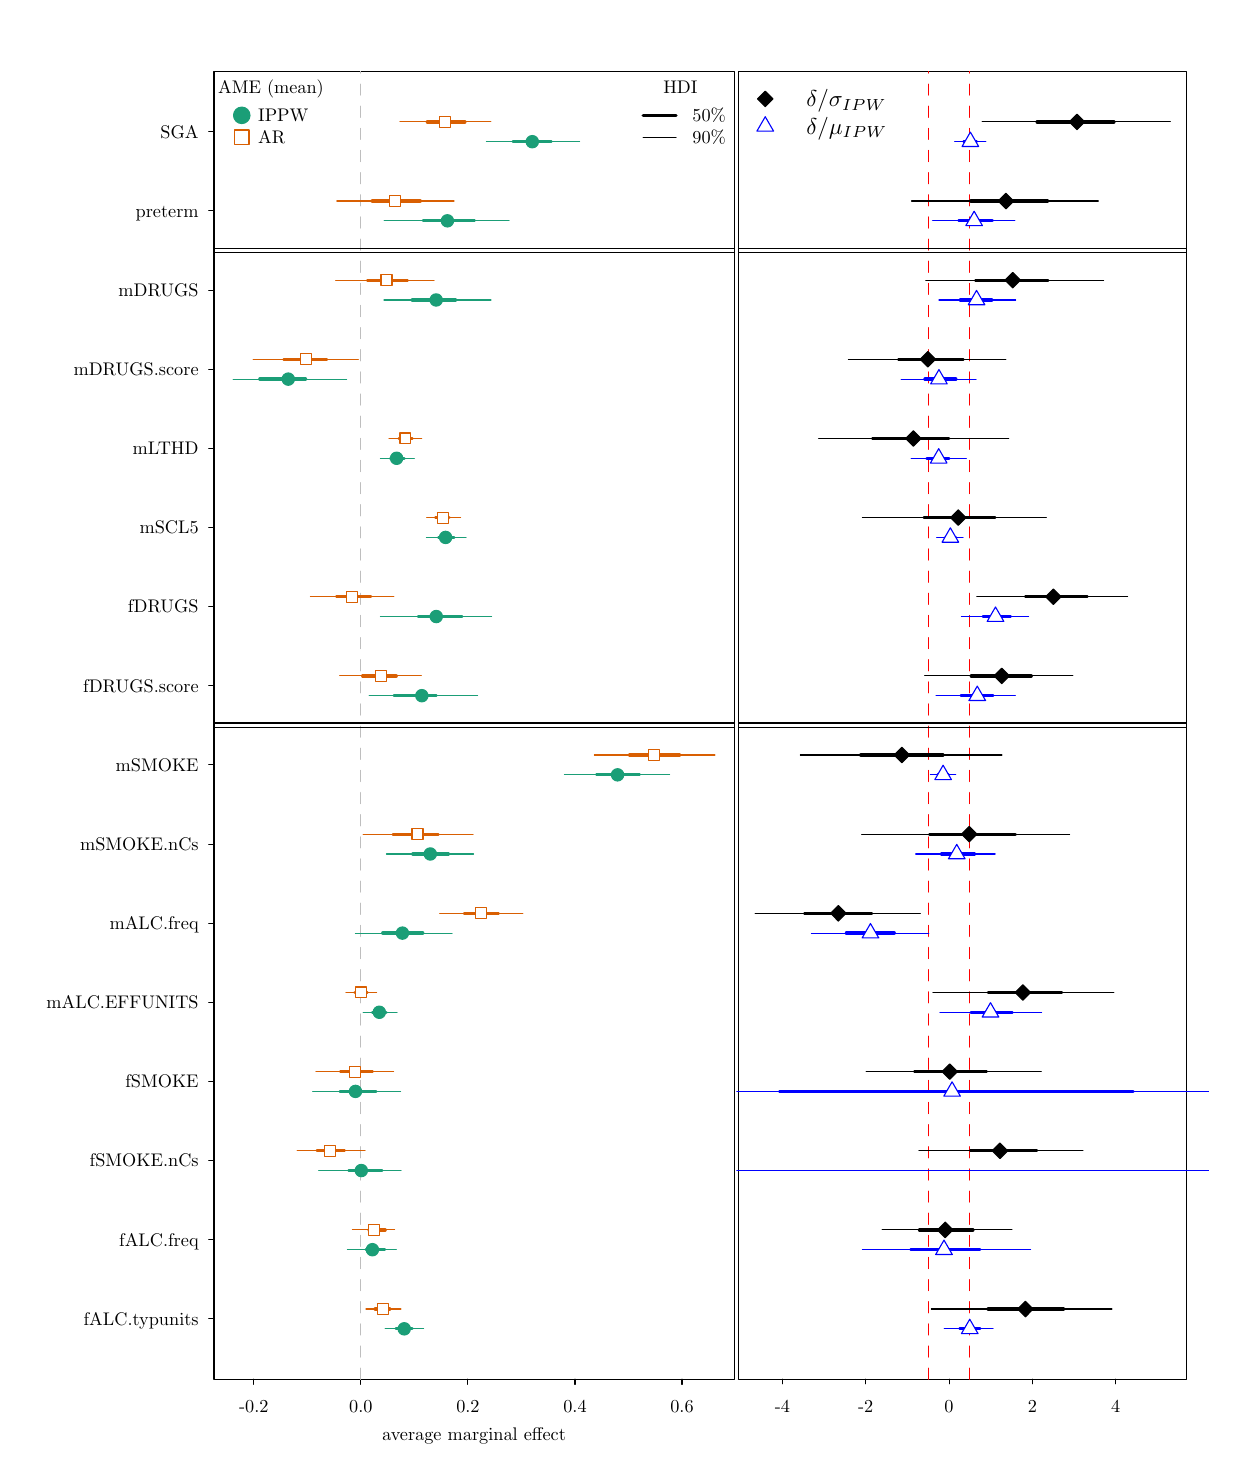
\begin{tikzpicture}[x=1pt,y=1pt]
\definecolor{fillColor}{RGB}{255,255,255}
\path[use as bounding box,fill=fillColor,fill opacity=0.00] (0,0) rectangle (426.79,512.15);
\begin{scope}
\path[clip] (  0.00,  0.00) rectangle (426.79,512.15);
\definecolor{drawColor}{RGB}{0,0,0}

\path[draw=drawColor,line width= 0.4pt,line join=round,line cap=round] ( 81.73, 23.76) -- (236.45, 23.76);

\path[draw=drawColor,line width= 0.4pt,line join=round,line cap=round] ( 81.73, 23.76) -- ( 81.73, 21.88);

\path[draw=drawColor,line width= 0.4pt,line join=round,line cap=round] (120.41, 23.76) -- (120.41, 21.88);

\path[draw=drawColor,line width= 0.4pt,line join=round,line cap=round] (159.09, 23.76) -- (159.09, 21.88);

\path[draw=drawColor,line width= 0.4pt,line join=round,line cap=round] (197.77, 23.76) -- (197.77, 21.88);

\path[draw=drawColor,line width= 0.4pt,line join=round,line cap=round] (236.45, 23.76) -- (236.45, 21.88);

\node[text=drawColor,anchor=base,inner sep=0pt, outer sep=0pt, scale=  0.66] at ( 81.73, 11.88) {-0.2};

\node[text=drawColor,anchor=base,inner sep=0pt, outer sep=0pt, scale=  0.66] at (120.41, 11.88) {0.0};

\node[text=drawColor,anchor=base,inner sep=0pt, outer sep=0pt, scale=  0.66] at (159.09, 11.88) {0.2};

\node[text=drawColor,anchor=base,inner sep=0pt, outer sep=0pt, scale=  0.66] at (197.77, 11.88) {0.4};

\node[text=drawColor,anchor=base,inner sep=0pt, outer sep=0pt, scale=  0.66] at (236.45, 11.88) {0.6};

\path[draw=drawColor,line width= 0.4pt,line join=round,line cap=round] ( 67.32, 23.76) --
	(255.28, 23.76) --
	(255.28,496.31) --
	( 67.32,496.31) --
	( 67.32, 23.76);
\end{scope}
\begin{scope}
\path[clip] (  0.00,  0.00) rectangle (256.07,512.15);
\definecolor{drawColor}{RGB}{0,0,0}

\node[text=drawColor,anchor=base,inner sep=0pt, outer sep=0pt, scale=  0.66] at (161.30,  1.58) {average marginal effect};
\end{scope}
\begin{scope}
\path[clip] ( 67.32, 23.76) rectangle (255.28,496.31);
\definecolor{drawColor}{RGB}{190,190,190}

\path[draw=drawColor,line width= 0.4pt,dash pattern=on 4pt off 4pt ,line join=round,line cap=round] (120.41, 23.76) -- (120.41,496.31);
\definecolor{drawColor}{RGB}{27,158,119}

\path[draw=drawColor,line width= 1.2pt,line join=round,line cap=round] (175.33,470.94) -- (189.22,470.94);

\path[draw=drawColor,line width= 1.2pt,line join=round,line cap=round] (142.87,442.35) -- (161.46,442.35);

\path[draw=drawColor,line width= 1.2pt,line join=round,line cap=round] (138.95,413.75) -- (154.58,413.75);

\path[draw=drawColor,line width= 1.2pt,line join=round,line cap=round] ( 83.89,385.15) -- (100.40,385.15);

\path[draw=drawColor,line width= 1.2pt,line join=round,line cap=round] (131.05,356.55) -- (136.06,356.55);

\path[draw=drawColor,line width= 1.2pt,line join=round,line cap=round] (148.43,327.95) -- (154.09,327.95);

\path[draw=drawColor,line width= 1.2pt,line join=round,line cap=round] (141.09,299.36) -- (156.98,299.36);

\path[draw=drawColor,line width= 1.2pt,line join=round,line cap=round] (132.35,270.76) -- (147.68,270.76);

\path[draw=drawColor,line width= 1.2pt,line join=round,line cap=round] (205.51,242.16) -- (221.12,242.16);

\path[draw=drawColor,line width= 1.2pt,line join=round,line cap=round] (139.19,213.56) -- (152.00,213.56);

\path[draw=drawColor,line width= 1.2pt,line join=round,line cap=round] (128.30,184.97) -- (142.75,184.97);

\path[draw=drawColor,line width= 1.2pt,line join=round,line cap=round] (124.54,156.37) -- (129.55,156.37);

\path[draw=drawColor,line width= 1.2pt,line join=round,line cap=round] (112.85,127.77) -- (125.88,127.77);

\path[draw=drawColor,line width= 1.2pt,line join=round,line cap=round] (116.00, 99.17) -- (128.07, 99.17);

\path[draw=drawColor,line width= 1.2pt,line join=round,line cap=round] (122.24, 70.57) -- (129.02, 70.57);

\path[draw=drawColor,line width= 1.2pt,line join=round,line cap=round] (133.09, 41.98) -- (138.95, 41.98);

\path[draw=drawColor,line width= 0.4pt,line join=round,line cap=round] (165.78,470.94) -- (199.46,470.94);

\path[draw=drawColor,line width= 0.4pt,line join=round,line cap=round] (128.81,442.35) -- (173.96,442.35);

\path[draw=drawColor,line width= 0.4pt,line join=round,line cap=round] (128.76,413.75) -- (167.41,413.75);

\path[draw=drawColor,line width= 0.4pt,line join=round,line cap=round] ( 74.28,385.15) -- (115.23,385.15);

\path[draw=drawColor,line width= 0.4pt,line join=round,line cap=round] (127.47,356.55) -- (139.76,356.55);

\path[draw=drawColor,line width= 0.4pt,line join=round,line cap=round] (144.12,327.95) -- (158.43,327.95);

\path[draw=drawColor,line width= 0.4pt,line join=round,line cap=round] (127.46,299.36) -- (167.62,299.36);

\path[draw=drawColor,line width= 0.4pt,line join=round,line cap=round] (123.42,270.76) -- (162.54,270.76);

\path[draw=drawColor,line width= 0.4pt,line join=round,line cap=round] (193.96,242.16) -- (231.99,242.16);

\path[draw=drawColor,line width= 0.4pt,line join=round,line cap=round] (129.64,213.56) -- (161.10,213.56);

\path[draw=drawColor,line width= 0.4pt,line join=round,line cap=round] (118.46,184.97) -- (153.33,184.97);

\path[draw=drawColor,line width= 0.4pt,line join=round,line cap=round] (121.20,156.37) -- (133.47,156.37);

\path[draw=drawColor,line width= 0.4pt,line join=round,line cap=round] (102.98,127.77) -- (134.74,127.77);

\path[draw=drawColor,line width= 0.4pt,line join=round,line cap=round] (105.17, 99.17) -- (134.93, 99.17);

\path[draw=drawColor,line width= 0.4pt,line join=round,line cap=round] (115.51, 70.57) -- (133.20, 70.57);

\path[draw=drawColor,line width= 0.4pt,line join=round,line cap=round] (129.17, 41.98) -- (143.08, 41.98);
\definecolor{fillColor}{RGB}{27,158,119}

\path[draw=drawColor,line width= 0.4pt,line join=round,line cap=round,fill=fillColor] (182.34,470.94) circle (  2.23);

\path[draw=drawColor,line width= 0.4pt,line join=round,line cap=round,fill=fillColor] (151.67,442.35) circle (  2.23);

\path[draw=drawColor,line width= 0.4pt,line join=round,line cap=round,fill=fillColor] (147.61,413.75) circle (  2.23);

\path[draw=drawColor,line width= 0.4pt,line join=round,line cap=round,fill=fillColor] ( 94.16,385.15) circle (  2.23);

\path[draw=drawColor,line width= 0.4pt,line join=round,line cap=round,fill=fillColor] (133.31,356.55) circle (  2.23);

\path[draw=drawColor,line width= 0.4pt,line join=round,line cap=round,fill=fillColor] (151.01,327.95) circle (  2.23);

\path[draw=drawColor,line width= 0.4pt,line join=round,line cap=round,fill=fillColor] (147.64,299.36) circle (  2.23);

\path[draw=drawColor,line width= 0.4pt,line join=round,line cap=round,fill=fillColor] (142.43,270.76) circle (  2.23);

\path[draw=drawColor,line width= 0.4pt,line join=round,line cap=round,fill=fillColor] (213.15,242.16) circle (  2.23);

\path[draw=drawColor,line width= 0.4pt,line join=round,line cap=round,fill=fillColor] (145.48,213.56) circle (  2.23);

\path[draw=drawColor,line width= 0.4pt,line join=round,line cap=round,fill=fillColor] (135.42,184.97) circle (  2.23);

\path[draw=drawColor,line width= 0.4pt,line join=round,line cap=round,fill=fillColor] (127.07,156.37) circle (  2.23);

\path[draw=drawColor,line width= 0.4pt,line join=round,line cap=round,fill=fillColor] (118.44,127.77) circle (  2.23);

\path[draw=drawColor,line width= 0.4pt,line join=round,line cap=round,fill=fillColor] (120.56, 99.17) circle (  2.23);

\path[draw=drawColor,line width= 0.4pt,line join=round,line cap=round,fill=fillColor] (124.57, 70.57) circle (  2.23);

\path[draw=drawColor,line width= 0.4pt,line join=round,line cap=round,fill=fillColor] (136.07, 41.98) circle (  2.23);
\definecolor{drawColor}{RGB}{217,95,2}

\path[draw=drawColor,line width= 1.2pt,line join=round,line cap=round] (144.42,478.09) -- (157.97,478.09);

\path[draw=drawColor,line width= 1.2pt,line join=round,line cap=round] (124.49,449.50) -- (141.84,449.50);

\path[draw=drawColor,line width= 1.2pt,line join=round,line cap=round] (122.73,420.90) -- (137.26,420.90);

\path[draw=drawColor,line width= 1.2pt,line join=round,line cap=round] ( 92.52,392.30) -- (108.08,392.30);

\path[draw=drawColor,line width= 1.2pt,line join=round,line cap=round] (134.16,363.70) -- (138.97,363.70);

\path[draw=drawColor,line width= 1.2pt,line join=round,line cap=round] (147.35,335.10) -- (152.31,335.10);

\path[draw=drawColor,line width= 1.2pt,line join=round,line cap=round] (111.54,306.51) -- (124.03,306.51);

\path[draw=drawColor,line width= 1.2pt,line join=round,line cap=round] (121.04,277.91) -- (133.17,277.91);

\path[draw=drawColor,line width= 1.2pt,line join=round,line cap=round] (217.51,249.31) -- (235.54,249.31);

\path[draw=drawColor,line width= 1.2pt,line join=round,line cap=round] (131.96,220.71) -- (148.38,220.71);

\path[draw=drawColor,line width= 1.2pt,line join=round,line cap=round] (157.74,192.12) -- (170.18,192.12);

\path[draw=drawColor,line width= 1.2pt,line join=round,line cap=round] (118.21,163.52) -- (122.75,163.52);

\path[draw=drawColor,line width= 1.2pt,line join=round,line cap=round] (112.98,134.92) -- (124.62,134.92);

\path[draw=drawColor,line width= 1.2pt,line join=round,line cap=round] (104.50,106.32) -- (114.48,106.32);

\path[draw=drawColor,line width= 1.2pt,line join=round,line cap=round] (123.36, 77.72) -- (129.17, 77.72);

\path[draw=drawColor,line width= 1.2pt,line join=round,line cap=round] (125.57, 49.13) -- (130.80, 49.13);

\path[draw=drawColor,line width= 0.4pt,line join=round,line cap=round] (134.51,478.09) -- (167.37,478.09);

\path[draw=drawColor,line width= 0.4pt,line join=round,line cap=round] (111.72,449.50) -- (154.06,449.50);

\path[draw=drawColor,line width= 0.4pt,line join=round,line cap=round] (111.26,420.90) -- (146.87,420.90);

\path[draw=drawColor,line width= 0.4pt,line join=round,line cap=round] ( 81.47,392.30) -- (119.49,392.30);

\path[draw=drawColor,line width= 0.4pt,line join=round,line cap=round] (130.57,363.70) -- (142.38,363.70);

\path[draw=drawColor,line width= 0.4pt,line join=round,line cap=round] (144.16,335.10) -- (156.44,335.10);

\path[draw=drawColor,line width= 0.4pt,line join=round,line cap=round] (102.16,306.51) -- (132.30,306.51);

\path[draw=drawColor,line width= 0.4pt,line join=round,line cap=round] (112.72,277.91) -- (142.22,277.91);

\path[draw=drawColor,line width= 0.4pt,line join=round,line cap=round] (204.77,249.31) -- (248.32,249.31);

\path[draw=drawColor,line width= 0.4pt,line join=round,line cap=round] (121.26,220.71) -- (160.95,220.71);

\path[draw=drawColor,line width= 0.4pt,line join=round,line cap=round] (148.87,192.12) -- (178.91,192.12);

\path[draw=drawColor,line width= 0.4pt,line join=round,line cap=round] (114.98,163.52) -- (126.07,163.52);

\path[draw=drawColor,line width= 0.4pt,line join=round,line cap=round] (104.12,134.92) -- (132.21,134.92);

\path[draw=drawColor,line width= 0.4pt,line join=round,line cap=round] ( 97.41,106.32) -- (121.89,106.32);

\path[draw=drawColor,line width= 0.4pt,line join=round,line cap=round] (117.36, 77.72) -- (132.56, 77.72);

\path[draw=drawColor,line width= 0.4pt,line join=round,line cap=round] (122.25, 49.13) -- (134.87, 49.13);
\definecolor{fillColor}{RGB}{255,255,255}

\path[draw=drawColor,line width= 0.4pt,line join=round,line cap=round,fill=fillColor] (148.70,476.12) rectangle (152.65,480.07);

\path[draw=drawColor,line width= 0.4pt,line join=round,line cap=round,fill=fillColor] (130.88,447.52) rectangle (134.83,451.47);

\path[draw=drawColor,line width= 0.4pt,line join=round,line cap=round,fill=fillColor] (127.69,418.92) rectangle (131.64,422.87);

\path[draw=drawColor,line width= 0.4pt,line join=round,line cap=round,fill=fillColor] ( 98.54,390.33) rectangle (102.49,394.27);

\path[draw=drawColor,line width= 0.4pt,line join=round,line cap=round,fill=fillColor] (134.54,361.73) rectangle (138.49,365.68);

\path[draw=drawColor,line width= 0.4pt,line join=round,line cap=round,fill=fillColor] (148.07,333.13) rectangle (152.02,337.08);

\path[draw=drawColor,line width= 0.4pt,line join=round,line cap=round,fill=fillColor] (115.31,304.53) rectangle (119.26,308.48);

\path[draw=drawColor,line width= 0.4pt,line join=round,line cap=round,fill=fillColor] (125.55,275.93) rectangle (129.50,279.88);

\path[draw=drawColor,line width= 0.4pt,line join=round,line cap=round,fill=fillColor] (224.38,247.34) rectangle (228.33,251.28);

\path[draw=drawColor,line width= 0.4pt,line join=round,line cap=round,fill=fillColor] (138.88,218.74) rectangle (142.83,222.69);

\path[draw=drawColor,line width= 0.4pt,line join=round,line cap=round,fill=fillColor] (161.75,190.14) rectangle (165.70,194.09);

\path[draw=drawColor,line width= 0.4pt,line join=round,line cap=round,fill=fillColor] (118.47,161.54) rectangle (122.42,165.49);

\path[draw=drawColor,line width= 0.4pt,line join=round,line cap=round,fill=fillColor] (116.32,132.95) rectangle (120.27,136.89);

\path[draw=drawColor,line width= 0.4pt,line join=round,line cap=round,fill=fillColor] (107.23,104.35) rectangle (111.18,108.30);

\path[draw=drawColor,line width= 0.4pt,line join=round,line cap=round,fill=fillColor] (123.10, 75.75) rectangle (127.05, 79.70);

\path[draw=drawColor,line width= 0.4pt,line join=round,line cap=round,fill=fillColor] (126.32, 47.15) rectangle (130.27, 51.10);
\end{scope}
\begin{scope}
\path[clip] (  0.00,  0.00) rectangle (426.79,512.15);
\definecolor{drawColor}{RGB}{0,0,0}

\path[draw=drawColor,line width= 0.4pt,line join=round,line cap=round] ( 67.32, 45.55) -- ( 67.32,474.52);

\path[draw=drawColor,line width= 0.4pt,line join=round,line cap=round] ( 67.32, 45.55) -- ( 65.44, 45.55);

\path[draw=drawColor,line width= 0.4pt,line join=round,line cap=round] ( 67.32, 74.15) -- ( 65.44, 74.15);

\path[draw=drawColor,line width= 0.4pt,line join=round,line cap=round] ( 67.32,102.75) -- ( 65.44,102.75);

\path[draw=drawColor,line width= 0.4pt,line join=round,line cap=round] ( 67.32,131.34) -- ( 65.44,131.34);

\path[draw=drawColor,line width= 0.4pt,line join=round,line cap=round] ( 67.32,159.94) -- ( 65.44,159.94);

\path[draw=drawColor,line width= 0.4pt,line join=round,line cap=round] ( 67.32,188.54) -- ( 65.44,188.54);

\path[draw=drawColor,line width= 0.4pt,line join=round,line cap=round] ( 67.32,217.14) -- ( 65.44,217.14);

\path[draw=drawColor,line width= 0.4pt,line join=round,line cap=round] ( 67.32,245.74) -- ( 65.44,245.74);

\path[draw=drawColor,line width= 0.4pt,line join=round,line cap=round] ( 67.32,274.33) -- ( 65.44,274.33);

\path[draw=drawColor,line width= 0.4pt,line join=round,line cap=round] ( 67.32,302.93) -- ( 65.44,302.93);

\path[draw=drawColor,line width= 0.4pt,line join=round,line cap=round] ( 67.32,331.53) -- ( 65.44,331.53);

\path[draw=drawColor,line width= 0.4pt,line join=round,line cap=round] ( 67.32,360.13) -- ( 65.44,360.13);

\path[draw=drawColor,line width= 0.4pt,line join=round,line cap=round] ( 67.32,388.72) -- ( 65.44,388.72);

\path[draw=drawColor,line width= 0.4pt,line join=round,line cap=round] ( 67.32,417.32) -- ( 65.44,417.32);

\path[draw=drawColor,line width= 0.4pt,line join=round,line cap=round] ( 67.32,445.92) -- ( 65.44,445.92);

\path[draw=drawColor,line width= 0.4pt,line join=round,line cap=round] ( 67.32,474.52) -- ( 65.44,474.52);

\node[text=drawColor,anchor=base east,inner sep=0pt, outer sep=0pt, scale=  0.66] at ( 61.78, 43.28) {fALC.typunits};

\node[text=drawColor,anchor=base east,inner sep=0pt, outer sep=0pt, scale=  0.66] at ( 61.78, 71.88) {fALC.freq};

\node[text=drawColor,anchor=base east,inner sep=0pt, outer sep=0pt, scale=  0.66] at ( 61.78,100.47) {fSMOKE.nCs};

\node[text=drawColor,anchor=base east,inner sep=0pt, outer sep=0pt, scale=  0.66] at ( 61.78,129.07) {fSMOKE};

\node[text=drawColor,anchor=base east,inner sep=0pt, outer sep=0pt, scale=  0.66] at ( 61.78,157.67) {mALC.EFFUNITS};

\node[text=drawColor,anchor=base east,inner sep=0pt, outer sep=0pt, scale=  0.66] at ( 61.78,186.27) {mALC.freq};

\node[text=drawColor,anchor=base east,inner sep=0pt, outer sep=0pt, scale=  0.66] at ( 61.78,214.87) {mSMOKE.nCs};

\node[text=drawColor,anchor=base east,inner sep=0pt, outer sep=0pt, scale=  0.66] at ( 61.78,243.46) {mSMOKE};

\node[text=drawColor,anchor=base east,inner sep=0pt, outer sep=0pt, scale=  0.66] at ( 61.78,272.06) {fDRUGS.score};

\node[text=drawColor,anchor=base east,inner sep=0pt, outer sep=0pt, scale=  0.66] at ( 61.78,300.66) {fDRUGS};

\node[text=drawColor,anchor=base east,inner sep=0pt, outer sep=0pt, scale=  0.66] at ( 61.78,329.26) {mSCL5};

\node[text=drawColor,anchor=base east,inner sep=0pt, outer sep=0pt, scale=  0.66] at ( 61.78,357.85) {mLTHD};

\node[text=drawColor,anchor=base east,inner sep=0pt, outer sep=0pt, scale=  0.66] at ( 61.78,386.45) {mDRUGS.score};

\node[text=drawColor,anchor=base east,inner sep=0pt, outer sep=0pt, scale=  0.66] at ( 61.78,415.05) {mDRUGS};

\node[text=drawColor,anchor=base east,inner sep=0pt, outer sep=0pt, scale=  0.66] at ( 61.78,443.65) {preterm};

\node[text=drawColor,anchor=base east,inner sep=0pt, outer sep=0pt, scale=  0.66] at ( 61.78,472.25) {SGA};
\end{scope}
\begin{scope}
\path[clip] ( 67.32, 23.76) rectangle (255.28,496.31);
\definecolor{drawColor}{RGB}{27,158,119}
\definecolor{fillColor}{RGB}{27,158,119}

\path[draw=drawColor,line width= 0.4pt,line join=round,line cap=round,fill=fillColor] ( 77.36,480.47) circle (  2.97);
\definecolor{drawColor}{RGB}{217,95,2}
\definecolor{fillColor}{RGB}{255,255,255}

\path[draw=drawColor,line width= 0.4pt,line join=round,line cap=round,fill=fillColor] ( 74.72,469.92) rectangle ( 79.99,475.18);
\definecolor{drawColor}{RGB}{0,0,0}

\node[text=drawColor,anchor=base,inner sep=0pt, outer sep=0pt, scale=  0.66] at ( 87.91,488.39) {AME (mean)};

\node[text=drawColor,anchor=base west,inner sep=0pt, outer sep=0pt, scale=  0.66] at ( 83.30,478.20) {IPPW};

\node[text=drawColor,anchor=base west,inner sep=0pt, outer sep=0pt, scale=  0.66] at ( 83.30,470.28) {AR};

\path[draw=drawColor,line width= 1.2pt,line join=round,line cap=round] (222.40,480.47) -- (234.28,480.47);

\path[draw=drawColor,line width= 0.4pt,line join=round,line cap=round] (222.40,472.55) -- (234.28,472.55);

\node[text=drawColor,anchor=base,inner sep=0pt, outer sep=0pt, scale=  0.66] at (235.87,488.39) {HDI};

\node[text=drawColor,anchor=base west,inner sep=0pt, outer sep=0pt, scale=  0.66] at (240.22,478.20) {50\%};

\node[text=drawColor,anchor=base west,inner sep=0pt, outer sep=0pt, scale=  0.66] at (240.22,470.28) {90\%};

\path[draw=drawColor,line width= 0.4pt,line join=round,line cap=round] ( 67.32,430.76) -- (255.28,430.76);

\path[draw=drawColor,line width= 0.4pt,line join=round,line cap=round] ( 67.32,432.48) -- (255.28,432.48);

\path[draw=drawColor,line width= 0.4pt,line join=round,line cap=round] ( 67.32,259.18) -- (255.28,259.18);

\path[draw=drawColor,line width= 0.4pt,line join=round,line cap=round] ( 67.32,260.89) -- (255.28,260.89);
\end{scope}
\begin{scope}
\path[clip] (  0.00,  0.00) rectangle (426.79,512.15);
\definecolor{drawColor}{RGB}{0,0,0}

\path[draw=drawColor,line width= 0.4pt,line join=round,line cap=round] (272.72, 23.76) -- (393.15, 23.76);

\path[draw=drawColor,line width= 0.4pt,line join=round,line cap=round] (272.72, 23.76) -- (272.72, 22.14);

\path[draw=drawColor,line width= 0.4pt,line join=round,line cap=round] (302.83, 23.76) -- (302.83, 22.14);

\path[draw=drawColor,line width= 0.4pt,line join=round,line cap=round] (332.94, 23.76) -- (332.94, 22.14);

\path[draw=drawColor,line width= 0.4pt,line join=round,line cap=round] (363.05, 23.76) -- (363.05, 22.14);

\path[draw=drawColor,line width= 0.4pt,line join=round,line cap=round] (393.15, 23.76) -- (393.15, 22.14);

\node[text=drawColor,anchor=base,inner sep=0pt, outer sep=0pt, scale=  0.66] at (272.72, 11.88) {-4};

\node[text=drawColor,anchor=base,inner sep=0pt, outer sep=0pt, scale=  0.66] at (302.83, 11.88) {-2};

\node[text=drawColor,anchor=base,inner sep=0pt, outer sep=0pt, scale=  0.66] at (332.94, 11.88) {0};

\node[text=drawColor,anchor=base,inner sep=0pt, outer sep=0pt, scale=  0.66] at (363.05, 11.88) {2};

\node[text=drawColor,anchor=base,inner sep=0pt, outer sep=0pt, scale=  0.66] at (393.15, 11.88) {4};

\path[draw=drawColor,line width= 0.4pt,line join=round,line cap=round] (256.87, 23.76) --
	(418.87, 23.76) --
	(418.87,496.31) --
	(256.87,496.31) --
	(256.87, 23.76);
\end{scope}
\begin{scope}
\path[clip] (256.87, 23.76) rectangle (418.87,496.31);
\definecolor{drawColor}{RGB}{255,0,0}

\path[draw=drawColor,line width= 0.4pt,dash pattern=on 4pt off 4pt ,line join=round,line cap=round] (325.41, 23.76) -- (325.41,496.31);

\path[draw=drawColor,line width= 0.4pt,dash pattern=on 4pt off 4pt ,line join=round,line cap=round] (340.47, 23.76) -- (340.47,496.31);
\end{scope}
\begin{scope}
\path[clip] (256.07,  0.00) rectangle (426.79,512.15);
\definecolor{drawColor}{RGB}{0,0,0}

\path[draw=drawColor,line width= 0.4pt,line join=round,line cap=round] (344.92,478.09) -- (412.87,478.09);

\path[draw=drawColor,line width= 0.4pt,line join=round,line cap=round] (319.39,449.50) -- (386.85,449.50);

\path[draw=drawColor,line width= 0.4pt,line join=round,line cap=round] (324.53,420.90) -- (388.76,420.90);

\path[draw=drawColor,line width= 0.4pt,line join=round,line cap=round] (296.54,392.30) -- (353.45,392.30);

\path[draw=drawColor,line width= 0.4pt,line join=round,line cap=round] (285.78,363.70) -- (354.49,363.70);

\path[draw=drawColor,line width= 0.4pt,line join=round,line cap=round] (301.63,335.10) -- (368.09,335.10);

\path[draw=drawColor,line width= 0.4pt,line join=round,line cap=round] (342.96,306.51) -- (397.47,306.51);

\path[draw=drawColor,line width= 0.4pt,line join=round,line cap=round] (324.16,277.91) -- (377.63,277.91);

\path[draw=drawColor,line width= 0.4pt,line join=round,line cap=round] (279.20,249.31) -- (352.04,249.31);

\path[draw=drawColor,line width= 0.4pt,line join=round,line cap=round] (301.38,220.71) -- (376.52,220.71);

\path[draw=drawColor,line width= 0.4pt,line join=round,line cap=round] (262.87,192.12) -- (322.58,192.12);

\path[draw=drawColor,line width= 0.4pt,line join=round,line cap=round] (327.08,163.52) -- (392.47,163.52);

\path[draw=drawColor,line width= 0.4pt,line join=round,line cap=round] (303.00,134.92) -- (366.24,134.92);

\path[draw=drawColor,line width= 0.4pt,line join=round,line cap=round] (322.05,106.32) -- (381.32,106.32);

\path[draw=drawColor,line width= 0.4pt,line join=round,line cap=round] (308.74, 77.72) -- (355.67, 77.72);

\path[draw=drawColor,line width= 0.4pt,line join=round,line cap=round] (326.55, 49.13) -- (391.78, 49.13);

\path[draw=drawColor,line width= 1.2pt,line join=round,line cap=round] (364.77,478.09) -- (392.50,478.09);

\path[draw=drawColor,line width= 1.2pt,line join=round,line cap=round] (340.80,449.50) -- (368.51,449.50);

\path[draw=drawColor,line width= 1.2pt,line join=round,line cap=round] (342.45,420.90) -- (368.72,420.90);

\path[draw=drawColor,line width= 1.2pt,line join=round,line cap=round] (314.62,392.30) -- (338.08,392.30);

\path[draw=drawColor,line width= 1.2pt,line join=round,line cap=round] (305.25,363.70) -- (332.89,363.70);

\path[draw=drawColor,line width= 1.2pt,line join=round,line cap=round] (323.86,335.10) -- (349.56,335.10);

\path[draw=drawColor,line width= 1.2pt,line join=round,line cap=round] (360.50,306.51) -- (382.92,306.51);

\path[draw=drawColor,line width= 1.2pt,line join=round,line cap=round] (340.98,277.91) -- (362.62,277.91);

\path[draw=drawColor,line width= 1.2pt,line join=round,line cap=round] (301.02,249.31) -- (330.72,249.31);

\path[draw=drawColor,line width= 1.2pt,line join=round,line cap=round] (325.88,220.71) -- (356.93,220.71);

\path[draw=drawColor,line width= 1.2pt,line join=round,line cap=round] (280.68,192.12) -- (305.02,192.12);

\path[draw=drawColor,line width= 1.2pt,line join=round,line cap=round] (347.04,163.52) -- (373.65,163.52);

\path[draw=drawColor,line width= 1.2pt,line join=round,line cap=round] (320.45,134.92) -- (346.49,134.92);

\path[draw=drawColor,line width= 1.2pt,line join=round,line cap=round] (340.67,106.32) -- (364.64,106.32);

\path[draw=drawColor,line width= 1.2pt,line join=round,line cap=round] (322.25, 77.72) -- (341.55, 77.72);

\path[draw=drawColor,line width= 1.2pt,line join=round,line cap=round] (347.07, 49.13) -- (374.29, 49.13);
\definecolor{drawColor}{RGB}{0,0,255}

\path[draw=drawColor,line width= 0.4pt,line join=round,line cap=round] (334.93,470.94) -- (346.26,470.94);

\path[draw=drawColor,line width= 0.4pt,line join=round,line cap=round] (326.97,442.35) -- (356.70,442.35);

\path[draw=drawColor,line width= 0.4pt,line join=round,line cap=round] (329.31,413.75) -- (357.01,413.75);

\path[draw=drawColor,line width= 0.4pt,line join=round,line cap=round] (315.63,385.15) -- (342.69,385.15);

\path[draw=drawColor,line width= 0.4pt,line join=round,line cap=round] (319.23,356.55) -- (339.20,356.55);

\path[draw=drawColor,line width= 0.4pt,line join=round,line cap=round] (328.42,327.95) -- (338.01,327.95);

\path[draw=drawColor,line width= 0.4pt,line join=round,line cap=round] (337.40,299.36) -- (361.67,299.36);

\path[draw=drawColor,line width= 0.4pt,line join=round,line cap=round] (328.23,270.76) -- (356.87,270.76);

\path[draw=drawColor,line width= 0.4pt,line join=round,line cap=round] (326.19,242.16) -- (335.34,242.16);

\path[draw=drawColor,line width= 0.4pt,line join=round,line cap=round] (320.89,213.56) -- (349.58,213.56);

\path[draw=drawColor,line width= 0.4pt,line join=round,line cap=round] (283.21,184.97) -- (325.59,184.97);

\path[draw=drawColor,line width= 0.4pt,line join=round,line cap=round] (329.65,156.37) -- (366.36,156.37);

\path[draw=drawColor,line width= 0.4pt,line join=round,line cap=round] (185.92,127.77) -- (426.79,127.77);

\path[draw=drawColor,line width= 0.4pt,line join=round,line cap=round] (  0.00, 99.17) -- (426.79, 99.17);

\path[draw=drawColor,line width= 0.4pt,line join=round,line cap=round] (301.59, 70.57) -- (362.39, 70.57);

\path[draw=drawColor,line width= 0.4pt,line join=round,line cap=round] (331.21, 41.98) -- (348.87, 41.98);

\path[draw=drawColor,line width= 1.2pt,line join=round,line cap=round] (338.24,470.94) -- (342.86,470.94);

\path[draw=drawColor,line width= 1.2pt,line join=round,line cap=round] (336.40,442.35) -- (348.62,442.35);

\path[draw=drawColor,line width= 1.2pt,line join=round,line cap=round] (337.04,413.75) -- (348.37,413.75);

\path[draw=drawColor,line width= 1.2pt,line join=round,line cap=round] (324.23,385.15) -- (335.38,385.15);

\path[draw=drawColor,line width= 1.2pt,line join=round,line cap=round] (324.89,356.55) -- (332.92,356.55);

\path[draw=drawColor,line width= 1.2pt,line join=round,line cap=round] (331.63,327.95) -- (335.34,327.95);

\path[draw=drawColor,line width= 1.2pt,line join=round,line cap=round] (345.21,299.36) -- (355.19,299.36);

\path[draw=drawColor,line width= 1.2pt,line join=round,line cap=round] (337.25,270.76) -- (348.83,270.76);

\path[draw=drawColor,line width= 1.2pt,line join=round,line cap=round] (328.93,242.16) -- (332.66,242.16);

\path[draw=drawColor,line width= 1.2pt,line join=round,line cap=round] (330.24,213.56) -- (342.10,213.56);

\path[draw=drawColor,line width= 1.2pt,line join=round,line cap=round] (295.85,184.97) -- (313.13,184.97);

\path[draw=drawColor,line width= 1.2pt,line join=round,line cap=round] (340.85,156.37) -- (355.79,156.37);

\path[draw=drawColor,line width= 1.2pt,line join=round,line cap=round] (271.62,127.77) -- (399.48,127.77);

\path[draw=drawColor,line width= 1.2pt,line join=round,line cap=round] (319.10, 70.57) -- (344.10, 70.57);

\path[draw=drawColor,line width= 1.2pt,line join=round,line cap=round] (336.77, 41.98) -- (344.13, 41.98);
\definecolor{drawColor}{RGB}{0,0,0}
\definecolor{fillColor}{RGB}{0,0,0}

\path[draw=drawColor,line width= 0.4pt,line join=round,line cap=round,fill=fillColor] (379.14,475.30) --
	(381.93,478.09) --
	(379.14,480.88) --
	(376.35,478.09) --
	cycle;

\path[draw=drawColor,line width= 0.4pt,line join=round,line cap=round,fill=fillColor] (353.50,446.70) --
	(356.29,449.50) --
	(353.50,452.29) --
	(350.71,449.50) --
	cycle;

\path[draw=drawColor,line width= 0.4pt,line join=round,line cap=round,fill=fillColor] (355.97,418.11) --
	(358.76,420.90) --
	(355.97,423.69) --
	(353.18,420.90) --
	cycle;

\path[draw=drawColor,line width= 0.4pt,line join=round,line cap=round,fill=fillColor] (325.28,389.51) --
	(328.07,392.30) --
	(325.28,395.09) --
	(322.48,392.30) --
	cycle;

\path[draw=drawColor,line width= 0.4pt,line join=round,line cap=round,fill=fillColor] (320.08,360.91) --
	(322.87,363.70) --
	(320.08,366.49) --
	(317.29,363.70) --
	cycle;

\path[draw=drawColor,line width= 0.4pt,line join=round,line cap=round,fill=fillColor] (336.23,332.31) --
	(339.02,335.10) --
	(336.23,337.90) --
	(333.44,335.10) --
	cycle;

\path[draw=drawColor,line width= 0.4pt,line join=round,line cap=round,fill=fillColor] (370.63,303.71) --
	(373.43,306.51) --
	(370.63,309.30) --
	(367.84,306.51) --
	cycle;

\path[draw=drawColor,line width= 0.4pt,line join=round,line cap=round,fill=fillColor] (351.96,275.12) --
	(354.75,277.91) --
	(351.96,280.70) --
	(349.17,277.91) --
	cycle;

\path[draw=drawColor,line width= 0.4pt,line join=round,line cap=round,fill=fillColor] (315.87,246.52) --
	(318.66,249.31) --
	(315.87,252.10) --
	(313.08,249.31) --
	cycle;

\path[draw=drawColor,line width= 0.4pt,line join=round,line cap=round,fill=fillColor] (340.22,217.92) --
	(343.01,220.71) --
	(340.22,223.50) --
	(337.43,220.71) --
	cycle;

\path[draw=drawColor,line width= 0.4pt,line join=round,line cap=round,fill=fillColor] (292.93,189.32) --
	(295.72,192.12) --
	(292.93,194.91) --
	(290.14,192.12) --
	cycle;

\path[draw=drawColor,line width= 0.4pt,line join=round,line cap=round,fill=fillColor] (359.62,160.73) --
	(362.41,163.52) --
	(359.62,166.31) --
	(356.82,163.52) --
	cycle;

\path[draw=drawColor,line width= 0.4pt,line join=round,line cap=round,fill=fillColor] (333.16,132.13) --
	(335.95,134.92) --
	(333.16,137.71) --
	(330.37,134.92) --
	cycle;

\path[draw=drawColor,line width= 0.4pt,line join=round,line cap=round,fill=fillColor] (351.34,103.53) --
	(354.13,106.32) --
	(351.34,109.11) --
	(348.55,106.32) --
	cycle;

\path[draw=drawColor,line width= 0.4pt,line join=round,line cap=round,fill=fillColor] (331.53, 74.93) --
	(334.32, 77.72) --
	(331.53, 80.52) --
	(328.74, 77.72) --
	cycle;

\path[draw=drawColor,line width= 0.4pt,line join=round,line cap=round,fill=fillColor] (360.54, 46.33) --
	(363.33, 49.13) --
	(360.54, 51.92) --
	(357.75, 49.13) --
	cycle;
\definecolor{drawColor}{RGB}{0,0,255}
\definecolor{fillColor}{RGB}{255,255,255}

\path[draw=drawColor,line width= 0.4pt,line join=round,line cap=round,fill=fillColor] (340.64,474.41) --
	(343.64,469.21) --
	(337.64,469.21) --
	cycle;

\path[draw=drawColor,line width= 0.4pt,line join=round,line cap=round,fill=fillColor] (342.00,445.81) --
	(345.00,440.61) --
	(339.00,440.61) --
	cycle;

\path[draw=drawColor,line width= 0.4pt,line join=round,line cap=round,fill=fillColor] (342.87,417.21) --
	(345.87,412.02) --
	(339.87,412.02) --
	cycle;

\path[draw=drawColor,line width= 0.4pt,line join=round,line cap=round,fill=fillColor] (329.29,388.61) --
	(332.29,383.42) --
	(326.29,383.42) --
	cycle;

\path[draw=drawColor,line width= 0.4pt,line join=round,line cap=round,fill=fillColor] (329.20,360.02) --
	(332.20,354.82) --
	(326.20,354.82) --
	cycle;

\path[draw=drawColor,line width= 0.4pt,line join=round,line cap=round,fill=fillColor] (333.41,331.42) --
	(336.41,326.22) --
	(330.41,326.22) --
	cycle;

\path[draw=drawColor,line width= 0.4pt,line join=round,line cap=round,fill=fillColor] (349.72,302.82) --
	(352.72,297.62) --
	(346.72,297.62) --
	cycle;

\path[draw=drawColor,line width= 0.4pt,line join=round,line cap=round,fill=fillColor] (343.13,274.22) --
	(346.13,269.03) --
	(340.13,269.03) --
	cycle;

\path[draw=drawColor,line width= 0.4pt,line join=round,line cap=round,fill=fillColor] (330.79,245.63) --
	(333.79,240.43) --
	(327.79,240.43) --
	cycle;

\path[draw=drawColor,line width= 0.4pt,line join=round,line cap=round,fill=fillColor] (335.72,217.03) --
	(338.72,211.83) --
	(332.72,211.83) --
	cycle;

\path[draw=drawColor,line width= 0.4pt,line join=round,line cap=round,fill=fillColor] (304.54,188.43) --
	(307.54,183.23) --
	(301.54,183.23) --
	cycle;

\path[draw=drawColor,line width= 0.4pt,line join=round,line cap=round,fill=fillColor] (347.91,159.83) --
	(350.91,154.64) --
	(344.91,154.64) --
	cycle;

\path[draw=drawColor,line width= 0.4pt,line join=round,line cap=round,fill=fillColor] (334.03,131.23) --
	(337.03,126.04) --
	(331.03,126.04) --
	cycle;

\path[draw=drawColor,line width= 0.4pt,line join=round,line cap=round,fill=fillColor] (331.11, 74.04) --
	(334.11, 68.84) --
	(328.11, 68.84) --
	cycle;

\path[draw=drawColor,line width= 0.4pt,line join=round,line cap=round,fill=fillColor] (340.41, 45.44) --
	(343.41, 40.24) --
	(337.41, 40.24) --
	cycle;
\definecolor{drawColor}{RGB}{0,0,0}
\definecolor{fillColor}{RGB}{0,0,0}

\path[draw=drawColor,line width= 0.4pt,line join=round,line cap=round,fill=fillColor] (266.52,483.62) --
	(269.31,486.41) --
	(266.52,489.20) --
	(263.73,486.41) --
	cycle;
\definecolor{drawColor}{RGB}{0,0,255}
\definecolor{fillColor}{RGB}{255,255,255}

\path[draw=drawColor,line width= 0.4pt,line join=round,line cap=round,fill=fillColor] (266.52,479.97) --
	(269.52,474.78) --
	(263.52,474.78) --
	cycle;
\definecolor{drawColor}{RGB}{0,0,0}

\node[text=drawColor,anchor=base west,inner sep=0pt, outer sep=0pt, scale=  0.83] at (281.37,483.57) {$\delta/\sigma_{IPW}$};

\node[text=drawColor,anchor=base west,inner sep=0pt, outer sep=0pt, scale=  0.83] at (281.37,473.67) {$\delta/\mu_{IPW}$};
\end{scope}
\begin{scope}
\path[clip] (256.87, 23.76) rectangle (418.87,496.31);
\definecolor{drawColor}{RGB}{0,0,0}

\path[draw=drawColor,line width= 0.4pt,line join=round,line cap=round] (256.87,430.76) -- (418.87,430.76);

\path[draw=drawColor,line width= 0.4pt,line join=round,line cap=round] (256.87,432.48) -- (418.87,432.48);

\path[draw=drawColor,line width= 0.4pt,line join=round,line cap=round] (256.87,259.18) -- (418.87,259.18);

\path[draw=drawColor,line width= 0.4pt,line join=round,line cap=round] (256.87,260.89) -- (418.87,260.89);
\end{scope}
\end{tikzpicture}



\section{Discussion}
Bias due to self-selection into studies and selective dropout is a threat to the validity of exposure outcome estimates from prospective cohort studies, because these often over-represent well educated, resourceful sections of the population (Table \ref{table:age_edu}, see also\supercite{Vinther-Larsen2010-hq, Galea2007-hv, Howe2013-vv}). Following \citeauthor{Hernan2004-oz}\supercite{Hernan2004-oz} we described that selection bias manifests when outcome and participation indicators have a common unobserved cause, and when the exposure causes participation or has a common cause with its indicators. Bias due to effect modification \supercite{Greenland1989-kd, VanderWeele2009-lm} arises when magnitude or direction of exposure outcome associations depend on participation indicators. Because the manifestation of bias depends on the specific variables involved, it is not possible to generally evaluate selection bias for entire cohort studies that assess multiple exposures and outcomes. Structural analysis also shows that among the statistical approaches to control bias, inverse probability weighting (IPW) is more generally able to correct bias\supercite{Hernan2004-oz}.

The analysis of relationships between exposures, participation indicators, and outcome informs expectations about the presence or absence of bias, but its magnitude can only be determined empirically. Using the association between risk factors and preschool ADHD symptoms in MoBa as an example, we report few instances where selection bias can be excluded. The differences between estimates obtained with weighting or adjustment were often large, indicating the presence of substantial bias when regression models only adjust for participation indicators.

The current study reports more evidence for the presence of bias than previous investigations of self-selection bias \supercite{Nilsen2009-ci, Nohr2006-uf} or bias due to loss to follow up \supercite{Greene2011-am, Wolke2009-lu} in large prospective cohort studies. Previous reports typically compared association estimates from the source population with those from the study sample, whereas we used the IPW corrected estimate as the "ground truth". It is therefore possible that the results do not indicate bias in estimates from adjusted regressions, but that the IPW results are biased. However, whereas IPW can introduce bias when weights are inappropriate because participation probabilities are not estimated well \supercite{Seaman2013-rj}, this is unlikely the case in our study because the selection model predicted participation well. Another potential explanation is that bias in study samples at the onset of cohort studies is smaller because participation rates are higher. Further, whereas birth-related outcomes \supercite{Nilsen2009-ci, Nohr2006-uf} less likely have common unobserved causes with mothers' educational attainment\supercite{Goldenberg2008-xe}, ADHD and other mental health outcomes are much more likely to share common causes with educational attainment (c.f. Figure \ref{fig:rg} and \supercite{Hagenaars2016-di}). Indeed, the strongest evidence for bias from earlier investigations comes from the association between mothers' smoking and child ADHD \supercite{Greene2011-am}. Lastly, whereas previous studies evaluated bias by testing for significant difference between sample and population estimates, equivalence testing\supercite{Schuirmann1987-ip, Mascha2011-um} is the proper approach to test if two association estimates are equal. Because non-significant differences can simply be due to large confidence intervals for bot sample and population estimates, previous analyses provided little statistical evidence for the absence of bias. 

While the presented results indicate the presence of bias, one could reason that this is largely inconsequential, because the weighted and un-weighted association estimates typically point in the same direction (have the same sign). However, it is also important to recognize that in some cases the weighted and unweighted analyses led to categorically (qualitatively?) different conclusions. Crucially, in translational research the magnitude of an association is also important, so that not only non-detection of effects, but also errors in the estimation of effect sizes are problematic \supercite{Sullivan2012-uc}.

Conclusions about the presence or seriousness of bias can depend on how bias estimates are standardized or by how large the ROPE is. Typically, bias estimates are standardized by the standard deviation of the unbiased parameter estimate\supercite{Stuart2010-cj}, which we here replaced with the standard deviation of the corrected estimate. Similar \citeauthor{Nilsen2009-ci}\supercite{Nilsen2009-ci} we also estimated the percent deviation from the "true" association, and found that this mean-standardizes bias estimates was generally smaller. It is difficult to generally determine how large a bias is problematic, which should depend on the subject matter. We defined standardized deviations of less than 50\% as practically equivalent with zero, which is a higher than the 30\% or 40\% as thresholds used in previous studies\supercite{Greene2011-am, Stuart2010-cj}, and still found clear evidence for bias.

Earlier assessments of bias in cohort studies that compared association estimates from study-sample and population are elegant in that their validity does not depend on assumptions about the causal relationship of exposure, outcome, and participation indicator. However, if population data about exposure and outcome are available, estimation of selection bias in a study sample is superfluous because associations estimates should be obtained from population data. Using results from an IPW regression as comparison standard rests on the assumption that the weighted sample is a good representation of the population, which is only the case if participation can be predicted successfully \supercite{Seaman2013-rj}. We found a high correspondence between predicted and observed participation rates, which suggests that the weighted sample represents the population well. To verify that this assumption check is falsifiable, one can hypothesize a scenario that would have resulted in a violation of the assumption. This could happen if there were additional participation indicators that are partially independent of education. For example, if participation would also depend on mothers' birth month, a selection model that uses socio-economic variables as indicators would not fare well. Using IPW is not possible if some population sub-groups are not or in very small numbers present in the sample. However, this rather indicates a weaknesses of the sampling strategy than a weakness of the IPW.

Structural analysis highlights that bias depends specifically on the involved variables, such that the presence or amount of bias for one association does not generalize to other associations. Still, structural analysis described under which conditions bias manifests. A first condition for bias to emerge is the presence of common unobserved causes of participation indicators, e.g. education, and the outcome. A second condition is  participation being a common consequence of exposure and the participation indicator. Figure \ref{fig:rg} shows that genes can be common unobserved causes of mental health and the participation indicator education, and that education and exposures like smoking likely are common consequence of some genes. It therefore is likely that non-weighted estimates of associations between e.g. mothers' mental health, smoking or drinking behavior, and mental health related outcomes are biased. Importantly, this hypothesis only suggests that bias is likely, whereas the actual presence and magnitude of bias is unknown and has to be examined in individual studies. 

\begin{figure}
	\centering
	\begin{singlespace}
	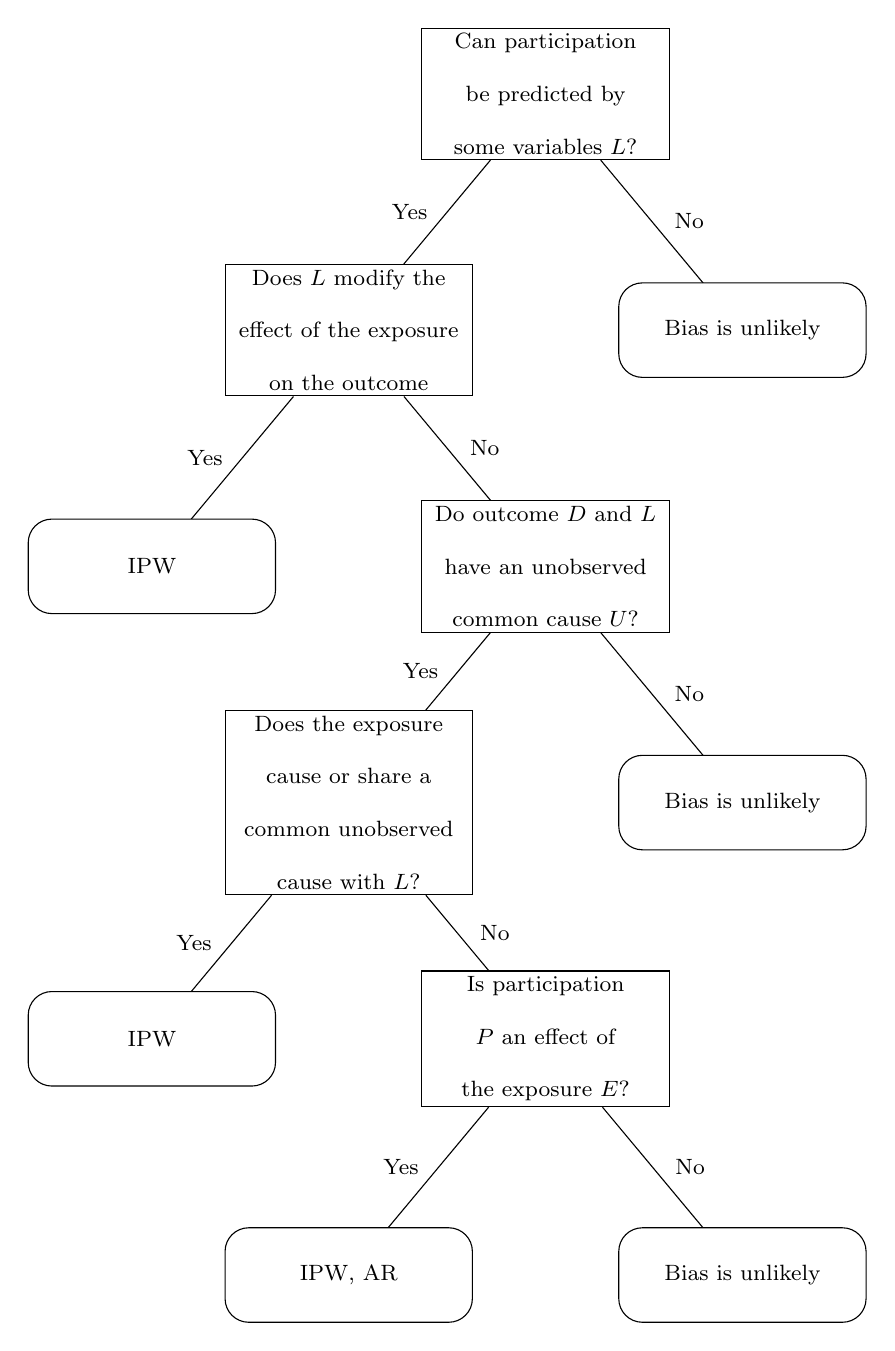
\begin{tikzpicture}
	[
	 sibling distance = 4cm,
	 level distance   = 3cm,
	 every node/.style = {shape=rectangle,
		                  draw,
		                  align=center,
		                  top color = white,
	                      font=\footnotesize,
	                      minimum size = 12mm,
	                      text width = 30mm,
	                      inner sep = 2pt
                         },
    L1/.style = {sibling distance=9cm},
    L2/.style = {sibling distance=5cm},
    L3/.style = {sibling distance=1cm},
    YN/.style = {minimum size = 8mm,
    	         text width = 8mm,
    	         pos = .5,
    	         text opacity = 1,
    	         fill opacity=0}
	]
	
	\newcommand{\LP}{Can participation be predicted by some variables $L$?}
	\newcommand{\nB}{Bias is unlikely}
	\newcommand{\LED}{Does $L$ modify the effect of the exposure
		on the outcome }
	\newcommand{\EL}{Does the exposure cause
		or share a common unobserved
		cause with $L$?}
	\newcommand{\EP}{Is participation $P$
		an effect of
		the exposure $E$?}
	\newcommand{\CCDL}{Do outcome $D$ and $L$
		have an unobserved
		common cause $U$?}	

	\node (A) {\LP}
	child [L2] {[] node  (B1) {\LED}
				child [L2] {[rounded corners=3mm] node (C1) {IPW}}
			    child [L2] {[] node (C2) {\CCDL}
		                    child [L2] {[] node (D1) {\EL}
		                    	        child [L2] {[rounded corners=3mm] node (E1) {IPW}}
		                    	        child [L2] {[] node (E2) {\EP}
		                    	        	        child [L2] {[rounded corners=3mm] node (F1) {IPW, AR}}
		                    	        	        child [L2] {[rounded corners=3mm] node (F2) {\nB}}
		                    	                                      }
		                                                  }
		                    child [L2] {[rounded corners=3mm] node (D2) {\nB}}                    
	                                         }}
	child [L2] {[rounded corners=3mm] node  (B2) {\nB}};
	
	 \begin{scope}[nodes = {draw = none}]
	   \path (A)  -- (B1) node [YN, left]   {Yes};
	   \path (A)  -- (B2) node [YN, right]  {No};
	   \path (B1) -- (C1) node [YN, left]   {Yes};
	   \path (B1) -- (C2) node [YN, right]  {No};
	   \path (C2) -- (D1) node [YN, left]   {Yes};
	   \path (C2) -- (D2) node [YN, right]  {No};
	   \path (D1) -- (E1) node [YN, left]   {Yes};
	   \path (D1) -- (E2) node [YN, right]  {No};
	   \path (E2) -- (F1) node [YN, left]   {Yes};
	   \path (E2) -- (F2) node [YN, right]  {No};
	 \end{scope}
\end{tikzpicture}		
	\end{singlespace}
	
	%
\begin{tikzpicture}
	[
	 sibling distance = 4cm,
	 level distance   = 4cm,
	 every node/.style = {shape=rectangle,
		                  draw,
		                  align=center,
		                  top color = white,
	                      font=\footnotesize,
	                      minimum size = 22mm,
	                      text width = 28mm,
	                      inner sep = 0pt
                         },
    L1/.style ={sibling distance=9cm},
    L2/.style ={sibling distance=5cm},
    L3/.style ={sibling distance=3cm},
    YN/.style = {minimum size = 8mm,
    	text width = 8mm,
    	pos = .5,
    	text opacity = 1,
    	fill opacity=0}
	]
	
	\newcommand{\LP}{Is there a participation indicator $L$?}
	\newcommand{\nB}{Bias is unlikely}
	\newcommand{\LED}{Does $L$ modify the effect of the exposure
		             on the outcome }
	\newcommand{\EL}{Does the expo- sure cause
		             or share a common unobserved
		             cause with $L$?}
    \newcommand{\EP}{Is participation $P$
    	             an effect of
    	             the exposure $E$?}
    \newcommand{\CCDL}{Do outcome $D$ and $L$
    	               have an unobserved
    	               common cause $U$?}	
	\node (A) {\LP}
	child [L2] {[] node  (B1) {\LED}
				child [L1] {[] node (C1) {\EP}
					        child [L2] {[] node (Dx1) {\EL}
					        	        child [L2] {[] node (Ex1) {\CCDL}
					        	        	        child [L2] {[rounded corners=3mm] node (Fx1) {IPPW}}
					        	        	        child [L2] {[rounded corners=3mm] node (Fx2) {DS/MRP, IPPW}}
					        	                                         }
					        	        child [L2] {[rounded corners=3mm] node (Ex2) {DS/MRP, IPPW}}
					                                       }
					        child [L2] {[rounded corners=3mm] node (Dx2) {DS/MRP, IPPW}}
				                              }
			    child [L1] {[] node (C2) {\CCDL}
		                    child [L2] {[] node (D1) {\EL}
		                    	        child [L2] {[rounded corners=3mm] node (E1) {IPPW}}
		                    	        child [L2] {[] node (E2) {\EP}
		                    	        	        child [L2] {[rounded corners=3mm] node (F1) {AR, DS/MRP, IPPW}}
		                    	        	        child [L2] {[rounded corners=3mm] node (F2) {\nB}}
		                    	                                      }
		                                                  }
		                    child [L2] {[rounded corners=3mm] node (D2) {\nB}}                    
	                                         }}
	child [L2] {[rounded corners=3mm] node  (B2) {\nB}};
	
	 \begin{scope}[nodes = {draw = none}]
	   \path (A)  -- (B1) node [YN, left]   {Yes};
	   \path (A)  -- (B2) node [YN, right]  {No};
	   \path (B1) -- (C1) node [YN, left]   {Yes};
	   \path (B1) -- (C2) node [YN, right]  {No};
	   \path (C2) -- (D1) node [YN, left]   {Yes};
	   \path (C2) -- (D2) node [YN, right]  {No};
	   \path (D1) -- (E1) node [YN, left]   {Yes};
	   \path (D1) -- (E2) node [YN, right]  {No};
	   \path (E2) -- (F1) node [YN, left]   {Yes};
	   \path (E2) -- (F2) node [YN, right]  {No};
	   \path (Dx1) -- (Ex1) node [YN, left]   {Yes};
	   \path (Dx1) -- (Ex2) node [YN, right]  {No};
	   \path (C1) -- (Dx1) node [YN, left]   {Yes};
	   \path (C1) -- (Dx2) node [YN, right]  {No};
	   \path (Ex1) -- (Fx1) node [YN, left]   {Yes};
	   \path (Ex1) -- (Fx2) node [YN, right]  {No};
	 \end{scope}
\end{tikzpicture}
	\caption{Decision tree for identification of selection bias and choice of approach to correct for selection bias. See Figure \ref{fig:SelectionBias} for causal diagrams that underlie the decision tree. 
	To determine if selection bias is likely, and if so which correction method can be used, proceed through the questions from the top on. Ending in a node "Bias is unlikely" implies that a standard analysis without correction for selection bias will result in unbiased estimates. Otherwise, different correction types can be used, depending on the underlying causal structure. IPW stands for analysis with inverse probability weighting, AR for adjusted regression. For reasons of brevity, this decision tree does not isolate cases where multilevel regression and post stratification (MRP) can be used to correct bias. See appendix for a more detailed decision tree that represents also these cases.}
	\label{fig:DecisionTree}
\end{figure}


Structural analysis using directed acyclic graphs (DAGs) is a useful tool for the development of analysis strategies that remains underused. A practical argument against the use of DAGs is the uncertainty about causal relationships. We proposed to use genetic correlation coefficients from LD score regression of GWAS summary data as one possibility to substantiate assumptions about unobserved common causes. While unobserved common causes can be of environmental or genetic nature, the main motivation to focus on common genetic causes is the growing availability of large consortium-based GWAS studies---including summary results--- and methodological advances allowing estimation of heritability and genetic correlation coefficients for a diverse set of variables \supercite{Bulik-Sullivan2015-er, Bulik-Sullivan2015-xn}. Because GWAS studies are association studies, they do not provide unambiguous proof for a causal role of genes. Still, even if GWAS associations estimates are partly driven by environmental factors, genetic correlation estimates are of interest because common environmental causes also contribute to the manifestation of selection bias.


A second challenge when using structural models is the difficulty of formulating DAGs for complex causal models\supercite{Shrier2008-vr}. When judging the presence of bias due to self-selection and selective dropout, a simple decision tree can supplant the formulation of a complete DAG, so that the researcher can determine the potential for selection bias by answering a sequence of questions about the relationship of participation indicators, exposures, and outcomes. Figure \ref{fig:DecisionTree} shows a decision tree that can be used to identify when correction for bias is necessary. 

A topic closely related to selection bias is that of the representativeness. While it has been argued that representativeness can be detrimental to scientific inference, because understanding of mechanisms and careful control of relevant variables are central for this aim \supercite{Rothman2013-qc}, others have emphasized the importance of representativeness---understood as the availability of weights for calculating valid population estimates \supercite{Keiding2016-fv}. Careful experimentation based on hypothesized mechanisms is undoubtedly central to scientific inference. Still, this approach does not describe well the often-exploratory analyses of cohort study data. Moreover, if one understands causal inference as the central goal of scientific inquiry, ignoring non-representativeness of unweighted study samples does not only undermine generalization to the population of interest, but can also lead to incorrect scientific inferences by facilitating the "discovery" of associations where there are in fact none, or prevent the detection of existing associations.

In conclusion, self-selection into cohort studies and loss to follow up can lead to biased estimates of exposure outcome associations from large population based cohort studies. Structural analysis and empirical results suggest that especially for mental health related exposures and outcomes selection bias is likely. Still, the dependency of bias on the specific outcome, exposure, and study participation indicators makes general statements about selection bias for multi-exposure multi-outcome studies impossible. Instead, each  investigation of an exposure-outcome association has to assess selection bias. If selection bias is likely and valid participation indicators are available, weighting cases by the inverse of their probability to participate is a robust approach to control bias.

\newpage

\printbibliography

\newpage

\processdelayedfloats

\clearpage

\makeatletter
\efloat@restorefloats
\makeatother

\appendix

\renewcommand{\thefigure}{S\arabic{figure}}
\renewcommand{\thepostfigure}{S\arabic{postfigure}}
\setcounter{figure}{0}
\setcounter{postfigure}{0}

\renewcommand{\thetable}{S\arabic{table}}
\renewcommand{\theposttable}{S\arabic{posttable}}
\setcounter{table}{0}
\setcounter{posttable}{0}

\section{Supplementary Information}

\subsection{Supplementary Methods}

\paragraph{Bayesian regression models.} 
We implemented beta binomial regression models in the probabilistic programming language Stan \supercite{Carpenter2017-gd, Stan_Development_Team2017-lp}. The beta binomal distribution is the natural choice for sum scores as outcome, which are bound between zero and an upper bound. Stan also allows simultaneous estimation of a regression model that uses inverse probability weights (IPW) and one that does not but adjusts for participation indicators (AR), while explicitly modeling the difference (bias) between the models' regression weights.

\paragraph{Comparison of exposure outcome association estimates} The statistical model directly estimates selection bias by modeling regression coefficients for AR as the coefficients for IPW plus the difference between the IPW and the AR coefficients. This approach accounts for covariation between regression weights when estimating bias. The ADHD sum scores are modeled as  $S = beta$-$binomial(\alpha,\beta)$, where $\alpha = \pi\phi$, $\beta = (1-\pi)\phi)$, and phi is the over-dispersion parameter of the beta binomial distribution. The expected sum score is defined as 
\newline
$\mathbf{\pi}_{IPW} = inv.logit(\mathbf{X} \beta_{IPW})$ 
\newline
$\mathbf{\pi}_{AR} = inv.logit(\mathbf{X} \big( \beta_{IPW} + \delta_{AR} \big) + \mathbf{P}\rho)$
\newline
where \textbf{X} is a matrix containing exposures of interest and control variables excluding participation indicators, $\beta_{IPWR}$ are the regression weights for the IPW analysis, $\delta$ models the differences between regression weights for the weighted and adjusted regression, \textbf{P} and $\rho$ are participation indicators and corresponding regression weights.

Because coefficients of a beta-binomial regressions are on the less intuitive multiplicative scale, we used the marginal standardization approach \supercite{Muller2014-bh} to calculate average marginal effects ($AME$), the expected change in the outcome ADHD sum score for a one unit change of the exposure, and report results on this scale.

We test for bias by using a region of practical equivalence approach (ROPE\supercite{Kruschke2010-zi}), which checks if the highest density region of the bias estimates lies within a region of bias magnitudes that is for practical purposes equivalent with zero\supercite{Kruschke2010-zi}. This approach also allows quantifying the risk for substantial bias as the ratio of the posterior probabilities of the bias estimate being inside and outside the ROPE, i.e. $log(RR) = logit(\int_{-b}^{b} \delta)$.

Which range of selection bias can be considered as unproblematic can be judged by subject matter experts. Alternatively, the bias estimate can be standardized by dividing it by the variance of the "gold standard" estimate\supercite{Stuart2010-cj}, here the IPW estimate, which corrects selection bias. A complementary approach is to divide the bias estimate with the mean of the corrected estimate, capturing the intuition that deviations matter less if they are small compared to the corrected estimate. We define the interval of $\pm$ 0.5 standardized deviations as practically equivalent with zero. This sets a high threshold for determining the presence of a problematic bias. In other contexts, different thresholds might be appropriate.

\paragraph{Inverse probability weights} 
Inverse probability weights were calculated based on a hierarchical binomial regression, where participation rates were estimated as an effect of mothers' age, education, and parity,  whereby the intercept as well as linear and non-linear (square) effects of mothers' age were allowed to vary by education and parity. 10-fold cross validation confirmed that this model did not over-fit the data. Following general recommendations we calculated smoothed weights\supercite{Seaman2013-rj}. We calculated weights separately for imputed data sets and used a 2 step approach\supercite{Zigler2016-od} to incorporate uncertainty about weights into the regression analysis.

\paragraph{MCMC estimation} 

Regression models were estimated with Hamiltonian Monte Carlo sampling as implemented in Stan. For each regression, 3 chains were sampled for 20 imputed data sets. Each chain consisted of 250 warmup samples and an additional 500 iterations that were used to calculate statistics. We checked convergence of the 3 chains per imputed data sets by insuring that \^{R} values were below 1.1 \supercite{Gelman1992-jz}, and no divergent transitions had occurred \supercite{Stan_Development_Team2016-pc}. All parameters of all models successfully converged, as indicated by \^{R} values below 1.1. We thus merged all chains prior to calculating statistics\supercite{Zhou2010-li} such that reported results are based on 30,000 (20 imputed data sets $\cdot$ 3 chains $\cdot$ 500 iterations) combined post-warmup samples.

\subsection{Supplementary tables}


\begin{table}[ht]
	\begin{center}
		\begin{tabular}{llr}
			\hline
			Variable group        & Phenotype \& reference           & N \\
			\hline
			Participation         & Years education\cite{Okbay2016-mg} 	   & 292\,000\\
			indicator             & Age at first birth\cite{Barban2016-fa}       & 125\,000\\
			\multicolumn{1}{c}{"} & Nr. children born\cite{Barban2016-fa}       & 125\,000\\
			Exposure              & Birth weight\cite{Horikoshi2016-hq}    & 143\,000\\
			\multicolumn{1}{c}{"} & Ever smoked\cite{Tob_Gen_Cons2010-se} & 75\,000\\
			\multicolumn{1}{c}{"} & Nr. cigarettes per day\cite{Tob_Gen_Cons2010-se} & 75\,000\\
			\multicolumn{1}{c}{"} & Alcohol use\cite{Clarke2017-xz}       & 112\,000\\
			\multicolumn{1}{c}{"} & Lifetime cannabis use\cite{Stringer2016-or}     & 32\,000\\
			\multicolumn{1}{c}{"} & Anxiety\cite{Otowa2016-uo}        & 31\,000\\
			\multicolumn{1}{c}{"} & Depressive symptoms\cite{Okbay2016-pj}        & 161\,000\\
			Outcome               & ADHD diagnosis\cite{Demontis2017-zu}     & 55\,000\\
			\hline
		\end{tabular}
	\end{center}
	\caption{Genome wide association studies on predictors of participation, exposures and outcome.}
	\label{tab:gwas}
\end{table}


% latex table generated in R 3.4.1 by xtable 1.8-2 package
% Fri Mar 23 14:45:43 2018
{
\setlength\tabcolsep{3pt}
\renewcommand{\arraystretch}{0.6}
\begin{longtable}{llrrrrrrrrr}
  \hline
Phenotype 1 & Phenotype 2 & $r_G$ & $se(r_G)$ & $z(r_G)$ & $h^2_{p2}$ & $se(h^2_{p2})$ & $z(h^2_{p2})$ & $h^2_{p1}$ & $se(h^2_{p1})$ & $z(h^2_{p1})$ \\ 
  \hline
  \endhead
ADHD & YearsEdu & -0.54 & 0.03 & -18.4 & 0.12 & \textless 0.00 & 30.2 & 0.23 & 0.01 & 15.5 \\ 
ADHD & AgeFirstBirth & -0.62 & 0.04 & -14.7 & 0.08 & 0.01 & 14.6 & 0.23 & 0.01 & 15.5 \\ 
ADHD & NumChildrBorn & 0.36 & 0.07 & 5.3 & 0.03 & \textless 0.00 & 9.9 & 0.23 & 0.01 & 15.5 \\ 
ADHD & BirthWeight & -0.14 & 0.04 & -3.6 & 0.13 & 0.01 & 15.7 & 0.23 & 0.01 & 15.5 \\ 
ADHD & EverSmoked & 0.49 & 0.06 & 7.9 & 0.08 & 0.01 & 11.4 & 0.23 & 0.01 & 15.5 \\ 
ADHD & CigPerDay & 0.41 & 0.10 & 4.2 & 0.03 & 0.01 & 4.3 & 0.23 & 0.01 & 15.5 \\ 
ADHD & AlcUse & -0.04 & 0.05 & -0.8 & 0.08 & 0.01 & 13.0 & 0.23 & 0.01 & 15.5 \\ 
ADHD & SubstAbuse & 0.63 & 0.04 & 15.0 & 0.02 & \textless 0.00 & 16.4 & 0.23 & 0.01 & 15.5 \\ 
ADHD & DeprSymp & 0.45 & 0.05 & 8.5 & 0.05 & \textless 0.00 & 12.8 & 0.23 & 0.01 & 15.5 \\ 
ADHD & Anxiety & 0.27 & 0.14 & 1.9 & 0.06 & 0.03 & 2.5 & 0.23 & 0.01 & 15.5 \\ 
ADHD & Cannabis & 0.32 & 0.07 & 4.5 & 0.09 & 0.02 & 5.5 & 0.23 & 0.01 & 15.5 \\ 
YearsEdu & AgeFirstBirth & 0.72 & 0.03 & 27.9 & 0.08 & 0.01 & 14.6 & 0.12 & \textless 0.00 & 30.2 \\ 
YearsEdu & NumChildrBorn & -0.23 & 0.04 & -6.0 & 0.03 & \textless 0.00 & 9.9 & 0.12 & \textless 0.00 & 30.2 \\ 
YearsEdu & BirthWeight & 0.11 & 0.03 & 4.3 & 0.13 & 0.01 & 15.7 & 0.12 & \textless 0.00 & 30.2 \\ 
YearsEdu & EverSmoked & -0.35 & 0.04 & -9.1 & 0.08 & 0.01 & 11.4 & 0.12 & \textless 0.00 & 30.2 \\ 
YearsEdu & CigPerDay & -0.26 & 0.06 & -4.3 & 0.03 & 0.01 & 4.3 & 0.12 & \textless 0.00 & 30.2 \\ 
YearsEdu & AlcUse & 0.18 & 0.03 & 5.9 & 0.08 & 0.01 & 13.0 & 0.12 & \textless 0.00 & 30.2 \\ 
YearsEdu & SubstAbuse & -0.53 & 0.03 & -18.0 & 0.02 & \textless 0.00 & 16.4 & 0.12 & \textless 0.00 & 30.2 \\ 
YearsEdu & DeprSymp & -0.33 & 0.04 & -9.0 & 0.05 & \textless 0.00 & 12.8 & 0.12 & \textless 0.00 & 30.2 \\ 
YearsEdu & Anxiety & -0.31 & 0.09 & -3.5 & 0.06 & 0.03 & 2.5 & 0.12 & \textless 0.00 & 30.2 \\ 
YearsEdu & Cannabis & -0.04 & 0.05 & -0.9 & 0.09 & 0.02 & 5.5 & 0.12 & \textless 0.00 & 30.2 \\ 
AgeFirstBirth & NumChildrBorn & -0.65 & 0.05 & -13.6 & 0.03 & \textless 0.00 & 9.9 & 0.08 & 0.01 & 14.6 \\ 
AgeFirstBirth & BirthWeight & 0.10 & 0.04 & 2.5 & 0.13 & 0.01 & 15.7 & 0.08 & 0.01 & 14.6 \\ 
AgeFirstBirth & EverSmoked & -0.37 & 0.05 & -7.3 & 0.08 & 0.01 & 11.4 & 0.08 & 0.01 & 14.6 \\ 
AgeFirstBirth & CigPerDay & -0.46 & 0.10 & -4.6 & 0.03 & 0.01 & 4.3 & 0.08 & 0.01 & 14.6 \\ 
AgeFirstBirth & AlcUse & 0.11 & 0.05 & 2.3 & 0.08 & 0.01 & 13.0 & 0.08 & 0.01 & 14.6 \\ 
AgeFirstBirth & SubstAbuse & -0.62 & 0.05 & -13.4 & 0.02 & \textless 0.00 & 16.4 & 0.08 & 0.01 & 14.6 \\ 
AgeFirstBirth & DeprSymp & -0.34 & 0.05 & -7.4 & 0.05 & \textless 0.00 & 12.8 & 0.08 & 0.01 & 14.6 \\ 
AgeFirstBirth & Anxiety & -0.24 & 0.12 & -2.0 & 0.06 & 0.03 & 2.5 & 0.08 & 0.01 & 14.6 \\ 
AgeFirstBirth & Cannabis & -0.17 & 0.07 & -2.4 & 0.09 & 0.02 & 5.5 & 0.08 & 0.01 & 14.6 \\ 
NumChildrBorn & BirthWeight & -0.03 & 0.05 & -0.5 & 0.13 & 0.01 & 15.7 & 0.03 & \textless 0.00 & 9.9 \\ 
NumChildrBorn & EverSmoked & 0.08 & 0.07 & 1.3 & 0.08 & 0.01 & 11.4 & 0.03 & \textless 0.00 & 9.9 \\ 
NumChildrBorn & CigPerDay & 0.16 & 0.10 & 1.5 & 0.03 & 0.01 & 4.3 & 0.03 & \textless 0.00 & 9.9 \\ 
NumChildrBorn & AlcUse & 0.06 & 0.06 & 1.0 & 0.08 & 0.01 & 13.0 & 0.03 & \textless 0.00 & 9.9 \\ 
NumChildrBorn & SubstAbuse & 0.33 & 0.06 & 5.6 & 0.02 & \textless 0.00 & 16.4 & 0.03 & \textless 0.00 & 9.9 \\ 
NumChildrBorn & DeprSymp & 0.19 & 0.07 & 2.9 & 0.05 & \textless 0.00 & 12.8 & 0.03 & \textless 0.00 & 9.9 \\ 
NumChildrBorn & Anxiety & 0.20 & 0.17 & 1.2 & 0.06 & 0.03 & 2.5 & 0.03 & \textless 0.00 & 9.9 \\ 
NumChildrBorn & Cannabis & 0.05 & 0.10 & 0.5 & 0.09 & 0.02 & 5.5 & 0.03 & \textless 0.00 & 9.9 \\ 
BirthWeight & EverSmoked & 0.01 & 0.04 & 0.1 & 0.08 & 0.01 & 11.4 & 0.13 & 0.01 & 15.7 \\ 
BirthWeight & CigPerDay & -0.04 & 0.06 & -0.7 & 0.03 & 0.01 & 4.3 & 0.13 & 0.01 & 15.7 \\ 
BirthWeight & AlcUse & -0.06 & 0.04 & -1.3 & 0.08 & 0.01 & 13.0 & 0.13 & 0.01 & 15.7 \\ 
BirthWeight & SubstAbuse & -0.18 & 0.04 & -4.9 & 0.02 & \textless 0.00 & 16.4 & 0.13 & 0.01 & 15.7 \\ 
BirthWeight & DeprSymp & -0.07 & 0.04 & -1.7 & 0.05 & \textless 0.00 & 12.8 & 0.13 & 0.01 & 15.7 \\ 
BirthWeight & Anxiety & -0.07 & 0.11 & -0.7 & 0.06 & 0.03 & 2.5 & 0.13 & 0.01 & 15.7 \\ 
BirthWeight & Cannabis & -0.02 & 0.07 & -0.3 & 0.09 & 0.02 & 5.5 & 0.13 & 0.01 & 15.7 \\ 
EverSmoked & CigPerDay & 0.37 & 0.11 & 3.5 & 0.03 & 0.01 & 4.3 & 0.08 & 0.01 & 11.4 \\ 
EverSmoked & AlcUse & 0.40 & 0.06 & 6.3 & 0.08 & 0.01 & 13.0 & 0.08 & 0.01 & 11.4 \\ 
EverSmoked & SubstAbuse & 0.60 & 0.05 & 11.6 & 0.02 & \textless 0.00 & 16.4 & 0.08 & 0.01 & 11.4 \\ 
EverSmoked & DeprSymp & 0.25 & 0.06 & 4.4 & 0.05 & \textless 0.00 & 12.8 & 0.08 & 0.01 & 11.4 \\ 
EverSmoked & Anxiety & 0.58 & 0.16 & 3.5 & 0.06 & 0.03 & 2.5 & 0.08 & 0.01 & 11.4 \\ 
EverSmoked & Cannabis & 0.68 & 0.10 & 6.5 & 0.09 & 0.02 & 5.5 & 0.08 & 0.01 & 11.4 \\ 
CigPerDay & AlcUse & -0.10 & 0.09 & -1.1 & 0.08 & 0.01 & 13.0 & 0.03 & 0.01 & 4.3 \\ 
CigPerDay & SubstAbuse & 0.50 & 0.08 & 5.9 & 0.02 & \textless 0.00 & 16.4 & 0.03 & 0.01 & 4.3 \\ 
CigPerDay & DeprSymp & 0.26 & 0.09 & 3.0 & 0.05 & \textless 0.00 & 12.8 & 0.03 & 0.01 & 4.3 \\ 
CigPerDay & Anxiety & -0.03 & 0.20 & -0.2 & 0.06 & 0.03 & 2.5 & 0.03 & 0.01 & 4.3 \\ 
CigPerDay & Cannabis & 0.07 & 0.13 & 0.6 & 0.09 & 0.02 & 5.5 & 0.03 & 0.01 & 4.3 \\ 
AlcUse & SubstAbuse & 0.18 & 0.05 & 3.9 & 0.02 & \textless 0.00 & 16.4 & 0.08 & 0.01 & 13.0 \\ 
AlcUse & DeprSymp & -0.16 & 0.06 & -2.8 & 0.05 & \textless 0.00 & 12.8 & 0.08 & 0.01 & 13.0 \\ 
AlcUse & Anxiety & 0.05 & 0.12 & 0.4 & 0.06 & 0.03 & 2.5 & 0.08 & 0.01 & 13.0 \\ 
AlcUse & Cannabis & 0.39 & 0.08 & 4.8 & 0.09 & 0.02 & 5.5 & 0.08 & 0.01 & 13.0 \\ 
SubstAbuse & DeprSymp & 0.50 & 0.06 & 9.1 & 0.05 & \textless 0.00 & 12.8 & 0.02 & \textless 0.00 & 16.4 \\ 
SubstAbuse & Anxiety & 0.31 & 0.13 & 2.5 & 0.06 & 0.03 & 2.5 & 0.02 & \textless 0.00 & 16.4 \\ 
SubstAbuse & Cannabis & 0.30 & 0.08 & 4.0 & 0.09 & 0.02 & 5.5 & 0.02 & \textless 0.00 & 16.4 \\ 
DeprSymp & Anxiety & 0.65 & 0.17 & 3.9 & 0.06 & 0.03 & 2.5 & 0.05 & \textless 0.00 & 12.8 \\ 
DeprSymp & Cannabis & 0.25 & 0.08 & 2.9 & 0.09 & 0.02 & 5.5 & 0.05 & \textless 0.00 & 12.8 \\ 
Anxiety & Cannabis & -0.05 & 0.18 & -0.3 & 0.09 & 0.02 & 5.5 & 0.06 & 0.03 & 2.5 \\ 
  \hline
\caption{SNP based genetic correlations and heritability estimates from publicly available GWAS summary statistics.} 
\label{tab:rg}
\end{longtable}
\renewcommand{\arraystretch}{1}
}

\newpage

\subsection{Supplementary figures}

%\begin{figure}[ht]
%	\centering
%	% Created by tikzDevice version 0.11 on 2018-03-23 13:16:34
% !TEX encoding = UTF-8 Unicode
\begin{tikzpicture}[x=1pt,y=1pt]
\definecolor{fillColor}{RGB}{255,255,255}
\path[use as bounding box,fill=fillColor,fill opacity=0.00] (0,0) rectangle (341.43,199.17);
\begin{scope}
\path[clip] (  0.00,  0.00) rectangle (341.43,199.17);
\definecolor{drawColor}{RGB}{0,0,0}

\node[text=drawColor,anchor=base,inner sep=0pt, outer sep=0pt, scale=  1.00] at (182.72,  2.40) {ADHD sum score};

\node[text=drawColor,rotate= 90.00,anchor=base,inner sep=0pt, outer sep=0pt, scale=  1.00] at (  9.60,117.58) {Frequency};
\end{scope}
\begin{scope}
\path[clip] (  0.00,  0.00) rectangle (341.43,199.17);
\definecolor{drawColor}{RGB}{0,0,0}

\path[draw=drawColor,line width= 0.4pt,line join=round,line cap=round] ( 52.77, 36.00) -- (289.03, 36.00);

\path[draw=drawColor,line width= 0.4pt,line join=round,line cap=round] ( 52.77, 36.00) -- ( 52.77, 34.37);

\path[draw=drawColor,line width= 0.4pt,line join=round,line cap=round] (111.84, 36.00) -- (111.84, 34.37);

\path[draw=drawColor,line width= 0.4pt,line join=round,line cap=round] (170.90, 36.00) -- (170.90, 34.37);

\path[draw=drawColor,line width= 0.4pt,line join=round,line cap=round] (229.97, 36.00) -- (229.97, 34.37);

\path[draw=drawColor,line width= 0.4pt,line join=round,line cap=round] (289.03, 36.00) -- (289.03, 34.37);

\node[text=drawColor,anchor=base,inner sep=0pt, outer sep=0pt, scale=  1.00] at ( 52.77, 18.00) {0};

\node[text=drawColor,anchor=base,inner sep=0pt, outer sep=0pt, scale=  1.00] at (111.84, 18.00) {5};

\node[text=drawColor,anchor=base,inner sep=0pt, outer sep=0pt, scale=  1.00] at (170.90, 18.00) {10};

\node[text=drawColor,anchor=base,inner sep=0pt, outer sep=0pt, scale=  1.00] at (229.97, 18.00) {15};

\node[text=drawColor,anchor=base,inner sep=0pt, outer sep=0pt, scale=  1.00] at (289.03, 18.00) {20};

\path[draw=drawColor,line width= 0.4pt,line join=round,line cap=round] ( 36.00, 42.04) -- ( 36.00,185.45);

\path[draw=drawColor,line width= 0.4pt,line join=round,line cap=round] ( 36.00, 42.04) -- ( 34.37, 42.04);

\path[draw=drawColor,line width= 0.4pt,line join=round,line cap=round] ( 36.00, 65.95) -- ( 34.37, 65.95);

\path[draw=drawColor,line width= 0.4pt,line join=round,line cap=round] ( 36.00, 89.85) -- ( 34.37, 89.85);

\path[draw=drawColor,line width= 0.4pt,line join=round,line cap=round] ( 36.00,113.75) -- ( 34.37,113.75);

\path[draw=drawColor,line width= 0.4pt,line join=round,line cap=round] ( 36.00,137.65) -- ( 34.37,137.65);

\path[draw=drawColor,line width= 0.4pt,line join=round,line cap=round] ( 36.00,161.55) -- ( 34.37,161.55);

\path[draw=drawColor,line width= 0.4pt,line join=round,line cap=round] ( 36.00,185.45) -- ( 34.37,185.45);

\node[text=drawColor,rotate= 90.00,anchor=base,inner sep=0pt, outer sep=0pt, scale=  1.00] at ( 25.20, 42.04) {0};

\node[text=drawColor,rotate= 90.00,anchor=base,inner sep=0pt, outer sep=0pt, scale=  1.00] at ( 25.20, 65.95) {1000};

\node[text=drawColor,rotate= 90.00,anchor=base,inner sep=0pt, outer sep=0pt, scale=  1.00] at ( 25.20,113.75) {3000};

\node[text=drawColor,rotate= 90.00,anchor=base,inner sep=0pt, outer sep=0pt, scale=  1.00] at ( 25.20,161.55) {5000};
\end{scope}
\begin{scope}
\path[clip] ( 36.00, 36.00) rectangle (329.43,199.17);
\definecolor{drawColor}{RGB}{0,0,0}

\path[draw=drawColor,line width= 0.4pt,line join=round,line cap=round] ( 46.87, 42.04) rectangle ( 58.68, 76.94);

\path[draw=drawColor,line width= 0.4pt,line join=round,line cap=round] ( 58.68, 42.04) rectangle ( 70.49,110.04);

\path[draw=drawColor,line width= 0.4pt,line join=round,line cap=round] ( 70.49, 42.04) rectangle ( 82.31,134.81);

\path[draw=drawColor,line width= 0.4pt,line join=round,line cap=round] ( 82.31, 42.04) rectangle ( 94.12,156.84);

\path[draw=drawColor,line width= 0.4pt,line join=round,line cap=round] ( 94.12, 42.04) rectangle (105.93,177.66);

\path[draw=drawColor,line width= 0.4pt,line join=round,line cap=round] (105.93, 42.04) rectangle (117.75,193.13);

\path[draw=drawColor,line width= 0.4pt,line join=round,line cap=round] (117.75, 42.04) rectangle (129.56,185.84);

\path[draw=drawColor,line width= 0.4pt,line join=round,line cap=round] (129.56, 42.04) rectangle (141.37,180.17);

\path[draw=drawColor,line width= 0.4pt,line join=round,line cap=round] (141.37, 42.04) rectangle (153.18,166.52);

\path[draw=drawColor,line width= 0.4pt,line join=round,line cap=round] (153.18, 42.04) rectangle (165.00,142.81);

\path[draw=drawColor,line width= 0.4pt,line join=round,line cap=round] (165.00, 42.04) rectangle (176.81,122.40);

\path[draw=drawColor,line width= 0.4pt,line join=round,line cap=round] (176.81, 42.04) rectangle (188.62,102.59);

\path[draw=drawColor,line width= 0.4pt,line join=round,line cap=round] (188.62, 42.04) rectangle (200.44, 85.33);

\path[draw=drawColor,line width= 0.4pt,line join=round,line cap=round] (200.44, 42.04) rectangle (212.25, 73.47);

\path[draw=drawColor,line width= 0.4pt,line join=round,line cap=round] (212.25, 42.04) rectangle (224.06, 60.85);

\path[draw=drawColor,line width= 0.4pt,line join=round,line cap=round] (224.06, 42.04) rectangle (235.87, 54.76);

\path[draw=drawColor,line width= 0.4pt,line join=round,line cap=round] (235.87, 42.04) rectangle (247.69, 51.48);

\path[draw=drawColor,line width= 0.4pt,line join=round,line cap=round] (247.69, 42.04) rectangle (259.50, 47.68);

\path[draw=drawColor,line width= 0.4pt,line join=round,line cap=round] (259.50, 42.04) rectangle (271.31, 45.41);

\path[draw=drawColor,line width= 0.4pt,line join=round,line cap=round] (271.31, 42.04) rectangle (283.13, 44.00);

\path[draw=drawColor,line width= 0.4pt,line join=round,line cap=round] (283.13, 42.04) rectangle (294.94, 43.07);

\path[draw=drawColor,line width= 0.4pt,line join=round,line cap=round] (294.94, 42.04) rectangle (306.75, 42.57);

\path[draw=drawColor,line width= 0.4pt,line join=round,line cap=round] (306.75, 42.04) rectangle (318.57, 42.19);
\end{scope}
\end{tikzpicture}

%	\caption{\footnotesize Distribution of ADHD sum score calculated from mother reported ADHD symptoms.}
%	\label{fig:ADHDsumscore}
%\end{figure}

\begin{figure}[ht]
	\centering % Created by tikzDevice version 0.11 on 2018-03-23 10:53:14
% !TEX encoding = UTF-8 Unicode
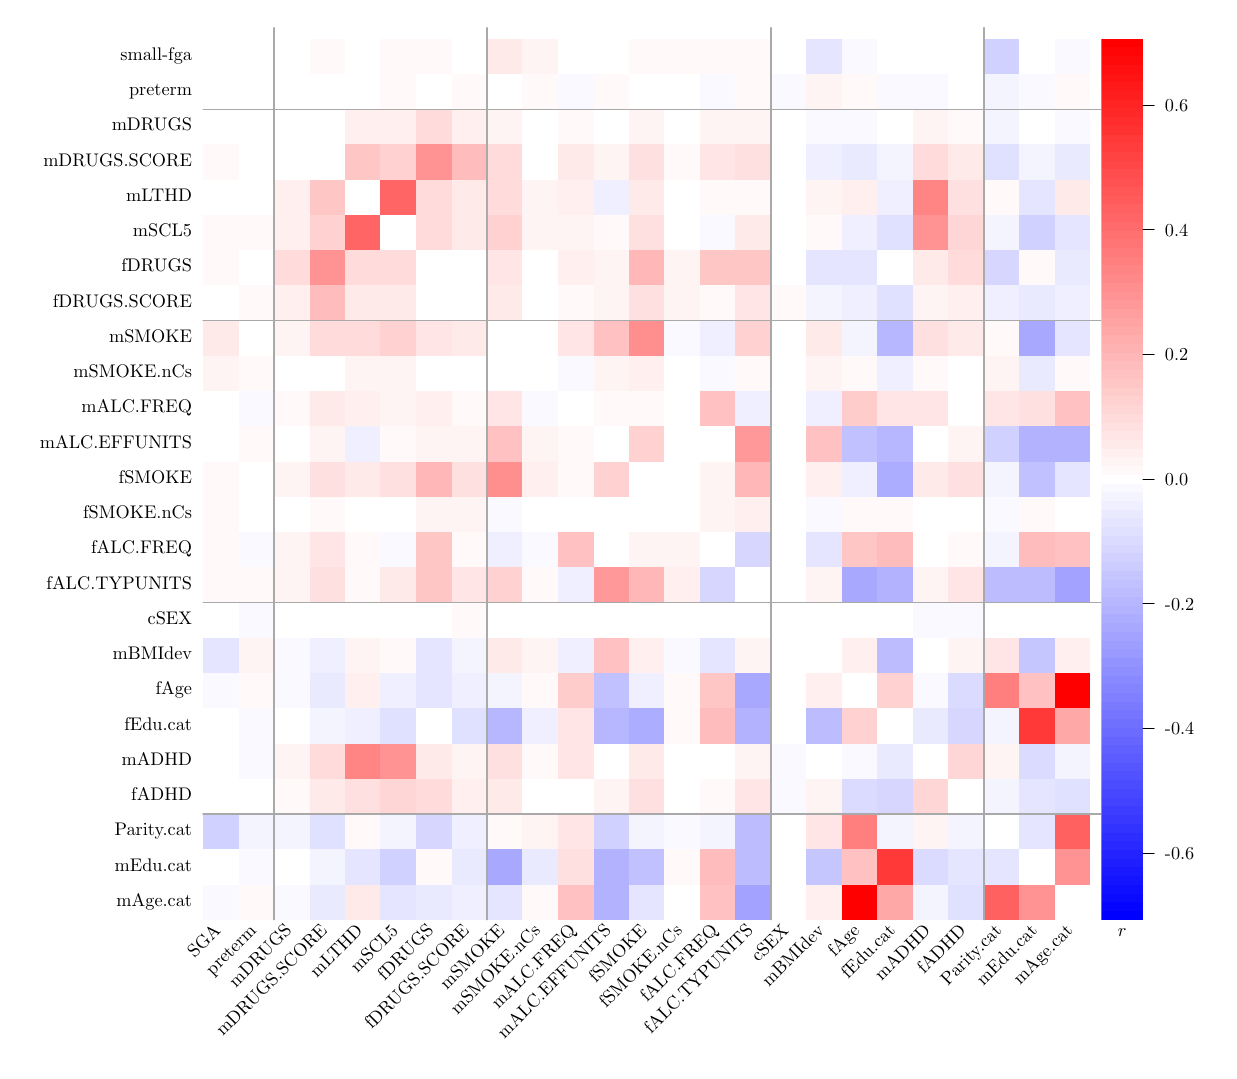
\begin{tikzpicture}[x=1pt,y=1pt]
\definecolor{fillColor}{RGB}{255,255,255}
\path[use as bounding box,fill=fillColor,fill opacity=0.00] (0,0) rectangle (426.79,369.89);
\begin{scope}
\path[clip] ( 63.36, 47.52) rectangle (384.03,365.93);
\definecolor{fillColor}{RGB}{249,249,255}

\path[fill=fillColor] ( 63.36, 47.52) rectangle ( 76.19, 60.26);
\definecolor{fillColor}{RGB}{255,255,255}

\path[fill=fillColor] ( 63.36, 60.26) rectangle ( 76.19, 72.99);
\definecolor{fillColor}{RGB}{209,209,255}

\path[fill=fillColor] ( 63.36, 72.99) rectangle ( 76.19, 85.73);
\definecolor{fillColor}{RGB}{255,255,255}

\path[fill=fillColor] ( 63.36, 85.73) rectangle ( 76.19, 98.46);

\path[fill=fillColor] ( 63.36, 98.46) rectangle ( 76.19,111.20);

\path[fill=fillColor] ( 63.36,111.20) rectangle ( 76.19,123.94);
\definecolor{fillColor}{RGB}{249,249,255}

\path[fill=fillColor] ( 63.36,123.94) rectangle ( 76.19,136.67);
\definecolor{fillColor}{RGB}{229,229,255}

\path[fill=fillColor] ( 63.36,136.67) rectangle ( 76.19,149.41);
\definecolor{fillColor}{RGB}{255,255,255}

\path[fill=fillColor] ( 63.36,149.41) rectangle ( 76.19,162.15);
\definecolor{fillColor}{RGB}{255,249,249}

\path[fill=fillColor] ( 63.36,162.15) rectangle ( 76.19,174.88);

\path[fill=fillColor] ( 63.36,174.88) rectangle ( 76.19,187.62);

\path[fill=fillColor] ( 63.36,187.62) rectangle ( 76.19,200.35);

\path[fill=fillColor] ( 63.36,200.35) rectangle ( 76.19,213.09);
\definecolor{fillColor}{RGB}{255,255,255}

\path[fill=fillColor] ( 63.36,213.09) rectangle ( 76.19,225.83);

\path[fill=fillColor] ( 63.36,225.83) rectangle ( 76.19,238.56);
\definecolor{fillColor}{RGB}{255,244,244}

\path[fill=fillColor] ( 63.36,238.56) rectangle ( 76.19,251.30);
\definecolor{fillColor}{RGB}{255,234,234}

\path[fill=fillColor] ( 63.36,251.30) rectangle ( 76.19,264.04);
\definecolor{fillColor}{RGB}{255,255,255}

\path[fill=fillColor] ( 63.36,264.04) rectangle ( 76.19,276.77);
\definecolor{fillColor}{RGB}{255,249,249}

\path[fill=fillColor] ( 63.36,276.77) rectangle ( 76.19,289.51);

\path[fill=fillColor] ( 63.36,289.51) rectangle ( 76.19,302.24);
\definecolor{fillColor}{RGB}{255,255,255}

\path[fill=fillColor] ( 63.36,302.24) rectangle ( 76.19,314.98);
\definecolor{fillColor}{RGB}{255,249,249}

\path[fill=fillColor] ( 63.36,314.98) rectangle ( 76.19,327.72);
\definecolor{fillColor}{RGB}{255,255,255}

\path[fill=fillColor] ( 63.36,327.72) rectangle ( 76.19,340.45);

\path[fill=fillColor] ( 63.36,340.45) rectangle ( 76.19,353.19);
\definecolor{fillColor}{RGB}{255,249,249}

\path[fill=fillColor] ( 76.19, 47.52) rectangle ( 89.01, 60.26);
\definecolor{fillColor}{RGB}{249,249,255}

\path[fill=fillColor] ( 76.19, 60.26) rectangle ( 89.01, 72.99);
\definecolor{fillColor}{RGB}{244,244,255}

\path[fill=fillColor] ( 76.19, 72.99) rectangle ( 89.01, 85.73);
\definecolor{fillColor}{RGB}{255,255,255}

\path[fill=fillColor] ( 76.19, 85.73) rectangle ( 89.01, 98.46);
\definecolor{fillColor}{RGB}{249,249,255}

\path[fill=fillColor] ( 76.19, 98.46) rectangle ( 89.01,111.20);

\path[fill=fillColor] ( 76.19,111.20) rectangle ( 89.01,123.94);
\definecolor{fillColor}{RGB}{255,249,249}

\path[fill=fillColor] ( 76.19,123.94) rectangle ( 89.01,136.67);
\definecolor{fillColor}{RGB}{255,244,244}

\path[fill=fillColor] ( 76.19,136.67) rectangle ( 89.01,149.41);
\definecolor{fillColor}{RGB}{249,249,255}

\path[fill=fillColor] ( 76.19,149.41) rectangle ( 89.01,162.15);
\definecolor{fillColor}{RGB}{255,249,249}

\path[fill=fillColor] ( 76.19,162.15) rectangle ( 89.01,174.88);
\definecolor{fillColor}{RGB}{249,249,255}

\path[fill=fillColor] ( 76.19,174.88) rectangle ( 89.01,187.62);
\definecolor{fillColor}{RGB}{255,255,255}

\path[fill=fillColor] ( 76.19,187.62) rectangle ( 89.01,200.35);

\path[fill=fillColor] ( 76.19,200.35) rectangle ( 89.01,213.09);
\definecolor{fillColor}{RGB}{255,249,249}

\path[fill=fillColor] ( 76.19,213.09) rectangle ( 89.01,225.83);
\definecolor{fillColor}{RGB}{249,249,255}

\path[fill=fillColor] ( 76.19,225.83) rectangle ( 89.01,238.56);
\definecolor{fillColor}{RGB}{255,249,249}

\path[fill=fillColor] ( 76.19,238.56) rectangle ( 89.01,251.30);
\definecolor{fillColor}{RGB}{255,255,255}

\path[fill=fillColor] ( 76.19,251.30) rectangle ( 89.01,264.04);
\definecolor{fillColor}{RGB}{255,249,249}

\path[fill=fillColor] ( 76.19,264.04) rectangle ( 89.01,276.77);
\definecolor{fillColor}{RGB}{255,255,255}

\path[fill=fillColor] ( 76.19,276.77) rectangle ( 89.01,289.51);
\definecolor{fillColor}{RGB}{255,249,249}

\path[fill=fillColor] ( 76.19,289.51) rectangle ( 89.01,302.24);
\definecolor{fillColor}{RGB}{255,255,255}

\path[fill=fillColor] ( 76.19,302.24) rectangle ( 89.01,314.98);

\path[fill=fillColor] ( 76.19,314.98) rectangle ( 89.01,327.72);

\path[fill=fillColor] ( 76.19,327.72) rectangle ( 89.01,340.45);

\path[fill=fillColor] ( 76.19,353.19) rectangle ( 89.01,365.93);
\definecolor{fillColor}{RGB}{249,249,255}

\path[fill=fillColor] ( 89.01, 47.52) rectangle (101.84, 60.26);
\definecolor{fillColor}{RGB}{255,255,255}

\path[fill=fillColor] ( 89.01, 60.26) rectangle (101.84, 72.99);
\definecolor{fillColor}{RGB}{244,244,255}

\path[fill=fillColor] ( 89.01, 72.99) rectangle (101.84, 85.73);
\definecolor{fillColor}{RGB}{255,249,249}

\path[fill=fillColor] ( 89.01, 85.73) rectangle (101.84, 98.46);
\definecolor{fillColor}{RGB}{255,244,244}

\path[fill=fillColor] ( 89.01, 98.46) rectangle (101.84,111.20);
\definecolor{fillColor}{RGB}{255,255,255}

\path[fill=fillColor] ( 89.01,111.20) rectangle (101.84,123.94);
\definecolor{fillColor}{RGB}{249,249,255}

\path[fill=fillColor] ( 89.01,123.94) rectangle (101.84,136.67);

\path[fill=fillColor] ( 89.01,136.67) rectangle (101.84,149.41);
\definecolor{fillColor}{RGB}{255,255,255}

\path[fill=fillColor] ( 89.01,149.41) rectangle (101.84,162.15);
\definecolor{fillColor}{RGB}{255,244,244}

\path[fill=fillColor] ( 89.01,162.15) rectangle (101.84,174.88);

\path[fill=fillColor] ( 89.01,174.88) rectangle (101.84,187.62);
\definecolor{fillColor}{RGB}{255,255,255}

\path[fill=fillColor] ( 89.01,187.62) rectangle (101.84,200.35);
\definecolor{fillColor}{RGB}{255,244,244}

\path[fill=fillColor] ( 89.01,200.35) rectangle (101.84,213.09);
\definecolor{fillColor}{RGB}{255,255,255}

\path[fill=fillColor] ( 89.01,213.09) rectangle (101.84,225.83);
\definecolor{fillColor}{RGB}{255,249,249}

\path[fill=fillColor] ( 89.01,225.83) rectangle (101.84,238.56);
\definecolor{fillColor}{RGB}{255,255,255}

\path[fill=fillColor] ( 89.01,238.56) rectangle (101.84,251.30);
\definecolor{fillColor}{RGB}{255,244,244}

\path[fill=fillColor] ( 89.01,251.30) rectangle (101.84,264.04);
\definecolor{fillColor}{RGB}{255,239,239}

\path[fill=fillColor] ( 89.01,264.04) rectangle (101.84,276.77);
\definecolor{fillColor}{RGB}{255,219,219}

\path[fill=fillColor] ( 89.01,276.77) rectangle (101.84,289.51);
\definecolor{fillColor}{RGB}{255,239,239}

\path[fill=fillColor] ( 89.01,289.51) rectangle (101.84,302.24);

\path[fill=fillColor] ( 89.01,302.24) rectangle (101.84,314.98);
\definecolor{fillColor}{RGB}{255,255,255}

\path[fill=fillColor] ( 89.01,314.98) rectangle (101.84,327.72);

\path[fill=fillColor] ( 89.01,340.45) rectangle (101.84,353.19);

\path[fill=fillColor] ( 89.01,353.19) rectangle (101.84,365.93);
\definecolor{fillColor}{RGB}{234,234,255}

\path[fill=fillColor] (101.84, 47.52) rectangle (114.67, 60.26);
\definecolor{fillColor}{RGB}{244,244,255}

\path[fill=fillColor] (101.84, 60.26) rectangle (114.67, 72.99);
\definecolor{fillColor}{RGB}{224,224,255}

\path[fill=fillColor] (101.84, 72.99) rectangle (114.67, 85.73);
\definecolor{fillColor}{RGB}{255,234,234}

\path[fill=fillColor] (101.84, 85.73) rectangle (114.67, 98.46);
\definecolor{fillColor}{RGB}{255,219,219}

\path[fill=fillColor] (101.84, 98.46) rectangle (114.67,111.20);
\definecolor{fillColor}{RGB}{244,244,255}

\path[fill=fillColor] (101.84,111.20) rectangle (114.67,123.94);
\definecolor{fillColor}{RGB}{234,234,255}

\path[fill=fillColor] (101.84,123.94) rectangle (114.67,136.67);
\definecolor{fillColor}{RGB}{239,239,255}

\path[fill=fillColor] (101.84,136.67) rectangle (114.67,149.41);
\definecolor{fillColor}{RGB}{255,255,255}

\path[fill=fillColor] (101.84,149.41) rectangle (114.67,162.15);
\definecolor{fillColor}{RGB}{255,224,224}

\path[fill=fillColor] (101.84,162.15) rectangle (114.67,174.88);
\definecolor{fillColor}{RGB}{255,229,229}

\path[fill=fillColor] (101.84,174.88) rectangle (114.67,187.62);
\definecolor{fillColor}{RGB}{255,249,249}

\path[fill=fillColor] (101.84,187.62) rectangle (114.67,200.35);
\definecolor{fillColor}{RGB}{255,224,224}

\path[fill=fillColor] (101.84,200.35) rectangle (114.67,213.09);
\definecolor{fillColor}{RGB}{255,244,244}

\path[fill=fillColor] (101.84,213.09) rectangle (114.67,225.83);
\definecolor{fillColor}{RGB}{255,234,234}

\path[fill=fillColor] (101.84,225.83) rectangle (114.67,238.56);
\definecolor{fillColor}{RGB}{255,255,255}

\path[fill=fillColor] (101.84,238.56) rectangle (114.67,251.30);
\definecolor{fillColor}{RGB}{255,219,219}

\path[fill=fillColor] (101.84,251.30) rectangle (114.67,264.04);
\definecolor{fillColor}{RGB}{255,188,188}

\path[fill=fillColor] (101.84,264.04) rectangle (114.67,276.77);
\definecolor{fillColor}{RGB}{255,147,147}

\path[fill=fillColor] (101.84,276.77) rectangle (114.67,289.51);
\definecolor{fillColor}{RGB}{255,209,209}

\path[fill=fillColor] (101.84,289.51) rectangle (114.67,302.24);
\definecolor{fillColor}{RGB}{255,198,198}

\path[fill=fillColor] (101.84,302.24) rectangle (114.67,314.98);
\definecolor{fillColor}{RGB}{255,255,255}

\path[fill=fillColor] (101.84,327.72) rectangle (114.67,340.45);

\path[fill=fillColor] (101.84,340.45) rectangle (114.67,353.19);
\definecolor{fillColor}{RGB}{255,249,249}

\path[fill=fillColor] (101.84,353.19) rectangle (114.67,365.93);
\definecolor{fillColor}{RGB}{255,234,234}

\path[fill=fillColor] (114.67, 47.52) rectangle (127.49, 60.26);
\definecolor{fillColor}{RGB}{229,229,255}

\path[fill=fillColor] (114.67, 60.26) rectangle (127.49, 72.99);
\definecolor{fillColor}{RGB}{255,249,249}

\path[fill=fillColor] (114.67, 72.99) rectangle (127.49, 85.73);
\definecolor{fillColor}{RGB}{255,224,224}

\path[fill=fillColor] (114.67, 85.73) rectangle (127.49, 98.46);
\definecolor{fillColor}{RGB}{255,132,132}

\path[fill=fillColor] (114.67, 98.46) rectangle (127.49,111.20);
\definecolor{fillColor}{RGB}{239,239,255}

\path[fill=fillColor] (114.67,111.20) rectangle (127.49,123.94);
\definecolor{fillColor}{RGB}{255,239,239}

\path[fill=fillColor] (114.67,123.94) rectangle (127.49,136.67);
\definecolor{fillColor}{RGB}{255,244,244}

\path[fill=fillColor] (114.67,136.67) rectangle (127.49,149.41);
\definecolor{fillColor}{RGB}{255,255,255}

\path[fill=fillColor] (114.67,149.41) rectangle (127.49,162.15);
\definecolor{fillColor}{RGB}{255,249,249}

\path[fill=fillColor] (114.67,162.15) rectangle (127.49,174.88);

\path[fill=fillColor] (114.67,174.88) rectangle (127.49,187.62);
\definecolor{fillColor}{RGB}{255,255,255}

\path[fill=fillColor] (114.67,187.62) rectangle (127.49,200.35);
\definecolor{fillColor}{RGB}{255,234,234}

\path[fill=fillColor] (114.67,200.35) rectangle (127.49,213.09);
\definecolor{fillColor}{RGB}{239,239,255}

\path[fill=fillColor] (114.67,213.09) rectangle (127.49,225.83);
\definecolor{fillColor}{RGB}{255,239,239}

\path[fill=fillColor] (114.67,225.83) rectangle (127.49,238.56);
\definecolor{fillColor}{RGB}{255,244,244}

\path[fill=fillColor] (114.67,238.56) rectangle (127.49,251.30);
\definecolor{fillColor}{RGB}{255,219,219}

\path[fill=fillColor] (114.67,251.30) rectangle (127.49,264.04);
\definecolor{fillColor}{RGB}{255,234,234}

\path[fill=fillColor] (114.67,264.04) rectangle (127.49,276.77);
\definecolor{fillColor}{RGB}{255,219,219}

\path[fill=fillColor] (114.67,276.77) rectangle (127.49,289.51);
\definecolor{fillColor}{RGB}{255,101,101}

\path[fill=fillColor] (114.67,289.51) rectangle (127.49,302.24);
\definecolor{fillColor}{RGB}{255,198,198}

\path[fill=fillColor] (114.67,314.98) rectangle (127.49,327.72);
\definecolor{fillColor}{RGB}{255,239,239}

\path[fill=fillColor] (114.67,327.72) rectangle (127.49,340.45);
\definecolor{fillColor}{RGB}{255,255,255}

\path[fill=fillColor] (114.67,340.45) rectangle (127.49,353.19);

\path[fill=fillColor] (114.67,353.19) rectangle (127.49,365.93);
\definecolor{fillColor}{RGB}{229,229,255}

\path[fill=fillColor] (127.49, 47.52) rectangle (140.32, 60.26);
\definecolor{fillColor}{RGB}{209,209,255}

\path[fill=fillColor] (127.49, 60.26) rectangle (140.32, 72.99);
\definecolor{fillColor}{RGB}{244,244,255}

\path[fill=fillColor] (127.49, 72.99) rectangle (140.32, 85.73);
\definecolor{fillColor}{RGB}{255,214,214}

\path[fill=fillColor] (127.49, 85.73) rectangle (140.32, 98.46);
\definecolor{fillColor}{RGB}{255,147,147}

\path[fill=fillColor] (127.49, 98.46) rectangle (140.32,111.20);
\definecolor{fillColor}{RGB}{224,224,255}

\path[fill=fillColor] (127.49,111.20) rectangle (140.32,123.94);
\definecolor{fillColor}{RGB}{239,239,255}

\path[fill=fillColor] (127.49,123.94) rectangle (140.32,136.67);
\definecolor{fillColor}{RGB}{255,249,249}

\path[fill=fillColor] (127.49,136.67) rectangle (140.32,149.41);
\definecolor{fillColor}{RGB}{255,255,255}

\path[fill=fillColor] (127.49,149.41) rectangle (140.32,162.15);
\definecolor{fillColor}{RGB}{255,234,234}

\path[fill=fillColor] (127.49,162.15) rectangle (140.32,174.88);
\definecolor{fillColor}{RGB}{249,249,255}

\path[fill=fillColor] (127.49,174.88) rectangle (140.32,187.62);
\definecolor{fillColor}{RGB}{255,255,255}

\path[fill=fillColor] (127.49,187.62) rectangle (140.32,200.35);
\definecolor{fillColor}{RGB}{255,224,224}

\path[fill=fillColor] (127.49,200.35) rectangle (140.32,213.09);
\definecolor{fillColor}{RGB}{255,249,249}

\path[fill=fillColor] (127.49,213.09) rectangle (140.32,225.83);
\definecolor{fillColor}{RGB}{255,244,244}

\path[fill=fillColor] (127.49,225.83) rectangle (140.32,238.56);

\path[fill=fillColor] (127.49,238.56) rectangle (140.32,251.30);
\definecolor{fillColor}{RGB}{255,209,209}

\path[fill=fillColor] (127.49,251.30) rectangle (140.32,264.04);
\definecolor{fillColor}{RGB}{255,234,234}

\path[fill=fillColor] (127.49,264.04) rectangle (140.32,276.77);
\definecolor{fillColor}{RGB}{255,219,219}

\path[fill=fillColor] (127.49,276.77) rectangle (140.32,289.51);
\definecolor{fillColor}{RGB}{255,101,101}

\path[fill=fillColor] (127.49,302.24) rectangle (140.32,314.98);
\definecolor{fillColor}{RGB}{255,209,209}

\path[fill=fillColor] (127.49,314.98) rectangle (140.32,327.72);
\definecolor{fillColor}{RGB}{255,239,239}

\path[fill=fillColor] (127.49,327.72) rectangle (140.32,340.45);
\definecolor{fillColor}{RGB}{255,249,249}

\path[fill=fillColor] (127.49,340.45) rectangle (140.32,353.19);

\path[fill=fillColor] (127.49,353.19) rectangle (140.32,365.93);
\definecolor{fillColor}{RGB}{234,234,255}

\path[fill=fillColor] (140.32, 47.52) rectangle (153.15, 60.26);
\definecolor{fillColor}{RGB}{255,249,249}

\path[fill=fillColor] (140.32, 60.26) rectangle (153.15, 72.99);
\definecolor{fillColor}{RGB}{214,214,255}

\path[fill=fillColor] (140.32, 72.99) rectangle (153.15, 85.73);
\definecolor{fillColor}{RGB}{255,219,219}

\path[fill=fillColor] (140.32, 85.73) rectangle (153.15, 98.46);
\definecolor{fillColor}{RGB}{255,234,234}

\path[fill=fillColor] (140.32, 98.46) rectangle (153.15,111.20);
\definecolor{fillColor}{RGB}{255,255,255}

\path[fill=fillColor] (140.32,111.20) rectangle (153.15,123.94);
\definecolor{fillColor}{RGB}{229,229,255}

\path[fill=fillColor] (140.32,123.94) rectangle (153.15,136.67);

\path[fill=fillColor] (140.32,136.67) rectangle (153.15,149.41);
\definecolor{fillColor}{RGB}{255,255,255}

\path[fill=fillColor] (140.32,149.41) rectangle (153.15,162.15);
\definecolor{fillColor}{RGB}{255,198,198}

\path[fill=fillColor] (140.32,162.15) rectangle (153.15,174.88);

\path[fill=fillColor] (140.32,174.88) rectangle (153.15,187.62);
\definecolor{fillColor}{RGB}{255,244,244}

\path[fill=fillColor] (140.32,187.62) rectangle (153.15,200.35);
\definecolor{fillColor}{RGB}{255,183,183}

\path[fill=fillColor] (140.32,200.35) rectangle (153.15,213.09);
\definecolor{fillColor}{RGB}{255,244,244}

\path[fill=fillColor] (140.32,213.09) rectangle (153.15,225.83);
\definecolor{fillColor}{RGB}{255,239,239}

\path[fill=fillColor] (140.32,225.83) rectangle (153.15,238.56);
\definecolor{fillColor}{RGB}{255,255,255}

\path[fill=fillColor] (140.32,238.56) rectangle (153.15,251.30);
\definecolor{fillColor}{RGB}{255,229,229}

\path[fill=fillColor] (140.32,251.30) rectangle (153.15,264.04);
\definecolor{fillColor}{RGB}{255,255,255}

\path[fill=fillColor] (140.32,264.04) rectangle (153.15,276.77);
\definecolor{fillColor}{RGB}{255,219,219}

\path[fill=fillColor] (140.32,289.51) rectangle (153.15,302.24);

\path[fill=fillColor] (140.32,302.24) rectangle (153.15,314.98);
\definecolor{fillColor}{RGB}{255,147,147}

\path[fill=fillColor] (140.32,314.98) rectangle (153.15,327.72);
\definecolor{fillColor}{RGB}{255,219,219}

\path[fill=fillColor] (140.32,327.72) rectangle (153.15,340.45);
\definecolor{fillColor}{RGB}{255,255,255}

\path[fill=fillColor] (140.32,340.45) rectangle (153.15,353.19);
\definecolor{fillColor}{RGB}{255,249,249}

\path[fill=fillColor] (140.32,353.19) rectangle (153.15,365.93);
\definecolor{fillColor}{RGB}{239,239,255}

\path[fill=fillColor] (153.15, 47.52) rectangle (165.98, 60.26);
\definecolor{fillColor}{RGB}{234,234,255}

\path[fill=fillColor] (153.15, 60.26) rectangle (165.98, 72.99);
\definecolor{fillColor}{RGB}{239,239,255}

\path[fill=fillColor] (153.15, 72.99) rectangle (165.98, 85.73);
\definecolor{fillColor}{RGB}{255,239,239}

\path[fill=fillColor] (153.15, 85.73) rectangle (165.98, 98.46);
\definecolor{fillColor}{RGB}{255,244,244}

\path[fill=fillColor] (153.15, 98.46) rectangle (165.98,111.20);
\definecolor{fillColor}{RGB}{224,224,255}

\path[fill=fillColor] (153.15,111.20) rectangle (165.98,123.94);
\definecolor{fillColor}{RGB}{239,239,255}

\path[fill=fillColor] (153.15,123.94) rectangle (165.98,136.67);
\definecolor{fillColor}{RGB}{244,244,255}

\path[fill=fillColor] (153.15,136.67) rectangle (165.98,149.41);
\definecolor{fillColor}{RGB}{255,249,249}

\path[fill=fillColor] (153.15,149.41) rectangle (165.98,162.15);
\definecolor{fillColor}{RGB}{255,229,229}

\path[fill=fillColor] (153.15,162.15) rectangle (165.98,174.88);
\definecolor{fillColor}{RGB}{255,249,249}

\path[fill=fillColor] (153.15,174.88) rectangle (165.98,187.62);
\definecolor{fillColor}{RGB}{255,244,244}

\path[fill=fillColor] (153.15,187.62) rectangle (165.98,200.35);
\definecolor{fillColor}{RGB}{255,224,224}

\path[fill=fillColor] (153.15,200.35) rectangle (165.98,213.09);
\definecolor{fillColor}{RGB}{255,244,244}

\path[fill=fillColor] (153.15,213.09) rectangle (165.98,225.83);
\definecolor{fillColor}{RGB}{255,249,249}

\path[fill=fillColor] (153.15,225.83) rectangle (165.98,238.56);
\definecolor{fillColor}{RGB}{255,255,255}

\path[fill=fillColor] (153.15,238.56) rectangle (165.98,251.30);
\definecolor{fillColor}{RGB}{255,234,234}

\path[fill=fillColor] (153.15,251.30) rectangle (165.98,264.04);
\definecolor{fillColor}{RGB}{255,255,255}

\path[fill=fillColor] (153.15,276.77) rectangle (165.98,289.51);
\definecolor{fillColor}{RGB}{255,234,234}

\path[fill=fillColor] (153.15,289.51) rectangle (165.98,302.24);

\path[fill=fillColor] (153.15,302.24) rectangle (165.98,314.98);
\definecolor{fillColor}{RGB}{255,188,188}

\path[fill=fillColor] (153.15,314.98) rectangle (165.98,327.72);
\definecolor{fillColor}{RGB}{255,239,239}

\path[fill=fillColor] (153.15,327.72) rectangle (165.98,340.45);
\definecolor{fillColor}{RGB}{255,249,249}

\path[fill=fillColor] (153.15,340.45) rectangle (165.98,353.19);
\definecolor{fillColor}{RGB}{255,255,255}

\path[fill=fillColor] (153.15,353.19) rectangle (165.98,365.93);
\definecolor{fillColor}{RGB}{229,229,255}

\path[fill=fillColor] (165.98, 47.52) rectangle (178.80, 60.26);
\definecolor{fillColor}{RGB}{168,168,255}

\path[fill=fillColor] (165.98, 60.26) rectangle (178.80, 72.99);
\definecolor{fillColor}{RGB}{255,249,249}

\path[fill=fillColor] (165.98, 72.99) rectangle (178.80, 85.73);
\definecolor{fillColor}{RGB}{255,234,234}

\path[fill=fillColor] (165.98, 85.73) rectangle (178.80, 98.46);
\definecolor{fillColor}{RGB}{255,224,224}

\path[fill=fillColor] (165.98, 98.46) rectangle (178.80,111.20);
\definecolor{fillColor}{RGB}{183,183,255}

\path[fill=fillColor] (165.98,111.20) rectangle (178.80,123.94);
\definecolor{fillColor}{RGB}{244,244,255}

\path[fill=fillColor] (165.98,123.94) rectangle (178.80,136.67);
\definecolor{fillColor}{RGB}{255,234,234}

\path[fill=fillColor] (165.98,136.67) rectangle (178.80,149.41);
\definecolor{fillColor}{RGB}{255,255,255}

\path[fill=fillColor] (165.98,149.41) rectangle (178.80,162.15);
\definecolor{fillColor}{RGB}{255,209,209}

\path[fill=fillColor] (165.98,162.15) rectangle (178.80,174.88);
\definecolor{fillColor}{RGB}{239,239,255}

\path[fill=fillColor] (165.98,174.88) rectangle (178.80,187.62);
\definecolor{fillColor}{RGB}{249,249,255}

\path[fill=fillColor] (165.98,187.62) rectangle (178.80,200.35);
\definecolor{fillColor}{RGB}{255,142,142}

\path[fill=fillColor] (165.98,200.35) rectangle (178.80,213.09);
\definecolor{fillColor}{RGB}{255,193,193}

\path[fill=fillColor] (165.98,213.09) rectangle (178.80,225.83);
\definecolor{fillColor}{RGB}{255,229,229}

\path[fill=fillColor] (165.98,225.83) rectangle (178.80,238.56);
\definecolor{fillColor}{RGB}{255,255,255}

\path[fill=fillColor] (165.98,238.56) rectangle (178.80,251.30);
\definecolor{fillColor}{RGB}{255,234,234}

\path[fill=fillColor] (165.98,264.04) rectangle (178.80,276.77);
\definecolor{fillColor}{RGB}{255,229,229}

\path[fill=fillColor] (165.98,276.77) rectangle (178.80,289.51);
\definecolor{fillColor}{RGB}{255,209,209}

\path[fill=fillColor] (165.98,289.51) rectangle (178.80,302.24);
\definecolor{fillColor}{RGB}{255,219,219}

\path[fill=fillColor] (165.98,302.24) rectangle (178.80,314.98);

\path[fill=fillColor] (165.98,314.98) rectangle (178.80,327.72);
\definecolor{fillColor}{RGB}{255,244,244}

\path[fill=fillColor] (165.98,327.72) rectangle (178.80,340.45);
\definecolor{fillColor}{RGB}{255,255,255}

\path[fill=fillColor] (165.98,340.45) rectangle (178.80,353.19);
\definecolor{fillColor}{RGB}{255,234,234}

\path[fill=fillColor] (165.98,353.19) rectangle (178.80,365.93);
\definecolor{fillColor}{RGB}{255,249,249}

\path[fill=fillColor] (178.80, 47.52) rectangle (191.63, 60.26);
\definecolor{fillColor}{RGB}{234,234,255}

\path[fill=fillColor] (178.80, 60.26) rectangle (191.63, 72.99);
\definecolor{fillColor}{RGB}{255,244,244}

\path[fill=fillColor] (178.80, 72.99) rectangle (191.63, 85.73);
\definecolor{fillColor}{RGB}{255,255,255}

\path[fill=fillColor] (178.80, 85.73) rectangle (191.63, 98.46);
\definecolor{fillColor}{RGB}{255,249,249}

\path[fill=fillColor] (178.80, 98.46) rectangle (191.63,111.20);
\definecolor{fillColor}{RGB}{239,239,255}

\path[fill=fillColor] (178.80,111.20) rectangle (191.63,123.94);
\definecolor{fillColor}{RGB}{255,249,249}

\path[fill=fillColor] (178.80,123.94) rectangle (191.63,136.67);
\definecolor{fillColor}{RGB}{255,244,244}

\path[fill=fillColor] (178.80,136.67) rectangle (191.63,149.41);
\definecolor{fillColor}{RGB}{255,255,255}

\path[fill=fillColor] (178.80,149.41) rectangle (191.63,162.15);
\definecolor{fillColor}{RGB}{255,249,249}

\path[fill=fillColor] (178.80,162.15) rectangle (191.63,174.88);
\definecolor{fillColor}{RGB}{249,249,255}

\path[fill=fillColor] (178.80,174.88) rectangle (191.63,187.62);
\definecolor{fillColor}{RGB}{255,255,255}

\path[fill=fillColor] (178.80,187.62) rectangle (191.63,200.35);
\definecolor{fillColor}{RGB}{255,239,239}

\path[fill=fillColor] (178.80,200.35) rectangle (191.63,213.09);
\definecolor{fillColor}{RGB}{255,244,244}

\path[fill=fillColor] (178.80,213.09) rectangle (191.63,225.83);
\definecolor{fillColor}{RGB}{249,249,255}

\path[fill=fillColor] (178.80,225.83) rectangle (191.63,238.56);
\definecolor{fillColor}{RGB}{255,255,255}

\path[fill=fillColor] (178.80,251.30) rectangle (191.63,264.04);

\path[fill=fillColor] (178.80,264.04) rectangle (191.63,276.77);

\path[fill=fillColor] (178.80,276.77) rectangle (191.63,289.51);
\definecolor{fillColor}{RGB}{255,244,244}

\path[fill=fillColor] (178.80,289.51) rectangle (191.63,302.24);

\path[fill=fillColor] (178.80,302.24) rectangle (191.63,314.98);
\definecolor{fillColor}{RGB}{255,255,255}

\path[fill=fillColor] (178.80,314.98) rectangle (191.63,327.72);

\path[fill=fillColor] (178.80,327.72) rectangle (191.63,340.45);
\definecolor{fillColor}{RGB}{255,249,249}

\path[fill=fillColor] (178.80,340.45) rectangle (191.63,353.19);
\definecolor{fillColor}{RGB}{255,244,244}

\path[fill=fillColor] (178.80,353.19) rectangle (191.63,365.93);
\definecolor{fillColor}{RGB}{255,193,193}

\path[fill=fillColor] (191.63, 47.52) rectangle (204.46, 60.26);
\definecolor{fillColor}{RGB}{255,224,224}

\path[fill=fillColor] (191.63, 60.26) rectangle (204.46, 72.99);
\definecolor{fillColor}{RGB}{255,229,229}

\path[fill=fillColor] (191.63, 72.99) rectangle (204.46, 85.73);
\definecolor{fillColor}{RGB}{255,255,255}

\path[fill=fillColor] (191.63, 85.73) rectangle (204.46, 98.46);
\definecolor{fillColor}{RGB}{255,229,229}

\path[fill=fillColor] (191.63, 98.46) rectangle (204.46,111.20);

\path[fill=fillColor] (191.63,111.20) rectangle (204.46,123.94);
\definecolor{fillColor}{RGB}{255,204,204}

\path[fill=fillColor] (191.63,123.94) rectangle (204.46,136.67);
\definecolor{fillColor}{RGB}{239,239,255}

\path[fill=fillColor] (191.63,136.67) rectangle (204.46,149.41);
\definecolor{fillColor}{RGB}{255,255,255}

\path[fill=fillColor] (191.63,149.41) rectangle (204.46,162.15);
\definecolor{fillColor}{RGB}{239,239,255}

\path[fill=fillColor] (191.63,162.15) rectangle (204.46,174.88);
\definecolor{fillColor}{RGB}{255,193,193}

\path[fill=fillColor] (191.63,174.88) rectangle (204.46,187.62);
\definecolor{fillColor}{RGB}{255,255,255}

\path[fill=fillColor] (191.63,187.62) rectangle (204.46,200.35);
\definecolor{fillColor}{RGB}{255,249,249}

\path[fill=fillColor] (191.63,200.35) rectangle (204.46,213.09);

\path[fill=fillColor] (191.63,213.09) rectangle (204.46,225.83);
\definecolor{fillColor}{RGB}{249,249,255}

\path[fill=fillColor] (191.63,238.56) rectangle (204.46,251.30);
\definecolor{fillColor}{RGB}{255,229,229}

\path[fill=fillColor] (191.63,251.30) rectangle (204.46,264.04);
\definecolor{fillColor}{RGB}{255,249,249}

\path[fill=fillColor] (191.63,264.04) rectangle (204.46,276.77);
\definecolor{fillColor}{RGB}{255,239,239}

\path[fill=fillColor] (191.63,276.77) rectangle (204.46,289.51);
\definecolor{fillColor}{RGB}{255,244,244}

\path[fill=fillColor] (191.63,289.51) rectangle (204.46,302.24);
\definecolor{fillColor}{RGB}{255,239,239}

\path[fill=fillColor] (191.63,302.24) rectangle (204.46,314.98);
\definecolor{fillColor}{RGB}{255,234,234}

\path[fill=fillColor] (191.63,314.98) rectangle (204.46,327.72);
\definecolor{fillColor}{RGB}{255,249,249}

\path[fill=fillColor] (191.63,327.72) rectangle (204.46,340.45);
\definecolor{fillColor}{RGB}{249,249,255}

\path[fill=fillColor] (191.63,340.45) rectangle (204.46,353.19);
\definecolor{fillColor}{RGB}{255,255,255}

\path[fill=fillColor] (191.63,353.19) rectangle (204.46,365.93);
\definecolor{fillColor}{RGB}{178,178,255}

\path[fill=fillColor] (204.46, 47.52) rectangle (217.28, 60.26);

\path[fill=fillColor] (204.46, 60.26) rectangle (217.28, 72.99);
\definecolor{fillColor}{RGB}{209,209,255}

\path[fill=fillColor] (204.46, 72.99) rectangle (217.28, 85.73);
\definecolor{fillColor}{RGB}{255,244,244}

\path[fill=fillColor] (204.46, 85.73) rectangle (217.28, 98.46);
\definecolor{fillColor}{RGB}{255,255,255}

\path[fill=fillColor] (204.46, 98.46) rectangle (217.28,111.20);
\definecolor{fillColor}{RGB}{183,183,255}

\path[fill=fillColor] (204.46,111.20) rectangle (217.28,123.94);
\definecolor{fillColor}{RGB}{193,193,255}

\path[fill=fillColor] (204.46,123.94) rectangle (217.28,136.67);
\definecolor{fillColor}{RGB}{255,193,193}

\path[fill=fillColor] (204.46,136.67) rectangle (217.28,149.41);
\definecolor{fillColor}{RGB}{255,255,255}

\path[fill=fillColor] (204.46,149.41) rectangle (217.28,162.15);
\definecolor{fillColor}{RGB}{255,152,152}

\path[fill=fillColor] (204.46,162.15) rectangle (217.28,174.88);
\definecolor{fillColor}{RGB}{255,255,255}

\path[fill=fillColor] (204.46,174.88) rectangle (217.28,187.62);

\path[fill=fillColor] (204.46,187.62) rectangle (217.28,200.35);
\definecolor{fillColor}{RGB}{255,209,209}

\path[fill=fillColor] (204.46,200.35) rectangle (217.28,213.09);
\definecolor{fillColor}{RGB}{255,249,249}

\path[fill=fillColor] (204.46,225.83) rectangle (217.28,238.56);
\definecolor{fillColor}{RGB}{255,244,244}

\path[fill=fillColor] (204.46,238.56) rectangle (217.28,251.30);
\definecolor{fillColor}{RGB}{255,193,193}

\path[fill=fillColor] (204.46,251.30) rectangle (217.28,264.04);
\definecolor{fillColor}{RGB}{255,244,244}

\path[fill=fillColor] (204.46,264.04) rectangle (217.28,276.77);

\path[fill=fillColor] (204.46,276.77) rectangle (217.28,289.51);
\definecolor{fillColor}{RGB}{255,249,249}

\path[fill=fillColor] (204.46,289.51) rectangle (217.28,302.24);
\definecolor{fillColor}{RGB}{239,239,255}

\path[fill=fillColor] (204.46,302.24) rectangle (217.28,314.98);
\definecolor{fillColor}{RGB}{255,244,244}

\path[fill=fillColor] (204.46,314.98) rectangle (217.28,327.72);
\definecolor{fillColor}{RGB}{255,255,255}

\path[fill=fillColor] (204.46,327.72) rectangle (217.28,340.45);
\definecolor{fillColor}{RGB}{255,249,249}

\path[fill=fillColor] (204.46,340.45) rectangle (217.28,353.19);
\definecolor{fillColor}{RGB}{255,255,255}

\path[fill=fillColor] (204.46,353.19) rectangle (217.28,365.93);
\definecolor{fillColor}{RGB}{229,229,255}

\path[fill=fillColor] (217.28, 47.52) rectangle (230.11, 60.26);
\definecolor{fillColor}{RGB}{193,193,255}

\path[fill=fillColor] (217.28, 60.26) rectangle (230.11, 72.99);
\definecolor{fillColor}{RGB}{244,244,255}

\path[fill=fillColor] (217.28, 72.99) rectangle (230.11, 85.73);
\definecolor{fillColor}{RGB}{255,224,224}

\path[fill=fillColor] (217.28, 85.73) rectangle (230.11, 98.46);
\definecolor{fillColor}{RGB}{255,234,234}

\path[fill=fillColor] (217.28, 98.46) rectangle (230.11,111.20);
\definecolor{fillColor}{RGB}{173,173,255}

\path[fill=fillColor] (217.28,111.20) rectangle (230.11,123.94);
\definecolor{fillColor}{RGB}{239,239,255}

\path[fill=fillColor] (217.28,123.94) rectangle (230.11,136.67);
\definecolor{fillColor}{RGB}{255,239,239}

\path[fill=fillColor] (217.28,136.67) rectangle (230.11,149.41);
\definecolor{fillColor}{RGB}{255,255,255}

\path[fill=fillColor] (217.28,149.41) rectangle (230.11,162.15);
\definecolor{fillColor}{RGB}{255,183,183}

\path[fill=fillColor] (217.28,162.15) rectangle (230.11,174.88);
\definecolor{fillColor}{RGB}{255,244,244}

\path[fill=fillColor] (217.28,174.88) rectangle (230.11,187.62);
\definecolor{fillColor}{RGB}{255,255,255}

\path[fill=fillColor] (217.28,187.62) rectangle (230.11,200.35);
\definecolor{fillColor}{RGB}{255,209,209}

\path[fill=fillColor] (217.28,213.09) rectangle (230.11,225.83);
\definecolor{fillColor}{RGB}{255,249,249}

\path[fill=fillColor] (217.28,225.83) rectangle (230.11,238.56);
\definecolor{fillColor}{RGB}{255,239,239}

\path[fill=fillColor] (217.28,238.56) rectangle (230.11,251.30);
\definecolor{fillColor}{RGB}{255,142,142}

\path[fill=fillColor] (217.28,251.30) rectangle (230.11,264.04);
\definecolor{fillColor}{RGB}{255,224,224}

\path[fill=fillColor] (217.28,264.04) rectangle (230.11,276.77);
\definecolor{fillColor}{RGB}{255,183,183}

\path[fill=fillColor] (217.28,276.77) rectangle (230.11,289.51);
\definecolor{fillColor}{RGB}{255,224,224}

\path[fill=fillColor] (217.28,289.51) rectangle (230.11,302.24);
\definecolor{fillColor}{RGB}{255,234,234}

\path[fill=fillColor] (217.28,302.24) rectangle (230.11,314.98);
\definecolor{fillColor}{RGB}{255,224,224}

\path[fill=fillColor] (217.28,314.98) rectangle (230.11,327.72);
\definecolor{fillColor}{RGB}{255,244,244}

\path[fill=fillColor] (217.28,327.72) rectangle (230.11,340.45);
\definecolor{fillColor}{RGB}{255,255,255}

\path[fill=fillColor] (217.28,340.45) rectangle (230.11,353.19);
\definecolor{fillColor}{RGB}{255,249,249}

\path[fill=fillColor] (217.28,353.19) rectangle (230.11,365.93);
\definecolor{fillColor}{RGB}{255,255,255}

\path[fill=fillColor] (230.11, 47.52) rectangle (242.94, 60.26);
\definecolor{fillColor}{RGB}{255,249,249}

\path[fill=fillColor] (230.11, 60.26) rectangle (242.94, 72.99);
\definecolor{fillColor}{RGB}{249,249,255}

\path[fill=fillColor] (230.11, 72.99) rectangle (242.94, 85.73);
\definecolor{fillColor}{RGB}{255,255,255}

\path[fill=fillColor] (230.11, 85.73) rectangle (242.94, 98.46);

\path[fill=fillColor] (230.11, 98.46) rectangle (242.94,111.20);
\definecolor{fillColor}{RGB}{255,249,249}

\path[fill=fillColor] (230.11,111.20) rectangle (242.94,123.94);

\path[fill=fillColor] (230.11,123.94) rectangle (242.94,136.67);
\definecolor{fillColor}{RGB}{249,249,255}

\path[fill=fillColor] (230.11,136.67) rectangle (242.94,149.41);
\definecolor{fillColor}{RGB}{255,255,255}

\path[fill=fillColor] (230.11,149.41) rectangle (242.94,162.15);
\definecolor{fillColor}{RGB}{255,239,239}

\path[fill=fillColor] (230.11,162.15) rectangle (242.94,174.88);
\definecolor{fillColor}{RGB}{255,244,244}

\path[fill=fillColor] (230.11,174.88) rectangle (242.94,187.62);
\definecolor{fillColor}{RGB}{255,255,255}

\path[fill=fillColor] (230.11,200.35) rectangle (242.94,213.09);

\path[fill=fillColor] (230.11,213.09) rectangle (242.94,225.83);

\path[fill=fillColor] (230.11,225.83) rectangle (242.94,238.56);

\path[fill=fillColor] (230.11,238.56) rectangle (242.94,251.30);
\definecolor{fillColor}{RGB}{249,249,255}

\path[fill=fillColor] (230.11,251.30) rectangle (242.94,264.04);
\definecolor{fillColor}{RGB}{255,244,244}

\path[fill=fillColor] (230.11,264.04) rectangle (242.94,276.77);

\path[fill=fillColor] (230.11,276.77) rectangle (242.94,289.51);
\definecolor{fillColor}{RGB}{255,255,255}

\path[fill=fillColor] (230.11,289.51) rectangle (242.94,302.24);

\path[fill=fillColor] (230.11,302.24) rectangle (242.94,314.98);
\definecolor{fillColor}{RGB}{255,249,249}

\path[fill=fillColor] (230.11,314.98) rectangle (242.94,327.72);
\definecolor{fillColor}{RGB}{255,255,255}

\path[fill=fillColor] (230.11,327.72) rectangle (242.94,340.45);

\path[fill=fillColor] (230.11,340.45) rectangle (242.94,353.19);
\definecolor{fillColor}{RGB}{255,249,249}

\path[fill=fillColor] (230.11,353.19) rectangle (242.94,365.93);
\definecolor{fillColor}{RGB}{255,193,193}

\path[fill=fillColor] (242.94, 47.52) rectangle (255.76, 60.26);
\definecolor{fillColor}{RGB}{255,188,188}

\path[fill=fillColor] (242.94, 60.26) rectangle (255.76, 72.99);
\definecolor{fillColor}{RGB}{244,244,255}

\path[fill=fillColor] (242.94, 72.99) rectangle (255.76, 85.73);
\definecolor{fillColor}{RGB}{255,249,249}

\path[fill=fillColor] (242.94, 85.73) rectangle (255.76, 98.46);
\definecolor{fillColor}{RGB}{255,255,255}

\path[fill=fillColor] (242.94, 98.46) rectangle (255.76,111.20);
\definecolor{fillColor}{RGB}{255,188,188}

\path[fill=fillColor] (242.94,111.20) rectangle (255.76,123.94);
\definecolor{fillColor}{RGB}{255,198,198}

\path[fill=fillColor] (242.94,123.94) rectangle (255.76,136.67);
\definecolor{fillColor}{RGB}{229,229,255}

\path[fill=fillColor] (242.94,136.67) rectangle (255.76,149.41);
\definecolor{fillColor}{RGB}{255,255,255}

\path[fill=fillColor] (242.94,149.41) rectangle (255.76,162.15);
\definecolor{fillColor}{RGB}{214,214,255}

\path[fill=fillColor] (242.94,162.15) rectangle (255.76,174.88);
\definecolor{fillColor}{RGB}{255,244,244}

\path[fill=fillColor] (242.94,187.62) rectangle (255.76,200.35);

\path[fill=fillColor] (242.94,200.35) rectangle (255.76,213.09);
\definecolor{fillColor}{RGB}{255,255,255}

\path[fill=fillColor] (242.94,213.09) rectangle (255.76,225.83);
\definecolor{fillColor}{RGB}{255,193,193}

\path[fill=fillColor] (242.94,225.83) rectangle (255.76,238.56);
\definecolor{fillColor}{RGB}{249,249,255}

\path[fill=fillColor] (242.94,238.56) rectangle (255.76,251.30);
\definecolor{fillColor}{RGB}{239,239,255}

\path[fill=fillColor] (242.94,251.30) rectangle (255.76,264.04);
\definecolor{fillColor}{RGB}{255,249,249}

\path[fill=fillColor] (242.94,264.04) rectangle (255.76,276.77);
\definecolor{fillColor}{RGB}{255,198,198}

\path[fill=fillColor] (242.94,276.77) rectangle (255.76,289.51);
\definecolor{fillColor}{RGB}{249,249,255}

\path[fill=fillColor] (242.94,289.51) rectangle (255.76,302.24);
\definecolor{fillColor}{RGB}{255,249,249}

\path[fill=fillColor] (242.94,302.24) rectangle (255.76,314.98);
\definecolor{fillColor}{RGB}{255,229,229}

\path[fill=fillColor] (242.94,314.98) rectangle (255.76,327.72);
\definecolor{fillColor}{RGB}{255,244,244}

\path[fill=fillColor] (242.94,327.72) rectangle (255.76,340.45);
\definecolor{fillColor}{RGB}{249,249,255}

\path[fill=fillColor] (242.94,340.45) rectangle (255.76,353.19);
\definecolor{fillColor}{RGB}{255,249,249}

\path[fill=fillColor] (242.94,353.19) rectangle (255.76,365.93);
\definecolor{fillColor}{RGB}{163,163,255}

\path[fill=fillColor] (255.76, 47.52) rectangle (268.59, 60.26);
\definecolor{fillColor}{RGB}{188,188,255}

\path[fill=fillColor] (255.76, 60.26) rectangle (268.59, 72.99);

\path[fill=fillColor] (255.76, 72.99) rectangle (268.59, 85.73);
\definecolor{fillColor}{RGB}{255,229,229}

\path[fill=fillColor] (255.76, 85.73) rectangle (268.59, 98.46);
\definecolor{fillColor}{RGB}{255,244,244}

\path[fill=fillColor] (255.76, 98.46) rectangle (268.59,111.20);
\definecolor{fillColor}{RGB}{178,178,255}

\path[fill=fillColor] (255.76,111.20) rectangle (268.59,123.94);
\definecolor{fillColor}{RGB}{168,168,255}

\path[fill=fillColor] (255.76,123.94) rectangle (268.59,136.67);
\definecolor{fillColor}{RGB}{255,244,244}

\path[fill=fillColor] (255.76,136.67) rectangle (268.59,149.41);
\definecolor{fillColor}{RGB}{255,255,255}

\path[fill=fillColor] (255.76,149.41) rectangle (268.59,162.15);
\definecolor{fillColor}{RGB}{214,214,255}

\path[fill=fillColor] (255.76,174.88) rectangle (268.59,187.62);
\definecolor{fillColor}{RGB}{255,239,239}

\path[fill=fillColor] (255.76,187.62) rectangle (268.59,200.35);
\definecolor{fillColor}{RGB}{255,183,183}

\path[fill=fillColor] (255.76,200.35) rectangle (268.59,213.09);
\definecolor{fillColor}{RGB}{255,152,152}

\path[fill=fillColor] (255.76,213.09) rectangle (268.59,225.83);
\definecolor{fillColor}{RGB}{239,239,255}

\path[fill=fillColor] (255.76,225.83) rectangle (268.59,238.56);
\definecolor{fillColor}{RGB}{255,249,249}

\path[fill=fillColor] (255.76,238.56) rectangle (268.59,251.30);
\definecolor{fillColor}{RGB}{255,209,209}

\path[fill=fillColor] (255.76,251.30) rectangle (268.59,264.04);
\definecolor{fillColor}{RGB}{255,229,229}

\path[fill=fillColor] (255.76,264.04) rectangle (268.59,276.77);
\definecolor{fillColor}{RGB}{255,198,198}

\path[fill=fillColor] (255.76,276.77) rectangle (268.59,289.51);
\definecolor{fillColor}{RGB}{255,234,234}

\path[fill=fillColor] (255.76,289.51) rectangle (268.59,302.24);
\definecolor{fillColor}{RGB}{255,249,249}

\path[fill=fillColor] (255.76,302.24) rectangle (268.59,314.98);
\definecolor{fillColor}{RGB}{255,224,224}

\path[fill=fillColor] (255.76,314.98) rectangle (268.59,327.72);
\definecolor{fillColor}{RGB}{255,244,244}

\path[fill=fillColor] (255.76,327.72) rectangle (268.59,340.45);
\definecolor{fillColor}{RGB}{255,249,249}

\path[fill=fillColor] (255.76,340.45) rectangle (268.59,353.19);

\path[fill=fillColor] (255.76,353.19) rectangle (268.59,365.93);
\definecolor{fillColor}{RGB}{255,255,255}

\path[fill=fillColor] (268.59, 47.52) rectangle (281.42, 60.26);

\path[fill=fillColor] (268.59, 60.26) rectangle (281.42, 72.99);

\path[fill=fillColor] (268.59, 72.99) rectangle (281.42, 85.73);
\definecolor{fillColor}{RGB}{249,249,255}

\path[fill=fillColor] (268.59, 85.73) rectangle (281.42, 98.46);

\path[fill=fillColor] (268.59, 98.46) rectangle (281.42,111.20);
\definecolor{fillColor}{RGB}{255,255,255}

\path[fill=fillColor] (268.59,111.20) rectangle (281.42,123.94);

\path[fill=fillColor] (268.59,123.94) rectangle (281.42,136.67);

\path[fill=fillColor] (268.59,136.67) rectangle (281.42,149.41);

\path[fill=fillColor] (268.59,162.15) rectangle (281.42,174.88);

\path[fill=fillColor] (268.59,174.88) rectangle (281.42,187.62);

\path[fill=fillColor] (268.59,187.62) rectangle (281.42,200.35);

\path[fill=fillColor] (268.59,200.35) rectangle (281.42,213.09);

\path[fill=fillColor] (268.59,213.09) rectangle (281.42,225.83);

\path[fill=fillColor] (268.59,225.83) rectangle (281.42,238.56);

\path[fill=fillColor] (268.59,238.56) rectangle (281.42,251.30);

\path[fill=fillColor] (268.59,251.30) rectangle (281.42,264.04);
\definecolor{fillColor}{RGB}{255,249,249}

\path[fill=fillColor] (268.59,264.04) rectangle (281.42,276.77);
\definecolor{fillColor}{RGB}{255,255,255}

\path[fill=fillColor] (268.59,276.77) rectangle (281.42,289.51);

\path[fill=fillColor] (268.59,289.51) rectangle (281.42,302.24);

\path[fill=fillColor] (268.59,302.24) rectangle (281.42,314.98);

\path[fill=fillColor] (268.59,314.98) rectangle (281.42,327.72);

\path[fill=fillColor] (268.59,327.72) rectangle (281.42,340.45);
\definecolor{fillColor}{RGB}{249,249,255}

\path[fill=fillColor] (268.59,340.45) rectangle (281.42,353.19);
\definecolor{fillColor}{RGB}{255,255,255}

\path[fill=fillColor] (268.59,353.19) rectangle (281.42,365.93);
\definecolor{fillColor}{RGB}{255,239,239}

\path[fill=fillColor] (281.42, 47.52) rectangle (294.24, 60.26);
\definecolor{fillColor}{RGB}{198,198,255}

\path[fill=fillColor] (281.42, 60.26) rectangle (294.24, 72.99);
\definecolor{fillColor}{RGB}{255,229,229}

\path[fill=fillColor] (281.42, 72.99) rectangle (294.24, 85.73);
\definecolor{fillColor}{RGB}{255,244,244}

\path[fill=fillColor] (281.42, 85.73) rectangle (294.24, 98.46);
\definecolor{fillColor}{RGB}{255,255,255}

\path[fill=fillColor] (281.42, 98.46) rectangle (294.24,111.20);
\definecolor{fillColor}{RGB}{188,188,255}

\path[fill=fillColor] (281.42,111.20) rectangle (294.24,123.94);
\definecolor{fillColor}{RGB}{255,239,239}

\path[fill=fillColor] (281.42,123.94) rectangle (294.24,136.67);
\definecolor{fillColor}{RGB}{255,255,255}

\path[fill=fillColor] (281.42,149.41) rectangle (294.24,162.15);
\definecolor{fillColor}{RGB}{255,244,244}

\path[fill=fillColor] (281.42,162.15) rectangle (294.24,174.88);
\definecolor{fillColor}{RGB}{229,229,255}

\path[fill=fillColor] (281.42,174.88) rectangle (294.24,187.62);
\definecolor{fillColor}{RGB}{249,249,255}

\path[fill=fillColor] (281.42,187.62) rectangle (294.24,200.35);
\definecolor{fillColor}{RGB}{255,239,239}

\path[fill=fillColor] (281.42,200.35) rectangle (294.24,213.09);
\definecolor{fillColor}{RGB}{255,193,193}

\path[fill=fillColor] (281.42,213.09) rectangle (294.24,225.83);
\definecolor{fillColor}{RGB}{239,239,255}

\path[fill=fillColor] (281.42,225.83) rectangle (294.24,238.56);
\definecolor{fillColor}{RGB}{255,244,244}

\path[fill=fillColor] (281.42,238.56) rectangle (294.24,251.30);
\definecolor{fillColor}{RGB}{255,234,234}

\path[fill=fillColor] (281.42,251.30) rectangle (294.24,264.04);
\definecolor{fillColor}{RGB}{244,244,255}

\path[fill=fillColor] (281.42,264.04) rectangle (294.24,276.77);
\definecolor{fillColor}{RGB}{229,229,255}

\path[fill=fillColor] (281.42,276.77) rectangle (294.24,289.51);
\definecolor{fillColor}{RGB}{255,249,249}

\path[fill=fillColor] (281.42,289.51) rectangle (294.24,302.24);
\definecolor{fillColor}{RGB}{255,244,244}

\path[fill=fillColor] (281.42,302.24) rectangle (294.24,314.98);
\definecolor{fillColor}{RGB}{239,239,255}

\path[fill=fillColor] (281.42,314.98) rectangle (294.24,327.72);
\definecolor{fillColor}{RGB}{249,249,255}

\path[fill=fillColor] (281.42,327.72) rectangle (294.24,340.45);
\definecolor{fillColor}{RGB}{255,244,244}

\path[fill=fillColor] (281.42,340.45) rectangle (294.24,353.19);
\definecolor{fillColor}{RGB}{229,229,255}

\path[fill=fillColor] (281.42,353.19) rectangle (294.24,365.93);
\definecolor{fillColor}{RGB}{255,0,0}

\path[fill=fillColor] (294.24, 47.52) rectangle (307.07, 60.26);
\definecolor{fillColor}{RGB}{255,193,193}

\path[fill=fillColor] (294.24, 60.26) rectangle (307.07, 72.99);
\definecolor{fillColor}{RGB}{255,127,127}

\path[fill=fillColor] (294.24, 72.99) rectangle (307.07, 85.73);
\definecolor{fillColor}{RGB}{219,219,255}

\path[fill=fillColor] (294.24, 85.73) rectangle (307.07, 98.46);
\definecolor{fillColor}{RGB}{249,249,255}

\path[fill=fillColor] (294.24, 98.46) rectangle (307.07,111.20);
\definecolor{fillColor}{RGB}{255,209,209}

\path[fill=fillColor] (294.24,111.20) rectangle (307.07,123.94);
\definecolor{fillColor}{RGB}{255,239,239}

\path[fill=fillColor] (294.24,136.67) rectangle (307.07,149.41);
\definecolor{fillColor}{RGB}{255,255,255}

\path[fill=fillColor] (294.24,149.41) rectangle (307.07,162.15);
\definecolor{fillColor}{RGB}{168,168,255}

\path[fill=fillColor] (294.24,162.15) rectangle (307.07,174.88);
\definecolor{fillColor}{RGB}{255,198,198}

\path[fill=fillColor] (294.24,174.88) rectangle (307.07,187.62);
\definecolor{fillColor}{RGB}{255,249,249}

\path[fill=fillColor] (294.24,187.62) rectangle (307.07,200.35);
\definecolor{fillColor}{RGB}{239,239,255}

\path[fill=fillColor] (294.24,200.35) rectangle (307.07,213.09);
\definecolor{fillColor}{RGB}{193,193,255}

\path[fill=fillColor] (294.24,213.09) rectangle (307.07,225.83);
\definecolor{fillColor}{RGB}{255,204,204}

\path[fill=fillColor] (294.24,225.83) rectangle (307.07,238.56);
\definecolor{fillColor}{RGB}{255,249,249}

\path[fill=fillColor] (294.24,238.56) rectangle (307.07,251.30);
\definecolor{fillColor}{RGB}{244,244,255}

\path[fill=fillColor] (294.24,251.30) rectangle (307.07,264.04);
\definecolor{fillColor}{RGB}{239,239,255}

\path[fill=fillColor] (294.24,264.04) rectangle (307.07,276.77);
\definecolor{fillColor}{RGB}{229,229,255}

\path[fill=fillColor] (294.24,276.77) rectangle (307.07,289.51);
\definecolor{fillColor}{RGB}{239,239,255}

\path[fill=fillColor] (294.24,289.51) rectangle (307.07,302.24);
\definecolor{fillColor}{RGB}{255,239,239}

\path[fill=fillColor] (294.24,302.24) rectangle (307.07,314.98);
\definecolor{fillColor}{RGB}{234,234,255}

\path[fill=fillColor] (294.24,314.98) rectangle (307.07,327.72);
\definecolor{fillColor}{RGB}{249,249,255}

\path[fill=fillColor] (294.24,327.72) rectangle (307.07,340.45);
\definecolor{fillColor}{RGB}{255,249,249}

\path[fill=fillColor] (294.24,340.45) rectangle (307.07,353.19);
\definecolor{fillColor}{RGB}{249,249,255}

\path[fill=fillColor] (294.24,353.19) rectangle (307.07,365.93);
\definecolor{fillColor}{RGB}{255,168,168}

\path[fill=fillColor] (307.07, 47.52) rectangle (319.90, 60.26);
\definecolor{fillColor}{RGB}{255,56,56}

\path[fill=fillColor] (307.07, 60.26) rectangle (319.90, 72.99);
\definecolor{fillColor}{RGB}{244,244,255}

\path[fill=fillColor] (307.07, 72.99) rectangle (319.90, 85.73);
\definecolor{fillColor}{RGB}{214,214,255}

\path[fill=fillColor] (307.07, 85.73) rectangle (319.90, 98.46);
\definecolor{fillColor}{RGB}{234,234,255}

\path[fill=fillColor] (307.07, 98.46) rectangle (319.90,111.20);
\definecolor{fillColor}{RGB}{255,209,209}

\path[fill=fillColor] (307.07,123.94) rectangle (319.90,136.67);
\definecolor{fillColor}{RGB}{188,188,255}

\path[fill=fillColor] (307.07,136.67) rectangle (319.90,149.41);
\definecolor{fillColor}{RGB}{255,255,255}

\path[fill=fillColor] (307.07,149.41) rectangle (319.90,162.15);
\definecolor{fillColor}{RGB}{178,178,255}

\path[fill=fillColor] (307.07,162.15) rectangle (319.90,174.88);
\definecolor{fillColor}{RGB}{255,188,188}

\path[fill=fillColor] (307.07,174.88) rectangle (319.90,187.62);
\definecolor{fillColor}{RGB}{255,249,249}

\path[fill=fillColor] (307.07,187.62) rectangle (319.90,200.35);
\definecolor{fillColor}{RGB}{173,173,255}

\path[fill=fillColor] (307.07,200.35) rectangle (319.90,213.09);
\definecolor{fillColor}{RGB}{183,183,255}

\path[fill=fillColor] (307.07,213.09) rectangle (319.90,225.83);
\definecolor{fillColor}{RGB}{255,229,229}

\path[fill=fillColor] (307.07,225.83) rectangle (319.90,238.56);
\definecolor{fillColor}{RGB}{239,239,255}

\path[fill=fillColor] (307.07,238.56) rectangle (319.90,251.30);
\definecolor{fillColor}{RGB}{183,183,255}

\path[fill=fillColor] (307.07,251.30) rectangle (319.90,264.04);
\definecolor{fillColor}{RGB}{224,224,255}

\path[fill=fillColor] (307.07,264.04) rectangle (319.90,276.77);
\definecolor{fillColor}{RGB}{255,255,255}

\path[fill=fillColor] (307.07,276.77) rectangle (319.90,289.51);
\definecolor{fillColor}{RGB}{224,224,255}

\path[fill=fillColor] (307.07,289.51) rectangle (319.90,302.24);
\definecolor{fillColor}{RGB}{239,239,255}

\path[fill=fillColor] (307.07,302.24) rectangle (319.90,314.98);
\definecolor{fillColor}{RGB}{244,244,255}

\path[fill=fillColor] (307.07,314.98) rectangle (319.90,327.72);
\definecolor{fillColor}{RGB}{255,255,255}

\path[fill=fillColor] (307.07,327.72) rectangle (319.90,340.45);
\definecolor{fillColor}{RGB}{249,249,255}

\path[fill=fillColor] (307.07,340.45) rectangle (319.90,353.19);
\definecolor{fillColor}{RGB}{255,255,255}

\path[fill=fillColor] (307.07,353.19) rectangle (319.90,365.93);
\definecolor{fillColor}{RGB}{244,244,255}

\path[fill=fillColor] (319.90, 47.52) rectangle (332.72, 60.26);
\definecolor{fillColor}{RGB}{219,219,255}

\path[fill=fillColor] (319.90, 60.26) rectangle (332.72, 72.99);
\definecolor{fillColor}{RGB}{255,244,244}

\path[fill=fillColor] (319.90, 72.99) rectangle (332.72, 85.73);
\definecolor{fillColor}{RGB}{255,214,214}

\path[fill=fillColor] (319.90, 85.73) rectangle (332.72, 98.46);
\definecolor{fillColor}{RGB}{234,234,255}

\path[fill=fillColor] (319.90,111.20) rectangle (332.72,123.94);
\definecolor{fillColor}{RGB}{249,249,255}

\path[fill=fillColor] (319.90,123.94) rectangle (332.72,136.67);
\definecolor{fillColor}{RGB}{255,255,255}

\path[fill=fillColor] (319.90,136.67) rectangle (332.72,149.41);
\definecolor{fillColor}{RGB}{249,249,255}

\path[fill=fillColor] (319.90,149.41) rectangle (332.72,162.15);
\definecolor{fillColor}{RGB}{255,244,244}

\path[fill=fillColor] (319.90,162.15) rectangle (332.72,174.88);
\definecolor{fillColor}{RGB}{255,255,255}

\path[fill=fillColor] (319.90,174.88) rectangle (332.72,187.62);

\path[fill=fillColor] (319.90,187.62) rectangle (332.72,200.35);
\definecolor{fillColor}{RGB}{255,234,234}

\path[fill=fillColor] (319.90,200.35) rectangle (332.72,213.09);
\definecolor{fillColor}{RGB}{255,255,255}

\path[fill=fillColor] (319.90,213.09) rectangle (332.72,225.83);
\definecolor{fillColor}{RGB}{255,229,229}

\path[fill=fillColor] (319.90,225.83) rectangle (332.72,238.56);
\definecolor{fillColor}{RGB}{255,249,249}

\path[fill=fillColor] (319.90,238.56) rectangle (332.72,251.30);
\definecolor{fillColor}{RGB}{255,224,224}

\path[fill=fillColor] (319.90,251.30) rectangle (332.72,264.04);
\definecolor{fillColor}{RGB}{255,244,244}

\path[fill=fillColor] (319.90,264.04) rectangle (332.72,276.77);
\definecolor{fillColor}{RGB}{255,234,234}

\path[fill=fillColor] (319.90,276.77) rectangle (332.72,289.51);
\definecolor{fillColor}{RGB}{255,147,147}

\path[fill=fillColor] (319.90,289.51) rectangle (332.72,302.24);
\definecolor{fillColor}{RGB}{255,132,132}

\path[fill=fillColor] (319.90,302.24) rectangle (332.72,314.98);
\definecolor{fillColor}{RGB}{255,219,219}

\path[fill=fillColor] (319.90,314.98) rectangle (332.72,327.72);
\definecolor{fillColor}{RGB}{255,244,244}

\path[fill=fillColor] (319.90,327.72) rectangle (332.72,340.45);
\definecolor{fillColor}{RGB}{249,249,255}

\path[fill=fillColor] (319.90,340.45) rectangle (332.72,353.19);
\definecolor{fillColor}{RGB}{255,255,255}

\path[fill=fillColor] (319.90,353.19) rectangle (332.72,365.93);
\definecolor{fillColor}{RGB}{224,224,255}

\path[fill=fillColor] (332.72, 47.52) rectangle (345.55, 60.26);
\definecolor{fillColor}{RGB}{229,229,255}

\path[fill=fillColor] (332.72, 60.26) rectangle (345.55, 72.99);
\definecolor{fillColor}{RGB}{244,244,255}

\path[fill=fillColor] (332.72, 72.99) rectangle (345.55, 85.73);
\definecolor{fillColor}{RGB}{255,214,214}

\path[fill=fillColor] (332.72, 98.46) rectangle (345.55,111.20);
\definecolor{fillColor}{RGB}{214,214,255}

\path[fill=fillColor] (332.72,111.20) rectangle (345.55,123.94);
\definecolor{fillColor}{RGB}{219,219,255}

\path[fill=fillColor] (332.72,123.94) rectangle (345.55,136.67);
\definecolor{fillColor}{RGB}{255,244,244}

\path[fill=fillColor] (332.72,136.67) rectangle (345.55,149.41);
\definecolor{fillColor}{RGB}{249,249,255}

\path[fill=fillColor] (332.72,149.41) rectangle (345.55,162.15);
\definecolor{fillColor}{RGB}{255,229,229}

\path[fill=fillColor] (332.72,162.15) rectangle (345.55,174.88);
\definecolor{fillColor}{RGB}{255,249,249}

\path[fill=fillColor] (332.72,174.88) rectangle (345.55,187.62);
\definecolor{fillColor}{RGB}{255,255,255}

\path[fill=fillColor] (332.72,187.62) rectangle (345.55,200.35);
\definecolor{fillColor}{RGB}{255,224,224}

\path[fill=fillColor] (332.72,200.35) rectangle (345.55,213.09);
\definecolor{fillColor}{RGB}{255,244,244}

\path[fill=fillColor] (332.72,213.09) rectangle (345.55,225.83);
\definecolor{fillColor}{RGB}{255,255,255}

\path[fill=fillColor] (332.72,225.83) rectangle (345.55,238.56);

\path[fill=fillColor] (332.72,238.56) rectangle (345.55,251.30);
\definecolor{fillColor}{RGB}{255,234,234}

\path[fill=fillColor] (332.72,251.30) rectangle (345.55,264.04);
\definecolor{fillColor}{RGB}{255,239,239}

\path[fill=fillColor] (332.72,264.04) rectangle (345.55,276.77);
\definecolor{fillColor}{RGB}{255,219,219}

\path[fill=fillColor] (332.72,276.77) rectangle (345.55,289.51);
\definecolor{fillColor}{RGB}{255,214,214}

\path[fill=fillColor] (332.72,289.51) rectangle (345.55,302.24);
\definecolor{fillColor}{RGB}{255,224,224}

\path[fill=fillColor] (332.72,302.24) rectangle (345.55,314.98);
\definecolor{fillColor}{RGB}{255,234,234}

\path[fill=fillColor] (332.72,314.98) rectangle (345.55,327.72);
\definecolor{fillColor}{RGB}{255,249,249}

\path[fill=fillColor] (332.72,327.72) rectangle (345.55,340.45);
\definecolor{fillColor}{RGB}{255,255,255}

\path[fill=fillColor] (332.72,340.45) rectangle (345.55,353.19);

\path[fill=fillColor] (332.72,353.19) rectangle (345.55,365.93);
\definecolor{fillColor}{RGB}{255,96,96}

\path[fill=fillColor] (345.55, 47.52) rectangle (358.38, 60.26);
\definecolor{fillColor}{RGB}{229,229,255}

\path[fill=fillColor] (345.55, 60.26) rectangle (358.38, 72.99);
\definecolor{fillColor}{RGB}{244,244,255}

\path[fill=fillColor] (345.55, 85.73) rectangle (358.38, 98.46);
\definecolor{fillColor}{RGB}{255,244,244}

\path[fill=fillColor] (345.55, 98.46) rectangle (358.38,111.20);
\definecolor{fillColor}{RGB}{244,244,255}

\path[fill=fillColor] (345.55,111.20) rectangle (358.38,123.94);
\definecolor{fillColor}{RGB}{255,127,127}

\path[fill=fillColor] (345.55,123.94) rectangle (358.38,136.67);
\definecolor{fillColor}{RGB}{255,229,229}

\path[fill=fillColor] (345.55,136.67) rectangle (358.38,149.41);
\definecolor{fillColor}{RGB}{255,255,255}

\path[fill=fillColor] (345.55,149.41) rectangle (358.38,162.15);
\definecolor{fillColor}{RGB}{188,188,255}

\path[fill=fillColor] (345.55,162.15) rectangle (358.38,174.88);
\definecolor{fillColor}{RGB}{244,244,255}

\path[fill=fillColor] (345.55,174.88) rectangle (358.38,187.62);
\definecolor{fillColor}{RGB}{249,249,255}

\path[fill=fillColor] (345.55,187.62) rectangle (358.38,200.35);
\definecolor{fillColor}{RGB}{244,244,255}

\path[fill=fillColor] (345.55,200.35) rectangle (358.38,213.09);
\definecolor{fillColor}{RGB}{209,209,255}

\path[fill=fillColor] (345.55,213.09) rectangle (358.38,225.83);
\definecolor{fillColor}{RGB}{255,229,229}

\path[fill=fillColor] (345.55,225.83) rectangle (358.38,238.56);
\definecolor{fillColor}{RGB}{255,244,244}

\path[fill=fillColor] (345.55,238.56) rectangle (358.38,251.30);
\definecolor{fillColor}{RGB}{255,249,249}

\path[fill=fillColor] (345.55,251.30) rectangle (358.38,264.04);
\definecolor{fillColor}{RGB}{239,239,255}

\path[fill=fillColor] (345.55,264.04) rectangle (358.38,276.77);
\definecolor{fillColor}{RGB}{214,214,255}

\path[fill=fillColor] (345.55,276.77) rectangle (358.38,289.51);
\definecolor{fillColor}{RGB}{244,244,255}

\path[fill=fillColor] (345.55,289.51) rectangle (358.38,302.24);
\definecolor{fillColor}{RGB}{255,249,249}

\path[fill=fillColor] (345.55,302.24) rectangle (358.38,314.98);
\definecolor{fillColor}{RGB}{224,224,255}

\path[fill=fillColor] (345.55,314.98) rectangle (358.38,327.72);
\definecolor{fillColor}{RGB}{244,244,255}

\path[fill=fillColor] (345.55,327.72) rectangle (358.38,340.45);

\path[fill=fillColor] (345.55,340.45) rectangle (358.38,353.19);
\definecolor{fillColor}{RGB}{209,209,255}

\path[fill=fillColor] (345.55,353.19) rectangle (358.38,365.93);
\definecolor{fillColor}{RGB}{255,147,147}

\path[fill=fillColor] (358.38, 47.52) rectangle (371.21, 60.26);
\definecolor{fillColor}{RGB}{229,229,255}

\path[fill=fillColor] (358.38, 72.99) rectangle (371.21, 85.73);

\path[fill=fillColor] (358.38, 85.73) rectangle (371.21, 98.46);
\definecolor{fillColor}{RGB}{219,219,255}

\path[fill=fillColor] (358.38, 98.46) rectangle (371.21,111.20);
\definecolor{fillColor}{RGB}{255,56,56}

\path[fill=fillColor] (358.38,111.20) rectangle (371.21,123.94);
\definecolor{fillColor}{RGB}{255,193,193}

\path[fill=fillColor] (358.38,123.94) rectangle (371.21,136.67);
\definecolor{fillColor}{RGB}{198,198,255}

\path[fill=fillColor] (358.38,136.67) rectangle (371.21,149.41);
\definecolor{fillColor}{RGB}{255,255,255}

\path[fill=fillColor] (358.38,149.41) rectangle (371.21,162.15);
\definecolor{fillColor}{RGB}{188,188,255}

\path[fill=fillColor] (358.38,162.15) rectangle (371.21,174.88);
\definecolor{fillColor}{RGB}{255,188,188}

\path[fill=fillColor] (358.38,174.88) rectangle (371.21,187.62);
\definecolor{fillColor}{RGB}{255,249,249}

\path[fill=fillColor] (358.38,187.62) rectangle (371.21,200.35);
\definecolor{fillColor}{RGB}{193,193,255}

\path[fill=fillColor] (358.38,200.35) rectangle (371.21,213.09);
\definecolor{fillColor}{RGB}{178,178,255}

\path[fill=fillColor] (358.38,213.09) rectangle (371.21,225.83);
\definecolor{fillColor}{RGB}{255,224,224}

\path[fill=fillColor] (358.38,225.83) rectangle (371.21,238.56);
\definecolor{fillColor}{RGB}{234,234,255}

\path[fill=fillColor] (358.38,238.56) rectangle (371.21,251.30);
\definecolor{fillColor}{RGB}{168,168,255}

\path[fill=fillColor] (358.38,251.30) rectangle (371.21,264.04);
\definecolor{fillColor}{RGB}{234,234,255}

\path[fill=fillColor] (358.38,264.04) rectangle (371.21,276.77);
\definecolor{fillColor}{RGB}{255,249,249}

\path[fill=fillColor] (358.38,276.77) rectangle (371.21,289.51);
\definecolor{fillColor}{RGB}{209,209,255}

\path[fill=fillColor] (358.38,289.51) rectangle (371.21,302.24);
\definecolor{fillColor}{RGB}{229,229,255}

\path[fill=fillColor] (358.38,302.24) rectangle (371.21,314.98);
\definecolor{fillColor}{RGB}{244,244,255}

\path[fill=fillColor] (358.38,314.98) rectangle (371.21,327.72);
\definecolor{fillColor}{RGB}{255,255,255}

\path[fill=fillColor] (358.38,327.72) rectangle (371.21,340.45);
\definecolor{fillColor}{RGB}{249,249,255}

\path[fill=fillColor] (358.38,340.45) rectangle (371.21,353.19);
\definecolor{fillColor}{RGB}{255,255,255}

\path[fill=fillColor] (358.38,353.19) rectangle (371.21,365.93);
\definecolor{fillColor}{RGB}{255,147,147}

\path[fill=fillColor] (371.21, 60.26) rectangle (384.03, 72.99);
\definecolor{fillColor}{RGB}{255,96,96}

\path[fill=fillColor] (371.21, 72.99) rectangle (384.03, 85.73);
\definecolor{fillColor}{RGB}{224,224,255}

\path[fill=fillColor] (371.21, 85.73) rectangle (384.03, 98.46);
\definecolor{fillColor}{RGB}{244,244,255}

\path[fill=fillColor] (371.21, 98.46) rectangle (384.03,111.20);
\definecolor{fillColor}{RGB}{255,168,168}

\path[fill=fillColor] (371.21,111.20) rectangle (384.03,123.94);
\definecolor{fillColor}{RGB}{255,0,0}

\path[fill=fillColor] (371.21,123.94) rectangle (384.03,136.67);
\definecolor{fillColor}{RGB}{255,239,239}

\path[fill=fillColor] (371.21,136.67) rectangle (384.03,149.41);
\definecolor{fillColor}{RGB}{255,255,255}

\path[fill=fillColor] (371.21,149.41) rectangle (384.03,162.15);
\definecolor{fillColor}{RGB}{163,163,255}

\path[fill=fillColor] (371.21,162.15) rectangle (384.03,174.88);
\definecolor{fillColor}{RGB}{255,193,193}

\path[fill=fillColor] (371.21,174.88) rectangle (384.03,187.62);
\definecolor{fillColor}{RGB}{255,255,255}

\path[fill=fillColor] (371.21,187.62) rectangle (384.03,200.35);
\definecolor{fillColor}{RGB}{229,229,255}

\path[fill=fillColor] (371.21,200.35) rectangle (384.03,213.09);
\definecolor{fillColor}{RGB}{178,178,255}

\path[fill=fillColor] (371.21,213.09) rectangle (384.03,225.83);
\definecolor{fillColor}{RGB}{255,193,193}

\path[fill=fillColor] (371.21,225.83) rectangle (384.03,238.56);
\definecolor{fillColor}{RGB}{255,249,249}

\path[fill=fillColor] (371.21,238.56) rectangle (384.03,251.30);
\definecolor{fillColor}{RGB}{229,229,255}

\path[fill=fillColor] (371.21,251.30) rectangle (384.03,264.04);
\definecolor{fillColor}{RGB}{239,239,255}

\path[fill=fillColor] (371.21,264.04) rectangle (384.03,276.77);
\definecolor{fillColor}{RGB}{234,234,255}

\path[fill=fillColor] (371.21,276.77) rectangle (384.03,289.51);
\definecolor{fillColor}{RGB}{229,229,255}

\path[fill=fillColor] (371.21,289.51) rectangle (384.03,302.24);
\definecolor{fillColor}{RGB}{255,234,234}

\path[fill=fillColor] (371.21,302.24) rectangle (384.03,314.98);
\definecolor{fillColor}{RGB}{234,234,255}

\path[fill=fillColor] (371.21,314.98) rectangle (384.03,327.72);
\definecolor{fillColor}{RGB}{249,249,255}

\path[fill=fillColor] (371.21,327.72) rectangle (384.03,340.45);
\definecolor{fillColor}{RGB}{255,249,249}

\path[fill=fillColor] (371.21,340.45) rectangle (384.03,353.19);
\definecolor{fillColor}{RGB}{249,249,255}

\path[fill=fillColor] (371.21,353.19) rectangle (384.03,365.93);
\end{scope}
\begin{scope}
\path[clip] (  0.00,  0.00) rectangle (387.99,369.89);
\definecolor{drawColor}{RGB}{0,0,0}

\node[text=drawColor,rotate= 45.00,anchor=base east,inner sep=0pt, outer sep=0pt, scale=  0.66] at ( 70.09, 43.26) {SGA};

\node[text=drawColor,rotate= 45.00,anchor=base east,inner sep=0pt, outer sep=0pt, scale=  0.66] at ( 82.92, 43.26) {preterm};

\node[text=drawColor,rotate= 45.00,anchor=base east,inner sep=0pt, outer sep=0pt, scale=  0.66] at ( 95.75, 43.26) {mDRUGS};

\node[text=drawColor,rotate= 45.00,anchor=base east,inner sep=0pt, outer sep=0pt, scale=  0.66] at (108.57, 43.26) {mDRUGS.SCORE};

\node[text=drawColor,rotate= 45.00,anchor=base east,inner sep=0pt, outer sep=0pt, scale=  0.66] at (121.40, 43.26) {mLTHD};

\node[text=drawColor,rotate= 45.00,anchor=base east,inner sep=0pt, outer sep=0pt, scale=  0.66] at (134.23, 43.26) {mSCL5};

\node[text=drawColor,rotate= 45.00,anchor=base east,inner sep=0pt, outer sep=0pt, scale=  0.66] at (147.05, 43.26) {fDRUGS};

\node[text=drawColor,rotate= 45.00,anchor=base east,inner sep=0pt, outer sep=0pt, scale=  0.66] at (159.88, 43.26) {fDRUGS.SCORE};

\node[text=drawColor,rotate= 45.00,anchor=base east,inner sep=0pt, outer sep=0pt, scale=  0.66] at (172.71, 43.26) {mSMOKE};

\node[text=drawColor,rotate= 45.00,anchor=base east,inner sep=0pt, outer sep=0pt, scale=  0.66] at (185.53, 43.26) {mSMOKE.nCs};

\node[text=drawColor,rotate= 45.00,anchor=base east,inner sep=0pt, outer sep=0pt, scale=  0.66] at (198.36, 43.26) {mALC.FREQ};

\node[text=drawColor,rotate= 45.00,anchor=base east,inner sep=0pt, outer sep=0pt, scale=  0.66] at (211.19, 43.26) {mALC.EFFUNITS};

\node[text=drawColor,rotate= 45.00,anchor=base east,inner sep=0pt, outer sep=0pt, scale=  0.66] at (224.01, 43.26) {fSMOKE};

\node[text=drawColor,rotate= 45.00,anchor=base east,inner sep=0pt, outer sep=0pt, scale=  0.66] at (236.84, 43.26) {fSMOKE.nCs};

\node[text=drawColor,rotate= 45.00,anchor=base east,inner sep=0pt, outer sep=0pt, scale=  0.66] at (249.67, 43.26) {fALC.FREQ};

\node[text=drawColor,rotate= 45.00,anchor=base east,inner sep=0pt, outer sep=0pt, scale=  0.66] at (262.49, 43.26) {fALC.TYPUNITS};

\node[text=drawColor,rotate= 45.00,anchor=base east,inner sep=0pt, outer sep=0pt, scale=  0.66] at (275.32, 43.26) {cSEX};

\node[text=drawColor,rotate= 45.00,anchor=base east,inner sep=0pt, outer sep=0pt, scale=  0.66] at (288.15, 43.26) {mBMIdev};

\node[text=drawColor,rotate= 45.00,anchor=base east,inner sep=0pt, outer sep=0pt, scale=  0.66] at (300.98, 43.26) {fAge};

\node[text=drawColor,rotate= 45.00,anchor=base east,inner sep=0pt, outer sep=0pt, scale=  0.66] at (313.80, 43.26) {fEdu.cat};

\node[text=drawColor,rotate= 45.00,anchor=base east,inner sep=0pt, outer sep=0pt, scale=  0.66] at (326.63, 43.26) {mADHD};

\node[text=drawColor,rotate= 45.00,anchor=base east,inner sep=0pt, outer sep=0pt, scale=  0.66] at (339.46, 43.26) {fADHD};

\node[text=drawColor,rotate= 45.00,anchor=base east,inner sep=0pt, outer sep=0pt, scale=  0.66] at (352.28, 43.26) {Parity.cat};

\node[text=drawColor,rotate= 45.00,anchor=base east,inner sep=0pt, outer sep=0pt, scale=  0.66] at (365.11, 43.26) {mEdu.cat};

\node[text=drawColor,rotate= 45.00,anchor=base east,inner sep=0pt, outer sep=0pt, scale=  0.66] at (377.94, 43.26) {mAge.cat};

\node[text=drawColor,anchor=base east,inner sep=0pt, outer sep=0pt, scale=  0.66] at ( 59.40, 52.37) {mAge.cat};

\node[text=drawColor,anchor=base east,inner sep=0pt, outer sep=0pt, scale=  0.66] at ( 59.40, 65.11) {mEdu.cat};

\node[text=drawColor,anchor=base east,inner sep=0pt, outer sep=0pt, scale=  0.66] at ( 59.40, 77.85) {Parity.cat};

\node[text=drawColor,anchor=base east,inner sep=0pt, outer sep=0pt, scale=  0.66] at ( 59.40, 90.58) {fADHD};

\node[text=drawColor,anchor=base east,inner sep=0pt, outer sep=0pt, scale=  0.66] at ( 59.40,103.32) {mADHD};

\node[text=drawColor,anchor=base east,inner sep=0pt, outer sep=0pt, scale=  0.66] at ( 59.40,116.05) {fEdu.cat};

\node[text=drawColor,anchor=base east,inner sep=0pt, outer sep=0pt, scale=  0.66] at ( 59.40,128.79) {fAge};

\node[text=drawColor,anchor=base east,inner sep=0pt, outer sep=0pt, scale=  0.66] at ( 59.40,141.53) {mBMIdev};

\node[text=drawColor,anchor=base east,inner sep=0pt, outer sep=0pt, scale=  0.66] at ( 59.40,154.26) {cSEX};

\node[text=drawColor,anchor=base east,inner sep=0pt, outer sep=0pt, scale=  0.66] at ( 59.40,167.00) {fALC.TYPUNITS};

\node[text=drawColor,anchor=base east,inner sep=0pt, outer sep=0pt, scale=  0.66] at ( 59.40,179.74) {fALC.FREQ};

\node[text=drawColor,anchor=base east,inner sep=0pt, outer sep=0pt, scale=  0.66] at ( 59.40,192.47) {fSMOKE.nCs};

\node[text=drawColor,anchor=base east,inner sep=0pt, outer sep=0pt, scale=  0.66] at ( 59.40,205.21) {fSMOKE};

\node[text=drawColor,anchor=base east,inner sep=0pt, outer sep=0pt, scale=  0.66] at ( 59.40,217.94) {mALC.EFFUNITS};

\node[text=drawColor,anchor=base east,inner sep=0pt, outer sep=0pt, scale=  0.66] at ( 59.40,230.68) {mALC.FREQ};

\node[text=drawColor,anchor=base east,inner sep=0pt, outer sep=0pt, scale=  0.66] at ( 59.40,243.42) {mSMOKE.nCs};

\node[text=drawColor,anchor=base east,inner sep=0pt, outer sep=0pt, scale=  0.66] at ( 59.40,256.15) {mSMOKE};

\node[text=drawColor,anchor=base east,inner sep=0pt, outer sep=0pt, scale=  0.66] at ( 59.40,268.89) {fDRUGS.SCORE};

\node[text=drawColor,anchor=base east,inner sep=0pt, outer sep=0pt, scale=  0.66] at ( 59.40,281.63) {fDRUGS};

\node[text=drawColor,anchor=base east,inner sep=0pt, outer sep=0pt, scale=  0.66] at ( 59.40,294.36) {mSCL5};

\node[text=drawColor,anchor=base east,inner sep=0pt, outer sep=0pt, scale=  0.66] at ( 59.40,307.10) {mLTHD};

\node[text=drawColor,anchor=base east,inner sep=0pt, outer sep=0pt, scale=  0.66] at ( 59.40,319.83) {mDRUGS.SCORE};

\node[text=drawColor,anchor=base east,inner sep=0pt, outer sep=0pt, scale=  0.66] at ( 59.40,332.57) {mDRUGS};

\node[text=drawColor,anchor=base east,inner sep=0pt, outer sep=0pt, scale=  0.66] at ( 59.40,345.31) {preterm};

\node[text=drawColor,anchor=base east,inner sep=0pt, outer sep=0pt, scale=  0.66] at ( 59.40,358.04) {small-fga};
\definecolor{drawColor}{RGB}{169,169,169}

\path[draw=drawColor,line width= 0.4pt,line join=round,line cap=round] ( 89.01, 47.52) -- ( 89.01,369.89);

\path[draw=drawColor,line width= 0.4pt,line join=round,line cap=round] (165.98, 47.52) -- (165.98,369.89);

\path[draw=drawColor,line width= 0.4pt,line join=round,line cap=round] (268.59, 47.52) -- (268.59,369.89);

\path[draw=drawColor,line width= 0.4pt,line join=round,line cap=round] (345.55, 47.52) -- (345.55,369.89);

\path[draw=drawColor,line width= 0.4pt,line join=round,line cap=round] ( 63.36, 85.73) -- (422.51, 85.73);

\path[draw=drawColor,line width= 0.4pt,line join=round,line cap=round] ( 63.36,162.15) -- (422.51,162.15);

\path[draw=drawColor,line width= 0.4pt,line join=round,line cap=round] ( 63.36,264.04) -- (422.51,264.04);

\path[draw=drawColor,line width= 0.4pt,line join=round,line cap=round] ( 63.36,340.45) -- (422.51,340.45);
\end{scope}
\begin{scope}
\path[clip] (387.99,  0.00) rectangle (426.79,369.89);
\definecolor{drawColor}{RGB}{0,0,0}

\node[text=drawColor,rotate= 90.00,anchor=base,inner sep=0pt, outer sep=0pt, scale=  0.66] at (362.65,206.72) {seq(-0.7, 0.7, length = 101)};
\end{scope}
\begin{scope}
\path[clip] (387.99, 47.52) rectangle (403.03,365.93);
\definecolor{fillColor}{RGB}{0,0,255}

\path[fill=fillColor] (387.99, 47.52) rectangle (403.03, 50.67);
\definecolor{fillColor}{RGB}{5,5,255}

\path[fill=fillColor] (387.99, 50.67) rectangle (403.03, 53.83);
\definecolor{fillColor}{RGB}{10,10,255}

\path[fill=fillColor] (387.99, 53.83) rectangle (403.03, 56.98);
\definecolor{fillColor}{RGB}{15,15,255}

\path[fill=fillColor] (387.99, 56.98) rectangle (403.03, 60.13);
\definecolor{fillColor}{RGB}{20,20,255}

\path[fill=fillColor] (387.99, 60.13) rectangle (403.03, 63.28);
\definecolor{fillColor}{RGB}{25,25,255}

\path[fill=fillColor] (387.99, 63.28) rectangle (403.03, 66.44);
\definecolor{fillColor}{RGB}{30,30,255}

\path[fill=fillColor] (387.99, 66.44) rectangle (403.03, 69.59);
\definecolor{fillColor}{RGB}{35,35,255}

\path[fill=fillColor] (387.99, 69.59) rectangle (403.03, 72.74);
\definecolor{fillColor}{RGB}{40,40,255}

\path[fill=fillColor] (387.99, 72.74) rectangle (403.03, 75.89);
\definecolor{fillColor}{RGB}{45,45,255}

\path[fill=fillColor] (387.99, 75.89) rectangle (403.03, 79.05);
\definecolor{fillColor}{RGB}{51,51,255}

\path[fill=fillColor] (387.99, 79.05) rectangle (403.03, 82.20);
\definecolor{fillColor}{RGB}{56,56,255}

\path[fill=fillColor] (387.99, 82.20) rectangle (403.03, 85.35);
\definecolor{fillColor}{RGB}{61,61,255}

\path[fill=fillColor] (387.99, 85.35) rectangle (403.03, 88.50);
\definecolor{fillColor}{RGB}{66,66,255}

\path[fill=fillColor] (387.99, 88.50) rectangle (403.03, 91.66);
\definecolor{fillColor}{RGB}{71,71,255}

\path[fill=fillColor] (387.99, 91.66) rectangle (403.03, 94.81);
\definecolor{fillColor}{RGB}{76,76,255}

\path[fill=fillColor] (387.99, 94.81) rectangle (403.03, 97.96);
\definecolor{fillColor}{RGB}{81,81,255}

\path[fill=fillColor] (387.99, 97.96) rectangle (403.03,101.11);
\definecolor{fillColor}{RGB}{86,86,255}

\path[fill=fillColor] (387.99,101.11) rectangle (403.03,104.27);
\definecolor{fillColor}{RGB}{91,91,255}

\path[fill=fillColor] (387.99,104.27) rectangle (403.03,107.42);
\definecolor{fillColor}{RGB}{96,96,255}

\path[fill=fillColor] (387.99,107.42) rectangle (403.03,110.57);
\definecolor{fillColor}{RGB}{102,102,255}

\path[fill=fillColor] (387.99,110.57) rectangle (403.03,113.72);
\definecolor{fillColor}{RGB}{107,107,255}

\path[fill=fillColor] (387.99,113.72) rectangle (403.03,116.88);
\definecolor{fillColor}{RGB}{112,112,255}

\path[fill=fillColor] (387.99,116.88) rectangle (403.03,120.03);
\definecolor{fillColor}{RGB}{117,117,255}

\path[fill=fillColor] (387.99,120.03) rectangle (403.03,123.18);
\definecolor{fillColor}{RGB}{122,122,255}

\path[fill=fillColor] (387.99,123.18) rectangle (403.03,126.33);
\definecolor{fillColor}{RGB}{127,127,255}

\path[fill=fillColor] (387.99,126.33) rectangle (403.03,129.49);
\definecolor{fillColor}{RGB}{132,132,255}

\path[fill=fillColor] (387.99,129.49) rectangle (403.03,132.64);
\definecolor{fillColor}{RGB}{137,137,255}

\path[fill=fillColor] (387.99,132.64) rectangle (403.03,135.79);
\definecolor{fillColor}{RGB}{142,142,255}

\path[fill=fillColor] (387.99,135.79) rectangle (403.03,138.94);
\definecolor{fillColor}{RGB}{147,147,255}

\path[fill=fillColor] (387.99,138.94) rectangle (403.03,142.10);
\definecolor{fillColor}{RGB}{153,153,255}

\path[fill=fillColor] (387.99,142.10) rectangle (403.03,145.25);
\definecolor{fillColor}{RGB}{158,158,255}

\path[fill=fillColor] (387.99,145.25) rectangle (403.03,148.40);
\definecolor{fillColor}{RGB}{163,163,255}

\path[fill=fillColor] (387.99,148.40) rectangle (403.03,151.55);
\definecolor{fillColor}{RGB}{168,168,255}

\path[fill=fillColor] (387.99,151.55) rectangle (403.03,154.71);
\definecolor{fillColor}{RGB}{173,173,255}

\path[fill=fillColor] (387.99,154.71) rectangle (403.03,157.86);
\definecolor{fillColor}{RGB}{178,178,255}

\path[fill=fillColor] (387.99,157.86) rectangle (403.03,161.01);
\definecolor{fillColor}{RGB}{183,183,255}

\path[fill=fillColor] (387.99,161.01) rectangle (403.03,164.16);
\definecolor{fillColor}{RGB}{188,188,255}

\path[fill=fillColor] (387.99,164.16) rectangle (403.03,167.32);
\definecolor{fillColor}{RGB}{193,193,255}

\path[fill=fillColor] (387.99,167.32) rectangle (403.03,170.47);
\definecolor{fillColor}{RGB}{198,198,255}

\path[fill=fillColor] (387.99,170.47) rectangle (403.03,173.62);
\definecolor{fillColor}{RGB}{204,204,255}

\path[fill=fillColor] (387.99,173.62) rectangle (403.03,176.77);
\definecolor{fillColor}{RGB}{209,209,255}

\path[fill=fillColor] (387.99,176.77) rectangle (403.03,179.93);
\definecolor{fillColor}{RGB}{214,214,255}

\path[fill=fillColor] (387.99,179.93) rectangle (403.03,183.08);
\definecolor{fillColor}{RGB}{219,219,255}

\path[fill=fillColor] (387.99,183.08) rectangle (403.03,186.23);
\definecolor{fillColor}{RGB}{224,224,255}

\path[fill=fillColor] (387.99,186.23) rectangle (403.03,189.38);
\definecolor{fillColor}{RGB}{229,229,255}

\path[fill=fillColor] (387.99,189.38) rectangle (403.03,192.54);
\definecolor{fillColor}{RGB}{234,234,255}

\path[fill=fillColor] (387.99,192.54) rectangle (403.03,195.69);
\definecolor{fillColor}{RGB}{239,239,255}

\path[fill=fillColor] (387.99,195.69) rectangle (403.03,198.84);
\definecolor{fillColor}{RGB}{244,244,255}

\path[fill=fillColor] (387.99,198.84) rectangle (403.03,201.99);
\definecolor{fillColor}{RGB}{249,249,255}

\path[fill=fillColor] (387.99,201.99) rectangle (403.03,205.15);
\definecolor{fillColor}{RGB}{255,255,255}

\path[fill=fillColor] (387.99,205.15) rectangle (403.03,208.30);
\definecolor{fillColor}{RGB}{255,249,249}

\path[fill=fillColor] (387.99,208.30) rectangle (403.03,211.45);
\definecolor{fillColor}{RGB}{255,244,244}

\path[fill=fillColor] (387.99,211.45) rectangle (403.03,214.60);
\definecolor{fillColor}{RGB}{255,239,239}

\path[fill=fillColor] (387.99,214.60) rectangle (403.03,217.76);
\definecolor{fillColor}{RGB}{255,234,234}

\path[fill=fillColor] (387.99,217.76) rectangle (403.03,220.91);
\definecolor{fillColor}{RGB}{255,229,229}

\path[fill=fillColor] (387.99,220.91) rectangle (403.03,224.06);
\definecolor{fillColor}{RGB}{255,224,224}

\path[fill=fillColor] (387.99,224.06) rectangle (403.03,227.21);
\definecolor{fillColor}{RGB}{255,219,219}

\path[fill=fillColor] (387.99,227.21) rectangle (403.03,230.37);
\definecolor{fillColor}{RGB}{255,214,214}

\path[fill=fillColor] (387.99,230.37) rectangle (403.03,233.52);
\definecolor{fillColor}{RGB}{255,209,209}

\path[fill=fillColor] (387.99,233.52) rectangle (403.03,236.67);
\definecolor{fillColor}{RGB}{255,204,204}

\path[fill=fillColor] (387.99,236.67) rectangle (403.03,239.82);
\definecolor{fillColor}{RGB}{255,198,198}

\path[fill=fillColor] (387.99,239.82) rectangle (403.03,242.98);
\definecolor{fillColor}{RGB}{255,193,193}

\path[fill=fillColor] (387.99,242.98) rectangle (403.03,246.13);
\definecolor{fillColor}{RGB}{255,188,188}

\path[fill=fillColor] (387.99,246.13) rectangle (403.03,249.28);
\definecolor{fillColor}{RGB}{255,183,183}

\path[fill=fillColor] (387.99,249.28) rectangle (403.03,252.43);
\definecolor{fillColor}{RGB}{255,178,178}

\path[fill=fillColor] (387.99,252.43) rectangle (403.03,255.59);
\definecolor{fillColor}{RGB}{255,173,173}

\path[fill=fillColor] (387.99,255.59) rectangle (403.03,258.74);
\definecolor{fillColor}{RGB}{255,168,168}

\path[fill=fillColor] (387.99,258.74) rectangle (403.03,261.89);
\definecolor{fillColor}{RGB}{255,163,163}

\path[fill=fillColor] (387.99,261.89) rectangle (403.03,265.04);
\definecolor{fillColor}{RGB}{255,158,158}

\path[fill=fillColor] (387.99,265.04) rectangle (403.03,268.20);
\definecolor{fillColor}{RGB}{255,152,152}

\path[fill=fillColor] (387.99,268.20) rectangle (403.03,271.35);
\definecolor{fillColor}{RGB}{255,147,147}

\path[fill=fillColor] (387.99,271.35) rectangle (403.03,274.50);
\definecolor{fillColor}{RGB}{255,142,142}

\path[fill=fillColor] (387.99,274.50) rectangle (403.03,277.65);
\definecolor{fillColor}{RGB}{255,137,137}

\path[fill=fillColor] (387.99,277.65) rectangle (403.03,280.81);
\definecolor{fillColor}{RGB}{255,132,132}

\path[fill=fillColor] (387.99,280.81) rectangle (403.03,283.96);
\definecolor{fillColor}{RGB}{255,127,127}

\path[fill=fillColor] (387.99,283.96) rectangle (403.03,287.11);
\definecolor{fillColor}{RGB}{255,122,122}

\path[fill=fillColor] (387.99,287.11) rectangle (403.03,290.27);
\definecolor{fillColor}{RGB}{255,117,117}

\path[fill=fillColor] (387.99,290.27) rectangle (403.03,293.42);
\definecolor{fillColor}{RGB}{255,112,112}

\path[fill=fillColor] (387.99,293.42) rectangle (403.03,296.57);
\definecolor{fillColor}{RGB}{255,107,107}

\path[fill=fillColor] (387.99,296.57) rectangle (403.03,299.72);
\definecolor{fillColor}{RGB}{255,101,101}

\path[fill=fillColor] (387.99,299.72) rectangle (403.03,302.88);
\definecolor{fillColor}{RGB}{255,96,96}

\path[fill=fillColor] (387.99,302.88) rectangle (403.03,306.03);
\definecolor{fillColor}{RGB}{255,91,91}

\path[fill=fillColor] (387.99,306.03) rectangle (403.03,309.18);
\definecolor{fillColor}{RGB}{255,86,86}

\path[fill=fillColor] (387.99,309.18) rectangle (403.03,312.33);
\definecolor{fillColor}{RGB}{255,81,81}

\path[fill=fillColor] (387.99,312.33) rectangle (403.03,315.49);
\definecolor{fillColor}{RGB}{255,76,76}

\path[fill=fillColor] (387.99,315.49) rectangle (403.03,318.64);
\definecolor{fillColor}{RGB}{255,71,71}

\path[fill=fillColor] (387.99,318.64) rectangle (403.03,321.79);
\definecolor{fillColor}{RGB}{255,66,66}

\path[fill=fillColor] (387.99,321.79) rectangle (403.03,324.94);
\definecolor{fillColor}{RGB}{255,61,61}

\path[fill=fillColor] (387.99,324.94) rectangle (403.03,328.10);
\definecolor{fillColor}{RGB}{255,56,56}

\path[fill=fillColor] (387.99,328.10) rectangle (403.03,331.25);
\definecolor{fillColor}{RGB}{255,50,50}

\path[fill=fillColor] (387.99,331.25) rectangle (403.03,334.40);
\definecolor{fillColor}{RGB}{255,45,45}

\path[fill=fillColor] (387.99,334.40) rectangle (403.03,337.55);
\definecolor{fillColor}{RGB}{255,40,40}

\path[fill=fillColor] (387.99,337.55) rectangle (403.03,340.71);
\definecolor{fillColor}{RGB}{255,35,35}

\path[fill=fillColor] (387.99,340.71) rectangle (403.03,343.86);
\definecolor{fillColor}{RGB}{255,30,30}

\path[fill=fillColor] (387.99,343.86) rectangle (403.03,347.01);
\definecolor{fillColor}{RGB}{255,25,25}

\path[fill=fillColor] (387.99,347.01) rectangle (403.03,350.16);
\definecolor{fillColor}{RGB}{255,20,20}

\path[fill=fillColor] (387.99,350.16) rectangle (403.03,353.32);
\definecolor{fillColor}{RGB}{255,15,15}

\path[fill=fillColor] (387.99,353.32) rectangle (403.03,356.47);
\definecolor{fillColor}{RGB}{255,10,10}

\path[fill=fillColor] (387.99,356.47) rectangle (403.03,359.62);
\definecolor{fillColor}{RGB}{255,5,5}

\path[fill=fillColor] (387.99,359.62) rectangle (403.03,362.77);
\definecolor{fillColor}{RGB}{255,0,0}

\path[fill=fillColor] (387.99,362.77) rectangle (403.03,365.93);
\end{scope}
\begin{scope}
\path[clip] (  0.00,  0.00) rectangle (426.79,369.89);
\definecolor{drawColor}{RGB}{0,0,0}

\path[draw=drawColor,line width= 0.4pt,line join=round,line cap=round] (403.03, 71.61) -- (406.99, 71.61);

\path[draw=drawColor,line width= 0.4pt,line join=round,line cap=round] (403.03,116.65) -- (406.99,116.65);

\path[draw=drawColor,line width= 0.4pt,line join=round,line cap=round] (403.03,161.69) -- (406.99,161.69);

\path[draw=drawColor,line width= 0.4pt,line join=round,line cap=round] (403.03,206.72) -- (406.99,206.72);

\path[draw=drawColor,line width= 0.4pt,line join=round,line cap=round] (403.03,251.76) -- (406.99,251.76);

\path[draw=drawColor,line width= 0.4pt,line join=round,line cap=round] (403.03,296.80) -- (406.99,296.80);

\path[draw=drawColor,line width= 0.4pt,line join=round,line cap=round] (403.03,341.83) -- (406.99,341.83);

\node[text=drawColor,anchor=base west,inner sep=0pt, outer sep=0pt, scale=  0.66] at (410.95, 69.34) {-0.6};

\node[text=drawColor,anchor=base west,inner sep=0pt, outer sep=0pt, scale=  0.66] at (410.95,114.38) {-0.4};

\node[text=drawColor,anchor=base west,inner sep=0pt, outer sep=0pt, scale=  0.66] at (410.95,159.41) {-0.2};

\node[text=drawColor,anchor=base west,inner sep=0pt, outer sep=0pt, scale=  0.66] at (410.95,204.45) {0.0};

\node[text=drawColor,anchor=base west,inner sep=0pt, outer sep=0pt, scale=  0.66] at (410.95,249.49) {0.2};

\node[text=drawColor,anchor=base west,inner sep=0pt, outer sep=0pt, scale=  0.66] at (410.95,294.52) {0.4};

\node[text=drawColor,anchor=base west,inner sep=0pt, outer sep=0pt, scale=  0.66] at (410.95,339.56) {0.6};
\end{scope}
\begin{scope}
\path[clip] (387.99,  0.00) rectangle (426.79,369.89);
\definecolor{drawColor}{RGB}{0,0,0}

\node[text=drawColor,anchor=base,inner sep=0pt, outer sep=0pt, scale=  0.66] at (395.51, 41.35) {$r$};
\end{scope}
\end{tikzpicture}

	\caption{Correlation of variables. Colors represent positive (red) and negative (blue) correlations. Darker colors signify stronger correlations (see color key). Note the negative correlations between clusters of risk factors (drinking, smoking, drug use, depressive symptoms) and protective factors (parents\textquotesingle \space education and age). The correlation of the  demographic variables age and education, which also participation indicators in the MoBa (c.f. Table \ref{table:age_edu}), with a number of exposure variables suggests the presence of selection bias in analysis that do not account for self-selection into the MoBa}
	\label{fig:covariation}
\end{figure}


\begin{figure}[ht]
	\centering
    % Created by tikzDevice version 0.11 on 2018-04-11 18:12:12
% !TEX encoding = UTF-8 Unicode
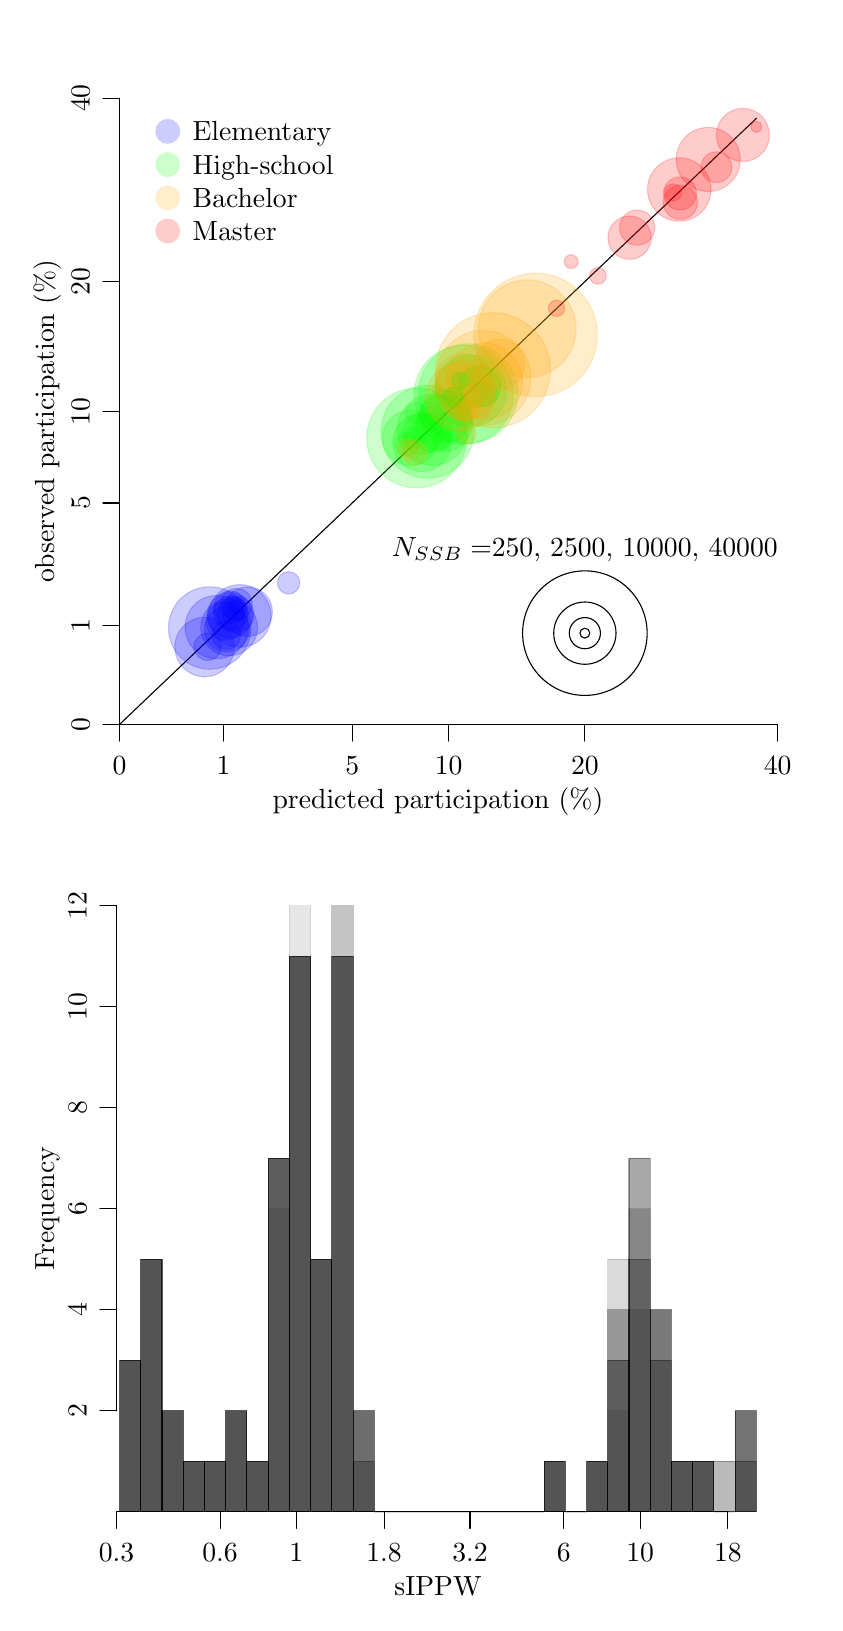
\begin{tikzpicture}[x=1pt,y=1pt]
\definecolor{fillColor}{RGB}{255,255,255}
\path[use as bounding box,fill=fillColor,fill opacity=0.00] (0,0) rectangle (284.53,569.06);
\begin{scope}
\path[clip] (  0.00,284.53) rectangle (284.53,569.06);
\definecolor{drawColor}{RGB}{0,0,0}

\node[text=drawColor,anchor=base,inner sep=0pt, outer sep=0pt, scale=  1.00] at (148.26,286.93) {predicted participation (\%)};

\node[text=drawColor,rotate= 90.00,anchor=base,inner sep=0pt, outer sep=0pt, scale=  1.00] at (  9.60,426.79) {observed participation (\%)};
\end{scope}
\begin{scope}
\path[clip] ( 24.00,308.53) rectangle (272.53,545.06);
\definecolor{drawColor}{RGB}{0,0,0}

\path[draw=drawColor,line width= 0.4pt,line join=round,line cap=round] ( 33.20,317.29) --
	(263.32,536.29);
\definecolor{drawColor}{RGB}{0,0,255}
\definecolor{fillColor}{RGB}{0,0,255}

\path[draw=drawColor,draw opacity=0.20,line width= 0.4pt,line join=round,line cap=round,fill=fillColor,fill opacity=0.20] ( 76.64,356.48) circle ( 11.31);
\definecolor{drawColor}{RGB}{0,255,0}
\definecolor{fillColor}{RGB}{0,255,0}

\path[draw=drawColor,draw opacity=0.20,line width= 0.4pt,line join=round,line cap=round,fill=fillColor,fill opacity=0.20] (165.46,436.52) circle (  4.49);
\definecolor{drawColor}{RGB}{0,0,255}
\definecolor{fillColor}{RGB}{0,0,255}

\path[draw=drawColor,draw opacity=0.20,line width= 0.4pt,line join=round,line cap=round,fill=fillColor,fill opacity=0.20] ( 65.79,352.12) circle ( 14.91);

\path[draw=drawColor,draw opacity=0.20,line width= 0.4pt,line join=round,line cap=round,fill=fillColor,fill opacity=0.20] ( 63.93,345.25) circle ( 10.75);

\path[draw=drawColor,draw opacity=0.20,line width= 0.4pt,line join=round,line cap=round,fill=fillColor,fill opacity=0.20] ( 65.06,345.35) circle (  4.97);
\definecolor{drawColor}{RGB}{0,255,0}
\definecolor{fillColor}{RGB}{0,255,0}

\path[draw=drawColor,draw opacity=0.20,line width= 0.4pt,line join=round,line cap=round,fill=fillColor,fill opacity=0.20] (157.54,436.40) circle ( 17.91);

\path[draw=drawColor,draw opacity=0.20,line width= 0.4pt,line join=round,line cap=round,fill=fillColor,fill opacity=0.20] (142.51,419.20) circle ( 10.54);

\path[draw=drawColor,draw opacity=0.20,line width= 0.4pt,line join=round,line cap=round,fill=fillColor,fill opacity=0.20] (149.54,419.78) circle (  3.27);
\definecolor{drawColor}{RGB}{255,165,0}
\definecolor{fillColor}{RGB}{255,165,0}

\path[draw=drawColor,draw opacity=0.20,line width= 0.4pt,line join=round,line cap=round,fill=fillColor,fill opacity=0.20] (157.37,441.02) circle ( 10.29);

\path[draw=drawColor,draw opacity=0.20,line width= 0.4pt,line join=round,line cap=round,fill=fillColor,fill opacity=0.20] (146.02,427.83) circle (  4.47);
\definecolor{drawColor}{RGB}{0,0,255}
\definecolor{fillColor}{RGB}{0,0,255}

\path[draw=drawColor,draw opacity=0.20,line width= 0.4pt,line join=round,line cap=round,fill=fillColor,fill opacity=0.20] ( 72.79,352.34) circle ( 10.25);

\path[draw=drawColor,draw opacity=0.20,line width= 0.4pt,line join=round,line cap=round,fill=fillColor,fill opacity=0.20] ( 68.30,352.45) circle ( 11.43);

\path[draw=drawColor,draw opacity=0.20,line width= 0.4pt,line join=round,line cap=round,fill=fillColor,fill opacity=0.20] ( 72.00,351.64) circle (  8.16);

\path[draw=drawColor,draw opacity=0.20,line width= 0.4pt,line join=round,line cap=round,fill=fillColor,fill opacity=0.20] ( 71.81,349.49) circle (  5.14);
\definecolor{drawColor}{RGB}{0,255,0}
\definecolor{fillColor}{RGB}{0,255,0}

\path[draw=drawColor,draw opacity=0.20,line width= 0.4pt,line join=round,line cap=round,fill=fillColor,fill opacity=0.20] (159.14,436.87) circle ( 17.97);

\path[draw=drawColor,draw opacity=0.20,line width= 0.4pt,line join=round,line cap=round,fill=fillColor,fill opacity=0.20] (140.55,420.78) circle ( 18.04);

\path[draw=drawColor,draw opacity=0.20,line width= 0.4pt,line join=round,line cap=round,fill=fillColor,fill opacity=0.20] (138.29,420.79) circle ( 10.05);

\path[draw=drawColor,draw opacity=0.20,line width= 0.4pt,line join=round,line cap=round,fill=fillColor,fill opacity=0.20] (137.01,418.51) circle (  4.25);
\definecolor{drawColor}{RGB}{255,165,0}
\definecolor{fillColor}{RGB}{255,165,0}

\path[draw=drawColor,draw opacity=0.20,line width= 0.4pt,line join=round,line cap=round,fill=fillColor,fill opacity=0.20] (183.54,458.02) circle ( 22.31);

\path[draw=drawColor,draw opacity=0.20,line width= 0.4pt,line join=round,line cap=round,fill=fillColor,fill opacity=0.20] (164.63,442.49) circle ( 17.18);

\path[draw=drawColor,draw opacity=0.20,line width= 0.4pt,line join=round,line cap=round,fill=fillColor,fill opacity=0.20] (158.76,439.09) circle (  7.16);

\path[draw=drawColor,draw opacity=0.20,line width= 0.4pt,line join=round,line cap=round,fill=fillColor,fill opacity=0.20] (148.11,438.47) circle (  2.15);
\definecolor{drawColor}{RGB}{255,0,0}
\definecolor{fillColor}{RGB}{255,0,0}

\path[draw=drawColor,draw opacity=0.20,line width= 0.4pt,line join=round,line cap=round,fill=fillColor,fill opacity=0.20] (258.44,530.29) circle (  9.60);

\path[draw=drawColor,draw opacity=0.20,line width= 0.4pt,line join=round,line cap=round,fill=fillColor,fill opacity=0.20] (248.89,518.64) circle (  5.57);
\definecolor{drawColor}{RGB}{0,0,255}
\definecolor{fillColor}{RGB}{0,0,255}

\path[draw=drawColor,draw opacity=0.20,line width= 0.4pt,line join=round,line cap=round,fill=fillColor,fill opacity=0.20] ( 75.15,357.12) circle (  6.61);

\path[draw=drawColor,draw opacity=0.20,line width= 0.4pt,line join=round,line cap=round,fill=fillColor,fill opacity=0.20] ( 79.48,358.01) circle (  8.95);

\path[draw=drawColor,draw opacity=0.20,line width= 0.4pt,line join=round,line cap=round,fill=fillColor,fill opacity=0.20] ( 73.08,356.72) circle (  8.22);

\path[draw=drawColor,draw opacity=0.20,line width= 0.4pt,line join=round,line cap=round,fill=fillColor,fill opacity=0.20] ( 71.38,354.64) circle (  6.92);
\definecolor{drawColor}{RGB}{0,255,0}
\definecolor{fillColor}{RGB}{0,255,0}

\path[draw=drawColor,draw opacity=0.20,line width= 0.4pt,line join=round,line cap=round,fill=fillColor,fill opacity=0.20] (160.11,437.86) circle ( 12.98);

\path[draw=drawColor,draw opacity=0.20,line width= 0.4pt,line join=round,line cap=round,fill=fillColor,fill opacity=0.20] (144.43,423.04) circle ( 16.77);

\path[draw=drawColor,draw opacity=0.20,line width= 0.4pt,line join=round,line cap=round,fill=fillColor,fill opacity=0.20] (146.32,423.69) circle ( 12.77);

\path[draw=drawColor,draw opacity=0.20,line width= 0.4pt,line join=round,line cap=round,fill=fillColor,fill opacity=0.20] (142.51,422.16) circle (  7.29);
\definecolor{drawColor}{RGB}{255,165,0}
\definecolor{fillColor}{RGB}{255,165,0}

\path[draw=drawColor,draw opacity=0.20,line width= 0.4pt,line join=round,line cap=round,fill=fillColor,fill opacity=0.20] (180.52,460.28) circle ( 17.65);

\path[draw=drawColor,draw opacity=0.20,line width= 0.4pt,line join=round,line cap=round,fill=fillColor,fill opacity=0.20] (168.11,445.27) circle ( 20.81);

\path[draw=drawColor,draw opacity=0.20,line width= 0.4pt,line join=round,line cap=round,fill=fillColor,fill opacity=0.20] (165.01,441.22) circle ( 13.85);

\path[draw=drawColor,draw opacity=0.20,line width= 0.4pt,line join=round,line cap=round,fill=fillColor,fill opacity=0.20] (165.39,441.63) circle (  5.75);
\definecolor{drawColor}{RGB}{255,0,0}
\definecolor{fillColor}{RGB}{255,0,0}

\path[draw=drawColor,draw opacity=0.20,line width= 0.4pt,line join=round,line cap=round,fill=fillColor,fill opacity=0.20] (245.92,521.43) circle ( 11.58);

\path[draw=drawColor,draw opacity=0.20,line width= 0.4pt,line join=round,line cap=round,fill=fillColor,fill opacity=0.20] (235.45,510.59) circle ( 11.47);

\path[draw=drawColor,draw opacity=0.20,line width= 0.4pt,line join=round,line cap=round,fill=fillColor,fill opacity=0.20] (235.71,509.15) circle (  5.98);

\path[draw=drawColor,draw opacity=0.20,line width= 0.4pt,line join=round,line cap=round,fill=fillColor,fill opacity=0.20] (263.32,533.20) circle (  2.05);
\definecolor{drawColor}{RGB}{0,0,255}
\definecolor{fillColor}{RGB}{0,0,255}

\path[draw=drawColor,draw opacity=0.20,line width= 0.4pt,line join=round,line cap=round,fill=fillColor,fill opacity=0.20] ( 94.29,368.45) circle (  4.04);

\path[draw=drawColor,draw opacity=0.20,line width= 0.4pt,line join=round,line cap=round,fill=fillColor,fill opacity=0.20] ( 75.38,360.68) circle (  5.76);

\path[draw=drawColor,draw opacity=0.20,line width= 0.4pt,line join=round,line cap=round,fill=fillColor,fill opacity=0.20] ( 73.17,359.61) circle (  5.89);

\path[draw=drawColor,draw opacity=0.20,line width= 0.4pt,line join=round,line cap=round,fill=fillColor,fill opacity=0.20] ( 73.37,357.58) circle (  6.23);
\definecolor{drawColor}{RGB}{0,255,0}
\definecolor{fillColor}{RGB}{0,255,0}

\path[draw=drawColor,draw opacity=0.20,line width= 0.4pt,line join=round,line cap=round,fill=fillColor,fill opacity=0.20] (163.36,439.42) circle (  7.49);

\path[draw=drawColor,draw opacity=0.20,line width= 0.4pt,line join=round,line cap=round,fill=fillColor,fill opacity=0.20] (150.46,426.03) circle ( 10.18);

\path[draw=drawColor,draw opacity=0.20,line width= 0.4pt,line join=round,line cap=round,fill=fillColor,fill opacity=0.20] (151.04,428.52) circle (  9.37);

\path[draw=drawColor,draw opacity=0.20,line width= 0.4pt,line join=round,line cap=round,fill=fillColor,fill opacity=0.20] (146.05,422.94) circle (  7.08);
\definecolor{drawColor}{RGB}{255,165,0}
\definecolor{fillColor}{RGB}{255,165,0}

\path[draw=drawColor,draw opacity=0.20,line width= 0.4pt,line join=round,line cap=round,fill=fillColor,fill opacity=0.20] (170.47,447.33) circle (  9.22);

\path[draw=drawColor,draw opacity=0.20,line width= 0.4pt,line join=round,line cap=round,fill=fillColor,fill opacity=0.20] (156.10,435.50) circle ( 12.29);

\path[draw=drawColor,draw opacity=0.20,line width= 0.4pt,line join=round,line cap=round,fill=fillColor,fill opacity=0.20] (158.29,438.18) circle ( 10.90);

\path[draw=drawColor,draw opacity=0.20,line width= 0.4pt,line join=round,line cap=round,fill=fillColor,fill opacity=0.20] (157.17,433.86) circle (  6.63);
\definecolor{drawColor}{RGB}{255,0,0}
\definecolor{fillColor}{RGB}{255,0,0}

\path[draw=drawColor,draw opacity=0.20,line width= 0.4pt,line join=round,line cap=round,fill=fillColor,fill opacity=0.20] (235.84,505.97) circle (  6.20);

\path[draw=drawColor,draw opacity=0.20,line width= 0.4pt,line join=round,line cap=round,fill=fillColor,fill opacity=0.20] (217.51,493.17) circle (  7.84);

\path[draw=drawColor,draw opacity=0.20,line width= 0.4pt,line join=round,line cap=round,fill=fillColor,fill opacity=0.20] (220.25,496.79) circle (  6.37);

\path[draw=drawColor,draw opacity=0.20,line width= 0.4pt,line join=round,line cap=round,fill=fillColor,fill opacity=0.20] (233.23,509.52) circle (  3.08);
\definecolor{drawColor}{RGB}{0,0,255}
\definecolor{fillColor}{RGB}{0,0,255}

\path[draw=drawColor,draw opacity=0.20,line width= 0.4pt,line join=round,line cap=round,fill=fillColor,fill opacity=0.20] ( 74.92,360.26) circle (  3.04);

\path[draw=drawColor,draw opacity=0.20,line width= 0.4pt,line join=round,line cap=round,fill=fillColor,fill opacity=0.20] ( 75.74,360.28) circle (  2.63);

\path[draw=drawColor,draw opacity=0.20,line width= 0.4pt,line join=round,line cap=round,fill=fillColor,fill opacity=0.20] ( 74.98,358.18) circle (  3.65);
\definecolor{drawColor}{RGB}{0,255,0}
\definecolor{fillColor}{RGB}{0,255,0}

\path[draw=drawColor,draw opacity=0.20,line width= 0.4pt,line join=round,line cap=round,fill=fillColor,fill opacity=0.20] (156.18,441.58) circle (  2.92);

\path[draw=drawColor,draw opacity=0.20,line width= 0.4pt,line join=round,line cap=round,fill=fillColor,fill opacity=0.20] (140.26,429.84) circle (  3.75);

\path[draw=drawColor,draw opacity=0.20,line width= 0.4pt,line join=round,line cap=round,fill=fillColor,fill opacity=0.20] (153.87,435.57) circle (  3.56);

\path[draw=drawColor,draw opacity=0.20,line width= 0.4pt,line join=round,line cap=round,fill=fillColor,fill opacity=0.20] (139.84,420.99) circle (  3.72);
\definecolor{drawColor}{RGB}{255,165,0}
\definecolor{fillColor}{RGB}{255,165,0}

\path[draw=drawColor,draw opacity=0.20,line width= 0.4pt,line join=round,line cap=round,fill=fillColor,fill opacity=0.20] (158.59,422.23) circle (  3.59);

\path[draw=drawColor,draw opacity=0.20,line width= 0.4pt,line join=round,line cap=round,fill=fillColor,fill opacity=0.20] (139.85,415.47) circle (  4.45);

\path[draw=drawColor,draw opacity=0.20,line width= 0.4pt,line join=round,line cap=round,fill=fillColor,fill opacity=0.20] (158.08,430.36) circle (  3.99);

\path[draw=drawColor,draw opacity=0.20,line width= 0.4pt,line join=round,line cap=round,fill=fillColor,fill opacity=0.20] (137.28,416.89) circle (  3.63);
\definecolor{drawColor}{RGB}{255,0,0}
\definecolor{fillColor}{RGB}{255,0,0}

\path[draw=drawColor,draw opacity=0.20,line width= 0.4pt,line join=round,line cap=round,fill=fillColor,fill opacity=0.20] (196.38,484.52) circle (  2.51);

\path[draw=drawColor,draw opacity=0.20,line width= 0.4pt,line join=round,line cap=round,fill=fillColor,fill opacity=0.20] (191.11,467.64) circle (  2.95);

\path[draw=drawColor,draw opacity=0.20,line width= 0.4pt,line join=round,line cap=round,fill=fillColor,fill opacity=0.20] (206.04,479.39) circle (  3.03);
\end{scope}
\begin{scope}
\path[clip] (  0.00,  0.00) rectangle (284.53,569.06);
\definecolor{drawColor}{RGB}{0,0,0}

\path[draw=drawColor,line width= 0.4pt,line join=round,line cap=round] ( 33.20,317.29) -- (270.99,317.29);

\path[draw=drawColor,line width= 0.4pt,line join=round,line cap=round] ( 33.20,317.29) -- ( 33.20,311.29);

\path[draw=drawColor,line width= 0.4pt,line join=round,line cap=round] ( 70.80,317.29) -- ( 70.80,311.29);

\path[draw=drawColor,line width= 0.4pt,line join=round,line cap=round] (117.27,317.29) -- (117.27,311.29);

\path[draw=drawColor,line width= 0.4pt,line join=round,line cap=round] (152.10,317.29) -- (152.10,311.29);

\path[draw=drawColor,line width= 0.4pt,line join=round,line cap=round] (201.34,317.29) -- (201.34,311.29);

\path[draw=drawColor,line width= 0.4pt,line join=round,line cap=round] (270.99,317.29) -- (270.99,311.29);

\node[text=drawColor,anchor=base,inner sep=0pt, outer sep=0pt, scale=  1.00] at ( 33.20,299.29) {0};

\node[text=drawColor,anchor=base,inner sep=0pt, outer sep=0pt, scale=  1.00] at ( 70.80,299.29) {1};

\node[text=drawColor,anchor=base,inner sep=0pt, outer sep=0pt, scale=  1.00] at (117.27,299.29) {5};

\node[text=drawColor,anchor=base,inner sep=0pt, outer sep=0pt, scale=  1.00] at (152.10,299.29) {10};

\node[text=drawColor,anchor=base,inner sep=0pt, outer sep=0pt, scale=  1.00] at (201.34,299.29) {20};

\node[text=drawColor,anchor=base,inner sep=0pt, outer sep=0pt, scale=  1.00] at (270.99,299.29) {40};

\path[draw=drawColor,line width= 0.4pt,line join=round,line cap=round] ( 33.20,317.29) -- ( 33.20,543.59);

\path[draw=drawColor,line width= 0.4pt,line join=round,line cap=round] ( 33.20,317.29) -- ( 27.20,317.29);

\path[draw=drawColor,line width= 0.4pt,line join=round,line cap=round] ( 33.20,353.07) -- ( 27.20,353.07);

\path[draw=drawColor,line width= 0.4pt,line join=round,line cap=round] ( 33.20,397.30) -- ( 27.20,397.30);

\path[draw=drawColor,line width= 0.4pt,line join=round,line cap=round] ( 33.20,430.44) -- ( 27.20,430.44);

\path[draw=drawColor,line width= 0.4pt,line join=round,line cap=round] ( 33.20,477.31) -- ( 27.20,477.31);

\path[draw=drawColor,line width= 0.4pt,line join=round,line cap=round] ( 33.20,543.59) -- ( 27.20,543.59);

\node[text=drawColor,rotate= 90.00,anchor=base,inner sep=0pt, outer sep=0pt, scale=  1.00] at ( 22.40,317.29) {0};

\node[text=drawColor,rotate= 90.00,anchor=base,inner sep=0pt, outer sep=0pt, scale=  1.00] at ( 22.40,353.07) {1};

\node[text=drawColor,rotate= 90.00,anchor=base,inner sep=0pt, outer sep=0pt, scale=  1.00] at ( 22.40,397.30) {5};

\node[text=drawColor,rotate= 90.00,anchor=base,inner sep=0pt, outer sep=0pt, scale=  1.00] at ( 22.40,430.44) {10};

\node[text=drawColor,rotate= 90.00,anchor=base,inner sep=0pt, outer sep=0pt, scale=  1.00] at ( 22.40,477.31) {20};

\node[text=drawColor,rotate= 90.00,anchor=base,inner sep=0pt, outer sep=0pt, scale=  1.00] at ( 22.40,543.59) {40};
\end{scope}
\begin{scope}
\path[clip] ( 24.00,308.53) rectangle (272.53,545.06);
\definecolor{drawColor}{RGB}{0,0,0}

\path[draw=drawColor,line width= 0.4pt,line join=round,line cap=round] (201.34,350.27) circle (  1.78);

\path[draw=drawColor,line width= 0.4pt,line join=round,line cap=round] (201.34,350.27) circle (  5.63);

\path[draw=drawColor,line width= 0.4pt,line join=round,line cap=round] (201.34,350.27) circle ( 11.25);

\path[draw=drawColor,line width= 0.4pt,line join=round,line cap=round] (201.34,350.27) circle ( 22.50);

\node[text=drawColor,anchor=base,inner sep=0pt, outer sep=0pt, scale=  1.00] at (201.34,377.94) {$N_{SSB}=$250, 2500, 10000, 40000};
\definecolor{fillColor}{RGB}{0,0,255}

\path[fill=fillColor,fill opacity=0.20] ( 50.61,531.59) circle (  4.50);
\definecolor{fillColor}{RGB}{0,255,0}

\path[fill=fillColor,fill opacity=0.20] ( 50.61,519.59) circle (  4.50);
\definecolor{fillColor}{RGB}{255,165,0}

\path[fill=fillColor,fill opacity=0.20] ( 50.61,507.59) circle (  4.50);
\definecolor{fillColor}{RGB}{255,0,0}

\path[fill=fillColor,fill opacity=0.20] ( 50.61,495.59) circle (  4.50);

\node[text=drawColor,anchor=base west,inner sep=0pt, outer sep=0pt, scale=  1.00] at ( 59.61,528.15) {Elementary};

\node[text=drawColor,anchor=base west,inner sep=0pt, outer sep=0pt, scale=  1.00] at ( 59.61,516.15) {High-school};

\node[text=drawColor,anchor=base west,inner sep=0pt, outer sep=0pt, scale=  1.00] at ( 59.61,504.15) {Bachelor};

\node[text=drawColor,anchor=base west,inner sep=0pt, outer sep=0pt, scale=  1.00] at ( 59.61,492.15) {Master};
\end{scope}
\begin{scope}
\path[clip] (  0.00,  0.00) rectangle (284.53,284.53);
\definecolor{drawColor}{RGB}{0,0,0}

\node[text=drawColor,anchor=base,inner sep=0pt, outer sep=0pt, scale=  1.00] at (148.26,  2.40) {sIPPW};

\node[text=drawColor,rotate= 90.00,anchor=base,inner sep=0pt, outer sep=0pt, scale=  1.00] at (  9.60,142.26) {Frequency};
\end{scope}
\begin{scope}
\path[clip] ( 24.00, 24.00) rectangle (272.53,260.53);
\definecolor{drawColor}{RGB}{0,0,0}
\definecolor{fillColor}{RGB}{0,0,0}

\path[draw=drawColor,draw opacity=0.05,line width= 0.4pt,line join=round,line cap=round,fill=fillColor,fill opacity=0.10] ( 33.20, 32.76) rectangle ( 40.88, 87.51);

\path[draw=drawColor,draw opacity=0.05,line width= 0.4pt,line join=round,line cap=round,fill=fillColor,fill opacity=0.10] ( 40.88, 32.76) rectangle ( 48.55,124.01);

\path[draw=drawColor,draw opacity=0.05,line width= 0.4pt,line join=round,line cap=round,fill=fillColor,fill opacity=0.10] ( 48.55, 32.76) rectangle ( 56.22, 69.26);

\path[draw=drawColor,draw opacity=0.05,line width= 0.4pt,line join=round,line cap=round,fill=fillColor,fill opacity=0.10] ( 56.22, 32.76) rectangle ( 63.89, 51.01);

\path[draw=drawColor,draw opacity=0.05,line width= 0.4pt,line join=round,line cap=round,fill=fillColor,fill opacity=0.10] ( 63.89, 32.76) rectangle ( 71.56, 51.01);

\path[draw=drawColor,draw opacity=0.05,line width= 0.4pt,line join=round,line cap=round,fill=fillColor,fill opacity=0.10] ( 71.56, 32.76) rectangle ( 79.23, 69.26);

\path[draw=drawColor,draw opacity=0.05,line width= 0.4pt,line join=round,line cap=round,fill=fillColor,fill opacity=0.10] ( 79.23, 32.76) rectangle ( 86.90, 51.01);

\path[draw=drawColor,draw opacity=0.05,line width= 0.4pt,line join=round,line cap=round,fill=fillColor,fill opacity=0.10] ( 86.90, 32.76) rectangle ( 94.57,160.51);

\path[draw=drawColor,draw opacity=0.05,line width= 0.4pt,line join=round,line cap=round,fill=fillColor,fill opacity=0.10] ( 94.57, 32.76) rectangle (102.24,233.52);

\path[draw=drawColor,draw opacity=0.05,line width= 0.4pt,line join=round,line cap=round,fill=fillColor,fill opacity=0.10] (102.24, 32.76) rectangle (109.91,124.01);

\path[draw=drawColor,draw opacity=0.05,line width= 0.4pt,line join=round,line cap=round,fill=fillColor,fill opacity=0.10] (109.91, 32.76) rectangle (117.58,233.52);

\path[draw=drawColor,draw opacity=0.05,line width= 0.4pt,line join=round,line cap=round,fill=fillColor,fill opacity=0.10] (117.58, 32.76) rectangle (125.25, 69.26);

\path[draw=drawColor,draw opacity=0.05,line width= 0.4pt,line join=round,line cap=round,fill=fillColor,fill opacity=0.10] (125.25, 32.76) rectangle (132.92, 32.76);

\path[draw=drawColor,draw opacity=0.05,line width= 0.4pt,line join=round,line cap=round,fill=fillColor,fill opacity=0.10] (132.92, 32.76) rectangle (140.59, 32.76);

\path[draw=drawColor,draw opacity=0.05,line width= 0.4pt,line join=round,line cap=round,fill=fillColor,fill opacity=0.10] (140.59, 32.76) rectangle (148.26, 32.76);

\path[draw=drawColor,draw opacity=0.05,line width= 0.4pt,line join=round,line cap=round,fill=fillColor,fill opacity=0.10] (148.26, 32.76) rectangle (155.93, 32.76);

\path[draw=drawColor,draw opacity=0.05,line width= 0.4pt,line join=round,line cap=round,fill=fillColor,fill opacity=0.10] (155.93, 32.76) rectangle (163.60, 32.76);

\path[draw=drawColor,draw opacity=0.05,line width= 0.4pt,line join=round,line cap=round,fill=fillColor,fill opacity=0.10] (163.60, 32.76) rectangle (171.28, 32.76);

\path[draw=drawColor,draw opacity=0.05,line width= 0.4pt,line join=round,line cap=round,fill=fillColor,fill opacity=0.10] (171.28, 32.76) rectangle (178.95, 32.76);

\path[draw=drawColor,draw opacity=0.05,line width= 0.4pt,line join=round,line cap=round,fill=fillColor,fill opacity=0.10] (178.95, 32.76) rectangle (186.62, 32.76);

\path[draw=drawColor,draw opacity=0.05,line width= 0.4pt,line join=round,line cap=round,fill=fillColor,fill opacity=0.10] (186.62, 32.76) rectangle (194.29, 51.01);

\path[draw=drawColor,draw opacity=0.05,line width= 0.4pt,line join=round,line cap=round,fill=fillColor,fill opacity=0.10] (194.29, 32.76) rectangle (201.96, 32.76);

\path[draw=drawColor,draw opacity=0.05,line width= 0.4pt,line join=round,line cap=round,fill=fillColor,fill opacity=0.10] (201.96, 32.76) rectangle (209.63, 51.01);

\path[draw=drawColor,draw opacity=0.05,line width= 0.4pt,line join=round,line cap=round,fill=fillColor,fill opacity=0.10] (209.63, 32.76) rectangle (217.30, 87.51);

\path[draw=drawColor,draw opacity=0.05,line width= 0.4pt,line join=round,line cap=round,fill=fillColor,fill opacity=0.10] (217.30, 32.76) rectangle (224.97,142.26);

\path[draw=drawColor,draw opacity=0.05,line width= 0.4pt,line join=round,line cap=round,fill=fillColor,fill opacity=0.10] (224.97, 32.76) rectangle (232.64,105.76);

\path[draw=drawColor,draw opacity=0.05,line width= 0.4pt,line join=round,line cap=round,fill=fillColor,fill opacity=0.10] (232.64, 32.76) rectangle (240.31, 51.01);

\path[draw=drawColor,draw opacity=0.05,line width= 0.4pt,line join=round,line cap=round,fill=fillColor,fill opacity=0.10] (240.31, 32.76) rectangle (247.98, 51.01);

\path[draw=drawColor,draw opacity=0.05,line width= 0.4pt,line join=round,line cap=round,fill=fillColor,fill opacity=0.10] (247.98, 32.76) rectangle (255.65, 32.76);

\path[draw=drawColor,draw opacity=0.05,line width= 0.4pt,line join=round,line cap=round,fill=fillColor,fill opacity=0.10] (255.65, 32.76) rectangle (263.32, 69.26);
\definecolor{fillColor}{RGB}{0,0,0}

\path[draw=drawColor,draw opacity=0.05,line width= 0.4pt,line join=round,line cap=round,fill=fillColor,fill opacity=0.05] ( 33.20, 32.76) rectangle ( 40.88, 87.51);

\path[draw=drawColor,draw opacity=0.05,line width= 0.4pt,line join=round,line cap=round,fill=fillColor,fill opacity=0.05] ( 40.88, 32.76) rectangle ( 48.55,124.01);

\path[draw=drawColor,draw opacity=0.05,line width= 0.4pt,line join=round,line cap=round,fill=fillColor,fill opacity=0.05] ( 48.55, 32.76) rectangle ( 56.22, 69.26);

\path[draw=drawColor,draw opacity=0.05,line width= 0.4pt,line join=round,line cap=round,fill=fillColor,fill opacity=0.05] ( 56.22, 32.76) rectangle ( 63.89, 51.01);

\path[draw=drawColor,draw opacity=0.05,line width= 0.4pt,line join=round,line cap=round,fill=fillColor,fill opacity=0.05] ( 63.89, 32.76) rectangle ( 71.56, 51.01);

\path[draw=drawColor,draw opacity=0.05,line width= 0.4pt,line join=round,line cap=round,fill=fillColor,fill opacity=0.05] ( 71.56, 32.76) rectangle ( 79.23, 69.26);

\path[draw=drawColor,draw opacity=0.05,line width= 0.4pt,line join=round,line cap=round,fill=fillColor,fill opacity=0.05] ( 79.23, 32.76) rectangle ( 86.90, 51.01);

\path[draw=drawColor,draw opacity=0.05,line width= 0.4pt,line join=round,line cap=round,fill=fillColor,fill opacity=0.05] ( 86.90, 32.76) rectangle ( 94.57,160.51);

\path[draw=drawColor,draw opacity=0.05,line width= 0.4pt,line join=round,line cap=round,fill=fillColor,fill opacity=0.05] ( 94.57, 32.76) rectangle (102.24,233.52);

\path[draw=drawColor,draw opacity=0.05,line width= 0.4pt,line join=round,line cap=round,fill=fillColor,fill opacity=0.05] (102.24, 32.76) rectangle (109.91,124.01);

\path[draw=drawColor,draw opacity=0.05,line width= 0.4pt,line join=round,line cap=round,fill=fillColor,fill opacity=0.05] (109.91, 32.76) rectangle (117.58,251.77);

\path[draw=drawColor,draw opacity=0.05,line width= 0.4pt,line join=round,line cap=round,fill=fillColor,fill opacity=0.05] (117.58, 32.76) rectangle (125.25, 51.01);

\path[draw=drawColor,draw opacity=0.05,line width= 0.4pt,line join=round,line cap=round,fill=fillColor,fill opacity=0.05] (125.25, 32.76) rectangle (132.92, 32.76);

\path[draw=drawColor,draw opacity=0.05,line width= 0.4pt,line join=round,line cap=round,fill=fillColor,fill opacity=0.05] (132.92, 32.76) rectangle (140.59, 32.76);

\path[draw=drawColor,draw opacity=0.05,line width= 0.4pt,line join=round,line cap=round,fill=fillColor,fill opacity=0.05] (140.59, 32.76) rectangle (148.26, 32.76);

\path[draw=drawColor,draw opacity=0.05,line width= 0.4pt,line join=round,line cap=round,fill=fillColor,fill opacity=0.05] (148.26, 32.76) rectangle (155.93, 32.76);

\path[draw=drawColor,draw opacity=0.05,line width= 0.4pt,line join=round,line cap=round,fill=fillColor,fill opacity=0.05] (155.93, 32.76) rectangle (163.60, 32.76);

\path[draw=drawColor,draw opacity=0.05,line width= 0.4pt,line join=round,line cap=round,fill=fillColor,fill opacity=0.05] (163.60, 32.76) rectangle (171.28, 32.76);

\path[draw=drawColor,draw opacity=0.05,line width= 0.4pt,line join=round,line cap=round,fill=fillColor,fill opacity=0.05] (171.28, 32.76) rectangle (178.95, 32.76);

\path[draw=drawColor,draw opacity=0.05,line width= 0.4pt,line join=round,line cap=round,fill=fillColor,fill opacity=0.05] (178.95, 32.76) rectangle (186.62, 32.76);

\path[draw=drawColor,draw opacity=0.05,line width= 0.4pt,line join=round,line cap=round,fill=fillColor,fill opacity=0.05] (186.62, 32.76) rectangle (194.29, 51.01);

\path[draw=drawColor,draw opacity=0.05,line width= 0.4pt,line join=round,line cap=round,fill=fillColor,fill opacity=0.05] (194.29, 32.76) rectangle (201.96, 32.76);

\path[draw=drawColor,draw opacity=0.05,line width= 0.4pt,line join=round,line cap=round,fill=fillColor,fill opacity=0.05] (201.96, 32.76) rectangle (209.63, 51.01);

\path[draw=drawColor,draw opacity=0.05,line width= 0.4pt,line join=round,line cap=round,fill=fillColor,fill opacity=0.05] (209.63, 32.76) rectangle (217.30, 87.51);

\path[draw=drawColor,draw opacity=0.05,line width= 0.4pt,line join=round,line cap=round,fill=fillColor,fill opacity=0.05] (217.30, 32.76) rectangle (224.97,160.51);

\path[draw=drawColor,draw opacity=0.05,line width= 0.4pt,line join=round,line cap=round,fill=fillColor,fill opacity=0.05] (224.97, 32.76) rectangle (232.64, 87.51);

\path[draw=drawColor,draw opacity=0.05,line width= 0.4pt,line join=round,line cap=round,fill=fillColor,fill opacity=0.05] (232.64, 32.76) rectangle (240.31, 51.01);

\path[draw=drawColor,draw opacity=0.05,line width= 0.4pt,line join=round,line cap=round,fill=fillColor,fill opacity=0.05] (240.31, 32.76) rectangle (247.98, 51.01);

\path[draw=drawColor,draw opacity=0.05,line width= 0.4pt,line join=round,line cap=round,fill=fillColor,fill opacity=0.05] (247.98, 32.76) rectangle (255.65, 32.76);

\path[draw=drawColor,draw opacity=0.05,line width= 0.4pt,line join=round,line cap=round,fill=fillColor,fill opacity=0.05] (255.65, 32.76) rectangle (263.32, 69.26);

\path[draw=drawColor,draw opacity=0.05,line width= 0.4pt,line join=round,line cap=round,fill=fillColor,fill opacity=0.05] ( 33.20, 32.76) rectangle ( 40.88, 87.51);

\path[draw=drawColor,draw opacity=0.05,line width= 0.4pt,line join=round,line cap=round,fill=fillColor,fill opacity=0.05] ( 40.88, 32.76) rectangle ( 48.55,124.01);

\path[draw=drawColor,draw opacity=0.05,line width= 0.4pt,line join=round,line cap=round,fill=fillColor,fill opacity=0.05] ( 48.55, 32.76) rectangle ( 56.22, 69.26);

\path[draw=drawColor,draw opacity=0.05,line width= 0.4pt,line join=round,line cap=round,fill=fillColor,fill opacity=0.05] ( 56.22, 32.76) rectangle ( 63.89, 51.01);

\path[draw=drawColor,draw opacity=0.05,line width= 0.4pt,line join=round,line cap=round,fill=fillColor,fill opacity=0.05] ( 63.89, 32.76) rectangle ( 71.56, 51.01);

\path[draw=drawColor,draw opacity=0.05,line width= 0.4pt,line join=round,line cap=round,fill=fillColor,fill opacity=0.05] ( 71.56, 32.76) rectangle ( 79.23, 69.26);

\path[draw=drawColor,draw opacity=0.05,line width= 0.4pt,line join=round,line cap=round,fill=fillColor,fill opacity=0.05] ( 79.23, 32.76) rectangle ( 86.90, 51.01);

\path[draw=drawColor,draw opacity=0.05,line width= 0.4pt,line join=round,line cap=round,fill=fillColor,fill opacity=0.05] ( 86.90, 32.76) rectangle ( 94.57,142.26);

\path[draw=drawColor,draw opacity=0.05,line width= 0.4pt,line join=round,line cap=round,fill=fillColor,fill opacity=0.05] ( 94.57, 32.76) rectangle (102.24,251.77);

\path[draw=drawColor,draw opacity=0.05,line width= 0.4pt,line join=round,line cap=round,fill=fillColor,fill opacity=0.05] (102.24, 32.76) rectangle (109.91,124.01);

\path[draw=drawColor,draw opacity=0.05,line width= 0.4pt,line join=round,line cap=round,fill=fillColor,fill opacity=0.05] (109.91, 32.76) rectangle (117.58,233.52);

\path[draw=drawColor,draw opacity=0.05,line width= 0.4pt,line join=round,line cap=round,fill=fillColor,fill opacity=0.05] (117.58, 32.76) rectangle (125.25, 69.26);

\path[draw=drawColor,draw opacity=0.05,line width= 0.4pt,line join=round,line cap=round,fill=fillColor,fill opacity=0.05] (125.25, 32.76) rectangle (132.92, 32.76);

\path[draw=drawColor,draw opacity=0.05,line width= 0.4pt,line join=round,line cap=round,fill=fillColor,fill opacity=0.05] (132.92, 32.76) rectangle (140.59, 32.76);

\path[draw=drawColor,draw opacity=0.05,line width= 0.4pt,line join=round,line cap=round,fill=fillColor,fill opacity=0.05] (140.59, 32.76) rectangle (148.26, 32.76);

\path[draw=drawColor,draw opacity=0.05,line width= 0.4pt,line join=round,line cap=round,fill=fillColor,fill opacity=0.05] (148.26, 32.76) rectangle (155.93, 32.76);

\path[draw=drawColor,draw opacity=0.05,line width= 0.4pt,line join=round,line cap=round,fill=fillColor,fill opacity=0.05] (155.93, 32.76) rectangle (163.60, 32.76);

\path[draw=drawColor,draw opacity=0.05,line width= 0.4pt,line join=round,line cap=round,fill=fillColor,fill opacity=0.05] (163.60, 32.76) rectangle (171.28, 32.76);

\path[draw=drawColor,draw opacity=0.05,line width= 0.4pt,line join=round,line cap=round,fill=fillColor,fill opacity=0.05] (171.28, 32.76) rectangle (178.95, 32.76);

\path[draw=drawColor,draw opacity=0.05,line width= 0.4pt,line join=round,line cap=round,fill=fillColor,fill opacity=0.05] (178.95, 32.76) rectangle (186.62, 32.76);

\path[draw=drawColor,draw opacity=0.05,line width= 0.4pt,line join=round,line cap=round,fill=fillColor,fill opacity=0.05] (186.62, 32.76) rectangle (194.29, 51.01);

\path[draw=drawColor,draw opacity=0.05,line width= 0.4pt,line join=round,line cap=round,fill=fillColor,fill opacity=0.05] (194.29, 32.76) rectangle (201.96, 32.76);

\path[draw=drawColor,draw opacity=0.05,line width= 0.4pt,line join=round,line cap=round,fill=fillColor,fill opacity=0.05] (201.96, 32.76) rectangle (209.63, 51.01);

\path[draw=drawColor,draw opacity=0.05,line width= 0.4pt,line join=round,line cap=round,fill=fillColor,fill opacity=0.05] (209.63, 32.76) rectangle (217.30,105.76);

\path[draw=drawColor,draw opacity=0.05,line width= 0.4pt,line join=round,line cap=round,fill=fillColor,fill opacity=0.05] (217.30, 32.76) rectangle (224.97,124.01);

\path[draw=drawColor,draw opacity=0.05,line width= 0.4pt,line join=round,line cap=round,fill=fillColor,fill opacity=0.05] (224.97, 32.76) rectangle (232.64,105.76);

\path[draw=drawColor,draw opacity=0.05,line width= 0.4pt,line join=round,line cap=round,fill=fillColor,fill opacity=0.05] (232.64, 32.76) rectangle (240.31, 51.01);

\path[draw=drawColor,draw opacity=0.05,line width= 0.4pt,line join=round,line cap=round,fill=fillColor,fill opacity=0.05] (240.31, 32.76) rectangle (247.98, 51.01);

\path[draw=drawColor,draw opacity=0.05,line width= 0.4pt,line join=round,line cap=round,fill=fillColor,fill opacity=0.05] (247.98, 32.76) rectangle (255.65, 51.01);

\path[draw=drawColor,draw opacity=0.05,line width= 0.4pt,line join=round,line cap=round,fill=fillColor,fill opacity=0.05] (255.65, 32.76) rectangle (263.32, 51.01);

\path[draw=drawColor,draw opacity=0.05,line width= 0.4pt,line join=round,line cap=round,fill=fillColor,fill opacity=0.05] ( 33.20, 32.76) rectangle ( 40.88, 87.51);

\path[draw=drawColor,draw opacity=0.05,line width= 0.4pt,line join=round,line cap=round,fill=fillColor,fill opacity=0.05] ( 40.88, 32.76) rectangle ( 48.55,124.01);

\path[draw=drawColor,draw opacity=0.05,line width= 0.4pt,line join=round,line cap=round,fill=fillColor,fill opacity=0.05] ( 48.55, 32.76) rectangle ( 56.22, 69.26);

\path[draw=drawColor,draw opacity=0.05,line width= 0.4pt,line join=round,line cap=round,fill=fillColor,fill opacity=0.05] ( 56.22, 32.76) rectangle ( 63.89, 51.01);

\path[draw=drawColor,draw opacity=0.05,line width= 0.4pt,line join=round,line cap=round,fill=fillColor,fill opacity=0.05] ( 63.89, 32.76) rectangle ( 71.56, 51.01);

\path[draw=drawColor,draw opacity=0.05,line width= 0.4pt,line join=round,line cap=round,fill=fillColor,fill opacity=0.05] ( 71.56, 32.76) rectangle ( 79.23, 69.26);

\path[draw=drawColor,draw opacity=0.05,line width= 0.4pt,line join=round,line cap=round,fill=fillColor,fill opacity=0.05] ( 79.23, 32.76) rectangle ( 86.90, 51.01);

\path[draw=drawColor,draw opacity=0.05,line width= 0.4pt,line join=round,line cap=round,fill=fillColor,fill opacity=0.05] ( 86.90, 32.76) rectangle ( 94.57,160.51);

\path[draw=drawColor,draw opacity=0.05,line width= 0.4pt,line join=round,line cap=round,fill=fillColor,fill opacity=0.05] ( 94.57, 32.76) rectangle (102.24,233.52);

\path[draw=drawColor,draw opacity=0.05,line width= 0.4pt,line join=round,line cap=round,fill=fillColor,fill opacity=0.05] (102.24, 32.76) rectangle (109.91,124.01);

\path[draw=drawColor,draw opacity=0.05,line width= 0.4pt,line join=round,line cap=round,fill=fillColor,fill opacity=0.05] (109.91, 32.76) rectangle (117.58,251.77);

\path[draw=drawColor,draw opacity=0.05,line width= 0.4pt,line join=round,line cap=round,fill=fillColor,fill opacity=0.05] (117.58, 32.76) rectangle (125.25, 51.01);

\path[draw=drawColor,draw opacity=0.05,line width= 0.4pt,line join=round,line cap=round,fill=fillColor,fill opacity=0.05] (125.25, 32.76) rectangle (132.92, 32.76);

\path[draw=drawColor,draw opacity=0.05,line width= 0.4pt,line join=round,line cap=round,fill=fillColor,fill opacity=0.05] (132.92, 32.76) rectangle (140.59, 32.76);

\path[draw=drawColor,draw opacity=0.05,line width= 0.4pt,line join=round,line cap=round,fill=fillColor,fill opacity=0.05] (140.59, 32.76) rectangle (148.26, 32.76);

\path[draw=drawColor,draw opacity=0.05,line width= 0.4pt,line join=round,line cap=round,fill=fillColor,fill opacity=0.05] (148.26, 32.76) rectangle (155.93, 32.76);

\path[draw=drawColor,draw opacity=0.05,line width= 0.4pt,line join=round,line cap=round,fill=fillColor,fill opacity=0.05] (155.93, 32.76) rectangle (163.60, 32.76);

\path[draw=drawColor,draw opacity=0.05,line width= 0.4pt,line join=round,line cap=round,fill=fillColor,fill opacity=0.05] (163.60, 32.76) rectangle (171.28, 32.76);

\path[draw=drawColor,draw opacity=0.05,line width= 0.4pt,line join=round,line cap=round,fill=fillColor,fill opacity=0.05] (171.28, 32.76) rectangle (178.95, 32.76);

\path[draw=drawColor,draw opacity=0.05,line width= 0.4pt,line join=round,line cap=round,fill=fillColor,fill opacity=0.05] (178.95, 32.76) rectangle (186.62, 32.76);

\path[draw=drawColor,draw opacity=0.05,line width= 0.4pt,line join=round,line cap=round,fill=fillColor,fill opacity=0.05] (186.62, 32.76) rectangle (194.29, 51.01);

\path[draw=drawColor,draw opacity=0.05,line width= 0.4pt,line join=round,line cap=round,fill=fillColor,fill opacity=0.05] (194.29, 32.76) rectangle (201.96, 32.76);

\path[draw=drawColor,draw opacity=0.05,line width= 0.4pt,line join=round,line cap=round,fill=fillColor,fill opacity=0.05] (201.96, 32.76) rectangle (209.63, 51.01);

\path[draw=drawColor,draw opacity=0.05,line width= 0.4pt,line join=round,line cap=round,fill=fillColor,fill opacity=0.05] (209.63, 32.76) rectangle (217.30,105.76);

\path[draw=drawColor,draw opacity=0.05,line width= 0.4pt,line join=round,line cap=round,fill=fillColor,fill opacity=0.05] (217.30, 32.76) rectangle (224.97,142.26);

\path[draw=drawColor,draw opacity=0.05,line width= 0.4pt,line join=round,line cap=round,fill=fillColor,fill opacity=0.05] (224.97, 32.76) rectangle (232.64, 87.51);

\path[draw=drawColor,draw opacity=0.05,line width= 0.4pt,line join=round,line cap=round,fill=fillColor,fill opacity=0.05] (232.64, 32.76) rectangle (240.31, 51.01);

\path[draw=drawColor,draw opacity=0.05,line width= 0.4pt,line join=round,line cap=round,fill=fillColor,fill opacity=0.05] (240.31, 32.76) rectangle (247.98, 51.01);

\path[draw=drawColor,draw opacity=0.05,line width= 0.4pt,line join=round,line cap=round,fill=fillColor,fill opacity=0.05] (247.98, 32.76) rectangle (255.65, 51.01);

\path[draw=drawColor,draw opacity=0.05,line width= 0.4pt,line join=round,line cap=round,fill=fillColor,fill opacity=0.05] (255.65, 32.76) rectangle (263.32, 51.01);

\path[draw=drawColor,draw opacity=0.05,line width= 0.4pt,line join=round,line cap=round,fill=fillColor,fill opacity=0.05] ( 33.20, 32.76) rectangle ( 40.88, 87.51);

\path[draw=drawColor,draw opacity=0.05,line width= 0.4pt,line join=round,line cap=round,fill=fillColor,fill opacity=0.05] ( 40.88, 32.76) rectangle ( 48.55,124.01);

\path[draw=drawColor,draw opacity=0.05,line width= 0.4pt,line join=round,line cap=round,fill=fillColor,fill opacity=0.05] ( 48.55, 32.76) rectangle ( 56.22, 69.26);

\path[draw=drawColor,draw opacity=0.05,line width= 0.4pt,line join=round,line cap=round,fill=fillColor,fill opacity=0.05] ( 56.22, 32.76) rectangle ( 63.89, 51.01);

\path[draw=drawColor,draw opacity=0.05,line width= 0.4pt,line join=round,line cap=round,fill=fillColor,fill opacity=0.05] ( 63.89, 32.76) rectangle ( 71.56, 51.01);

\path[draw=drawColor,draw opacity=0.05,line width= 0.4pt,line join=round,line cap=round,fill=fillColor,fill opacity=0.05] ( 71.56, 32.76) rectangle ( 79.23, 69.26);

\path[draw=drawColor,draw opacity=0.05,line width= 0.4pt,line join=round,line cap=round,fill=fillColor,fill opacity=0.05] ( 79.23, 32.76) rectangle ( 86.90, 51.01);

\path[draw=drawColor,draw opacity=0.05,line width= 0.4pt,line join=round,line cap=round,fill=fillColor,fill opacity=0.05] ( 86.90, 32.76) rectangle ( 94.57,160.51);

\path[draw=drawColor,draw opacity=0.05,line width= 0.4pt,line join=round,line cap=round,fill=fillColor,fill opacity=0.05] ( 94.57, 32.76) rectangle (102.24,233.52);

\path[draw=drawColor,draw opacity=0.05,line width= 0.4pt,line join=round,line cap=round,fill=fillColor,fill opacity=0.05] (102.24, 32.76) rectangle (109.91,124.01);

\path[draw=drawColor,draw opacity=0.05,line width= 0.4pt,line join=round,line cap=round,fill=fillColor,fill opacity=0.05] (109.91, 32.76) rectangle (117.58,233.52);

\path[draw=drawColor,draw opacity=0.05,line width= 0.4pt,line join=round,line cap=round,fill=fillColor,fill opacity=0.05] (117.58, 32.76) rectangle (125.25, 69.26);

\path[draw=drawColor,draw opacity=0.05,line width= 0.4pt,line join=round,line cap=round,fill=fillColor,fill opacity=0.05] (125.25, 32.76) rectangle (132.92, 32.76);

\path[draw=drawColor,draw opacity=0.05,line width= 0.4pt,line join=round,line cap=round,fill=fillColor,fill opacity=0.05] (132.92, 32.76) rectangle (140.59, 32.76);

\path[draw=drawColor,draw opacity=0.05,line width= 0.4pt,line join=round,line cap=round,fill=fillColor,fill opacity=0.05] (140.59, 32.76) rectangle (148.26, 32.76);

\path[draw=drawColor,draw opacity=0.05,line width= 0.4pt,line join=round,line cap=round,fill=fillColor,fill opacity=0.05] (148.26, 32.76) rectangle (155.93, 32.76);

\path[draw=drawColor,draw opacity=0.05,line width= 0.4pt,line join=round,line cap=round,fill=fillColor,fill opacity=0.05] (155.93, 32.76) rectangle (163.60, 32.76);

\path[draw=drawColor,draw opacity=0.05,line width= 0.4pt,line join=round,line cap=round,fill=fillColor,fill opacity=0.05] (163.60, 32.76) rectangle (171.28, 32.76);

\path[draw=drawColor,draw opacity=0.05,line width= 0.4pt,line join=round,line cap=round,fill=fillColor,fill opacity=0.05] (171.28, 32.76) rectangle (178.95, 32.76);

\path[draw=drawColor,draw opacity=0.05,line width= 0.4pt,line join=round,line cap=round,fill=fillColor,fill opacity=0.05] (178.95, 32.76) rectangle (186.62, 32.76);

\path[draw=drawColor,draw opacity=0.05,line width= 0.4pt,line join=round,line cap=round,fill=fillColor,fill opacity=0.05] (186.62, 32.76) rectangle (194.29, 51.01);

\path[draw=drawColor,draw opacity=0.05,line width= 0.4pt,line join=round,line cap=round,fill=fillColor,fill opacity=0.05] (194.29, 32.76) rectangle (201.96, 32.76);

\path[draw=drawColor,draw opacity=0.05,line width= 0.4pt,line join=round,line cap=round,fill=fillColor,fill opacity=0.05] (201.96, 32.76) rectangle (209.63, 51.01);

\path[draw=drawColor,draw opacity=0.05,line width= 0.4pt,line join=round,line cap=round,fill=fillColor,fill opacity=0.05] (209.63, 32.76) rectangle (217.30,105.76);

\path[draw=drawColor,draw opacity=0.05,line width= 0.4pt,line join=round,line cap=round,fill=fillColor,fill opacity=0.05] (217.30, 32.76) rectangle (224.97,124.01);

\path[draw=drawColor,draw opacity=0.05,line width= 0.4pt,line join=round,line cap=round,fill=fillColor,fill opacity=0.05] (224.97, 32.76) rectangle (232.64,105.76);

\path[draw=drawColor,draw opacity=0.05,line width= 0.4pt,line join=round,line cap=round,fill=fillColor,fill opacity=0.05] (232.64, 32.76) rectangle (240.31, 51.01);

\path[draw=drawColor,draw opacity=0.05,line width= 0.4pt,line join=round,line cap=round,fill=fillColor,fill opacity=0.05] (240.31, 32.76) rectangle (247.98, 51.01);

\path[draw=drawColor,draw opacity=0.05,line width= 0.4pt,line join=round,line cap=round,fill=fillColor,fill opacity=0.05] (247.98, 32.76) rectangle (255.65, 32.76);

\path[draw=drawColor,draw opacity=0.05,line width= 0.4pt,line join=round,line cap=round,fill=fillColor,fill opacity=0.05] (255.65, 32.76) rectangle (263.32, 69.26);

\path[draw=drawColor,draw opacity=0.05,line width= 0.4pt,line join=round,line cap=round,fill=fillColor,fill opacity=0.05] ( 33.20, 32.76) rectangle ( 40.88, 87.51);

\path[draw=drawColor,draw opacity=0.05,line width= 0.4pt,line join=round,line cap=round,fill=fillColor,fill opacity=0.05] ( 40.88, 32.76) rectangle ( 48.55,124.01);

\path[draw=drawColor,draw opacity=0.05,line width= 0.4pt,line join=round,line cap=round,fill=fillColor,fill opacity=0.05] ( 48.55, 32.76) rectangle ( 56.22, 69.26);

\path[draw=drawColor,draw opacity=0.05,line width= 0.4pt,line join=round,line cap=round,fill=fillColor,fill opacity=0.05] ( 56.22, 32.76) rectangle ( 63.89, 51.01);

\path[draw=drawColor,draw opacity=0.05,line width= 0.4pt,line join=round,line cap=round,fill=fillColor,fill opacity=0.05] ( 63.89, 32.76) rectangle ( 71.56, 51.01);

\path[draw=drawColor,draw opacity=0.05,line width= 0.4pt,line join=round,line cap=round,fill=fillColor,fill opacity=0.05] ( 71.56, 32.76) rectangle ( 79.23, 69.26);

\path[draw=drawColor,draw opacity=0.05,line width= 0.4pt,line join=round,line cap=round,fill=fillColor,fill opacity=0.05] ( 79.23, 32.76) rectangle ( 86.90, 51.01);

\path[draw=drawColor,draw opacity=0.05,line width= 0.4pt,line join=round,line cap=round,fill=fillColor,fill opacity=0.05] ( 86.90, 32.76) rectangle ( 94.57,160.51);

\path[draw=drawColor,draw opacity=0.05,line width= 0.4pt,line join=round,line cap=round,fill=fillColor,fill opacity=0.05] ( 94.57, 32.76) rectangle (102.24,233.52);

\path[draw=drawColor,draw opacity=0.05,line width= 0.4pt,line join=round,line cap=round,fill=fillColor,fill opacity=0.05] (102.24, 32.76) rectangle (109.91,124.01);

\path[draw=drawColor,draw opacity=0.05,line width= 0.4pt,line join=round,line cap=round,fill=fillColor,fill opacity=0.05] (109.91, 32.76) rectangle (117.58,233.52);

\path[draw=drawColor,draw opacity=0.05,line width= 0.4pt,line join=round,line cap=round,fill=fillColor,fill opacity=0.05] (117.58, 32.76) rectangle (125.25, 69.26);

\path[draw=drawColor,draw opacity=0.05,line width= 0.4pt,line join=round,line cap=round,fill=fillColor,fill opacity=0.05] (125.25, 32.76) rectangle (132.92, 32.76);

\path[draw=drawColor,draw opacity=0.05,line width= 0.4pt,line join=round,line cap=round,fill=fillColor,fill opacity=0.05] (132.92, 32.76) rectangle (140.59, 32.76);

\path[draw=drawColor,draw opacity=0.05,line width= 0.4pt,line join=round,line cap=round,fill=fillColor,fill opacity=0.05] (140.59, 32.76) rectangle (148.26, 32.76);

\path[draw=drawColor,draw opacity=0.05,line width= 0.4pt,line join=round,line cap=round,fill=fillColor,fill opacity=0.05] (148.26, 32.76) rectangle (155.93, 32.76);

\path[draw=drawColor,draw opacity=0.05,line width= 0.4pt,line join=round,line cap=round,fill=fillColor,fill opacity=0.05] (155.93, 32.76) rectangle (163.60, 32.76);

\path[draw=drawColor,draw opacity=0.05,line width= 0.4pt,line join=round,line cap=round,fill=fillColor,fill opacity=0.05] (163.60, 32.76) rectangle (171.28, 32.76);

\path[draw=drawColor,draw opacity=0.05,line width= 0.4pt,line join=round,line cap=round,fill=fillColor,fill opacity=0.05] (171.28, 32.76) rectangle (178.95, 32.76);

\path[draw=drawColor,draw opacity=0.05,line width= 0.4pt,line join=round,line cap=round,fill=fillColor,fill opacity=0.05] (178.95, 32.76) rectangle (186.62, 32.76);

\path[draw=drawColor,draw opacity=0.05,line width= 0.4pt,line join=round,line cap=round,fill=fillColor,fill opacity=0.05] (186.62, 32.76) rectangle (194.29, 51.01);

\path[draw=drawColor,draw opacity=0.05,line width= 0.4pt,line join=round,line cap=round,fill=fillColor,fill opacity=0.05] (194.29, 32.76) rectangle (201.96, 32.76);

\path[draw=drawColor,draw opacity=0.05,line width= 0.4pt,line join=round,line cap=round,fill=fillColor,fill opacity=0.05] (201.96, 32.76) rectangle (209.63, 51.01);

\path[draw=drawColor,draw opacity=0.05,line width= 0.4pt,line join=round,line cap=round,fill=fillColor,fill opacity=0.05] (209.63, 32.76) rectangle (217.30, 87.51);

\path[draw=drawColor,draw opacity=0.05,line width= 0.4pt,line join=round,line cap=round,fill=fillColor,fill opacity=0.05] (217.30, 32.76) rectangle (224.97,160.51);

\path[draw=drawColor,draw opacity=0.05,line width= 0.4pt,line join=round,line cap=round,fill=fillColor,fill opacity=0.05] (224.97, 32.76) rectangle (232.64, 87.51);

\path[draw=drawColor,draw opacity=0.05,line width= 0.4pt,line join=round,line cap=round,fill=fillColor,fill opacity=0.05] (232.64, 32.76) rectangle (240.31, 51.01);

\path[draw=drawColor,draw opacity=0.05,line width= 0.4pt,line join=round,line cap=round,fill=fillColor,fill opacity=0.05] (240.31, 32.76) rectangle (247.98, 51.01);

\path[draw=drawColor,draw opacity=0.05,line width= 0.4pt,line join=round,line cap=round,fill=fillColor,fill opacity=0.05] (247.98, 32.76) rectangle (255.65, 32.76);

\path[draw=drawColor,draw opacity=0.05,line width= 0.4pt,line join=round,line cap=round,fill=fillColor,fill opacity=0.05] (255.65, 32.76) rectangle (263.32, 69.26);

\path[draw=drawColor,draw opacity=0.05,line width= 0.4pt,line join=round,line cap=round,fill=fillColor,fill opacity=0.05] ( 33.20, 32.76) rectangle ( 40.88, 87.51);

\path[draw=drawColor,draw opacity=0.05,line width= 0.4pt,line join=round,line cap=round,fill=fillColor,fill opacity=0.05] ( 40.88, 32.76) rectangle ( 48.55,124.01);

\path[draw=drawColor,draw opacity=0.05,line width= 0.4pt,line join=round,line cap=round,fill=fillColor,fill opacity=0.05] ( 48.55, 32.76) rectangle ( 56.22, 69.26);

\path[draw=drawColor,draw opacity=0.05,line width= 0.4pt,line join=round,line cap=round,fill=fillColor,fill opacity=0.05] ( 56.22, 32.76) rectangle ( 63.89, 51.01);

\path[draw=drawColor,draw opacity=0.05,line width= 0.4pt,line join=round,line cap=round,fill=fillColor,fill opacity=0.05] ( 63.89, 32.76) rectangle ( 71.56, 51.01);

\path[draw=drawColor,draw opacity=0.05,line width= 0.4pt,line join=round,line cap=round,fill=fillColor,fill opacity=0.05] ( 71.56, 32.76) rectangle ( 79.23, 69.26);

\path[draw=drawColor,draw opacity=0.05,line width= 0.4pt,line join=round,line cap=round,fill=fillColor,fill opacity=0.05] ( 79.23, 32.76) rectangle ( 86.90, 51.01);

\path[draw=drawColor,draw opacity=0.05,line width= 0.4pt,line join=round,line cap=round,fill=fillColor,fill opacity=0.05] ( 86.90, 32.76) rectangle ( 94.57,160.51);

\path[draw=drawColor,draw opacity=0.05,line width= 0.4pt,line join=round,line cap=round,fill=fillColor,fill opacity=0.05] ( 94.57, 32.76) rectangle (102.24,233.52);

\path[draw=drawColor,draw opacity=0.05,line width= 0.4pt,line join=round,line cap=round,fill=fillColor,fill opacity=0.05] (102.24, 32.76) rectangle (109.91,124.01);

\path[draw=drawColor,draw opacity=0.05,line width= 0.4pt,line join=round,line cap=round,fill=fillColor,fill opacity=0.05] (109.91, 32.76) rectangle (117.58,233.52);

\path[draw=drawColor,draw opacity=0.05,line width= 0.4pt,line join=round,line cap=round,fill=fillColor,fill opacity=0.05] (117.58, 32.76) rectangle (125.25, 69.26);

\path[draw=drawColor,draw opacity=0.05,line width= 0.4pt,line join=round,line cap=round,fill=fillColor,fill opacity=0.05] (125.25, 32.76) rectangle (132.92, 32.76);

\path[draw=drawColor,draw opacity=0.05,line width= 0.4pt,line join=round,line cap=round,fill=fillColor,fill opacity=0.05] (132.92, 32.76) rectangle (140.59, 32.76);

\path[draw=drawColor,draw opacity=0.05,line width= 0.4pt,line join=round,line cap=round,fill=fillColor,fill opacity=0.05] (140.59, 32.76) rectangle (148.26, 32.76);

\path[draw=drawColor,draw opacity=0.05,line width= 0.4pt,line join=round,line cap=round,fill=fillColor,fill opacity=0.05] (148.26, 32.76) rectangle (155.93, 32.76);

\path[draw=drawColor,draw opacity=0.05,line width= 0.4pt,line join=round,line cap=round,fill=fillColor,fill opacity=0.05] (155.93, 32.76) rectangle (163.60, 32.76);

\path[draw=drawColor,draw opacity=0.05,line width= 0.4pt,line join=round,line cap=round,fill=fillColor,fill opacity=0.05] (163.60, 32.76) rectangle (171.28, 32.76);

\path[draw=drawColor,draw opacity=0.05,line width= 0.4pt,line join=round,line cap=round,fill=fillColor,fill opacity=0.05] (171.28, 32.76) rectangle (178.95, 32.76);

\path[draw=drawColor,draw opacity=0.05,line width= 0.4pt,line join=round,line cap=round,fill=fillColor,fill opacity=0.05] (178.95, 32.76) rectangle (186.62, 32.76);

\path[draw=drawColor,draw opacity=0.05,line width= 0.4pt,line join=round,line cap=round,fill=fillColor,fill opacity=0.05] (186.62, 32.76) rectangle (194.29, 51.01);

\path[draw=drawColor,draw opacity=0.05,line width= 0.4pt,line join=round,line cap=round,fill=fillColor,fill opacity=0.05] (194.29, 32.76) rectangle (201.96, 32.76);

\path[draw=drawColor,draw opacity=0.05,line width= 0.4pt,line join=round,line cap=round,fill=fillColor,fill opacity=0.05] (201.96, 32.76) rectangle (209.63, 51.01);

\path[draw=drawColor,draw opacity=0.05,line width= 0.4pt,line join=round,line cap=round,fill=fillColor,fill opacity=0.05] (209.63, 32.76) rectangle (217.30,105.76);

\path[draw=drawColor,draw opacity=0.05,line width= 0.4pt,line join=round,line cap=round,fill=fillColor,fill opacity=0.05] (217.30, 32.76) rectangle (224.97,124.01);

\path[draw=drawColor,draw opacity=0.05,line width= 0.4pt,line join=round,line cap=round,fill=fillColor,fill opacity=0.05] (224.97, 32.76) rectangle (232.64,105.76);

\path[draw=drawColor,draw opacity=0.05,line width= 0.4pt,line join=round,line cap=round,fill=fillColor,fill opacity=0.05] (232.64, 32.76) rectangle (240.31, 51.01);

\path[draw=drawColor,draw opacity=0.05,line width= 0.4pt,line join=round,line cap=round,fill=fillColor,fill opacity=0.05] (240.31, 32.76) rectangle (247.98, 51.01);

\path[draw=drawColor,draw opacity=0.05,line width= 0.4pt,line join=round,line cap=round,fill=fillColor,fill opacity=0.05] (247.98, 32.76) rectangle (255.65, 32.76);

\path[draw=drawColor,draw opacity=0.05,line width= 0.4pt,line join=round,line cap=round,fill=fillColor,fill opacity=0.05] (255.65, 32.76) rectangle (263.32, 69.26);

\path[draw=drawColor,draw opacity=0.05,line width= 0.4pt,line join=round,line cap=round,fill=fillColor,fill opacity=0.05] ( 33.20, 32.76) rectangle ( 40.88, 87.51);

\path[draw=drawColor,draw opacity=0.05,line width= 0.4pt,line join=round,line cap=round,fill=fillColor,fill opacity=0.05] ( 40.88, 32.76) rectangle ( 48.55,124.01);

\path[draw=drawColor,draw opacity=0.05,line width= 0.4pt,line join=round,line cap=round,fill=fillColor,fill opacity=0.05] ( 48.55, 32.76) rectangle ( 56.22, 69.26);

\path[draw=drawColor,draw opacity=0.05,line width= 0.4pt,line join=round,line cap=round,fill=fillColor,fill opacity=0.05] ( 56.22, 32.76) rectangle ( 63.89, 51.01);

\path[draw=drawColor,draw opacity=0.05,line width= 0.4pt,line join=round,line cap=round,fill=fillColor,fill opacity=0.05] ( 63.89, 32.76) rectangle ( 71.56, 51.01);

\path[draw=drawColor,draw opacity=0.05,line width= 0.4pt,line join=round,line cap=round,fill=fillColor,fill opacity=0.05] ( 71.56, 32.76) rectangle ( 79.23, 69.26);

\path[draw=drawColor,draw opacity=0.05,line width= 0.4pt,line join=round,line cap=round,fill=fillColor,fill opacity=0.05] ( 79.23, 32.76) rectangle ( 86.90, 51.01);

\path[draw=drawColor,draw opacity=0.05,line width= 0.4pt,line join=round,line cap=round,fill=fillColor,fill opacity=0.05] ( 86.90, 32.76) rectangle ( 94.57,160.51);

\path[draw=drawColor,draw opacity=0.05,line width= 0.4pt,line join=round,line cap=round,fill=fillColor,fill opacity=0.05] ( 94.57, 32.76) rectangle (102.24,233.52);

\path[draw=drawColor,draw opacity=0.05,line width= 0.4pt,line join=round,line cap=round,fill=fillColor,fill opacity=0.05] (102.24, 32.76) rectangle (109.91,124.01);

\path[draw=drawColor,draw opacity=0.05,line width= 0.4pt,line join=round,line cap=round,fill=fillColor,fill opacity=0.05] (109.91, 32.76) rectangle (117.58,233.52);

\path[draw=drawColor,draw opacity=0.05,line width= 0.4pt,line join=round,line cap=round,fill=fillColor,fill opacity=0.05] (117.58, 32.76) rectangle (125.25, 69.26);

\path[draw=drawColor,draw opacity=0.05,line width= 0.4pt,line join=round,line cap=round,fill=fillColor,fill opacity=0.05] (125.25, 32.76) rectangle (132.92, 32.76);

\path[draw=drawColor,draw opacity=0.05,line width= 0.4pt,line join=round,line cap=round,fill=fillColor,fill opacity=0.05] (132.92, 32.76) rectangle (140.59, 32.76);

\path[draw=drawColor,draw opacity=0.05,line width= 0.4pt,line join=round,line cap=round,fill=fillColor,fill opacity=0.05] (140.59, 32.76) rectangle (148.26, 32.76);

\path[draw=drawColor,draw opacity=0.05,line width= 0.4pt,line join=round,line cap=round,fill=fillColor,fill opacity=0.05] (148.26, 32.76) rectangle (155.93, 32.76);

\path[draw=drawColor,draw opacity=0.05,line width= 0.4pt,line join=round,line cap=round,fill=fillColor,fill opacity=0.05] (155.93, 32.76) rectangle (163.60, 32.76);

\path[draw=drawColor,draw opacity=0.05,line width= 0.4pt,line join=round,line cap=round,fill=fillColor,fill opacity=0.05] (163.60, 32.76) rectangle (171.28, 32.76);

\path[draw=drawColor,draw opacity=0.05,line width= 0.4pt,line join=round,line cap=round,fill=fillColor,fill opacity=0.05] (171.28, 32.76) rectangle (178.95, 32.76);

\path[draw=drawColor,draw opacity=0.05,line width= 0.4pt,line join=round,line cap=round,fill=fillColor,fill opacity=0.05] (178.95, 32.76) rectangle (186.62, 32.76);

\path[draw=drawColor,draw opacity=0.05,line width= 0.4pt,line join=round,line cap=round,fill=fillColor,fill opacity=0.05] (186.62, 32.76) rectangle (194.29, 51.01);

\path[draw=drawColor,draw opacity=0.05,line width= 0.4pt,line join=round,line cap=round,fill=fillColor,fill opacity=0.05] (194.29, 32.76) rectangle (201.96, 32.76);

\path[draw=drawColor,draw opacity=0.05,line width= 0.4pt,line join=round,line cap=round,fill=fillColor,fill opacity=0.05] (201.96, 32.76) rectangle (209.63, 51.01);

\path[draw=drawColor,draw opacity=0.05,line width= 0.4pt,line join=round,line cap=round,fill=fillColor,fill opacity=0.05] (209.63, 32.76) rectangle (217.30,105.76);

\path[draw=drawColor,draw opacity=0.05,line width= 0.4pt,line join=round,line cap=round,fill=fillColor,fill opacity=0.05] (217.30, 32.76) rectangle (224.97,124.01);

\path[draw=drawColor,draw opacity=0.05,line width= 0.4pt,line join=round,line cap=round,fill=fillColor,fill opacity=0.05] (224.97, 32.76) rectangle (232.64,105.76);

\path[draw=drawColor,draw opacity=0.05,line width= 0.4pt,line join=round,line cap=round,fill=fillColor,fill opacity=0.05] (232.64, 32.76) rectangle (240.31, 51.01);

\path[draw=drawColor,draw opacity=0.05,line width= 0.4pt,line join=round,line cap=round,fill=fillColor,fill opacity=0.05] (240.31, 32.76) rectangle (247.98, 51.01);

\path[draw=drawColor,draw opacity=0.05,line width= 0.4pt,line join=round,line cap=round,fill=fillColor,fill opacity=0.05] (247.98, 32.76) rectangle (255.65, 32.76);

\path[draw=drawColor,draw opacity=0.05,line width= 0.4pt,line join=round,line cap=round,fill=fillColor,fill opacity=0.05] (255.65, 32.76) rectangle (263.32, 69.26);

\path[draw=drawColor,draw opacity=0.05,line width= 0.4pt,line join=round,line cap=round,fill=fillColor,fill opacity=0.05] ( 33.20, 32.76) rectangle ( 40.88, 87.51);

\path[draw=drawColor,draw opacity=0.05,line width= 0.4pt,line join=round,line cap=round,fill=fillColor,fill opacity=0.05] ( 40.88, 32.76) rectangle ( 48.55,124.01);

\path[draw=drawColor,draw opacity=0.05,line width= 0.4pt,line join=round,line cap=round,fill=fillColor,fill opacity=0.05] ( 48.55, 32.76) rectangle ( 56.22, 69.26);

\path[draw=drawColor,draw opacity=0.05,line width= 0.4pt,line join=round,line cap=round,fill=fillColor,fill opacity=0.05] ( 56.22, 32.76) rectangle ( 63.89, 51.01);

\path[draw=drawColor,draw opacity=0.05,line width= 0.4pt,line join=round,line cap=round,fill=fillColor,fill opacity=0.05] ( 63.89, 32.76) rectangle ( 71.56, 51.01);

\path[draw=drawColor,draw opacity=0.05,line width= 0.4pt,line join=round,line cap=round,fill=fillColor,fill opacity=0.05] ( 71.56, 32.76) rectangle ( 79.23, 69.26);

\path[draw=drawColor,draw opacity=0.05,line width= 0.4pt,line join=round,line cap=round,fill=fillColor,fill opacity=0.05] ( 79.23, 32.76) rectangle ( 86.90, 51.01);

\path[draw=drawColor,draw opacity=0.05,line width= 0.4pt,line join=round,line cap=round,fill=fillColor,fill opacity=0.05] ( 86.90, 32.76) rectangle ( 94.57,160.51);

\path[draw=drawColor,draw opacity=0.05,line width= 0.4pt,line join=round,line cap=round,fill=fillColor,fill opacity=0.05] ( 94.57, 32.76) rectangle (102.24,233.52);

\path[draw=drawColor,draw opacity=0.05,line width= 0.4pt,line join=round,line cap=round,fill=fillColor,fill opacity=0.05] (102.24, 32.76) rectangle (109.91,124.01);

\path[draw=drawColor,draw opacity=0.05,line width= 0.4pt,line join=round,line cap=round,fill=fillColor,fill opacity=0.05] (109.91, 32.76) rectangle (117.58,251.77);

\path[draw=drawColor,draw opacity=0.05,line width= 0.4pt,line join=round,line cap=round,fill=fillColor,fill opacity=0.05] (117.58, 32.76) rectangle (125.25, 51.01);

\path[draw=drawColor,draw opacity=0.05,line width= 0.4pt,line join=round,line cap=round,fill=fillColor,fill opacity=0.05] (125.25, 32.76) rectangle (132.92, 32.76);

\path[draw=drawColor,draw opacity=0.05,line width= 0.4pt,line join=round,line cap=round,fill=fillColor,fill opacity=0.05] (132.92, 32.76) rectangle (140.59, 32.76);

\path[draw=drawColor,draw opacity=0.05,line width= 0.4pt,line join=round,line cap=round,fill=fillColor,fill opacity=0.05] (140.59, 32.76) rectangle (148.26, 32.76);

\path[draw=drawColor,draw opacity=0.05,line width= 0.4pt,line join=round,line cap=round,fill=fillColor,fill opacity=0.05] (148.26, 32.76) rectangle (155.93, 32.76);

\path[draw=drawColor,draw opacity=0.05,line width= 0.4pt,line join=round,line cap=round,fill=fillColor,fill opacity=0.05] (155.93, 32.76) rectangle (163.60, 32.76);

\path[draw=drawColor,draw opacity=0.05,line width= 0.4pt,line join=round,line cap=round,fill=fillColor,fill opacity=0.05] (163.60, 32.76) rectangle (171.28, 32.76);

\path[draw=drawColor,draw opacity=0.05,line width= 0.4pt,line join=round,line cap=round,fill=fillColor,fill opacity=0.05] (171.28, 32.76) rectangle (178.95, 32.76);

\path[draw=drawColor,draw opacity=0.05,line width= 0.4pt,line join=round,line cap=round,fill=fillColor,fill opacity=0.05] (178.95, 32.76) rectangle (186.62, 32.76);

\path[draw=drawColor,draw opacity=0.05,line width= 0.4pt,line join=round,line cap=round,fill=fillColor,fill opacity=0.05] (186.62, 32.76) rectangle (194.29, 51.01);

\path[draw=drawColor,draw opacity=0.05,line width= 0.4pt,line join=round,line cap=round,fill=fillColor,fill opacity=0.05] (194.29, 32.76) rectangle (201.96, 32.76);

\path[draw=drawColor,draw opacity=0.05,line width= 0.4pt,line join=round,line cap=round,fill=fillColor,fill opacity=0.05] (201.96, 32.76) rectangle (209.63, 51.01);

\path[draw=drawColor,draw opacity=0.05,line width= 0.4pt,line join=round,line cap=round,fill=fillColor,fill opacity=0.05] (209.63, 32.76) rectangle (217.30, 87.51);

\path[draw=drawColor,draw opacity=0.05,line width= 0.4pt,line join=round,line cap=round,fill=fillColor,fill opacity=0.05] (217.30, 32.76) rectangle (224.97,160.51);

\path[draw=drawColor,draw opacity=0.05,line width= 0.4pt,line join=round,line cap=round,fill=fillColor,fill opacity=0.05] (224.97, 32.76) rectangle (232.64, 87.51);

\path[draw=drawColor,draw opacity=0.05,line width= 0.4pt,line join=round,line cap=round,fill=fillColor,fill opacity=0.05] (232.64, 32.76) rectangle (240.31, 51.01);

\path[draw=drawColor,draw opacity=0.05,line width= 0.4pt,line join=round,line cap=round,fill=fillColor,fill opacity=0.05] (240.31, 32.76) rectangle (247.98, 51.01);

\path[draw=drawColor,draw opacity=0.05,line width= 0.4pt,line join=round,line cap=round,fill=fillColor,fill opacity=0.05] (247.98, 32.76) rectangle (255.65, 32.76);

\path[draw=drawColor,draw opacity=0.05,line width= 0.4pt,line join=round,line cap=round,fill=fillColor,fill opacity=0.05] (255.65, 32.76) rectangle (263.32, 69.26);

\path[draw=drawColor,draw opacity=0.05,line width= 0.4pt,line join=round,line cap=round,fill=fillColor,fill opacity=0.05] ( 33.20, 32.76) rectangle ( 40.88, 87.51);

\path[draw=drawColor,draw opacity=0.05,line width= 0.4pt,line join=round,line cap=round,fill=fillColor,fill opacity=0.05] ( 40.88, 32.76) rectangle ( 48.55,124.01);

\path[draw=drawColor,draw opacity=0.05,line width= 0.4pt,line join=round,line cap=round,fill=fillColor,fill opacity=0.05] ( 48.55, 32.76) rectangle ( 56.22, 69.26);

\path[draw=drawColor,draw opacity=0.05,line width= 0.4pt,line join=round,line cap=round,fill=fillColor,fill opacity=0.05] ( 56.22, 32.76) rectangle ( 63.89, 51.01);

\path[draw=drawColor,draw opacity=0.05,line width= 0.4pt,line join=round,line cap=round,fill=fillColor,fill opacity=0.05] ( 63.89, 32.76) rectangle ( 71.56, 51.01);

\path[draw=drawColor,draw opacity=0.05,line width= 0.4pt,line join=round,line cap=round,fill=fillColor,fill opacity=0.05] ( 71.56, 32.76) rectangle ( 79.23, 69.26);

\path[draw=drawColor,draw opacity=0.05,line width= 0.4pt,line join=round,line cap=round,fill=fillColor,fill opacity=0.05] ( 79.23, 32.76) rectangle ( 86.90, 51.01);

\path[draw=drawColor,draw opacity=0.05,line width= 0.4pt,line join=round,line cap=round,fill=fillColor,fill opacity=0.05] ( 86.90, 32.76) rectangle ( 94.57,160.51);

\path[draw=drawColor,draw opacity=0.05,line width= 0.4pt,line join=round,line cap=round,fill=fillColor,fill opacity=0.05] ( 94.57, 32.76) rectangle (102.24,233.52);

\path[draw=drawColor,draw opacity=0.05,line width= 0.4pt,line join=round,line cap=round,fill=fillColor,fill opacity=0.05] (102.24, 32.76) rectangle (109.91,124.01);

\path[draw=drawColor,draw opacity=0.05,line width= 0.4pt,line join=round,line cap=round,fill=fillColor,fill opacity=0.05] (109.91, 32.76) rectangle (117.58,233.52);

\path[draw=drawColor,draw opacity=0.05,line width= 0.4pt,line join=round,line cap=round,fill=fillColor,fill opacity=0.05] (117.58, 32.76) rectangle (125.25, 69.26);

\path[draw=drawColor,draw opacity=0.05,line width= 0.4pt,line join=round,line cap=round,fill=fillColor,fill opacity=0.05] (125.25, 32.76) rectangle (132.92, 32.76);

\path[draw=drawColor,draw opacity=0.05,line width= 0.4pt,line join=round,line cap=round,fill=fillColor,fill opacity=0.05] (132.92, 32.76) rectangle (140.59, 32.76);

\path[draw=drawColor,draw opacity=0.05,line width= 0.4pt,line join=round,line cap=round,fill=fillColor,fill opacity=0.05] (140.59, 32.76) rectangle (148.26, 32.76);

\path[draw=drawColor,draw opacity=0.05,line width= 0.4pt,line join=round,line cap=round,fill=fillColor,fill opacity=0.05] (148.26, 32.76) rectangle (155.93, 32.76);

\path[draw=drawColor,draw opacity=0.05,line width= 0.4pt,line join=round,line cap=round,fill=fillColor,fill opacity=0.05] (155.93, 32.76) rectangle (163.60, 32.76);

\path[draw=drawColor,draw opacity=0.05,line width= 0.4pt,line join=round,line cap=round,fill=fillColor,fill opacity=0.05] (163.60, 32.76) rectangle (171.28, 32.76);

\path[draw=drawColor,draw opacity=0.05,line width= 0.4pt,line join=round,line cap=round,fill=fillColor,fill opacity=0.05] (171.28, 32.76) rectangle (178.95, 32.76);

\path[draw=drawColor,draw opacity=0.05,line width= 0.4pt,line join=round,line cap=round,fill=fillColor,fill opacity=0.05] (178.95, 32.76) rectangle (186.62, 32.76);

\path[draw=drawColor,draw opacity=0.05,line width= 0.4pt,line join=round,line cap=round,fill=fillColor,fill opacity=0.05] (186.62, 32.76) rectangle (194.29, 51.01);

\path[draw=drawColor,draw opacity=0.05,line width= 0.4pt,line join=round,line cap=round,fill=fillColor,fill opacity=0.05] (194.29, 32.76) rectangle (201.96, 32.76);

\path[draw=drawColor,draw opacity=0.05,line width= 0.4pt,line join=round,line cap=round,fill=fillColor,fill opacity=0.05] (201.96, 32.76) rectangle (209.63, 51.01);

\path[draw=drawColor,draw opacity=0.05,line width= 0.4pt,line join=round,line cap=round,fill=fillColor,fill opacity=0.05] (209.63, 32.76) rectangle (217.30, 87.51);

\path[draw=drawColor,draw opacity=0.05,line width= 0.4pt,line join=round,line cap=round,fill=fillColor,fill opacity=0.05] (217.30, 32.76) rectangle (224.97,160.51);

\path[draw=drawColor,draw opacity=0.05,line width= 0.4pt,line join=round,line cap=round,fill=fillColor,fill opacity=0.05] (224.97, 32.76) rectangle (232.64, 87.51);

\path[draw=drawColor,draw opacity=0.05,line width= 0.4pt,line join=round,line cap=round,fill=fillColor,fill opacity=0.05] (232.64, 32.76) rectangle (240.31, 51.01);

\path[draw=drawColor,draw opacity=0.05,line width= 0.4pt,line join=round,line cap=round,fill=fillColor,fill opacity=0.05] (240.31, 32.76) rectangle (247.98, 51.01);

\path[draw=drawColor,draw opacity=0.05,line width= 0.4pt,line join=round,line cap=round,fill=fillColor,fill opacity=0.05] (247.98, 32.76) rectangle (255.65, 32.76);

\path[draw=drawColor,draw opacity=0.05,line width= 0.4pt,line join=round,line cap=round,fill=fillColor,fill opacity=0.05] (255.65, 32.76) rectangle (263.32, 69.26);

\path[draw=drawColor,draw opacity=0.05,line width= 0.4pt,line join=round,line cap=round,fill=fillColor,fill opacity=0.05] ( 33.20, 32.76) rectangle ( 40.88, 87.51);

\path[draw=drawColor,draw opacity=0.05,line width= 0.4pt,line join=round,line cap=round,fill=fillColor,fill opacity=0.05] ( 40.88, 32.76) rectangle ( 48.55,124.01);

\path[draw=drawColor,draw opacity=0.05,line width= 0.4pt,line join=round,line cap=round,fill=fillColor,fill opacity=0.05] ( 48.55, 32.76) rectangle ( 56.22, 69.26);

\path[draw=drawColor,draw opacity=0.05,line width= 0.4pt,line join=round,line cap=round,fill=fillColor,fill opacity=0.05] ( 56.22, 32.76) rectangle ( 63.89, 51.01);

\path[draw=drawColor,draw opacity=0.05,line width= 0.4pt,line join=round,line cap=round,fill=fillColor,fill opacity=0.05] ( 63.89, 32.76) rectangle ( 71.56, 51.01);

\path[draw=drawColor,draw opacity=0.05,line width= 0.4pt,line join=round,line cap=round,fill=fillColor,fill opacity=0.05] ( 71.56, 32.76) rectangle ( 79.23, 69.26);

\path[draw=drawColor,draw opacity=0.05,line width= 0.4pt,line join=round,line cap=round,fill=fillColor,fill opacity=0.05] ( 79.23, 32.76) rectangle ( 86.90, 51.01);

\path[draw=drawColor,draw opacity=0.05,line width= 0.4pt,line join=round,line cap=round,fill=fillColor,fill opacity=0.05] ( 86.90, 32.76) rectangle ( 94.57,160.51);

\path[draw=drawColor,draw opacity=0.05,line width= 0.4pt,line join=round,line cap=round,fill=fillColor,fill opacity=0.05] ( 94.57, 32.76) rectangle (102.24,233.52);

\path[draw=drawColor,draw opacity=0.05,line width= 0.4pt,line join=round,line cap=round,fill=fillColor,fill opacity=0.05] (102.24, 32.76) rectangle (109.91,124.01);

\path[draw=drawColor,draw opacity=0.05,line width= 0.4pt,line join=round,line cap=round,fill=fillColor,fill opacity=0.05] (109.91, 32.76) rectangle (117.58,233.52);

\path[draw=drawColor,draw opacity=0.05,line width= 0.4pt,line join=round,line cap=round,fill=fillColor,fill opacity=0.05] (117.58, 32.76) rectangle (125.25, 69.26);

\path[draw=drawColor,draw opacity=0.05,line width= 0.4pt,line join=round,line cap=round,fill=fillColor,fill opacity=0.05] (125.25, 32.76) rectangle (132.92, 32.76);

\path[draw=drawColor,draw opacity=0.05,line width= 0.4pt,line join=round,line cap=round,fill=fillColor,fill opacity=0.05] (132.92, 32.76) rectangle (140.59, 32.76);

\path[draw=drawColor,draw opacity=0.05,line width= 0.4pt,line join=round,line cap=round,fill=fillColor,fill opacity=0.05] (140.59, 32.76) rectangle (148.26, 32.76);

\path[draw=drawColor,draw opacity=0.05,line width= 0.4pt,line join=round,line cap=round,fill=fillColor,fill opacity=0.05] (148.26, 32.76) rectangle (155.93, 32.76);

\path[draw=drawColor,draw opacity=0.05,line width= 0.4pt,line join=round,line cap=round,fill=fillColor,fill opacity=0.05] (155.93, 32.76) rectangle (163.60, 32.76);

\path[draw=drawColor,draw opacity=0.05,line width= 0.4pt,line join=round,line cap=round,fill=fillColor,fill opacity=0.05] (163.60, 32.76) rectangle (171.28, 32.76);

\path[draw=drawColor,draw opacity=0.05,line width= 0.4pt,line join=round,line cap=round,fill=fillColor,fill opacity=0.05] (171.28, 32.76) rectangle (178.95, 32.76);

\path[draw=drawColor,draw opacity=0.05,line width= 0.4pt,line join=round,line cap=round,fill=fillColor,fill opacity=0.05] (178.95, 32.76) rectangle (186.62, 32.76);

\path[draw=drawColor,draw opacity=0.05,line width= 0.4pt,line join=round,line cap=round,fill=fillColor,fill opacity=0.05] (186.62, 32.76) rectangle (194.29, 51.01);

\path[draw=drawColor,draw opacity=0.05,line width= 0.4pt,line join=round,line cap=round,fill=fillColor,fill opacity=0.05] (194.29, 32.76) rectangle (201.96, 32.76);

\path[draw=drawColor,draw opacity=0.05,line width= 0.4pt,line join=round,line cap=round,fill=fillColor,fill opacity=0.05] (201.96, 32.76) rectangle (209.63, 51.01);

\path[draw=drawColor,draw opacity=0.05,line width= 0.4pt,line join=round,line cap=round,fill=fillColor,fill opacity=0.05] (209.63, 32.76) rectangle (217.30,105.76);

\path[draw=drawColor,draw opacity=0.05,line width= 0.4pt,line join=round,line cap=round,fill=fillColor,fill opacity=0.05] (217.30, 32.76) rectangle (224.97,124.01);

\path[draw=drawColor,draw opacity=0.05,line width= 0.4pt,line join=round,line cap=round,fill=fillColor,fill opacity=0.05] (224.97, 32.76) rectangle (232.64,105.76);

\path[draw=drawColor,draw opacity=0.05,line width= 0.4pt,line join=round,line cap=round,fill=fillColor,fill opacity=0.05] (232.64, 32.76) rectangle (240.31, 51.01);

\path[draw=drawColor,draw opacity=0.05,line width= 0.4pt,line join=round,line cap=round,fill=fillColor,fill opacity=0.05] (240.31, 32.76) rectangle (247.98, 51.01);

\path[draw=drawColor,draw opacity=0.05,line width= 0.4pt,line join=round,line cap=round,fill=fillColor,fill opacity=0.05] (247.98, 32.76) rectangle (255.65, 32.76);

\path[draw=drawColor,draw opacity=0.05,line width= 0.4pt,line join=round,line cap=round,fill=fillColor,fill opacity=0.05] (255.65, 32.76) rectangle (263.32, 69.26);

\path[draw=drawColor,draw opacity=0.05,line width= 0.4pt,line join=round,line cap=round,fill=fillColor,fill opacity=0.05] ( 33.20, 32.76) rectangle ( 40.88, 87.51);

\path[draw=drawColor,draw opacity=0.05,line width= 0.4pt,line join=round,line cap=round,fill=fillColor,fill opacity=0.05] ( 40.88, 32.76) rectangle ( 48.55,124.01);

\path[draw=drawColor,draw opacity=0.05,line width= 0.4pt,line join=round,line cap=round,fill=fillColor,fill opacity=0.05] ( 48.55, 32.76) rectangle ( 56.22, 69.26);

\path[draw=drawColor,draw opacity=0.05,line width= 0.4pt,line join=round,line cap=round,fill=fillColor,fill opacity=0.05] ( 56.22, 32.76) rectangle ( 63.89, 51.01);

\path[draw=drawColor,draw opacity=0.05,line width= 0.4pt,line join=round,line cap=round,fill=fillColor,fill opacity=0.05] ( 63.89, 32.76) rectangle ( 71.56, 51.01);

\path[draw=drawColor,draw opacity=0.05,line width= 0.4pt,line join=round,line cap=round,fill=fillColor,fill opacity=0.05] ( 71.56, 32.76) rectangle ( 79.23, 69.26);

\path[draw=drawColor,draw opacity=0.05,line width= 0.4pt,line join=round,line cap=round,fill=fillColor,fill opacity=0.05] ( 79.23, 32.76) rectangle ( 86.90, 51.01);

\path[draw=drawColor,draw opacity=0.05,line width= 0.4pt,line join=round,line cap=round,fill=fillColor,fill opacity=0.05] ( 86.90, 32.76) rectangle ( 94.57,160.51);

\path[draw=drawColor,draw opacity=0.05,line width= 0.4pt,line join=round,line cap=round,fill=fillColor,fill opacity=0.05] ( 94.57, 32.76) rectangle (102.24,233.52);

\path[draw=drawColor,draw opacity=0.05,line width= 0.4pt,line join=round,line cap=round,fill=fillColor,fill opacity=0.05] (102.24, 32.76) rectangle (109.91,124.01);

\path[draw=drawColor,draw opacity=0.05,line width= 0.4pt,line join=round,line cap=round,fill=fillColor,fill opacity=0.05] (109.91, 32.76) rectangle (117.58,233.52);

\path[draw=drawColor,draw opacity=0.05,line width= 0.4pt,line join=round,line cap=round,fill=fillColor,fill opacity=0.05] (117.58, 32.76) rectangle (125.25, 69.26);

\path[draw=drawColor,draw opacity=0.05,line width= 0.4pt,line join=round,line cap=round,fill=fillColor,fill opacity=0.05] (125.25, 32.76) rectangle (132.92, 32.76);

\path[draw=drawColor,draw opacity=0.05,line width= 0.4pt,line join=round,line cap=round,fill=fillColor,fill opacity=0.05] (132.92, 32.76) rectangle (140.59, 32.76);

\path[draw=drawColor,draw opacity=0.05,line width= 0.4pt,line join=round,line cap=round,fill=fillColor,fill opacity=0.05] (140.59, 32.76) rectangle (148.26, 32.76);

\path[draw=drawColor,draw opacity=0.05,line width= 0.4pt,line join=round,line cap=round,fill=fillColor,fill opacity=0.05] (148.26, 32.76) rectangle (155.93, 32.76);

\path[draw=drawColor,draw opacity=0.05,line width= 0.4pt,line join=round,line cap=round,fill=fillColor,fill opacity=0.05] (155.93, 32.76) rectangle (163.60, 32.76);

\path[draw=drawColor,draw opacity=0.05,line width= 0.4pt,line join=round,line cap=round,fill=fillColor,fill opacity=0.05] (163.60, 32.76) rectangle (171.28, 32.76);

\path[draw=drawColor,draw opacity=0.05,line width= 0.4pt,line join=round,line cap=round,fill=fillColor,fill opacity=0.05] (171.28, 32.76) rectangle (178.95, 32.76);

\path[draw=drawColor,draw opacity=0.05,line width= 0.4pt,line join=round,line cap=round,fill=fillColor,fill opacity=0.05] (178.95, 32.76) rectangle (186.62, 32.76);

\path[draw=drawColor,draw opacity=0.05,line width= 0.4pt,line join=round,line cap=round,fill=fillColor,fill opacity=0.05] (186.62, 32.76) rectangle (194.29, 51.01);

\path[draw=drawColor,draw opacity=0.05,line width= 0.4pt,line join=round,line cap=round,fill=fillColor,fill opacity=0.05] (194.29, 32.76) rectangle (201.96, 32.76);

\path[draw=drawColor,draw opacity=0.05,line width= 0.4pt,line join=round,line cap=round,fill=fillColor,fill opacity=0.05] (201.96, 32.76) rectangle (209.63, 51.01);

\path[draw=drawColor,draw opacity=0.05,line width= 0.4pt,line join=round,line cap=round,fill=fillColor,fill opacity=0.05] (209.63, 32.76) rectangle (217.30, 69.26);

\path[draw=drawColor,draw opacity=0.05,line width= 0.4pt,line join=round,line cap=round,fill=fillColor,fill opacity=0.05] (217.30, 32.76) rectangle (224.97,160.51);

\path[draw=drawColor,draw opacity=0.05,line width= 0.4pt,line join=round,line cap=round,fill=fillColor,fill opacity=0.05] (224.97, 32.76) rectangle (232.64,105.76);

\path[draw=drawColor,draw opacity=0.05,line width= 0.4pt,line join=round,line cap=round,fill=fillColor,fill opacity=0.05] (232.64, 32.76) rectangle (240.31, 51.01);

\path[draw=drawColor,draw opacity=0.05,line width= 0.4pt,line join=round,line cap=round,fill=fillColor,fill opacity=0.05] (240.31, 32.76) rectangle (247.98, 51.01);

\path[draw=drawColor,draw opacity=0.05,line width= 0.4pt,line join=round,line cap=round,fill=fillColor,fill opacity=0.05] (247.98, 32.76) rectangle (255.65, 32.76);

\path[draw=drawColor,draw opacity=0.05,line width= 0.4pt,line join=round,line cap=round,fill=fillColor,fill opacity=0.05] (255.65, 32.76) rectangle (263.32, 69.26);

\path[draw=drawColor,draw opacity=0.05,line width= 0.4pt,line join=round,line cap=round,fill=fillColor,fill opacity=0.05] ( 33.20, 32.76) rectangle ( 40.88, 87.51);

\path[draw=drawColor,draw opacity=0.05,line width= 0.4pt,line join=round,line cap=round,fill=fillColor,fill opacity=0.05] ( 40.88, 32.76) rectangle ( 48.55,124.01);

\path[draw=drawColor,draw opacity=0.05,line width= 0.4pt,line join=round,line cap=round,fill=fillColor,fill opacity=0.05] ( 48.55, 32.76) rectangle ( 56.22, 69.26);

\path[draw=drawColor,draw opacity=0.05,line width= 0.4pt,line join=round,line cap=round,fill=fillColor,fill opacity=0.05] ( 56.22, 32.76) rectangle ( 63.89, 51.01);

\path[draw=drawColor,draw opacity=0.05,line width= 0.4pt,line join=round,line cap=round,fill=fillColor,fill opacity=0.05] ( 63.89, 32.76) rectangle ( 71.56, 51.01);

\path[draw=drawColor,draw opacity=0.05,line width= 0.4pt,line join=round,line cap=round,fill=fillColor,fill opacity=0.05] ( 71.56, 32.76) rectangle ( 79.23, 69.26);

\path[draw=drawColor,draw opacity=0.05,line width= 0.4pt,line join=round,line cap=round,fill=fillColor,fill opacity=0.05] ( 79.23, 32.76) rectangle ( 86.90, 51.01);

\path[draw=drawColor,draw opacity=0.05,line width= 0.4pt,line join=round,line cap=round,fill=fillColor,fill opacity=0.05] ( 86.90, 32.76) rectangle ( 94.57,160.51);

\path[draw=drawColor,draw opacity=0.05,line width= 0.4pt,line join=round,line cap=round,fill=fillColor,fill opacity=0.05] ( 94.57, 32.76) rectangle (102.24,233.52);

\path[draw=drawColor,draw opacity=0.05,line width= 0.4pt,line join=round,line cap=round,fill=fillColor,fill opacity=0.05] (102.24, 32.76) rectangle (109.91,124.01);

\path[draw=drawColor,draw opacity=0.05,line width= 0.4pt,line join=round,line cap=round,fill=fillColor,fill opacity=0.05] (109.91, 32.76) rectangle (117.58,233.52);

\path[draw=drawColor,draw opacity=0.05,line width= 0.4pt,line join=round,line cap=round,fill=fillColor,fill opacity=0.05] (117.58, 32.76) rectangle (125.25, 69.26);

\path[draw=drawColor,draw opacity=0.05,line width= 0.4pt,line join=round,line cap=round,fill=fillColor,fill opacity=0.05] (125.25, 32.76) rectangle (132.92, 32.76);

\path[draw=drawColor,draw opacity=0.05,line width= 0.4pt,line join=round,line cap=round,fill=fillColor,fill opacity=0.05] (132.92, 32.76) rectangle (140.59, 32.76);

\path[draw=drawColor,draw opacity=0.05,line width= 0.4pt,line join=round,line cap=round,fill=fillColor,fill opacity=0.05] (140.59, 32.76) rectangle (148.26, 32.76);

\path[draw=drawColor,draw opacity=0.05,line width= 0.4pt,line join=round,line cap=round,fill=fillColor,fill opacity=0.05] (148.26, 32.76) rectangle (155.93, 32.76);

\path[draw=drawColor,draw opacity=0.05,line width= 0.4pt,line join=round,line cap=round,fill=fillColor,fill opacity=0.05] (155.93, 32.76) rectangle (163.60, 32.76);

\path[draw=drawColor,draw opacity=0.05,line width= 0.4pt,line join=round,line cap=round,fill=fillColor,fill opacity=0.05] (163.60, 32.76) rectangle (171.28, 32.76);

\path[draw=drawColor,draw opacity=0.05,line width= 0.4pt,line join=round,line cap=round,fill=fillColor,fill opacity=0.05] (171.28, 32.76) rectangle (178.95, 32.76);

\path[draw=drawColor,draw opacity=0.05,line width= 0.4pt,line join=round,line cap=round,fill=fillColor,fill opacity=0.05] (178.95, 32.76) rectangle (186.62, 32.76);

\path[draw=drawColor,draw opacity=0.05,line width= 0.4pt,line join=round,line cap=round,fill=fillColor,fill opacity=0.05] (186.62, 32.76) rectangle (194.29, 51.01);

\path[draw=drawColor,draw opacity=0.05,line width= 0.4pt,line join=round,line cap=round,fill=fillColor,fill opacity=0.05] (194.29, 32.76) rectangle (201.96, 32.76);

\path[draw=drawColor,draw opacity=0.05,line width= 0.4pt,line join=round,line cap=round,fill=fillColor,fill opacity=0.05] (201.96, 32.76) rectangle (209.63, 51.01);

\path[draw=drawColor,draw opacity=0.05,line width= 0.4pt,line join=round,line cap=round,fill=fillColor,fill opacity=0.05] (209.63, 32.76) rectangle (217.30,124.01);

\path[draw=drawColor,draw opacity=0.05,line width= 0.4pt,line join=round,line cap=round,fill=fillColor,fill opacity=0.05] (217.30, 32.76) rectangle (224.97,105.76);

\path[draw=drawColor,draw opacity=0.05,line width= 0.4pt,line join=round,line cap=round,fill=fillColor,fill opacity=0.05] (224.97, 32.76) rectangle (232.64,105.76);

\path[draw=drawColor,draw opacity=0.05,line width= 0.4pt,line join=round,line cap=round,fill=fillColor,fill opacity=0.05] (232.64, 32.76) rectangle (240.31, 51.01);

\path[draw=drawColor,draw opacity=0.05,line width= 0.4pt,line join=round,line cap=round,fill=fillColor,fill opacity=0.05] (240.31, 32.76) rectangle (247.98, 51.01);

\path[draw=drawColor,draw opacity=0.05,line width= 0.4pt,line join=round,line cap=round,fill=fillColor,fill opacity=0.05] (247.98, 32.76) rectangle (255.65, 32.76);

\path[draw=drawColor,draw opacity=0.05,line width= 0.4pt,line join=round,line cap=round,fill=fillColor,fill opacity=0.05] (255.65, 32.76) rectangle (263.32, 69.26);

\path[draw=drawColor,draw opacity=0.05,line width= 0.4pt,line join=round,line cap=round,fill=fillColor,fill opacity=0.05] ( 33.20, 32.76) rectangle ( 40.88, 87.51);

\path[draw=drawColor,draw opacity=0.05,line width= 0.4pt,line join=round,line cap=round,fill=fillColor,fill opacity=0.05] ( 40.88, 32.76) rectangle ( 48.55,124.01);

\path[draw=drawColor,draw opacity=0.05,line width= 0.4pt,line join=round,line cap=round,fill=fillColor,fill opacity=0.05] ( 48.55, 32.76) rectangle ( 56.22, 69.26);

\path[draw=drawColor,draw opacity=0.05,line width= 0.4pt,line join=round,line cap=round,fill=fillColor,fill opacity=0.05] ( 56.22, 32.76) rectangle ( 63.89, 51.01);

\path[draw=drawColor,draw opacity=0.05,line width= 0.4pt,line join=round,line cap=round,fill=fillColor,fill opacity=0.05] ( 63.89, 32.76) rectangle ( 71.56, 51.01);

\path[draw=drawColor,draw opacity=0.05,line width= 0.4pt,line join=round,line cap=round,fill=fillColor,fill opacity=0.05] ( 71.56, 32.76) rectangle ( 79.23, 69.26);

\path[draw=drawColor,draw opacity=0.05,line width= 0.4pt,line join=round,line cap=round,fill=fillColor,fill opacity=0.05] ( 79.23, 32.76) rectangle ( 86.90, 51.01);

\path[draw=drawColor,draw opacity=0.05,line width= 0.4pt,line join=round,line cap=round,fill=fillColor,fill opacity=0.05] ( 86.90, 32.76) rectangle ( 94.57,160.51);

\path[draw=drawColor,draw opacity=0.05,line width= 0.4pt,line join=round,line cap=round,fill=fillColor,fill opacity=0.05] ( 94.57, 32.76) rectangle (102.24,233.52);

\path[draw=drawColor,draw opacity=0.05,line width= 0.4pt,line join=round,line cap=round,fill=fillColor,fill opacity=0.05] (102.24, 32.76) rectangle (109.91,124.01);

\path[draw=drawColor,draw opacity=0.05,line width= 0.4pt,line join=round,line cap=round,fill=fillColor,fill opacity=0.05] (109.91, 32.76) rectangle (117.58,251.77);

\path[draw=drawColor,draw opacity=0.05,line width= 0.4pt,line join=round,line cap=round,fill=fillColor,fill opacity=0.05] (117.58, 32.76) rectangle (125.25, 51.01);

\path[draw=drawColor,draw opacity=0.05,line width= 0.4pt,line join=round,line cap=round,fill=fillColor,fill opacity=0.05] (125.25, 32.76) rectangle (132.92, 32.76);

\path[draw=drawColor,draw opacity=0.05,line width= 0.4pt,line join=round,line cap=round,fill=fillColor,fill opacity=0.05] (132.92, 32.76) rectangle (140.59, 32.76);

\path[draw=drawColor,draw opacity=0.05,line width= 0.4pt,line join=round,line cap=round,fill=fillColor,fill opacity=0.05] (140.59, 32.76) rectangle (148.26, 32.76);

\path[draw=drawColor,draw opacity=0.05,line width= 0.4pt,line join=round,line cap=round,fill=fillColor,fill opacity=0.05] (148.26, 32.76) rectangle (155.93, 32.76);

\path[draw=drawColor,draw opacity=0.05,line width= 0.4pt,line join=round,line cap=round,fill=fillColor,fill opacity=0.05] (155.93, 32.76) rectangle (163.60, 32.76);

\path[draw=drawColor,draw opacity=0.05,line width= 0.4pt,line join=round,line cap=round,fill=fillColor,fill opacity=0.05] (163.60, 32.76) rectangle (171.28, 32.76);

\path[draw=drawColor,draw opacity=0.05,line width= 0.4pt,line join=round,line cap=round,fill=fillColor,fill opacity=0.05] (171.28, 32.76) rectangle (178.95, 32.76);

\path[draw=drawColor,draw opacity=0.05,line width= 0.4pt,line join=round,line cap=round,fill=fillColor,fill opacity=0.05] (178.95, 32.76) rectangle (186.62, 32.76);

\path[draw=drawColor,draw opacity=0.05,line width= 0.4pt,line join=round,line cap=round,fill=fillColor,fill opacity=0.05] (186.62, 32.76) rectangle (194.29, 51.01);

\path[draw=drawColor,draw opacity=0.05,line width= 0.4pt,line join=round,line cap=round,fill=fillColor,fill opacity=0.05] (194.29, 32.76) rectangle (201.96, 32.76);

\path[draw=drawColor,draw opacity=0.05,line width= 0.4pt,line join=round,line cap=round,fill=fillColor,fill opacity=0.05] (201.96, 32.76) rectangle (209.63, 51.01);

\path[draw=drawColor,draw opacity=0.05,line width= 0.4pt,line join=round,line cap=round,fill=fillColor,fill opacity=0.05] (209.63, 32.76) rectangle (217.30,105.76);

\path[draw=drawColor,draw opacity=0.05,line width= 0.4pt,line join=round,line cap=round,fill=fillColor,fill opacity=0.05] (217.30, 32.76) rectangle (224.97,124.01);

\path[draw=drawColor,draw opacity=0.05,line width= 0.4pt,line join=round,line cap=round,fill=fillColor,fill opacity=0.05] (224.97, 32.76) rectangle (232.64,105.76);

\path[draw=drawColor,draw opacity=0.05,line width= 0.4pt,line join=round,line cap=round,fill=fillColor,fill opacity=0.05] (232.64, 32.76) rectangle (240.31, 51.01);

\path[draw=drawColor,draw opacity=0.05,line width= 0.4pt,line join=round,line cap=round,fill=fillColor,fill opacity=0.05] (240.31, 32.76) rectangle (247.98, 51.01);

\path[draw=drawColor,draw opacity=0.05,line width= 0.4pt,line join=round,line cap=round,fill=fillColor,fill opacity=0.05] (247.98, 32.76) rectangle (255.65, 51.01);

\path[draw=drawColor,draw opacity=0.05,line width= 0.4pt,line join=round,line cap=round,fill=fillColor,fill opacity=0.05] (255.65, 32.76) rectangle (263.32, 51.01);

\path[draw=drawColor,draw opacity=0.05,line width= 0.4pt,line join=round,line cap=round,fill=fillColor,fill opacity=0.05] ( 33.20, 32.76) rectangle ( 40.88, 87.51);

\path[draw=drawColor,draw opacity=0.05,line width= 0.4pt,line join=round,line cap=round,fill=fillColor,fill opacity=0.05] ( 40.88, 32.76) rectangle ( 48.55,124.01);

\path[draw=drawColor,draw opacity=0.05,line width= 0.4pt,line join=round,line cap=round,fill=fillColor,fill opacity=0.05] ( 48.55, 32.76) rectangle ( 56.22, 69.26);

\path[draw=drawColor,draw opacity=0.05,line width= 0.4pt,line join=round,line cap=round,fill=fillColor,fill opacity=0.05] ( 56.22, 32.76) rectangle ( 63.89, 51.01);

\path[draw=drawColor,draw opacity=0.05,line width= 0.4pt,line join=round,line cap=round,fill=fillColor,fill opacity=0.05] ( 63.89, 32.76) rectangle ( 71.56, 51.01);

\path[draw=drawColor,draw opacity=0.05,line width= 0.4pt,line join=round,line cap=round,fill=fillColor,fill opacity=0.05] ( 71.56, 32.76) rectangle ( 79.23, 69.26);

\path[draw=drawColor,draw opacity=0.05,line width= 0.4pt,line join=round,line cap=round,fill=fillColor,fill opacity=0.05] ( 79.23, 32.76) rectangle ( 86.90, 51.01);

\path[draw=drawColor,draw opacity=0.05,line width= 0.4pt,line join=round,line cap=round,fill=fillColor,fill opacity=0.05] ( 86.90, 32.76) rectangle ( 94.57,160.51);

\path[draw=drawColor,draw opacity=0.05,line width= 0.4pt,line join=round,line cap=round,fill=fillColor,fill opacity=0.05] ( 94.57, 32.76) rectangle (102.24,233.52);

\path[draw=drawColor,draw opacity=0.05,line width= 0.4pt,line join=round,line cap=round,fill=fillColor,fill opacity=0.05] (102.24, 32.76) rectangle (109.91,124.01);

\path[draw=drawColor,draw opacity=0.05,line width= 0.4pt,line join=round,line cap=round,fill=fillColor,fill opacity=0.05] (109.91, 32.76) rectangle (117.58,233.52);

\path[draw=drawColor,draw opacity=0.05,line width= 0.4pt,line join=round,line cap=round,fill=fillColor,fill opacity=0.05] (117.58, 32.76) rectangle (125.25, 69.26);

\path[draw=drawColor,draw opacity=0.05,line width= 0.4pt,line join=round,line cap=round,fill=fillColor,fill opacity=0.05] (125.25, 32.76) rectangle (132.92, 32.76);

\path[draw=drawColor,draw opacity=0.05,line width= 0.4pt,line join=round,line cap=round,fill=fillColor,fill opacity=0.05] (132.92, 32.76) rectangle (140.59, 32.76);

\path[draw=drawColor,draw opacity=0.05,line width= 0.4pt,line join=round,line cap=round,fill=fillColor,fill opacity=0.05] (140.59, 32.76) rectangle (148.26, 32.76);

\path[draw=drawColor,draw opacity=0.05,line width= 0.4pt,line join=round,line cap=round,fill=fillColor,fill opacity=0.05] (148.26, 32.76) rectangle (155.93, 32.76);

\path[draw=drawColor,draw opacity=0.05,line width= 0.4pt,line join=round,line cap=round,fill=fillColor,fill opacity=0.05] (155.93, 32.76) rectangle (163.60, 32.76);

\path[draw=drawColor,draw opacity=0.05,line width= 0.4pt,line join=round,line cap=round,fill=fillColor,fill opacity=0.05] (163.60, 32.76) rectangle (171.28, 32.76);

\path[draw=drawColor,draw opacity=0.05,line width= 0.4pt,line join=round,line cap=round,fill=fillColor,fill opacity=0.05] (171.28, 32.76) rectangle (178.95, 32.76);

\path[draw=drawColor,draw opacity=0.05,line width= 0.4pt,line join=round,line cap=round,fill=fillColor,fill opacity=0.05] (178.95, 32.76) rectangle (186.62, 32.76);

\path[draw=drawColor,draw opacity=0.05,line width= 0.4pt,line join=round,line cap=round,fill=fillColor,fill opacity=0.05] (186.62, 32.76) rectangle (194.29, 51.01);

\path[draw=drawColor,draw opacity=0.05,line width= 0.4pt,line join=round,line cap=round,fill=fillColor,fill opacity=0.05] (194.29, 32.76) rectangle (201.96, 32.76);

\path[draw=drawColor,draw opacity=0.05,line width= 0.4pt,line join=round,line cap=round,fill=fillColor,fill opacity=0.05] (201.96, 32.76) rectangle (209.63, 51.01);

\path[draw=drawColor,draw opacity=0.05,line width= 0.4pt,line join=round,line cap=round,fill=fillColor,fill opacity=0.05] (209.63, 32.76) rectangle (217.30,124.01);

\path[draw=drawColor,draw opacity=0.05,line width= 0.4pt,line join=round,line cap=round,fill=fillColor,fill opacity=0.05] (217.30, 32.76) rectangle (224.97,105.76);

\path[draw=drawColor,draw opacity=0.05,line width= 0.4pt,line join=round,line cap=round,fill=fillColor,fill opacity=0.05] (224.97, 32.76) rectangle (232.64,105.76);

\path[draw=drawColor,draw opacity=0.05,line width= 0.4pt,line join=round,line cap=round,fill=fillColor,fill opacity=0.05] (232.64, 32.76) rectangle (240.31, 51.01);

\path[draw=drawColor,draw opacity=0.05,line width= 0.4pt,line join=round,line cap=round,fill=fillColor,fill opacity=0.05] (240.31, 32.76) rectangle (247.98, 51.01);

\path[draw=drawColor,draw opacity=0.05,line width= 0.4pt,line join=round,line cap=round,fill=fillColor,fill opacity=0.05] (247.98, 32.76) rectangle (255.65, 51.01);

\path[draw=drawColor,draw opacity=0.05,line width= 0.4pt,line join=round,line cap=round,fill=fillColor,fill opacity=0.05] (255.65, 32.76) rectangle (263.32, 51.01);

\path[draw=drawColor,draw opacity=0.05,line width= 0.4pt,line join=round,line cap=round,fill=fillColor,fill opacity=0.05] ( 33.20, 32.76) rectangle ( 40.88, 87.51);

\path[draw=drawColor,draw opacity=0.05,line width= 0.4pt,line join=round,line cap=round,fill=fillColor,fill opacity=0.05] ( 40.88, 32.76) rectangle ( 48.55,124.01);

\path[draw=drawColor,draw opacity=0.05,line width= 0.4pt,line join=round,line cap=round,fill=fillColor,fill opacity=0.05] ( 48.55, 32.76) rectangle ( 56.22, 69.26);

\path[draw=drawColor,draw opacity=0.05,line width= 0.4pt,line join=round,line cap=round,fill=fillColor,fill opacity=0.05] ( 56.22, 32.76) rectangle ( 63.89, 51.01);

\path[draw=drawColor,draw opacity=0.05,line width= 0.4pt,line join=round,line cap=round,fill=fillColor,fill opacity=0.05] ( 63.89, 32.76) rectangle ( 71.56, 51.01);

\path[draw=drawColor,draw opacity=0.05,line width= 0.4pt,line join=round,line cap=round,fill=fillColor,fill opacity=0.05] ( 71.56, 32.76) rectangle ( 79.23, 69.26);

\path[draw=drawColor,draw opacity=0.05,line width= 0.4pt,line join=round,line cap=round,fill=fillColor,fill opacity=0.05] ( 79.23, 32.76) rectangle ( 86.90, 51.01);

\path[draw=drawColor,draw opacity=0.05,line width= 0.4pt,line join=round,line cap=round,fill=fillColor,fill opacity=0.05] ( 86.90, 32.76) rectangle ( 94.57,142.26);

\path[draw=drawColor,draw opacity=0.05,line width= 0.4pt,line join=round,line cap=round,fill=fillColor,fill opacity=0.05] ( 94.57, 32.76) rectangle (102.24,251.77);

\path[draw=drawColor,draw opacity=0.05,line width= 0.4pt,line join=round,line cap=round,fill=fillColor,fill opacity=0.05] (102.24, 32.76) rectangle (109.91,124.01);

\path[draw=drawColor,draw opacity=0.05,line width= 0.4pt,line join=round,line cap=round,fill=fillColor,fill opacity=0.05] (109.91, 32.76) rectangle (117.58,233.52);

\path[draw=drawColor,draw opacity=0.05,line width= 0.4pt,line join=round,line cap=round,fill=fillColor,fill opacity=0.05] (117.58, 32.76) rectangle (125.25, 69.26);

\path[draw=drawColor,draw opacity=0.05,line width= 0.4pt,line join=round,line cap=round,fill=fillColor,fill opacity=0.05] (125.25, 32.76) rectangle (132.92, 32.76);

\path[draw=drawColor,draw opacity=0.05,line width= 0.4pt,line join=round,line cap=round,fill=fillColor,fill opacity=0.05] (132.92, 32.76) rectangle (140.59, 32.76);

\path[draw=drawColor,draw opacity=0.05,line width= 0.4pt,line join=round,line cap=round,fill=fillColor,fill opacity=0.05] (140.59, 32.76) rectangle (148.26, 32.76);

\path[draw=drawColor,draw opacity=0.05,line width= 0.4pt,line join=round,line cap=round,fill=fillColor,fill opacity=0.05] (148.26, 32.76) rectangle (155.93, 32.76);

\path[draw=drawColor,draw opacity=0.05,line width= 0.4pt,line join=round,line cap=round,fill=fillColor,fill opacity=0.05] (155.93, 32.76) rectangle (163.60, 32.76);

\path[draw=drawColor,draw opacity=0.05,line width= 0.4pt,line join=round,line cap=round,fill=fillColor,fill opacity=0.05] (163.60, 32.76) rectangle (171.28, 32.76);

\path[draw=drawColor,draw opacity=0.05,line width= 0.4pt,line join=round,line cap=round,fill=fillColor,fill opacity=0.05] (171.28, 32.76) rectangle (178.95, 32.76);

\path[draw=drawColor,draw opacity=0.05,line width= 0.4pt,line join=round,line cap=round,fill=fillColor,fill opacity=0.05] (178.95, 32.76) rectangle (186.62, 32.76);

\path[draw=drawColor,draw opacity=0.05,line width= 0.4pt,line join=round,line cap=round,fill=fillColor,fill opacity=0.05] (186.62, 32.76) rectangle (194.29, 51.01);

\path[draw=drawColor,draw opacity=0.05,line width= 0.4pt,line join=round,line cap=round,fill=fillColor,fill opacity=0.05] (194.29, 32.76) rectangle (201.96, 32.76);

\path[draw=drawColor,draw opacity=0.05,line width= 0.4pt,line join=round,line cap=round,fill=fillColor,fill opacity=0.05] (201.96, 32.76) rectangle (209.63, 51.01);

\path[draw=drawColor,draw opacity=0.05,line width= 0.4pt,line join=round,line cap=round,fill=fillColor,fill opacity=0.05] (209.63, 32.76) rectangle (217.30, 87.51);

\path[draw=drawColor,draw opacity=0.05,line width= 0.4pt,line join=round,line cap=round,fill=fillColor,fill opacity=0.05] (217.30, 32.76) rectangle (224.97,142.26);

\path[draw=drawColor,draw opacity=0.05,line width= 0.4pt,line join=round,line cap=round,fill=fillColor,fill opacity=0.05] (224.97, 32.76) rectangle (232.64,105.76);

\path[draw=drawColor,draw opacity=0.05,line width= 0.4pt,line join=round,line cap=round,fill=fillColor,fill opacity=0.05] (232.64, 32.76) rectangle (240.31, 51.01);

\path[draw=drawColor,draw opacity=0.05,line width= 0.4pt,line join=round,line cap=round,fill=fillColor,fill opacity=0.05] (240.31, 32.76) rectangle (247.98, 51.01);

\path[draw=drawColor,draw opacity=0.05,line width= 0.4pt,line join=round,line cap=round,fill=fillColor,fill opacity=0.05] (247.98, 32.76) rectangle (255.65, 51.01);

\path[draw=drawColor,draw opacity=0.05,line width= 0.4pt,line join=round,line cap=round,fill=fillColor,fill opacity=0.05] (255.65, 32.76) rectangle (263.32, 51.01);

\path[draw=drawColor,draw opacity=0.05,line width= 0.4pt,line join=round,line cap=round,fill=fillColor,fill opacity=0.05] ( 33.20, 32.76) rectangle ( 40.88, 87.51);

\path[draw=drawColor,draw opacity=0.05,line width= 0.4pt,line join=round,line cap=round,fill=fillColor,fill opacity=0.05] ( 40.88, 32.76) rectangle ( 48.55,124.01);

\path[draw=drawColor,draw opacity=0.05,line width= 0.4pt,line join=round,line cap=round,fill=fillColor,fill opacity=0.05] ( 48.55, 32.76) rectangle ( 56.22, 69.26);

\path[draw=drawColor,draw opacity=0.05,line width= 0.4pt,line join=round,line cap=round,fill=fillColor,fill opacity=0.05] ( 56.22, 32.76) rectangle ( 63.89, 51.01);

\path[draw=drawColor,draw opacity=0.05,line width= 0.4pt,line join=round,line cap=round,fill=fillColor,fill opacity=0.05] ( 63.89, 32.76) rectangle ( 71.56, 51.01);

\path[draw=drawColor,draw opacity=0.05,line width= 0.4pt,line join=round,line cap=round,fill=fillColor,fill opacity=0.05] ( 71.56, 32.76) rectangle ( 79.23, 69.26);

\path[draw=drawColor,draw opacity=0.05,line width= 0.4pt,line join=round,line cap=round,fill=fillColor,fill opacity=0.05] ( 79.23, 32.76) rectangle ( 86.90, 51.01);

\path[draw=drawColor,draw opacity=0.05,line width= 0.4pt,line join=round,line cap=round,fill=fillColor,fill opacity=0.05] ( 86.90, 32.76) rectangle ( 94.57,160.51);

\path[draw=drawColor,draw opacity=0.05,line width= 0.4pt,line join=round,line cap=round,fill=fillColor,fill opacity=0.05] ( 94.57, 32.76) rectangle (102.24,233.52);

\path[draw=drawColor,draw opacity=0.05,line width= 0.4pt,line join=round,line cap=round,fill=fillColor,fill opacity=0.05] (102.24, 32.76) rectangle (109.91,124.01);

\path[draw=drawColor,draw opacity=0.05,line width= 0.4pt,line join=round,line cap=round,fill=fillColor,fill opacity=0.05] (109.91, 32.76) rectangle (117.58,233.52);

\path[draw=drawColor,draw opacity=0.05,line width= 0.4pt,line join=round,line cap=round,fill=fillColor,fill opacity=0.05] (117.58, 32.76) rectangle (125.25, 69.26);

\path[draw=drawColor,draw opacity=0.05,line width= 0.4pt,line join=round,line cap=round,fill=fillColor,fill opacity=0.05] (125.25, 32.76) rectangle (132.92, 32.76);

\path[draw=drawColor,draw opacity=0.05,line width= 0.4pt,line join=round,line cap=round,fill=fillColor,fill opacity=0.05] (132.92, 32.76) rectangle (140.59, 32.76);

\path[draw=drawColor,draw opacity=0.05,line width= 0.4pt,line join=round,line cap=round,fill=fillColor,fill opacity=0.05] (140.59, 32.76) rectangle (148.26, 32.76);

\path[draw=drawColor,draw opacity=0.05,line width= 0.4pt,line join=round,line cap=round,fill=fillColor,fill opacity=0.05] (148.26, 32.76) rectangle (155.93, 32.76);

\path[draw=drawColor,draw opacity=0.05,line width= 0.4pt,line join=round,line cap=round,fill=fillColor,fill opacity=0.05] (155.93, 32.76) rectangle (163.60, 32.76);

\path[draw=drawColor,draw opacity=0.05,line width= 0.4pt,line join=round,line cap=round,fill=fillColor,fill opacity=0.05] (163.60, 32.76) rectangle (171.28, 32.76);

\path[draw=drawColor,draw opacity=0.05,line width= 0.4pt,line join=round,line cap=round,fill=fillColor,fill opacity=0.05] (171.28, 32.76) rectangle (178.95, 32.76);

\path[draw=drawColor,draw opacity=0.05,line width= 0.4pt,line join=round,line cap=round,fill=fillColor,fill opacity=0.05] (178.95, 32.76) rectangle (186.62, 32.76);

\path[draw=drawColor,draw opacity=0.05,line width= 0.4pt,line join=round,line cap=round,fill=fillColor,fill opacity=0.05] (186.62, 32.76) rectangle (194.29, 51.01);

\path[draw=drawColor,draw opacity=0.05,line width= 0.4pt,line join=round,line cap=round,fill=fillColor,fill opacity=0.05] (194.29, 32.76) rectangle (201.96, 32.76);

\path[draw=drawColor,draw opacity=0.05,line width= 0.4pt,line join=round,line cap=round,fill=fillColor,fill opacity=0.05] (201.96, 32.76) rectangle (209.63, 51.01);

\path[draw=drawColor,draw opacity=0.05,line width= 0.4pt,line join=round,line cap=round,fill=fillColor,fill opacity=0.05] (209.63, 32.76) rectangle (217.30,124.01);

\path[draw=drawColor,draw opacity=0.05,line width= 0.4pt,line join=round,line cap=round,fill=fillColor,fill opacity=0.05] (217.30, 32.76) rectangle (224.97,105.76);

\path[draw=drawColor,draw opacity=0.05,line width= 0.4pt,line join=round,line cap=round,fill=fillColor,fill opacity=0.05] (224.97, 32.76) rectangle (232.64,105.76);

\path[draw=drawColor,draw opacity=0.05,line width= 0.4pt,line join=round,line cap=round,fill=fillColor,fill opacity=0.05] (232.64, 32.76) rectangle (240.31, 51.01);

\path[draw=drawColor,draw opacity=0.05,line width= 0.4pt,line join=round,line cap=round,fill=fillColor,fill opacity=0.05] (240.31, 32.76) rectangle (247.98, 51.01);

\path[draw=drawColor,draw opacity=0.05,line width= 0.4pt,line join=round,line cap=round,fill=fillColor,fill opacity=0.05] (247.98, 32.76) rectangle (255.65, 32.76);

\path[draw=drawColor,draw opacity=0.05,line width= 0.4pt,line join=round,line cap=round,fill=fillColor,fill opacity=0.05] (255.65, 32.76) rectangle (263.32, 69.26);

\path[draw=drawColor,draw opacity=0.05,line width= 0.4pt,line join=round,line cap=round,fill=fillColor,fill opacity=0.05] ( 33.20, 32.76) rectangle ( 40.88, 87.51);

\path[draw=drawColor,draw opacity=0.05,line width= 0.4pt,line join=round,line cap=round,fill=fillColor,fill opacity=0.05] ( 40.88, 32.76) rectangle ( 48.55,124.01);

\path[draw=drawColor,draw opacity=0.05,line width= 0.4pt,line join=round,line cap=round,fill=fillColor,fill opacity=0.05] ( 48.55, 32.76) rectangle ( 56.22, 69.26);

\path[draw=drawColor,draw opacity=0.05,line width= 0.4pt,line join=round,line cap=round,fill=fillColor,fill opacity=0.05] ( 56.22, 32.76) rectangle ( 63.89, 51.01);

\path[draw=drawColor,draw opacity=0.05,line width= 0.4pt,line join=round,line cap=round,fill=fillColor,fill opacity=0.05] ( 63.89, 32.76) rectangle ( 71.56, 51.01);

\path[draw=drawColor,draw opacity=0.05,line width= 0.4pt,line join=round,line cap=round,fill=fillColor,fill opacity=0.05] ( 71.56, 32.76) rectangle ( 79.23, 69.26);

\path[draw=drawColor,draw opacity=0.05,line width= 0.4pt,line join=round,line cap=round,fill=fillColor,fill opacity=0.05] ( 79.23, 32.76) rectangle ( 86.90, 51.01);

\path[draw=drawColor,draw opacity=0.05,line width= 0.4pt,line join=round,line cap=round,fill=fillColor,fill opacity=0.05] ( 86.90, 32.76) rectangle ( 94.57,160.51);

\path[draw=drawColor,draw opacity=0.05,line width= 0.4pt,line join=round,line cap=round,fill=fillColor,fill opacity=0.05] ( 94.57, 32.76) rectangle (102.24,233.52);

\path[draw=drawColor,draw opacity=0.05,line width= 0.4pt,line join=round,line cap=round,fill=fillColor,fill opacity=0.05] (102.24, 32.76) rectangle (109.91,124.01);

\path[draw=drawColor,draw opacity=0.05,line width= 0.4pt,line join=round,line cap=round,fill=fillColor,fill opacity=0.05] (109.91, 32.76) rectangle (117.58,233.52);

\path[draw=drawColor,draw opacity=0.05,line width= 0.4pt,line join=round,line cap=round,fill=fillColor,fill opacity=0.05] (117.58, 32.76) rectangle (125.25, 69.26);

\path[draw=drawColor,draw opacity=0.05,line width= 0.4pt,line join=round,line cap=round,fill=fillColor,fill opacity=0.05] (125.25, 32.76) rectangle (132.92, 32.76);

\path[draw=drawColor,draw opacity=0.05,line width= 0.4pt,line join=round,line cap=round,fill=fillColor,fill opacity=0.05] (132.92, 32.76) rectangle (140.59, 32.76);

\path[draw=drawColor,draw opacity=0.05,line width= 0.4pt,line join=round,line cap=round,fill=fillColor,fill opacity=0.05] (140.59, 32.76) rectangle (148.26, 32.76);

\path[draw=drawColor,draw opacity=0.05,line width= 0.4pt,line join=round,line cap=round,fill=fillColor,fill opacity=0.05] (148.26, 32.76) rectangle (155.93, 32.76);

\path[draw=drawColor,draw opacity=0.05,line width= 0.4pt,line join=round,line cap=round,fill=fillColor,fill opacity=0.05] (155.93, 32.76) rectangle (163.60, 32.76);

\path[draw=drawColor,draw opacity=0.05,line width= 0.4pt,line join=round,line cap=round,fill=fillColor,fill opacity=0.05] (163.60, 32.76) rectangle (171.28, 32.76);

\path[draw=drawColor,draw opacity=0.05,line width= 0.4pt,line join=round,line cap=round,fill=fillColor,fill opacity=0.05] (171.28, 32.76) rectangle (178.95, 32.76);

\path[draw=drawColor,draw opacity=0.05,line width= 0.4pt,line join=round,line cap=round,fill=fillColor,fill opacity=0.05] (178.95, 32.76) rectangle (186.62, 32.76);

\path[draw=drawColor,draw opacity=0.05,line width= 0.4pt,line join=round,line cap=round,fill=fillColor,fill opacity=0.05] (186.62, 32.76) rectangle (194.29, 51.01);

\path[draw=drawColor,draw opacity=0.05,line width= 0.4pt,line join=round,line cap=round,fill=fillColor,fill opacity=0.05] (194.29, 32.76) rectangle (201.96, 32.76);

\path[draw=drawColor,draw opacity=0.05,line width= 0.4pt,line join=round,line cap=round,fill=fillColor,fill opacity=0.05] (201.96, 32.76) rectangle (209.63, 51.01);

\path[draw=drawColor,draw opacity=0.05,line width= 0.4pt,line join=round,line cap=round,fill=fillColor,fill opacity=0.05] (209.63, 32.76) rectangle (217.30, 69.26);

\path[draw=drawColor,draw opacity=0.05,line width= 0.4pt,line join=round,line cap=round,fill=fillColor,fill opacity=0.05] (217.30, 32.76) rectangle (224.97,160.51);

\path[draw=drawColor,draw opacity=0.05,line width= 0.4pt,line join=round,line cap=round,fill=fillColor,fill opacity=0.05] (224.97, 32.76) rectangle (232.64,105.76);

\path[draw=drawColor,draw opacity=0.05,line width= 0.4pt,line join=round,line cap=round,fill=fillColor,fill opacity=0.05] (232.64, 32.76) rectangle (240.31, 51.01);

\path[draw=drawColor,draw opacity=0.05,line width= 0.4pt,line join=round,line cap=round,fill=fillColor,fill opacity=0.05] (240.31, 32.76) rectangle (247.98, 51.01);

\path[draw=drawColor,draw opacity=0.05,line width= 0.4pt,line join=round,line cap=round,fill=fillColor,fill opacity=0.05] (247.98, 32.76) rectangle (255.65, 32.76);

\path[draw=drawColor,draw opacity=0.05,line width= 0.4pt,line join=round,line cap=round,fill=fillColor,fill opacity=0.05] (255.65, 32.76) rectangle (263.32, 69.26);

\path[draw=drawColor,draw opacity=0.05,line width= 0.4pt,line join=round,line cap=round,fill=fillColor,fill opacity=0.05] ( 33.20, 32.76) rectangle ( 40.88, 87.51);

\path[draw=drawColor,draw opacity=0.05,line width= 0.4pt,line join=round,line cap=round,fill=fillColor,fill opacity=0.05] ( 40.88, 32.76) rectangle ( 48.55,124.01);

\path[draw=drawColor,draw opacity=0.05,line width= 0.4pt,line join=round,line cap=round,fill=fillColor,fill opacity=0.05] ( 48.55, 32.76) rectangle ( 56.22, 69.26);

\path[draw=drawColor,draw opacity=0.05,line width= 0.4pt,line join=round,line cap=round,fill=fillColor,fill opacity=0.05] ( 56.22, 32.76) rectangle ( 63.89, 51.01);

\path[draw=drawColor,draw opacity=0.05,line width= 0.4pt,line join=round,line cap=round,fill=fillColor,fill opacity=0.05] ( 63.89, 32.76) rectangle ( 71.56, 51.01);

\path[draw=drawColor,draw opacity=0.05,line width= 0.4pt,line join=round,line cap=round,fill=fillColor,fill opacity=0.05] ( 71.56, 32.76) rectangle ( 79.23, 69.26);

\path[draw=drawColor,draw opacity=0.05,line width= 0.4pt,line join=round,line cap=round,fill=fillColor,fill opacity=0.05] ( 79.23, 32.76) rectangle ( 86.90, 51.01);

\path[draw=drawColor,draw opacity=0.05,line width= 0.4pt,line join=round,line cap=round,fill=fillColor,fill opacity=0.05] ( 86.90, 32.76) rectangle ( 94.57,160.51);

\path[draw=drawColor,draw opacity=0.05,line width= 0.4pt,line join=round,line cap=round,fill=fillColor,fill opacity=0.05] ( 94.57, 32.76) rectangle (102.24,233.52);

\path[draw=drawColor,draw opacity=0.05,line width= 0.4pt,line join=round,line cap=round,fill=fillColor,fill opacity=0.05] (102.24, 32.76) rectangle (109.91,124.01);

\path[draw=drawColor,draw opacity=0.05,line width= 0.4pt,line join=round,line cap=round,fill=fillColor,fill opacity=0.05] (109.91, 32.76) rectangle (117.58,233.52);

\path[draw=drawColor,draw opacity=0.05,line width= 0.4pt,line join=round,line cap=round,fill=fillColor,fill opacity=0.05] (117.58, 32.76) rectangle (125.25, 69.26);

\path[draw=drawColor,draw opacity=0.05,line width= 0.4pt,line join=round,line cap=round,fill=fillColor,fill opacity=0.05] (125.25, 32.76) rectangle (132.92, 32.76);

\path[draw=drawColor,draw opacity=0.05,line width= 0.4pt,line join=round,line cap=round,fill=fillColor,fill opacity=0.05] (132.92, 32.76) rectangle (140.59, 32.76);

\path[draw=drawColor,draw opacity=0.05,line width= 0.4pt,line join=round,line cap=round,fill=fillColor,fill opacity=0.05] (140.59, 32.76) rectangle (148.26, 32.76);

\path[draw=drawColor,draw opacity=0.05,line width= 0.4pt,line join=round,line cap=round,fill=fillColor,fill opacity=0.05] (148.26, 32.76) rectangle (155.93, 32.76);

\path[draw=drawColor,draw opacity=0.05,line width= 0.4pt,line join=round,line cap=round,fill=fillColor,fill opacity=0.05] (155.93, 32.76) rectangle (163.60, 32.76);

\path[draw=drawColor,draw opacity=0.05,line width= 0.4pt,line join=round,line cap=round,fill=fillColor,fill opacity=0.05] (163.60, 32.76) rectangle (171.28, 32.76);

\path[draw=drawColor,draw opacity=0.05,line width= 0.4pt,line join=round,line cap=round,fill=fillColor,fill opacity=0.05] (171.28, 32.76) rectangle (178.95, 32.76);

\path[draw=drawColor,draw opacity=0.05,line width= 0.4pt,line join=round,line cap=round,fill=fillColor,fill opacity=0.05] (178.95, 32.76) rectangle (186.62, 32.76);

\path[draw=drawColor,draw opacity=0.05,line width= 0.4pt,line join=round,line cap=round,fill=fillColor,fill opacity=0.05] (186.62, 32.76) rectangle (194.29, 51.01);

\path[draw=drawColor,draw opacity=0.05,line width= 0.4pt,line join=round,line cap=round,fill=fillColor,fill opacity=0.05] (194.29, 32.76) rectangle (201.96, 32.76);

\path[draw=drawColor,draw opacity=0.05,line width= 0.4pt,line join=round,line cap=round,fill=fillColor,fill opacity=0.05] (201.96, 32.76) rectangle (209.63, 51.01);

\path[draw=drawColor,draw opacity=0.05,line width= 0.4pt,line join=round,line cap=round,fill=fillColor,fill opacity=0.05] (209.63, 32.76) rectangle (217.30, 87.51);

\path[draw=drawColor,draw opacity=0.05,line width= 0.4pt,line join=round,line cap=round,fill=fillColor,fill opacity=0.05] (217.30, 32.76) rectangle (224.97,160.51);

\path[draw=drawColor,draw opacity=0.05,line width= 0.4pt,line join=round,line cap=round,fill=fillColor,fill opacity=0.05] (224.97, 32.76) rectangle (232.64, 87.51);

\path[draw=drawColor,draw opacity=0.05,line width= 0.4pt,line join=round,line cap=round,fill=fillColor,fill opacity=0.05] (232.64, 32.76) rectangle (240.31, 51.01);

\path[draw=drawColor,draw opacity=0.05,line width= 0.4pt,line join=round,line cap=round,fill=fillColor,fill opacity=0.05] (240.31, 32.76) rectangle (247.98, 51.01);

\path[draw=drawColor,draw opacity=0.05,line width= 0.4pt,line join=round,line cap=round,fill=fillColor,fill opacity=0.05] (247.98, 32.76) rectangle (255.65, 32.76);

\path[draw=drawColor,draw opacity=0.05,line width= 0.4pt,line join=round,line cap=round,fill=fillColor,fill opacity=0.05] (255.65, 32.76) rectangle (263.32, 69.26);

\path[draw=drawColor,draw opacity=0.05,line width= 0.4pt,line join=round,line cap=round,fill=fillColor,fill opacity=0.05] ( 33.20, 32.76) rectangle ( 40.88, 87.51);

\path[draw=drawColor,draw opacity=0.05,line width= 0.4pt,line join=round,line cap=round,fill=fillColor,fill opacity=0.05] ( 40.88, 32.76) rectangle ( 48.55,124.01);

\path[draw=drawColor,draw opacity=0.05,line width= 0.4pt,line join=round,line cap=round,fill=fillColor,fill opacity=0.05] ( 48.55, 32.76) rectangle ( 56.22, 69.26);

\path[draw=drawColor,draw opacity=0.05,line width= 0.4pt,line join=round,line cap=round,fill=fillColor,fill opacity=0.05] ( 56.22, 32.76) rectangle ( 63.89, 51.01);

\path[draw=drawColor,draw opacity=0.05,line width= 0.4pt,line join=round,line cap=round,fill=fillColor,fill opacity=0.05] ( 63.89, 32.76) rectangle ( 71.56, 51.01);

\path[draw=drawColor,draw opacity=0.05,line width= 0.4pt,line join=round,line cap=round,fill=fillColor,fill opacity=0.05] ( 71.56, 32.76) rectangle ( 79.23, 69.26);

\path[draw=drawColor,draw opacity=0.05,line width= 0.4pt,line join=round,line cap=round,fill=fillColor,fill opacity=0.05] ( 79.23, 32.76) rectangle ( 86.90, 51.01);

\path[draw=drawColor,draw opacity=0.05,line width= 0.4pt,line join=round,line cap=round,fill=fillColor,fill opacity=0.05] ( 86.90, 32.76) rectangle ( 94.57,160.51);

\path[draw=drawColor,draw opacity=0.05,line width= 0.4pt,line join=round,line cap=round,fill=fillColor,fill opacity=0.05] ( 94.57, 32.76) rectangle (102.24,233.52);

\path[draw=drawColor,draw opacity=0.05,line width= 0.4pt,line join=round,line cap=round,fill=fillColor,fill opacity=0.05] (102.24, 32.76) rectangle (109.91,124.01);

\path[draw=drawColor,draw opacity=0.05,line width= 0.4pt,line join=round,line cap=round,fill=fillColor,fill opacity=0.05] (109.91, 32.76) rectangle (117.58,251.77);

\path[draw=drawColor,draw opacity=0.05,line width= 0.4pt,line join=round,line cap=round,fill=fillColor,fill opacity=0.05] (117.58, 32.76) rectangle (125.25, 51.01);

\path[draw=drawColor,draw opacity=0.05,line width= 0.4pt,line join=round,line cap=round,fill=fillColor,fill opacity=0.05] (125.25, 32.76) rectangle (132.92, 32.76);

\path[draw=drawColor,draw opacity=0.05,line width= 0.4pt,line join=round,line cap=round,fill=fillColor,fill opacity=0.05] (132.92, 32.76) rectangle (140.59, 32.76);

\path[draw=drawColor,draw opacity=0.05,line width= 0.4pt,line join=round,line cap=round,fill=fillColor,fill opacity=0.05] (140.59, 32.76) rectangle (148.26, 32.76);

\path[draw=drawColor,draw opacity=0.05,line width= 0.4pt,line join=round,line cap=round,fill=fillColor,fill opacity=0.05] (148.26, 32.76) rectangle (155.93, 32.76);

\path[draw=drawColor,draw opacity=0.05,line width= 0.4pt,line join=round,line cap=round,fill=fillColor,fill opacity=0.05] (155.93, 32.76) rectangle (163.60, 32.76);

\path[draw=drawColor,draw opacity=0.05,line width= 0.4pt,line join=round,line cap=round,fill=fillColor,fill opacity=0.05] (163.60, 32.76) rectangle (171.28, 32.76);

\path[draw=drawColor,draw opacity=0.05,line width= 0.4pt,line join=round,line cap=round,fill=fillColor,fill opacity=0.05] (171.28, 32.76) rectangle (178.95, 32.76);

\path[draw=drawColor,draw opacity=0.05,line width= 0.4pt,line join=round,line cap=round,fill=fillColor,fill opacity=0.05] (178.95, 32.76) rectangle (186.62, 32.76);

\path[draw=drawColor,draw opacity=0.05,line width= 0.4pt,line join=round,line cap=round,fill=fillColor,fill opacity=0.05] (186.62, 32.76) rectangle (194.29, 51.01);

\path[draw=drawColor,draw opacity=0.05,line width= 0.4pt,line join=round,line cap=round,fill=fillColor,fill opacity=0.05] (194.29, 32.76) rectangle (201.96, 32.76);

\path[draw=drawColor,draw opacity=0.05,line width= 0.4pt,line join=round,line cap=round,fill=fillColor,fill opacity=0.05] (201.96, 32.76) rectangle (209.63, 51.01);

\path[draw=drawColor,draw opacity=0.05,line width= 0.4pt,line join=round,line cap=round,fill=fillColor,fill opacity=0.05] (209.63, 32.76) rectangle (217.30, 87.51);

\path[draw=drawColor,draw opacity=0.05,line width= 0.4pt,line join=round,line cap=round,fill=fillColor,fill opacity=0.05] (217.30, 32.76) rectangle (224.97,160.51);

\path[draw=drawColor,draw opacity=0.05,line width= 0.4pt,line join=round,line cap=round,fill=fillColor,fill opacity=0.05] (224.97, 32.76) rectangle (232.64, 87.51);

\path[draw=drawColor,draw opacity=0.05,line width= 0.4pt,line join=round,line cap=round,fill=fillColor,fill opacity=0.05] (232.64, 32.76) rectangle (240.31, 51.01);

\path[draw=drawColor,draw opacity=0.05,line width= 0.4pt,line join=round,line cap=round,fill=fillColor,fill opacity=0.05] (240.31, 32.76) rectangle (247.98, 51.01);

\path[draw=drawColor,draw opacity=0.05,line width= 0.4pt,line join=round,line cap=round,fill=fillColor,fill opacity=0.05] (247.98, 32.76) rectangle (255.65, 51.01);

\path[draw=drawColor,draw opacity=0.05,line width= 0.4pt,line join=round,line cap=round,fill=fillColor,fill opacity=0.05] (255.65, 32.76) rectangle (263.32, 51.01);
\end{scope}
\begin{scope}
\path[clip] (  0.00,  0.00) rectangle (284.53,569.06);
\definecolor{drawColor}{RGB}{0,0,0}

\path[draw=drawColor,line width= 0.4pt,line join=round,line cap=round] ( 32.12, 32.76) -- (253.03, 32.76);

\path[draw=drawColor,line width= 0.4pt,line join=round,line cap=round] ( 32.12, 32.76) -- ( 32.12, 26.76);

\path[draw=drawColor,line width= 0.4pt,line join=round,line cap=round] ( 69.52, 32.76) -- ( 69.52, 26.76);

\path[draw=drawColor,line width= 0.4pt,line join=round,line cap=round] ( 97.08, 32.76) -- ( 97.08, 26.76);

\path[draw=drawColor,line width= 0.4pt,line join=round,line cap=round] (128.79, 32.76) -- (128.79, 26.76);

\path[draw=drawColor,line width= 0.4pt,line join=round,line cap=round] (159.84, 32.76) -- (159.84, 26.76);

\path[draw=drawColor,line width= 0.4pt,line join=round,line cap=round] (193.75, 32.76) -- (193.75, 26.76);

\path[draw=drawColor,line width= 0.4pt,line join=round,line cap=round] (221.31, 32.76) -- (221.31, 26.76);

\path[draw=drawColor,line width= 0.4pt,line join=round,line cap=round] (253.03, 32.76) -- (253.03, 26.76);

\node[text=drawColor,anchor=base,inner sep=0pt, outer sep=0pt, scale=  1.00] at ( 32.12, 14.76) {0.3};

\node[text=drawColor,anchor=base,inner sep=0pt, outer sep=0pt, scale=  1.00] at ( 69.52, 14.76) {0.6};

\node[text=drawColor,anchor=base,inner sep=0pt, outer sep=0pt, scale=  1.00] at ( 97.08, 14.76) {1};

\node[text=drawColor,anchor=base,inner sep=0pt, outer sep=0pt, scale=  1.00] at (128.79, 14.76) {1.8};

\node[text=drawColor,anchor=base,inner sep=0pt, outer sep=0pt, scale=  1.00] at (159.84, 14.76) {3.2};

\node[text=drawColor,anchor=base,inner sep=0pt, outer sep=0pt, scale=  1.00] at (193.75, 14.76) {6};

\node[text=drawColor,anchor=base,inner sep=0pt, outer sep=0pt, scale=  1.00] at (221.31, 14.76) {10};

\node[text=drawColor,anchor=base,inner sep=0pt, outer sep=0pt, scale=  1.00] at (253.03, 14.76) {18};

\path[draw=drawColor,line width= 0.4pt,line join=round,line cap=round] ( 32.12, 69.26) -- ( 32.12,251.77);

\path[draw=drawColor,line width= 0.4pt,line join=round,line cap=round] ( 32.12, 69.26) -- ( 26.12, 69.26);

\path[draw=drawColor,line width= 0.4pt,line join=round,line cap=round] ( 32.12,105.76) -- ( 26.12,105.76);

\path[draw=drawColor,line width= 0.4pt,line join=round,line cap=round] ( 32.12,142.26) -- ( 26.12,142.26);

\path[draw=drawColor,line width= 0.4pt,line join=round,line cap=round] ( 32.12,178.76) -- ( 26.12,178.76);

\path[draw=drawColor,line width= 0.4pt,line join=round,line cap=round] ( 32.12,215.27) -- ( 26.12,215.27);

\path[draw=drawColor,line width= 0.4pt,line join=round,line cap=round] ( 32.12,251.77) -- ( 26.12,251.77);

\node[text=drawColor,rotate= 90.00,anchor=base,inner sep=0pt, outer sep=0pt, scale=  1.00] at ( 21.32, 69.26) {2};

\node[text=drawColor,rotate= 90.00,anchor=base,inner sep=0pt, outer sep=0pt, scale=  1.00] at ( 21.32,105.76) {4};

\node[text=drawColor,rotate= 90.00,anchor=base,inner sep=0pt, outer sep=0pt, scale=  1.00] at ( 21.32,142.26) {6};

\node[text=drawColor,rotate= 90.00,anchor=base,inner sep=0pt, outer sep=0pt, scale=  1.00] at ( 21.32,178.76) {8};

\node[text=drawColor,rotate= 90.00,anchor=base,inner sep=0pt, outer sep=0pt, scale=  1.00] at ( 21.32,215.27) {10};

\node[text=drawColor,rotate= 90.00,anchor=base,inner sep=0pt, outer sep=0pt, scale=  1.00] at ( 21.32,251.77) {12};
\end{scope}
\end{tikzpicture}
	
	\caption{Selection model fit and smoothed inverse probability weights. Top panel: Scatter plot of predicted and observed participation rates based on a binomial regression model $Participation \sim 1 + (1 + Age + Age^2 | Education:Parity)$. $N_{SSB}$ indicates the number of mothers in different population subgroups that gave birth in between 2001 and 2009 in Norway, according to statistics Norway. Mothers' education is the key indicator of continued participation. The size of the dots indicates the relative size of a group in the population. Bottom panel: Overlay-ed histograms of smoothed inverse probability weights for 20 imputed data sets.}
	\label{fig:IPW}
\end{figure}


\begin{figure}[ht]
	\adjustbox{width=\textwidth}{
		\centering % Created by tikzDevice version 0.11 on 2018-05-04 09:34:17
% !TEX encoding = UTF-8 Unicode
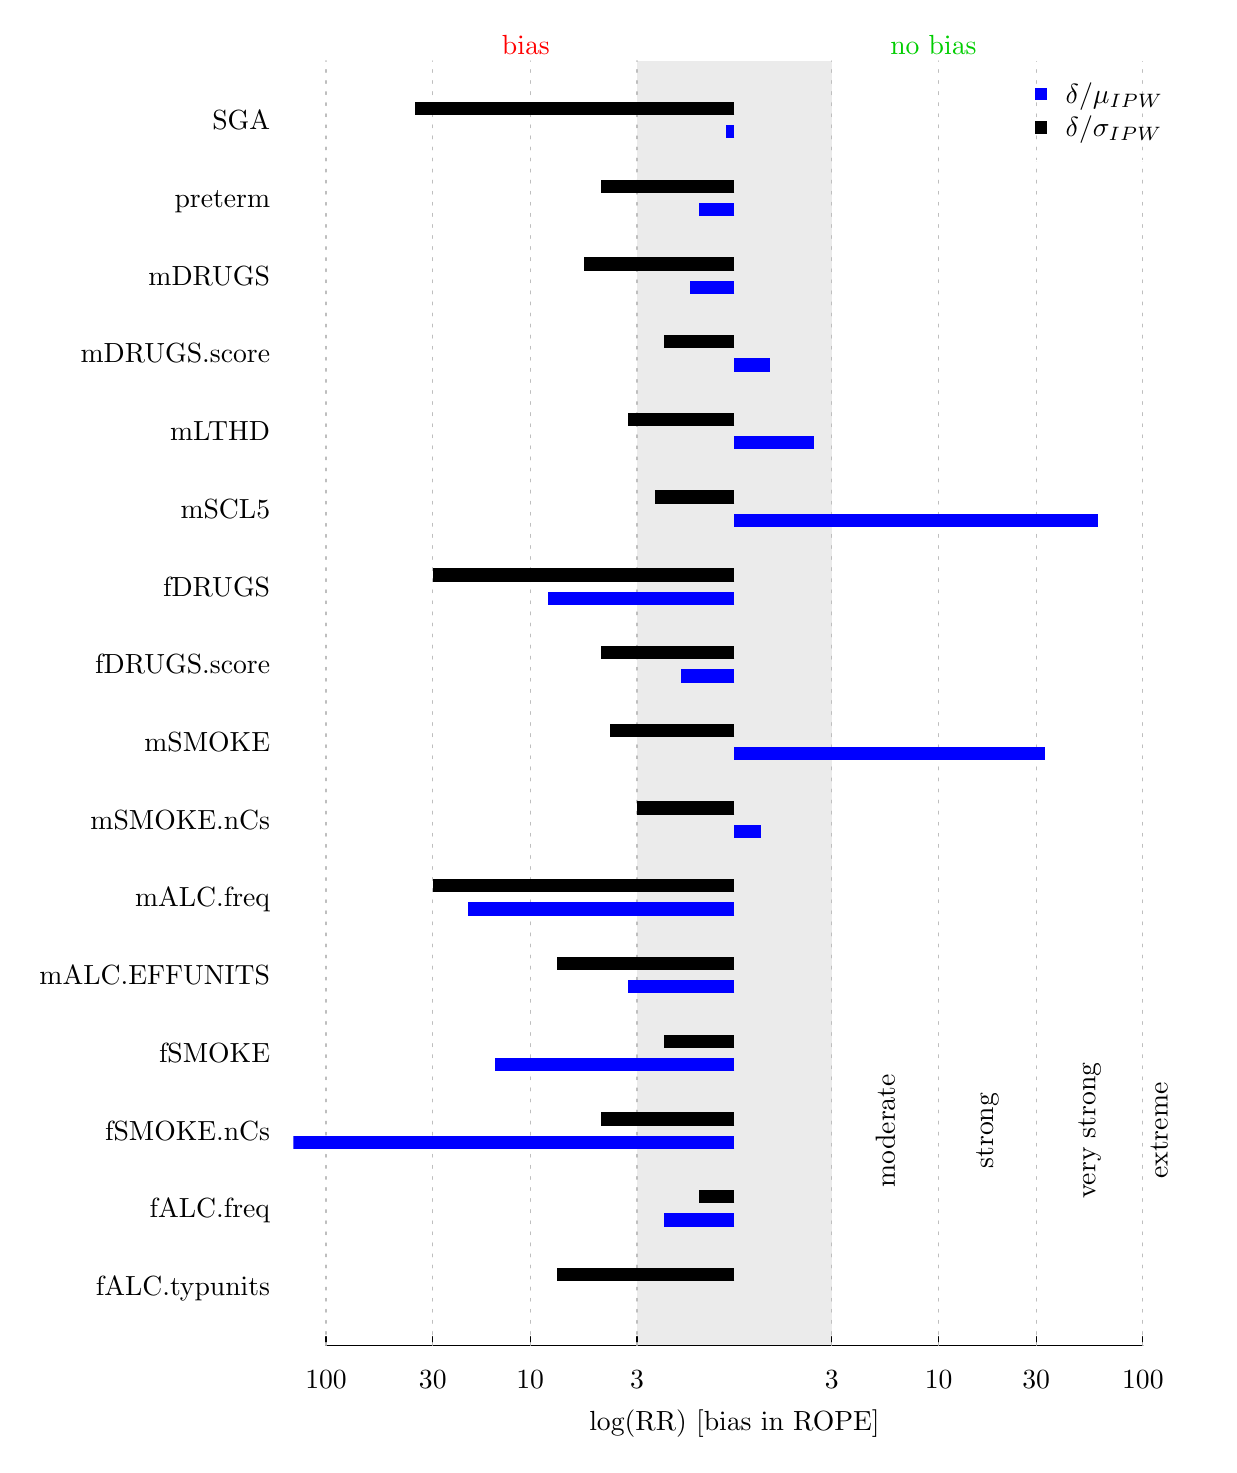
\begin{tikzpicture}[x=1pt,y=1pt]
\definecolor{fillColor}{RGB}{255,255,255}
\path[use as bounding box,fill=fillColor,fill opacity=0.00] (0,0) rectangle (426.79,512.15);
\begin{scope}
\path[clip] (  0.00,  0.00) rectangle (426.79,512.15);
\definecolor{drawColor}{RGB}{0,0,0}

\node[text=drawColor,anchor=base,inner sep=0pt, outer sep=0pt, scale=  1.00] at (255.40,  5.40) {log(RR) [bias in ROPE]};
\end{scope}
\begin{scope}
\path[clip] ( 96.00, 36.00) rectangle (414.79,500.15);
\definecolor{fillColor}{RGB}{190,190,190}

\path[fill=fillColor,fill opacity=0.30] (220.19, 36.00) rectangle (290.60,500.15);
\end{scope}
\begin{scope}
\path[clip] (  0.00,  0.00) rectangle (426.79,512.15);
\definecolor{drawColor}{RGB}{0,0,0}

\path[draw=drawColor,line width= 0.4pt,line join=round,line cap=round] (107.81, 36.00) -- (402.98, 36.00);

\path[draw=drawColor,line width= 0.4pt,line join=round,line cap=round] (107.81, 36.00) -- (107.81, 39.19);

\path[draw=drawColor,line width= 0.4pt,line join=round,line cap=round] (146.39, 36.00) -- (146.39, 39.19);

\path[draw=drawColor,line width= 0.4pt,line join=round,line cap=round] (181.60, 36.00) -- (181.60, 39.19);

\path[draw=drawColor,line width= 0.4pt,line join=round,line cap=round] (220.19, 36.00) -- (220.19, 39.19);

\path[draw=drawColor,line width= 0.4pt,line join=round,line cap=round] (290.60, 36.00) -- (290.60, 39.19);

\path[draw=drawColor,line width= 0.4pt,line join=round,line cap=round] (329.19, 36.00) -- (329.19, 39.19);

\path[draw=drawColor,line width= 0.4pt,line join=round,line cap=round] (364.40, 36.00) -- (364.40, 39.19);

\path[draw=drawColor,line width= 0.4pt,line join=round,line cap=round] (402.98, 36.00) -- (402.98, 39.19);

\node[text=drawColor,anchor=base,inner sep=0pt, outer sep=0pt, scale=  1.00] at (107.81, 20.40) {100};

\node[text=drawColor,anchor=base,inner sep=0pt, outer sep=0pt, scale=  1.00] at (146.39, 20.40) {30};

\node[text=drawColor,anchor=base,inner sep=0pt, outer sep=0pt, scale=  1.00] at (181.60, 20.40) {10};

\node[text=drawColor,anchor=base,inner sep=0pt, outer sep=0pt, scale=  1.00] at (220.19, 20.40) {3};

\node[text=drawColor,anchor=base,inner sep=0pt, outer sep=0pt, scale=  1.00] at (290.60, 20.40) {3};

\node[text=drawColor,anchor=base,inner sep=0pt, outer sep=0pt, scale=  1.00] at (329.19, 20.40) {10};

\node[text=drawColor,anchor=base,inner sep=0pt, outer sep=0pt, scale=  1.00] at (364.40, 20.40) {30};

\node[text=drawColor,anchor=base,inner sep=0pt, outer sep=0pt, scale=  1.00] at (402.98, 20.40) {100};
\end{scope}
\begin{scope}
\path[clip] ( 96.00, 36.00) rectangle (414.79,500.15);
\definecolor{drawColor}{RGB}{190,190,190}

\path[draw=drawColor,line width= 0.4pt,dash pattern=on 1pt off 3pt ,line join=round,line cap=round] (107.81, 36.00) -- (107.81,500.15);

\path[draw=drawColor,line width= 0.4pt,dash pattern=on 1pt off 3pt ,line join=round,line cap=round] (146.39, 36.00) -- (146.39,500.15);

\path[draw=drawColor,line width= 0.4pt,dash pattern=on 1pt off 3pt ,line join=round,line cap=round] (181.60, 36.00) -- (181.60,500.15);

\path[draw=drawColor,line width= 0.4pt,dash pattern=on 1pt off 3pt ,line join=round,line cap=round] (220.19, 36.00) -- (220.19,500.15);

\path[draw=drawColor,line width= 0.4pt,dash pattern=on 1pt off 3pt ,line join=round,line cap=round] (290.60, 36.00) -- (290.60,500.15);

\path[draw=drawColor,line width= 0.4pt,dash pattern=on 1pt off 3pt ,line join=round,line cap=round] (329.19, 36.00) -- (329.19,500.15);

\path[draw=drawColor,line width= 0.4pt,dash pattern=on 1pt off 3pt ,line join=round,line cap=round] (364.40, 36.00) -- (364.40,500.15);

\path[draw=drawColor,line width= 0.4pt,dash pattern=on 1pt off 3pt ,line join=round,line cap=round] (402.98, 36.00) -- (402.98,500.15);
\end{scope}
\begin{scope}
\path[clip] (  0.00,  0.00) rectangle (426.79,512.15);
\definecolor{drawColor}{RGB}{255,0,0}

\node[text=drawColor,anchor=base,inner sep=0pt, outer sep=0pt, scale=  1.00] at (180.02,502.55) {bias};
\definecolor{drawColor}{RGB}{0,205,0}

\node[text=drawColor,anchor=base east,inner sep=0pt, outer sep=0pt, scale=  1.00] at (342.88,502.55) {no bias};
\definecolor{drawColor}{RGB}{0,0,0}

\node[text=drawColor,anchor=base east,inner sep=0pt, outer sep=0pt, scale=  1.00] at ( 87.60, 53.96) {fALC.typunits};

\node[text=drawColor,anchor=base east,inner sep=0pt, outer sep=0pt, scale=  1.00] at ( 87.60, 82.05) {fALC.freq};

\node[text=drawColor,anchor=base east,inner sep=0pt, outer sep=0pt, scale=  1.00] at ( 87.60,110.14) {fSMOKE.nCs};

\node[text=drawColor,anchor=base east,inner sep=0pt, outer sep=0pt, scale=  1.00] at ( 87.60,138.23) {fSMOKE};

\node[text=drawColor,anchor=base east,inner sep=0pt, outer sep=0pt, scale=  1.00] at ( 87.60,166.32) {mALC.EFFUNITS};

\node[text=drawColor,anchor=base east,inner sep=0pt, outer sep=0pt, scale=  1.00] at ( 87.60,194.41) {mALC.freq};

\node[text=drawColor,anchor=base east,inner sep=0pt, outer sep=0pt, scale=  1.00] at ( 87.60,222.50) {mSMOKE.nCs};

\node[text=drawColor,anchor=base east,inner sep=0pt, outer sep=0pt, scale=  1.00] at ( 87.60,250.59) {mSMOKE};

\node[text=drawColor,anchor=base east,inner sep=0pt, outer sep=0pt, scale=  1.00] at ( 87.60,278.68) {fDRUGS.score};

\node[text=drawColor,anchor=base east,inner sep=0pt, outer sep=0pt, scale=  1.00] at ( 87.60,306.77) {fDRUGS};

\node[text=drawColor,anchor=base east,inner sep=0pt, outer sep=0pt, scale=  1.00] at ( 87.60,334.85) {mSCL5};

\node[text=drawColor,anchor=base east,inner sep=0pt, outer sep=0pt, scale=  1.00] at ( 87.60,362.94) {mLTHD};

\node[text=drawColor,anchor=base east,inner sep=0pt, outer sep=0pt, scale=  1.00] at ( 87.60,391.03) {mDRUGS.score};

\node[text=drawColor,anchor=base east,inner sep=0pt, outer sep=0pt, scale=  1.00] at ( 87.60,419.12) {mDRUGS};

\node[text=drawColor,anchor=base east,inner sep=0pt, outer sep=0pt, scale=  1.00] at ( 87.60,447.21) {preterm};

\node[text=drawColor,anchor=base east,inner sep=0pt, outer sep=0pt, scale=  1.00] at ( 87.60,475.30) {SGA};
\end{scope}
\begin{scope}
\path[clip] ( 96.00, 36.00) rectangle (414.79,500.15);
\definecolor{drawColor}{RGB}{0,0,255}

\path[draw=drawColor,line width= 4.8pt,line join=round] (255.40,474.53) -- (252.19,474.53);

\path[draw=drawColor,line width= 4.8pt,line join=round] (255.40,446.44) -- (242.58,446.44);

\path[draw=drawColor,line width= 4.8pt,line join=round] (255.40,418.35) -- (239.37,418.35);

\path[draw=drawColor,line width= 4.8pt,line join=round] (255.40,390.26) -- (268.22,390.26);

\path[draw=drawColor,line width= 4.8pt,line join=round] (255.40,362.17) -- (284.24,362.17);

\path[draw=drawColor,line width= 4.8pt,line join=round] (255.40,334.08) -- (386.79,334.08);

\path[draw=drawColor,line width= 4.8pt,line join=round] (255.40,306.00) -- (188.09,306.00);

\path[draw=drawColor,line width= 4.8pt,line join=round] (255.40,277.91) -- (236.17,277.91);

\path[draw=drawColor,line width= 4.8pt,line join=round] (255.40,249.82) -- (367.57,249.82);

\path[draw=drawColor,line width= 4.8pt,line join=round] (255.40,221.73) -- (265.01,221.73);

\path[draw=drawColor,line width= 4.8pt,line join=round] (255.40,193.64) -- (159.25,193.64);

\path[draw=drawColor,line width= 4.8pt,line join=round] (255.40,165.55) -- (216.94,165.55);

\path[draw=drawColor,line width= 4.8pt,line join=round] (255.40,137.46) -- (168.86,137.46);

\path[draw=drawColor,line width= 4.8pt,line join=round] (255.40,109.37) -- ( 72.72,109.37);

\path[draw=drawColor,line width= 4.8pt,line join=round] (255.40, 81.28) -- (229.76, 81.28);

\path[draw=drawColor,line width= 4.8pt,line join=round] (255.40, 53.19) -- (255.40, 53.19);
\definecolor{drawColor}{RGB}{0,0,0}

\path[draw=drawColor,line width= 4.8pt,line join=round] (255.40,482.96) -- (140.02,482.96);

\path[draw=drawColor,line width= 4.8pt,line join=round] (255.40,454.87) -- (207.32,454.87);

\path[draw=drawColor,line width= 4.8pt,line join=round] (255.40,426.78) -- (200.91,426.78);

\path[draw=drawColor,line width= 4.8pt,line join=round] (255.40,398.69) -- (229.76,398.69);

\path[draw=drawColor,line width= 4.8pt,line join=round] (255.40,370.60) -- (216.94,370.60);

\path[draw=drawColor,line width= 4.8pt,line join=round] (255.40,342.51) -- (226.55,342.51);

\path[draw=drawColor,line width= 4.8pt,line join=round] (255.40,314.42) -- (146.43,314.42);

\path[draw=drawColor,line width= 4.8pt,line join=round] (255.40,286.33) -- (207.32,286.33);

\path[draw=drawColor,line width= 4.8pt,line join=round] (255.40,258.24) -- (210.53,258.24);

\path[draw=drawColor,line width= 4.8pt,line join=round] (255.40,230.15) -- (220.14,230.15);

\path[draw=drawColor,line width= 4.8pt,line join=round] (255.40,202.06) -- (146.43,202.06);

\path[draw=drawColor,line width= 4.8pt,line join=round] (255.40,173.98) -- (191.30,173.98);

\path[draw=drawColor,line width= 4.8pt,line join=round] (255.40,145.89) -- (229.76,145.89);

\path[draw=drawColor,line width= 4.8pt,line join=round] (255.40,117.80) -- (207.32,117.80);

\path[draw=drawColor,line width= 4.8pt,line join=round] (255.40, 89.71) -- (242.58, 89.71);

\path[draw=drawColor,line width= 4.8pt,line join=round] (255.40, 61.62) -- (191.30, 61.62);
\end{scope}
\begin{scope}
\path[clip] (  0.00,  0.00) rectangle (426.79,512.15);
\definecolor{drawColor}{RGB}{0,0,0}

\node[text=drawColor,rotate= 90.00,anchor=base,inner sep=0pt, outer sep=0pt, scale=  1.00] at (313.34,113.58) {moderate};

\node[text=drawColor,rotate= 90.00,anchor=base,inner sep=0pt, outer sep=0pt, scale=  1.00] at (348.90,113.58) {strong};

\node[text=drawColor,rotate= 90.00,anchor=base,inner sep=0pt, outer sep=0pt, scale=  1.00] at (385.79,113.58) {very strong};

\node[text=drawColor,rotate= 90.00,anchor=base,inner sep=0pt, outer sep=0pt, scale=  1.00] at (411.96,113.58) {extreme};
\definecolor{drawColor}{RGB}{255,255,255}

\path[draw=drawColor,line width= 0.4pt,line join=round,line cap=round] (357.09,500.15) rectangle (414.79,464.15);
\definecolor{fillColor}{RGB}{0,0,255}

\path[fill=fillColor] (363.84,485.90) --
	(368.34,485.90) --
	(368.34,490.40) --
	(363.84,490.40) --
	cycle;
\definecolor{fillColor}{RGB}{0,0,0}

\path[fill=fillColor] (363.84,473.90) --
	(368.34,473.90) --
	(368.34,478.40) --
	(363.84,478.40) --
	cycle;
\definecolor{drawColor}{RGB}{0,0,0}

\node[text=drawColor,anchor=base west,inner sep=0pt, outer sep=0pt, scale=  1.00] at (375.09,484.71) {$\delta/\mu_{IPW}$};

\node[text=drawColor,anchor=base west,inner sep=0pt, outer sep=0pt, scale=  1.00] at (375.09,472.71) {$\delta/\sigma_{IPW}$};
\end{scope}
\end{tikzpicture}

	}
	\caption{Evidence for and against selection bias. To obtain a measure of evidence for or against selection bias, we compare how much of the posterior distribution of the difference between the IPW and AR estimates fall within vs fall outside the region of practical equivalence: $log(RR) = logit(\int_{-.5}^{.5}\delta)$. Categorization into positive, strong, or very strong evidence is based on \supercite{Kass1995-uv}. Standard deviation (mean) standardized bias estimates are shown in in blue (black).} 
	\label{fig:logRRs}
\end{figure}



\begin{figure}[ht]
	\centering % Created by tikzDevice version 0.12 on 2019-01-18 11:36:19
% !TEX encoding = UTF-8 Unicode

	\caption{Evidence for and against selection bias for alternative ROPE boundaries. Each plot has the (absolute) ROPE boundary on the x axis and the proportion of the posterior distribution of the bias estimate on the y axis. Blue curves are for mean standardized bias estimates ($\delta/\mu_{IPW}$) and black for standard deviation standardized estimates ($\delta/\sigma_{IPW}$). The red dotted line marks the ROPE boundary of 0.5 used in the presented analysis. Squares (triangles) on the x axis mark ROPE boundaries at which the ROPE would include (exclude) 90\% of the posterior distribution of the bias estimate fall.}
	\label{fig:ropeplots}
\end{figure}


\end{document}
